% course-id: d90.o015.course.id-ID
% canonical-spine: Andreas Habring, arXiv:2607.11664v1, CC BY 4.0
% bounded-supplement: Stephen Becker / Mitchell Krock, MIT License
% independent-completion-layer: CC BY-SA 4.0
\NewTaggingSocket{minipage/before}{0}
\NewTaggingSocket{minipage/after}{0}
\NewTaggingSocket{parbox/before}{0}
\NewTaggingSocket{parbox/after}{0}
\DocumentMetadata{lang=id-ID,tagging=on}
\documentclass[11pt,a4paper,oneside,openany]{book}
% Lapisan pembaca terpadu dan penandaan aksesibilitas O015/D90.
% Toolchain MiKTeX pada mesin produksi tidak sinkron dengan modul latex-lab
% terbaru. Loader kompatibilitas lokal menyediakan struktur tingkat rendah;
% karena itu dokumen ini bertanda dan dapat dicari, tetapi tidak mengklaim
% kesesuaian PDF/UA tanpa validator kesesuaian yang dipatok.
\usepackage[indonesian]{babel}
\usepackage{amsmath,amsthm,mathtools}
\numberwithin{equation}{chapter}
\usepackage[T1]{fontenc}
\usepackage[proportional]{libertine}
\usepackage[libertine,smallerops,liby,vvarbb]{newtxmath}
% The legacy Inconsolata package exposes only T1 families on this LuaLaTeX
% toolchain and therefore falls back for TU texttt.  Use a bundled OpenType
% monospaced face explicitly for a stable searchable code surface.
\setmonofont[Scale=0.95]{Latin Modern Mono}
\usepackage{microtype}
\usepackage[a4paper,top=18mm,bottom=19mm,left=20mm,right=20mm,headheight=15pt]{geometry}
\usepackage{graphicx}
\usepackage[svgnames]{xcolor}
\definecolor{structure}{RGB}{30,55,125}
\definecolor{linkcolor}{RGB}{0,76,147}
\usepackage{csquotes}
\usepackage{algorithm}
\usepackage[labelfont={color=structure,sf}]{caption}
\usepackage[labelfont={color=structure,sf}]{subcaption}
\usepackage{etoolbox}
\usepackage{fancyhdr}
\usepackage[
  colorlinks=true,
  linkcolor=linkcolor,
  citecolor=linkcolor,
  urlcolor=linkcolor,
  filecolor=linkcolor,
  unicode=true,
  pdfencoding=auto,
  linktocpage=true
]{hyperref}
\usepackage[nameinlink,capitalise]{cleveref}
\usepackage[backend=biber,style=authoryear,maxbibnames=99,giveninits=true,isbn=false]{biblatex}
\newcommand{\OIntegratedReader}{}
\usepackage{tikz}
\usepackage{pgfplots}
\usepgfplotslibrary{groupplots}
\pgfplotsset{compat=1.18}
\usetikzlibrary{intersections,calc}
\usetikzlibrary{arrows.meta, decorations.markings}
\usepackage{glossaries-extra}
\usepackage{needspace}

\newcommand{\half}{\frac{1}{2}}
\newcommand{\N}{\mathbb{N}}
\newcommand{\Z}{\mathbb{Z}}
\newcommand{\Q}{\mathbb{Q}}
\newcommand{\R}{\mathbb{R}}
\newcommand{\Rb}{\overline{\mathbb{R}}}
\newcommand{\bR}{\overline{\mathbb{R}}}
\newcommand{\F}{\mathbb{F}}
\newcommand{\1}{\mathbb{1}}
\newcommand{\linop}{\mathcal{L}}
\newcommand{\Rnn}{\mathbb{R}^{n\times n}}
\newcommand{\Cnn}{\mathbb{C}^{n\times n}}
\newcommand{\E}{\mathbb{E}}
\usepackage{pgffor}
\foreach \x in {A,...,Z}{%
    \expandafter\xdef\csname cal\x\endcsname{\noexpand\ensuremath{\noexpand\mathcal{\x}}}
}

\renewcommand{\implies}{\Rightarrow}
\newcommand{\setto}{\rightrightarrows}
\newcommand{\equivalent}{\Leftrightarrow}
\newcommand{\eps}{\varepsilon}
\renewcommand{\phi}{\varphi}
\newcommand{\supp}{\operatorname{\mathrm{supp}}}
\renewcommand{\div}{\operatorname{\mathrm{div}}}
\newcommand{\dom}{\operatorname{\mathrm{dom}}}
\renewcommand{\ker}{\operatorname{\mathrm{ker}}}
\newcommand{\conv}{\operatorname{\mathrm{conv}}}
\newcommand{\rg}{\operatorname{\mathrm{rg}}}
\newcommand{\graph}{\operatorname{\mathrm{graph}}}
\newcommand{\tr}{\operatorname{\mathrm{tr}}}
\newcommand{\epi}{\operatorname{\mathrm{epi}}}
% Never redefine TeX's primitive \span: amsmath alignment environments use it.
% Use \spann for the linear-span operator in reader prose and formulae.
\newcommand{\sign}{\operatorname{\mathrm{sign}}}
\DeclareMathOperator{\Id}{\mathrm{Id}}
\newcommand{\prox}{\mathrm{prox}}
\newcommand{\proj}{\mathrm{proj}}
\newcommand{\spann}{\operatorname{\mathrm{span}}}
\newcommand{\Lloc}{L^1_{\mathrm{loc}}}
\newcommand{\Cinf}{C^\infty_0}

% Nama lingkungan dilokalkan; penomoran dan topologi sumber dipertahankan.
\newtheorem{theorem}{Teorema}[chapter]
\newtheorem{lemma}[theorem]{Lema}
\newtheorem{cor}[theorem]{Korolari}
\theoremstyle{definition}
\newtheorem{defn}[theorem]{Definisi}
\newtheorem{prop}[theorem]{Proposisi}
\newtheorem{example}[theorem]{Contoh}
\newtheorem{assumption}[theorem]{Asumsi}
\newtheorem{exercise}[theorem]{Latihan}
\newtheorem*{rem}{Catatan}

\crefname{theorem}{teorema}{teorema}
\Crefname{theorem}{Teorema}{Teorema}
\crefname{lemma}{lema}{lema}
\Crefname{lemma}{Lema}{Lema}
\crefname{cor}{korolari}{korolari}
\Crefname{cor}{Korolari}{Korolari}
\crefname{prop}{proposisi}{proposisi}
\Crefname{prop}{Proposisi}{Proposisi}
\crefname{defn}{definisi}{definisi}
\Crefname{defn}{Definisi}{Definisi}
\crefname{example}{contoh}{contoh}
\Crefname{example}{Contoh}{Contoh}
\crefname{assumption}{asumsi}{asumsi}
\Crefname{assumption}{Asumsi}{Asumsi}
\crefname{rem}{catatan}{catatan}
\Crefname{rem}{Catatan}{Catatan}
\crefname{exercise}{latihan}{latihan}
\Crefname{exercise}{Latihan}{Latihan}

\renewcommand{\proofname}{Bukti}
\renewcommand{\contentsname}{Daftar Isi}
\renewcommand{\figurename}{Gambar}

\newcommand{\norm}[1]{\|#1\|}
\newcommand{\abs}[1]{\left|#1\right|}
\newcommand{\inner}[2]{\left\langle#1 , #2\right\rangle}
\newcommand{\dual}[1]{\langle #1 \rangle}
\newcommand{\setof}[2]{\left\{#1 \;\middle|\; #2\right\}}
\newcommand{\wkto}{\rightharpoonup}
\DeclareMathOperator{\Exp}{\mathbb{E}}
\DeclareMathOperator{\Var}{\mathbb{V}}
\DeclareMathOperator{\Cov}{\mathrm{Cov}}
\newcommand{\Prob}{\mathbb{P}}

\usepackage{enumerate}
\newcommand{\weaki}{\protect{\u{\i}}}
\AtBeginEnvironment{remark}{\small}

\ifdefined\OIntegratedReader
  % Keep examples as ordinary theorem blocks in the tagged master. The legacy
  % mdframed/tablefootnote patches interfere with the synchronized latex-lab
  % hooks, while no canonical body calls \tablefootnote.
\else
  \usepackage{mdframed}
  \mdfdefinestyle{examplebg}{
      backgroundcolor=structure!7,%
      hidealllines=true,%
      splittopskip=\topskip,
      frametitleaboveskip=0,
      frametitlebelowskip=0,
      innertopmargin=-.3em,%
      innerbottommargin=.7em,%
      innerleftmargin=.7em,%
      innerrightmargin=.7em,%
  }
  \surroundwithmdframed[style=examplebg]{example}
  \usepackage{tablefootnote}
  \makeatletter
  \AfterEndEnvironment{mdframed}{%
   \tfn@tablefootnoteprintout%
   \gdef\tfn@fnt{0}%
  }
  \makeatother
\fi

\usepackage{enumitem}
\setlist[enumerate]{label=(\roman*)}
\usepackage{scrhack}

\newcommand{\ie}{\textit{yaitu}}
\newcommand{\eg}{\textit{misalnya}}
\newcommand{\cf}{\textit{bandingkan}}
\newcommand{\emptyarg}{\,\cdot\,}
\newcommand{\dd}{\mathrm{d}}
\newcommand{\todo}[1]{{\color{red}Perlu dikerjakan: #1}}
\newcommand{\Oc}{\mathcal{O}}
\newcommand{\Lc}{\mathcal{L}}
\newcommand{\Gc}{\mathcal{G}}
\newcommand{\Ic}{\mathcal{I}}
\newcommand{\Pc}{\mathcal{P}}
\newcommand{\Mc}{\mathcal{M}}
\renewcommand{\epsilon}{\varepsilon}
\newcommand{\diag}{\mathrm{diag}}


\microtypesetup{expansion=false}
\frenchspacing
\raggedbottom
\setlength{\emergencystretch}{3em}
\setcounter{tocdepth}{1}
\setcounter{secnumdepth}{3}
\glsdisablehyper

\pagestyle{fancy}
\fancyhf{}
\fancyhead[L]{\small\sffamily\color{structure}\nouppercase{\leftmark}}
\fancyhead[R]{\small\sffamily\color{structure}\thepage}
\renewcommand{\headrulewidth}{0.4pt}
\renewcommand{\chaptermark}[1]{\markboth{\thechapter\enspace #1}{}}
\renewcommand{\chaptername}{Bab}
\renewcommand{\contentsname}{Daftar Isi}
\renewcommand{\figurename}{Gambar}
\renewcommand{\proofname}{Bukti}

% Restore the standard book footnote template after package hooks so the
% synchronized latex-lab compatibility layer can recognize and tag it.
\makeatletter
\renewcommand\@makefntext[1]{%
  \parindent 1em\noindent
  \hb@xt@1.8em{\hss\@makefnmark}#1}
\makeatother

\ifdefined\ONoManualMC
  \newcommand{\OBeginStructure}[1]{%
    \tagstructbegin{tag=Part,title={#1}}%
    \tagstructbegin{tag=Sect,title={#1}}%
  }
  \newcommand{\OEndStructure}{%
    \tagstructend%
    \tagstructend%
  }
\else
  \newcommand{\OBeginStructure}[1]{%
    \tagstructbegin{tag=Part,title={#1}}%
    \tagstructbegin{tag=Sect,title={#1}}%
    \tagstructbegin{tag=P}%
    \tagmcbegin{tag=P}%
  }
  \newcommand{\OEndStructure}{%
    \tagmcend%
    \tagstructend%
    \tagstructend%
    \tagstructend%
  }
\fi

\addbibresource{references-integrated-id.bib}

\title{Optimisasi Lanjut dan Analisis Konveks}
\author{Andreas Habring; Stephen Becker; Mitchell Krock\\
  dengan lapisan penghubung dan asesmen mandiri}
\date{Edisi Bahasa Indonesia (id-ID), 26 Agustus 2026}
\hypersetup{
  pdflang={id-ID},
  pdftitle={Optimisasi Lanjut dan Analisis Konveks - Edisi Bahasa Indonesia},
  pdfauthor={Andreas Habring; Stephen Becker; Mitchell Krock},
  pdfsubject={Buku kursus optimisasi lanjut dan analisis konveks},
  pdfkeywords={optimisasi konveks, metode proksimal, dualitas, metode stokastik, operator monoton, transportasi optimal},
  pdfcreator={OpenAI Codex gpt-5.6-sol, Ultra}
}

\begin{document}
\tagpdfsetup{para/tagging=false}

\OBeginStructure{Bagian awal}
\hypersetup{pageanchor=false}
\frontmatter
\maketitle
\hypersetup{pageanchor=true}
\chapter*{Tentang edisi ini}
\addcontentsline{toc}{chapter}{Tentang edisi ini}
Buku ini adalah edisi Bahasa Indonesia mandiri untuk belajar optimisasi lanjut
dan analisis konveks. Tulang punggung terstruktur menerjemahkan lengkap catatan
Andreas Habring, arXiv:2607.11664v1, berdasarkan CC BY 4.0. Tiga suplemen
terbatas dari catatan Stephen Becker yang diketik Mitchell Krock digunakan
berdasarkan Lisensi MIT. Bab penghubung, asesmen, solusi, laboratorium, dan
proyek yang ditulis khusus untuk edisi ini tersedia berdasarkan CC BY-SA 4.0.
Hak setiap komponen tetap terpisah; tidak ada klaim lisensi payung.

Edisi ini bukan karya resmi atau dukungan Habring, Becker, Krock, institusi
mereka, maupun penyedia sumber pendamping. Materi MIT OpenCourseWare, Clément
Royer, dan Penn State dipertahankan sebagai pembaca pendamping terpisah dan
tidak disisipkan diam-diam ke dalam buku kanonis ini. Materi O018 tentang
program linear atau bilangan bulat, simpleks, sensitivitas LP, dan optimisasi
jaringan berada di luar cakupan.

Produksi edisi dan pemeriksaan deterministik menggunakan OpenAI Codex
gpt-5.6-sol, Ultra. Kredit pengarang sumber dan kontribusi manusia tetap
dipertahankan. Perubahan substantif dan koreksi didokumentasikan dalam berkas
provenans edisi.

PDF ini menyediakan teks yang dapat dicari, bahasa dokumen id-ID, markah,
bookmark, tautan, dan pohon struktur berurutan. Karena validator PDF/UA yang
dipatok tidak tersedia pada toolchain produksi, edisi ini tidak mengklaim
kesesuaian PDF/UA. HTML dan EPUB 3 menyediakan permukaan reflow utama.

\chapter*{Deskripsi gambar raster}
\addcontentsline{toc}{chapter}{Deskripsi gambar raster}
Enam gambar raster dari tulang punggung mempunyai keterangan dan uraian
sekitar. Secara ringkas: \emph{sets.png} membandingkan contoh himpunan konveks
dan tak konveks; \emph{balls.png} membandingkan bola satuan beberapa norma;
\emph{convex\_fct.png} menunjukkan grafik fungsi konveks dan garis tali
busurnya; \emph{gradient.png} menunjukkan gradien sebagai penyangga lokal;
\emph{subgradient.png} menunjukkan keluarga subgradien pada titik tak mulus;
\emph{discontinuous\_function.png} dan \emph{lsc\_function.png} membandingkan
fungsi diskontinu dengan fungsi semikontinu bawah. Gambar TikZ dan grafik
komputasi dijelaskan oleh keterangan serta teks yang langsung mendahului atau
mengikutinya.

\tableofcontents
\OEndStructure

\mainmatter
\OBeginStructure{Tulang punggung Habring}
\part{Tulang Punggung: Optimisasi Konveks}
% H01-S001 | sumber authority/habring/source-v1/preface.tex baris 1--8
% segment-id: d90.hab.v1.ch01.seg0001
\chapter*{Prakata}
\markboth{Prakata}{Prakata}
\enlargethispage*{2cm}

Catatan ini dibangun di atas slide kuliah yang disusun oleh Prof.~Thomas Pock.
Naskah ini belum merupakan versi final dan mungkin masih memuat salah ketik atau
kesalahan, serta kekurangan \emph{teks penghubung} di antara hasil-hasilnya. Catatan
ini terutama berfungsi sebagai kumpulan materi untuk kuliah terkait yang saya ampu
pada semester musim panas 2026 di Graz University of Technology.

Saya berterima kasih kepada Prof.~Christian Clason atas templat \LaTeX{} yang indah ini.

% H01-S002 | sumber authority/habring/source-v1/preliminaries.tex baris 1--197
% segment-id: d90.hab.v1.ch01.seg0002
\chapter{Prasyarat}

\section{Ruang vektor, norma, dan hasil kali dalam}

\begin{defn}[Ruang vektor]\label{preliminaries:defn:vectorspace}
    Ruang vektor atas suatu medan $\mathbb{F}$ adalah himpunan $V$ yang dilengkapi
    dengan dua operasi
    $+:V\times V\rightarrow V$, $(u,v)\mapsto u+v$, dan
    $\cdot:\mathbb{F}\times V\rightarrow V$,
    $(\lambda,v)\mapsto\lambda\cdot v$, sedemikian sehingga
    \begin{enumerate}
        \item $(V,+)$ merupakan grup Abel; yaitu, untuk setiap $u,v,w\in V$ berlaku:
        \begin{enumerate}
            \item Asosiativitas: $(u+v)+w=u+(v+w)$.
            \item Unsur netral: terdapat $e\in V$ sehingga
            $v+e=e+v=v$. Kita menuliskan $e=0$.
            \item Unsur invers: terdapat $\widetilde v\in V$ sehingga
            $v+\widetilde v=0$. Kita menuliskan $\widetilde v=-v$.
            \item Komutativitas: $v+w=w+v$.
        \end{enumerate}
        \item Hukum-hukum skalar berikut berlaku untuk setiap $u,v\in V$ dan
        $\lambda,\mu\in\mathbb{F}$:
        \begin{enumerate}
            \item $\lambda\cdot(\mu\cdot v)=(\lambda\mu)\cdot v$.
            \item $\lambda\cdot(u+v)=(\lambda\cdot u)+(\lambda\cdot v)$.
            \item $(\lambda+\mu)\cdot v=(\lambda\cdot v)+(\mu\cdot v)$.
            \item $1\cdot v=v$.
        \end{enumerate}
    \end{enumerate}
    Kita menuliskan $\lambda\cdot v=\lambda v$.
\end{defn}

Mulai sekarang kita membatasi pembahasan pada $\F=\R$.

\begin{example}[Ruang-ruang vektor penting]
    \begin{enumerate}
        \item $\R^d$: ruang vektor yang terdiri atas vektor berbentuk
        \begin{equation}
            v=\begin{pmatrix}
                v_1\\
                \vdots\\
                v_d
            \end{pmatrix},
        \end{equation}
        dengan $v_i\in\R$, penjumlahan dilakukan komponen demi komponen, dan
        perkalian skalar diterapkan pada setiap komponen. Suatu hasil matematika
        penting menyatakan bahwa setiap ruang vektor berdimensi hingga dapat
        diidentifikasi dengan $\R^d$, dengan $d$ dimensinya. Karena itu, ketika
        bekerja dengan ruang berdimensi hingga, kita biasanya dapat membayangkan
        $\R^d$.

        \item Ruang fungsi: misalkan $\Omega\subset\R^d$ dan
        $f,g:\Omega\rightarrow\R$. Kita dapat mendefinisikan $f+g$ serta, untuk
        $\lambda\in\R$, $\lambda f$ secara titik demi titik melalui
        \begin{gather}
            (f+g)(x)=f(x)+g(x),\\
            (\lambda f)(x)=\lambda f(x).
        \end{gather}
        Dengan cara ini kita dapat membentuk berbagai ruang fungsi. Salah satu
        contohnya ialah ruang fungsi linear. Mengapa ini benar-benar merupakan
        ruang vektor yang terdefinisi dengan baik?
    \end{enumerate}
\end{example}

\begin{defn}[Norma]
    Norma adalah fungsi $\|\emptyarg\|:V\rightarrow[0,\infty)$ sedemikian sehingga,
    untuk setiap $\lambda\in\R$ dan $u,v\in V$, berlaku
    \begin{enumerate}
        \item Ketegasan positif: $\|v\|=0$ jika dan hanya jika $v=0$.
        \item Homogenitas: $\|\lambda u\|=|\lambda|\|u\|$.
        \item Ketaksamaan segitiga: $\|u+v\|\leq\|u\|+\|v\|$.
    \end{enumerate}
    Pasangan $(V,\|\emptyarg\|)$ disebut ruang bernorma.
\end{defn}

\begin{rem}
    Berdasarkan kodomainnya, norma selalu tak negatif.
\end{rem}

Mulai sekarang semua ruang vektor dianggap bernorma. Jika tidak menimbulkan
ambiguitas, kita cukup menuliskan normanya sebagai $\|\emptyarg\|$. Untuk
menyatakan norma tertentu kita menggunakan, misalnya,
$\|\emptyarg\|_\bigstar$, dengan $\bigstar$ suatu simbol yang menandai norma
tersebut; \cf~\cref{preliminiaries:example:norms}.

\begin{example}[Norma-norma umum]
    \label{preliminiaries:example:norms}
    \begin{enumerate}
        \item Norma $\ell^p$: untuk $p\in[1,\infty)$ kita menuliskan
        \begin{equation}
            \|v\|_p=\bigg(\sum_{i=1}^d|v_i|^p\bigg)^{1/p}.
        \end{equation}
        Untuk $p=\infty$ kita menuliskan
        \begin{equation}
            \|v\|_\infty=\max_{i=1,\dots,d}|v_i|.
        \end{equation}

        \item Tinjau ruang matriks $n\times m$, yaitu $\R^{n\times m}$. Setiap
        matriks $A\in\R^{n\times m}$ dapat diidentifikasi dengan fungsi linear
        melalui
        \begin{equation}
            (Av)_i=\sum_{j=1}^m A_{i,j}v_j,\qquad i=1,\dots,n.
        \end{equation}
        Norma-norma berikut sering digunakan pada $\R^{n\times m}$:
        \begin{itemize}
            \item Norma Frobenius:
            $\|A\|_F=\sqrt{\sum_{i,j}|A_{i,j}|^2}$.
            \item Norma terinduksi: untuk setiap pasangan norma
            $\|\emptyarg\|_a$ pada $\R^m$ dan $\|\emptyarg\|_b$ pada $\R^n$,
            kita mendefinisikan
            \begin{equation}
                \|A\|_{a,b}
                \coloneq\sup_{\|v\|_a\leq1}\|Av\|_b
                =\sup_{v\neq0}\frac{\|Av\|_b}{\|v\|_a}.
            \end{equation}
            Norma terinduksi memenuhi
            $\|Av\|_b\leq\|A\|_{a,b}\|v\|_a$. Jika $a=b$, kita menuliskan
            $\|\emptyarg\|_{a,a}=\|\emptyarg\|_a$. Secara khusus,
            \begin{gather}
                \|A\|_1=\max_j\sum_i|A_{i,j}|,\\
                \|A\|_\infty=\max_i\sum_j|A_{i,j}|,\\
                \|A\|_2=\sqrt{\lambda_{\mathrm{max}}(A^\top A)}.
            \end{gather}
        \end{itemize}
        Di sini $\lambda_{\mathrm{max}}$ menyatakan nilai eigen terbesar.

        \item Untuk fungsi terukur Lebesgue $f:\Omega\rightarrow\R$, dengan
        $\Omega\subset\R^d$ terukur, kita
        dapat mendefinisikan norma $L^p$ melalui
        \begin{equation}
            \|f\|_p=\bigg(\int_\Omega|f(x)|^p\dd x\bigg)^{1/p},
            \qquad 1\leq p<\infty,
        \end{equation}
        dan\footnote{Secara tepat, fungsi-fungsi diidentifikasi apabila sama
        hampir di mana-mana. Norma $L^\infty$ adalah supremum esensial,
        $\|f\|_\infty=\inf_{\substack{N\subset\Omega\\|N|=0}}
        \sup_{x\in\Omega\setminus N}|f(x)|$. Rincian teori ukuran ini tidak
        diperlukan dalam kuliah ini.}
        \begin{equation}
            \|f\|_\infty=\operatorname*{ess\,sup}_{x\in\Omega}|f(x)|.
        \end{equation}
        Dengan mengidentifikasi fungsi-fungsi yang sama hampir di mana-mana,
        $\|\emptyarg\|_p$ mendefinisikan norma pada ruang vektor
        \begin{equation}
            L^p(\Omega)=
            \{f:\Omega\rightarrow\R\mid f\text{ terukur dan }\|f\|_p<\infty\}
            /\!\sim_{\mathrm{a.e.}}.
        \end{equation}
    \end{enumerate}
\end{example}

\begin{theorem}[Ekuivalensi norma]
    Semua norma pada $\R^d$ ekuivalen. Artinya, untuk setiap dua norma
    $\|\emptyarg\|_a$ dan $\|\emptyarg\|_b$, terdapat $m,M>0$ sedemikian
    sehingga untuk setiap $v\in\R^d$ berlaku
    \begin{equation}
        m\|v\|_a\leq\|v\|_b\leq M\|v\|_a.
    \end{equation}
\end{theorem}

\begin{defn}[Hasil kali dalam]
    Pemetaan $\langle\emptyarg,\emptyarg\rangle:V\times V\rightarrow\R$
    disebut hasil kali skalar atau hasil kali dalam jika, untuk setiap
    $u,v,w\in V$ dan skalar yang relevan, berlaku
    \begin{enumerate}
        \item Bilinearitas: pemetaan $w\mapsto\langle w,u\rangle$ dan
        $w\mapsto\langle u,w\rangle$ bersifat linear.
        \item Ketegasan positif: $\langle u,u\rangle\geq0$, dan kesamaan berlaku
        jika dan hanya jika $u=0$.
        \item Simetri: $\langle u,v\rangle=\langle v,u\rangle$.
    \end{enumerate}
    Setiap hasil kali dalam mendefinisikan norma melalui
    $\|v\|\coloneq\sqrt{\inner{v}{v}}$. Dalam hal ini, $V$ disebut ruang hasil
    kali dalam.
\end{defn}

\begin{cor}[Cauchy--Schwarz]
    Pada setiap ruang hasil kali dalam $V$ berlaku
    \begin{equation}
        \inner{v}{w}\leq|\inner{v}{w}|\leq\|v\|\|w\|,
        \qquad v,w\in V,
    \end{equation}
    dan ketaksamaan kedua bersifat ketat apabila $v$ dan $w$ tidak kolinear.
\end{cor}

\begin{proof}
    Kita boleh mengandaikan $v,w\neq0$, sebab jika tidak hasilnya langsung
    berlaku. Untuk setiap $\lambda\in\R$,
    \begin{equation}\label{preliminaries:eq:CS}
        0\leq\inner{v-\lambda w}{v-\lambda w}
        =\|v\|^2-2\lambda\inner{v}{w}+\lambda^2\|w\|^2.
    \end{equation}
    Ambil $\lambda=\inner{v}{w}/\|w\|^2$. Maka
    \begin{equation}
        0\leq\|v\|^2-\frac{|\inner{v}{w}|^2}{\|w\|^2},
    \end{equation}
    yang memberikan $|\inner{v}{w}|\leq\|v\|\|w\|$. Jika $v$ dan $w$
    tidak kolinear, maka $v-\lambda w\neq0$ untuk setiap $\lambda$, sehingga
    ketaksamaan dalam~\eqref{preliminaries:eq:CS}, dan dengan demikian
    ketaksamaan Cauchy--Schwarz, bersifat ketat.
\end{proof}


\begin{theorem}[Hölder]
    Misalkan $p,q\in[1,\infty]$ memenuhi
    $\frac1p+\frac1q=1$\footnote{$p$ dan $q$ disebut \emph{eksponen konjugat
    Hölder}.}. Untuk setiap $u,v\in\R^d$ yang dilengkapi dengan hasil kali dalam
    baku, berlaku
    \begin{equation}
        \inner{u}{v}\leq|\inner{u}{v}|\leq\|u\|_p\|v\|_q.
    \end{equation}
\end{theorem}

\begin{proof}
    Kita membedakan kasus-kasus berikut.
    \begin{itemize}
        \item $p=1$ dan $q=\infty$: dengan mudah diperoleh
        \begin{equation}
            |\inner{u}{v}|
            \leq\sum_i|u_i||v_i|
            \leq\sum_i|u_i|\|v\|_\infty
            =\|v\|_\infty\|u\|_1.
        \end{equation}
        Kasus $p=\infty$, $q=1$ mengikuti dengan menukar $u$ dan $v$.

        \item $1<p<\infty$: ketaksamaan jelas benar jika $u=0$ atau $v=0$,
        sehingga andaikan $u,v\neq0$. Ketaksamaan Young menyatakan bahwa untuk
        eksponen konjugat $1<p,q<\infty$ dan $a,b\geq0$ berlaku
        $ab\leq a^p/p+b^q/q$. Karena itu,
        \begin{equation}\label{eq:prelim:hoelder}
            |\inner{u}{v}|
            \leq\sum_i|u_i||v_i|
            \leq\sum_i\left(\frac{|u_i|^p}{p}+\frac{|v_i|^q}{q}\right)
            =\frac{\|u\|_p^p}{p}+\frac{\|v\|_q^q}{q}.
        \end{equation}
        Mengganti $u$ dengan $u/\|u\|_p$ dan $v$ dengan $v/\|v\|_q$
        dalam~\eqref{eq:prelim:hoelder} memberikan
        \begin{equation}
            \begin{aligned}
                \frac{|\inner{u}{v}|}{\|u\|_p\|v\|_q}
                &=\left|\inner{\frac{u}{\|u\|_p}}
                                  {\frac{v}{\|v\|_q}}\right|\\
                &\leq
                \frac{\left\|u/\|u\|_p\right\|_p^p}{p}
                +\frac{\left\|v/\|v\|_q\right\|_q^q}{q}
                =\frac1p+\frac1q=1.
            \end{aligned}
        \end{equation}
    \end{itemize}
\end{proof}

Dengan ketaksamaan Hölder, kita dapat menunjukkan bahwa norma $\ell^p$
memenuhi ketaksamaan segitiga, yaitu bagian tersulit dalam membuktikan bahwa
besaran tersebut benar-benar merupakan norma.

\begin{theorem}
    Untuk setiap $p\in[1,\infty]$ berlaku
    \begin{equation}
        \|x+y\|_p\leq\|x\|_p+\|y\|_p,
        \qquad x,y\in\R^d.
    \end{equation}
\end{theorem}

\begin{proof}
    Kasus $p\in\{1,\infty\}$ ditinggalkan sebagai latihan sederhana. Jadi,
    andaikan $1<p<\infty$. Kita boleh mengandaikan $\|x+y\|_p\neq0$, sebab
    jika tidak hasilnya langsung berlaku. Dengan ketaksamaan Hölder dan
    hubungan $p-1=p/q$, diperoleh
    \begin{equation}
        \begin{aligned}
            \|x+y\|_p^p
            &=\sum_i|x_i+y_i||x_i+y_i|^{p-1}\\
            &\leq\sum_i|x_i||x_i+y_i|^{p-1}
                 +\sum_i|y_i||x_i+y_i|^{p-1}\\
            &\leq(\|x\|_p+\|y\|_p)
            \bigg(\sum_i|x_i+y_i|^{(p-1)q}\bigg)^{1/q}\\
            &=(\|x\|_p+\|y\|_p)\|x+y\|_p^{p/q}.
        \end{aligned}
    \end{equation}
    Membagi kedua ruas dengan $\|x+y\|_p^{p/q}$ menyelesaikan bukti.
\end{proof}

% H01-S003 | sumber authority/habring/source-v1/preliminaries.tex baris 198--277
% segment-id: d90.hab.v1.ch01.seg0003
\section{Barisan dan topologi dasar}

\begin{defn}[Kekonvergenan barisan]
    Barisan $(x_n)_n\subset\R^d$ disebut konvergen jika terdapat $x\in\R^d$
    sedemikian sehingga untuk setiap $\epsilon>0$ terdapat $N\in\N$ dengan
    \begin{equation}
        n\geq N\quad\Longrightarrow\quad\|x-x_n\|\leq\epsilon.
    \end{equation}
\end{defn}

\begin{rem}
    Berdasarkan ekuivalensi norma, kekonvergenan tidak bergantung pada pilihan
    norma.
\end{rem}

\begin{defn}[Barisan Cauchy]
    Barisan $(x_n)_n\subset V$ disebut barisan Cauchy jika dan hanya jika untuk
    setiap $\epsilon>0$ terdapat $N\in\N$ sedemikian sehingga
    $\|x_n-x_m\|<\epsilon$ bagi setiap $n,m\geq N$.
\end{defn}

Sifat Cauchy serupa dengan kekonvergenan. Namun, perhatikan bahwa sifat Cauchy
dapat dirumuskan tanpa gagasan titik limit. Hasil berikut mudah dibuktikan.

\begin{theorem}
    Setiap barisan konvergen merupakan barisan Cauchy.
\end{theorem}

\begin{proof}
    Misalkan $x_n\rightarrow\hat x$. Ketaksamaan segitiga memberikan
    \begin{equation}
        \|x_n-x_m\|\leq\|x_n-\hat x\|+\|x_m-\hat x\|,
    \end{equation}
    dan kedua suku di ruas kanan dapat dibuat sekecil yang diinginkan dengan
    memilih $n,m$ cukup besar.
\end{proof}

\begin{defn}[Ruang Banach dan Hilbert]
    Ruang bernorma $(V,\|\emptyarg\|)$ disebut ruang Banach jika setiap barisan
    Cauchy konvergen. Artinya, jika $(x_n)_n$ merupakan barisan Cauchy, terdapat
    $x\in V$ sehingga $\|x_n-x\|\rightarrow0$ ketika $n\rightarrow\infty$.
    Jika normanya berasal dari suatu hasil kali dalam, ruang Banach tersebut
    disebut ruang Hilbert.
\end{defn}

\begin{example}
    Ruang $(\R^d,\|\emptyarg\|_p)$ merupakan ruang Banach untuk setiap
    $1\leq p\leq\infty$.
\end{example}

\begin{defn}[Topologi dasar]
    Suatu himpunan $A\subset\R^d$ disebut
    \begin{itemize}
        \item terbuka jika untuk setiap $x\in A$ terdapat $\epsilon>0$ sehingga
        $B_\epsilon(x)\subset A$;
        \item tertutup jika $A^c$ terbuka. Ketertutupan ekuivalen dengan sifat
        berikut: jika $(x_n)_n\subset A$ dan $x_n\rightarrow x\in\R^d$, maka
        $x\in A$.
    \end{itemize}
\end{defn}

\begin{defn}[Kekompakan sekuensial]
    Himpunan $A\subset\R^d$ disebut kompak secara sekuensial jika setiap
    barisan di $A$ mempunyai suatu subbarisan yang konvergen ke titik di $A$.
    Dengan kata lain, untuk setiap $(x_n)_n\subset A$ terdapat subbarisan
    $(x_{n(k)})_k$ dan titik $x\in A$ sedemikian sehingga
    $x_{n(k)}\rightarrow x$.
\end{defn}

\begin{theorem}[Bolzano--Weierstrass]\label{thm:bolzano}
    Dalam ruang vektor berdimensi hingga, setiap barisan terbatas mempunyai
    subbarisan konvergen.
\end{theorem}

\begin{proof}
    Pertama andaikan dimensinya satu, sehingga ruangnya adalah $\R$. Misalkan
    $(x_n)_n\subset\R$ terbatas. Secara induktif kita membangun dua barisan
    $(a_n)_n$ dan $(b_n)_n$ dengan
    $a_n\leq b_n$, $[a_n,b_n]\subset[a_{n-1},b_{n-1}]$,
    $b_n-a_n=(b_{n-1}-a_{n-1})/2$, dan, yang terpenting, $[a_n,b_n]$
    memuat tak hingga banyaknya suku $x_k$ untuk setiap $n$.

    Karena barisan terbatas, pilih $a_0,b_0$ sehingga
    $(x_n)_n\subset[a_0,b_0]$. Jelas interval ini memuat tak hingga banyaknya
    suku $x_k$. Andaikan $a_n,b_n$ telah dipilih dan tetapkan
    $m_n=(a_n+b_n)/2$. Karena $[a_n,b_n]$ memuat tak hingga banyaknya suku
    $x_k$, setidaknya salah satu dari $[a_n,m_n]$ dan $[m_n,b_n]$ juga memuat
    tak hingga banyaknya suku. Pilih interval tersebut sebagai
    $[a_{n+1},b_{n+1}]$.

    Sekarang kita membangun subbarisan $(x_{n(k)})_k$ secara induktif. Pilih
    $n(0)$ sehingga $x_{n(0)}\in[a_0,b_0]$. Jika $n(0),\ldots,n(m)$ telah
    dipilih, tetapkan, misalnya,
    $n(m+1)=\min\{j\in\N\mid j>n(m),\ x_j\in[a_{m+1},b_{m+1}]\}$.
    Pilihan ini selalu mungkin karena interval tersebut memuat tak hingga
    banyaknya suku barisan.

    Akhirnya, ambil sembarang $k\leq\ell$. Karena
    $x_{n(k)},x_{n(\ell)}\in[a_k,b_k]$, berlaku
    \begin{equation}
        |x_{n(k)}-x_{n(\ell)}|
        \leq b_k-a_k=2^{-k}(b_0-a_0).
    \end{equation}
    Jadi $(x_{n(k)})_k$ merupakan barisan Cauchy dan karenanya konvergen.

    Untuk dimensi lebih besar, yaitu $\R^d$, mula-mula pilih subbarisan yang
    komponen pertamanya konvergen. Dari subbarisan itu pilih lagi subbarisan
    yang komponen keduanya konvergen, dan lanjutkan demikian. Subbarisan
    diagonal yang diperoleh setelah langkah ke-$d$ mempunyai semua komponen
    yang konvergen; khususnya, subbarisan itu konvergen dalam norma satu.
    Ekuivalensi norma kemudian memberikan kekonvergenan dalam setiap norma.
\end{proof}

Sebagai akibatnya, kita memperoleh hasil berikut.

\begin{cor}
    Di $\R^d$, suatu himpunan kompak jika dan hanya jika tertutup dan terbatas.
\end{cor}

\begin{proof}
    Misalkan $A\subset\R^d$ tertutup dan terbatas, serta
    $(x_n)_n\subset A$. Berdasarkan keterbatasan dan~\cref{thm:bolzano},
    terdapat subbarisan konvergen; berdasarkan ketertutupan, limitnya berada di
    $A$. Jadi $A$ kompak.

    Sebaliknya, andaikan $A$ kompak. Jika $A$ tidak terbatas, untuk setiap
    $n\in\N$ kita dapat memilih $x_n\in A$ dengan $\|x_n\|\geq n$. Barisan ini
    tidak mempunyai subbarisan konvergen, bertentangan dengan kekompakan. Jadi
    $A$ terbatas. Selanjutnya, misalkan $(x_n)_n\subset A$ dan
    $x_n\rightarrow x\in\R^d$. Berdasarkan kekompakan, $(x_n)_n$ mempunyai
    subbarisan $(x_{n(k)})_k$ yang konvergen ke suatu titik di $A$. Setiap
    subbarisan dari barisan konvergen mempunyai limit yang sama, sehingga
    $x=\lim_kx_{n(k)}\in A$. Jadi $A$ tertutup.
\end{proof}

% H01-S004 | sumber authority/habring/source-v1/preliminaries.tex baris 278--297
% segment-id: d90.hab.v1.ch01.seg0004
\section{Fungsi}

\begin{defn}[Kontinuitas]
    Misalkan $f:V\rightarrow E$ suatu pemetaan di antara dua ruang bernorma.
    Fungsi $f$ disebut kontinu di $v\in V$ jika salah satu dari dua syarat
    ekuivalen berikut dipenuhi:
    \begin{itemize}
        \item untuk setiap barisan $v_n\rightarrow v$, berlaku
        $f(v_n)\rightarrow f(v)$;
        \item untuk setiap $\epsilon>0$ terdapat $\delta>0$ sedemikian sehingga
        \begin{equation}
            \|u-v\|\leq\delta
            \quad\Longrightarrow\quad
            \|f(u)-f(v)\|\leq\epsilon.
        \end{equation}
    \end{itemize}
    Jika $f$ kontinu pada setiap $v\in V$, kita cukup mengatakan bahwa $f$
    kontinu.
\end{defn}

\begin{defn}[Kontinuitas Lipschitz]
    Misalkan $f:V\rightarrow E$ suatu pemetaan di antara dua ruang bernorma.
    Fungsi $f$ disebut kontinu Lipschitz jika terdapat $L\geq0$ sedemikian
    sehingga
    \begin{equation}
        \|f(u)-f(v)\|\leq L\|u-v\|,
        \qquad u,v\in V.
    \end{equation}
\end{defn}

% H01-S005 | sumber authority/habring/source-v1/preliminaries.tex baris 298--409
% segment-id: d90.hab.v1.ch01.seg0005
\subsection{Pemetaan linear dan ruang dual}

\begin{defn}[Pemetaan linear]
    Fungsi $f:\R^n\rightarrow\R^m$ disebut linear jika
    \begin{equation}
        f(\lambda x+\mu y)=\lambda f(x)+\mu f(y),
        \qquad x,y\in\R^n,\quad\lambda,\mu\in\R.
    \end{equation}
\end{defn}

Pemetaan linear dapat diidentifikasi dengan matriks.

\begin{theorem}
    Ruang semua fungsi linear $\R^n\rightarrow\R^m$ isomorfik\footnote{Secara
    informal: keduanya mempunyai struktur yang sama.} dengan ruang semua
    matriks $A\in\R^{m\times n}$.
\end{theorem}

\begin{proof}
    Kita mendefinisikan korespondensi satu-ke-satu dengan mengaitkan setiap
    $f:\R^n\rightarrow\R^m$ pada matriks $A_f$ yang diberikan oleh
    \begin{equation}
        (A_f)_{i,j}=f(e_j)_i.
    \end{equation}
    Pembuktian bahwa korespondensi ini bijektif dan linear ditinggalkan sebagai
    latihan.
\end{proof}

\begin{defn}[Ruang dual]
    Misalkan $V$ suatu ruang bernorma. Ruang dual $V^*$ adalah \textbf{ruang
    vektor} semua fungsional linear kontinu dari $V$ ke $\R$, yaitu
    \begin{equation}
        V^*=\{f:V\rightarrow\R\mid f\text{ linear dan kontinu}\}.
    \end{equation}
    Unsur $V^*$ disebut fungsional linear pada $V$. Norma kanonik pada $V^*$
    adalah norma dual
    \begin{equation}
        \|v^*\|_{V^*}
        \coloneq\sup_{\substack{v\in V\\\|v\|_V\leq1}}|v^*(v)|.
    \end{equation}
    Dengan sedikit penyalahgunaan notasi, penerapan suatu unsur dual juga sering
    ditulis memakai notasi hasil kali dalam:
    \begin{equation}
        \inner{v^*}{v}\coloneq v^*(v).
    \end{equation}
\end{defn}

Langsung dari definisi diperoleh
\begin{equation}
    |v^*(v)|\leq\|v^*\|\|v\|.
\end{equation}

Hasil berikut sangat penting: pada ruang Hilbert, ruang dual dapat
diidentifikasi dengan ruang itu sendiri. Hasil ini juga membenarkan penggunaan
notasi hasil kali dalam untuk penerapan unsur dual.

\begin{theorem}[Riesz]
    Misalkan $V$ ruang Hilbert. Untuk setiap $v^*\in V^*$ terdapat tepat satu
    $v\in V$ sedemikian sehingga
    \begin{equation}
        v^*(w)=\langle v,w\rangle,
        \qquad w\in V.
    \end{equation}
    Pemetaan $v^*\mapsto v$ linear dan memenuhi $\|v\|=\|v^*\|$. Secara
    khusus, $V^*\cong V$.
\end{theorem}

\begin{proof}
    Jika $v^*=0$, ambil $v=0$. Jadi, andaikan $v^*\neq0$. Karena
    $\ker(v^*)$ merupakan subruang tertutup, teorema proyeksi ortogonal pada
    ruang Hilbert memberikan
    $V=\ker(v^*)\oplus\ker(v^*)^\perp$. Komponen ortogonal dari sembarang titik
    di luar kernel tidak nol; setelah dinormalkan, kita memperoleh
    $z\in\ker(v^*)^\perp$ dengan $v^*(z)\neq0$ dan $\|z\|=1$.
    Untuk sembarang $w\in V$,
    \begin{equation}
        v^*\bigl(zv^*(w)-wv^*(z)\bigr)=0,
    \end{equation}
    sehingga, berdasarkan ortogonalitas $z$ terhadap $\ker(v^*)$,
    \begin{equation}
        \inner{zv^*(w)-wv^*(z)}{z}=0.
    \end{equation}
    Akibatnya,
    \begin{equation}
        \begin{aligned}
            v^*(w)
            &=v^*(w)\inner{z}{z}
              =\inner{zv^*(w)}{z}\\
            &=\inner{zv^*(w)-wv^*(z)}{z}
              +\inner{wv^*(z)}{z}\\
            &=\inner{w}{v^*(z)z}.
        \end{aligned}
    \end{equation}
    Jadi $v=v^*(z)z$ merupakan unsur yang dicari. Ketunggalan, linearitas
    pemetaan representasi, dan kesamaan normanya ditinggalkan sebagai latihan.
\end{proof}

\begin{example}[Dual]
    Pada $\R^d$, untuk $1\leq p\leq\infty$, norma dual dari
    $\|\emptyarg\|_p$ tepat sama dengan $\|\emptyarg\|_q$, dengan
    $\frac1p+\frac1q=1$.
\end{example}

Sebagian besar pembaca mungkin telah mengenal adjoin atau transpos suatu
matriks, yang diperoleh dengan menukar baris dan kolom. Untuk
$A\in\R^{n\times m}$, adjoin $A^\top\in\R^{m\times n}$ didefinisikan oleh
\begin{equation}
    (A^\top)_{i,j}=A_{j,i}.
\end{equation}
Dengan hasil kali dalam baku, mudah diperiksa bahwa untuk setiap
$x\in\R^m$ dan $y\in\R^n$ berlaku
\begin{equation}
    \inner{Ax}{y}=\inner{x}{A^\top y}.
\end{equation}
Sifat terakhir inilah yang mencirikan definisi formal adjoin suatu pemetaan
linear. Secara khusus, \textbf{adjoin bergantung pada hasil kali dalam yang
dipilih}.

\begin{defn}
    Misalkan $A:V\rightarrow W$ pemetaan linear kontinu di antara dua ruang
    Hilbert. Operator adjoin $A^*:W\rightarrow V$ didefinisikan oleh
    \begin{equation}
        \inner{Ax}{y}=\inner{x}{A^*y},
        \qquad x\in V,\quad y\in W.
    \end{equation}
\end{defn}

\begin{exercise}
    Tunjukkan bahwa adjoin merupakan operator linear yang terdefinisi dengan
    baik.
\end{exercise}

\begin{lemma}
    Misalkan $U,V,W$ ruang Hilbert. Untuk pemetaan linear kontinu
    $A,B:V\rightarrow W$ dan $\lambda\in\R$, berlaku
    \begin{enumerate}
        \item $(A^*)^*=A$;
        \item $(\lambda A+B)^*=\lambda A^*+B^*$;
        \item jika $A:U\rightarrow V$ dan $B:V\rightarrow W$ linear kontinu,
        maka $(BA)^*=A^*B^*$.
    \end{enumerate}
\end{lemma}

\begin{proof}
    Latihan.
\end{proof}

% H01-S006 | sumber authority/habring/source-v1/preliminaries.tex baris 410--448
% segment-id: d90.hab.v1.ch01.seg0006
\begin{defn}[Fungsi bernilai real diperluas]
    Misalkan $V$ ruang vektor. Fungsi
    $f:V\rightarrow[-\infty,\infty]$ disebut fungsi bernilai real diperluas.
    Fungsi $f$ disebut proper jika tidak pernah bernilai $-\infty$ dan terdapat
    $x\in V$ dengan $f(x)<\infty$. Domain efektif suatu fungsi proper $f$
    didefinisikan sebagai
    \begin{equation}
        \dom(f)=\{x\in V\mid f(x)<\infty\}.
    \end{equation}
\end{defn}

\begin{example}
    Fungsi bernilai real diperluas yang sering digunakan adalah fungsi
    indikator. Untuk $A\subset V$, fungsi indikator didefinisikan oleh
    \begin{equation}
        \delta_A(x)=
        \begin{cases}
            0,      &x\in A,\\
            \infty, &x\notin A.
        \end{cases}
    \end{equation}
    Dengan fungsi indikator, masalah optimisasi berkendala dapat ditulis ulang
    sebagai masalah tak berkendala:
    \begin{equation}
        \min_{x\in C}f(x)=\min_{x\in V}\bigl(f(x)+\delta_C(x)\bigr).
    \end{equation}
\end{example}

\begin{defn}[Epigraf dan fungsi tertutup]
    Epigraf fungsi $f:V\rightarrow(-\infty,\infty]$ didefinisikan sebagai
    \begin{equation}
        \epi(f)=\{(x,t)\in V\times\R\mid f(x)\leq t\}.
    \end{equation}
    Fungsi disebut tertutup jika epigrafnya merupakan himpunan tertutup.
\end{defn}

\begin{exercise}
    Jika $A$ tertutup, tunjukkan bahwa $\delta_A$ juga tertutup.
\end{exercise}

\begin{exercise}
    Apakah domain suatu fungsi tertutup harus tertutup? Buktikan atau berikan
    contoh penyangkal.
\end{exercise}

% H01-S007 | sumber authority/habring/source-v1/preliminaries.tex baris 449--495
% segment-id: d90.hab.v1.ch01.seg0007
\begin{defn}[Semikontinuitas bawah]
    Fungsi $f:V\rightarrow(-\infty,\infty]$ disebut semikontinu bawah
    (\emph{lower semicontinuous}, lsc) jika untuk setiap barisan
    $x_n\rightarrow x$ di $V$ berlaku
    \begin{equation}
        f(x)\leq\liminf_{n\rightarrow\infty}f(x_n).
    \end{equation}
\end{defn}

\begin{lemma}
    Fungsi $f:V\rightarrow(-\infty,\infty]$ tertutup jika dan hanya jika
    semikontinu bawah.
\end{lemma}

\begin{proof}
    $\Rightarrow$: andaikan $f$ tertutup, $x_n\rightarrow x$, dan tuliskan
    $L=\liminf_n f(x_n)$. Jika $L=+\infty$, ketaksamaan yang diinginkan langsung
    berlaku. Jika $L\in\R$, ambil subbarisan $n(k)$ dengan
    \begin{equation}
        L=\liminf_n f(x_n)=\lim_k f(x_{n(k)}).
    \end{equation}
    Untuk $k$ cukup besar nilainya hingga, sehingga
    $(x_{n(k)},f(x_{n(k)}))\in\epi(f)$ dan
    \begin{equation}
        (x_{n(k)},f(x_{n(k)}))\longrightarrow(x,L).
    \end{equation}
    Ketertutupan epigraf memberikan $(x,L)\in\epi(f)$, jadi $f(x)\leq L$.
    Terakhir, $L=-\infty$ tidak mungkin: untuk setiap $M\in\R$ kita dapat
    memilih subbarisan dengan $f(x_{n(k)})\leq M$; maka
    $(x_{n(k)},M)\in\epi(f)$ dan ketertutupan akan memberikan $f(x)\leq M$
    untuk setiap $M$, bertentangan dengan kodomain $(-\infty,+\infty]$.

    $\Leftarrow$: sekarang andaikan $f$ semikontinu bawah dan
    $(x_n,t_n)_n\subset\epi(f)$ dengan $(x_n,t_n)\rightarrow(x,t)$ dalam
    $V\times\R$. Khususnya, $x_n\rightarrow x$. Oleh semikontinuitas bawah,
    \begin{equation}
        f(x)\leq\liminf_n f(x_n)
        \leq\liminf_n t_n=\lim_n t_n=t.
    \end{equation}
    Jadi $(x,t)\in\epi(f)$, yang membuktikan bahwa epigrafnya tertutup.
\end{proof}

\begin{lemma}
    Jika pembatasan $f$ pada $\dom(f)$ kontinu dan $\dom(f)$ tertutup, maka
    $f$ tertutup.
\end{lemma}

\begin{proof}
    Latihan.
\end{proof}

\begin{figure}
    \centering
    \begin{tikzpicture}
        \node at (0,0)
        {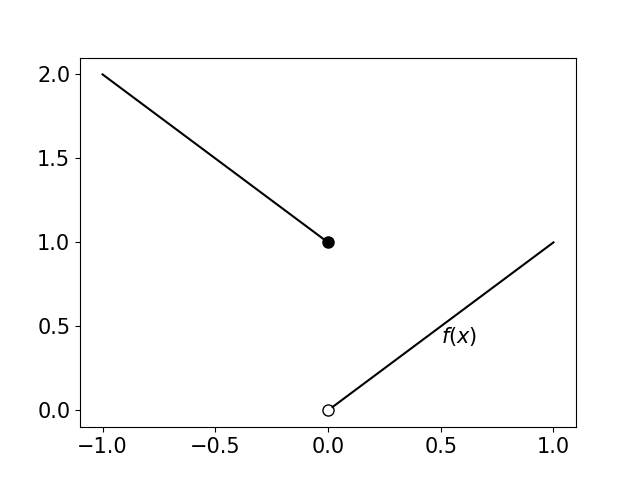
\includegraphics[width=0.4\textwidth]{figures/discontinuous_function.png}};
        \node at (7,0)
        {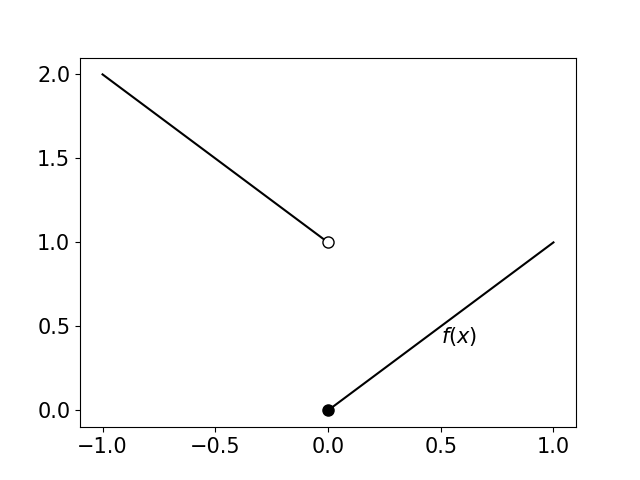
\includegraphics[width=0.4\textwidth]{figures/lsc_function.png}};
        \node at (0,-3) {Minimum tidak tercapai};
        \node at (7,-3) {Minimum tercapai};
    \end{tikzpicture}
    \caption{Kegagalan semikontinuitas bawah dapat menyebabkan infimum tidak
    tercapai.}
    \label{prelim:fig:lsc}
\end{figure}

\noindent\textbf{Deskripsi gambar.} Kedua panel menampilkan fungsi sepotong-sepotong
yang mempunyai lompatan di $x=0$. Pada panel kiri, cabang kanan mendekati titik
kosong $(0,0)$ sementara nilai fungsi di $x=0$ adalah titik penuh $(0,1)$;
infimum $0$ tidak tercapai. Pada panel kanan, titik $(0,0)$ diisi dan titik
$(0,1)$ dibiarkan kosong, sehingga nilai minimum $0$ tercapai.

% H01-S008 | sumber authority/habring/source-v1/preliminaries.tex baris 496--530
% segment-id: d90.hab.v1.ch01.seg0008
\begin{defn}[Koersif]
    Fungsi $f:V\rightarrow(-\infty,+\infty]$ disebut koersif jika
    \begin{equation}
        \lim_{\|x\|\rightarrow\infty}f(x)=\infty.
    \end{equation}
\end{defn}

\begin{theorem}\label{preliminaries:thm:direct_method}
    Misalkan $V$ berdimensi hingga dan
    $f:V\rightarrow(-\infty,\infty]$ proper, koersif, serta semikontinu bawah.
    Maka $f$ mencapai minimumnya pada $V$.\footnote{Asumsi dimensi hingga
    menyediakan kekompakan sekuensial yang dipakai bukti ini. Generalisasi ke
    dimensi tak hingga memerlukan hipotesis tambahan, misalnya refleksivitas dan
    semikontinuitas bawah lemah; ketiga asumsi yang ditampilkan saja tidak cukup.}
\end{theorem}

\begin{proof}
    Bukti mengikuti apa yang disebut \emph{metode langsung}.

    \paragraph{Langkah 1: Ambil barisan peminimum.}
    Misalkan $(x_n)_n$ suatu barisan peminimum\footnote{Sebagai latihan:
    mengapa barisan seperti ini selalu ada?}, yaitu
    \begin{equation}
        \lim_n f(x_n)=\inf_{x\in V}f(x).
    \end{equation}

    \paragraph{Langkah 2: Tunjukkan keterbatasan barisan.}
    Karena $f$ koersif, barisan peminimum harus terbatas. Jika tidak, terdapat
    subbarisan $(x_{n(k)})_k$ dengan $\|x_{n(k)}\|\rightarrow\infty$.
    Koersivitas kemudian memberikan
    \begin{equation}
        f(x_{n(k)})\rightarrow\infty,
    \end{equation}
    yang bertentangan dengan
    \begin{equation}
        f(x_{n(k)})\rightarrow\inf f<\infty.
    \end{equation}

    \paragraph{Langkah 3: Gunakan kekompakan untuk mengambil subbarisan
    konvergen.}
    Berdasarkan~\cref{thm:bolzano}, setiap barisan terbatas dalam ruang vektor
    berdimensi hingga mempunyai subbarisan konvergen. Jadi kita dapat mengambil
    subbarisan $(x_{n(k)})_k$ dengan limit
    $\lim_kx_{n(k)}=\hat x$.

    \paragraph{Langkah 4: Simpulkan dengan semikontinuitas bawah.}
    Berdasarkan semikontinuitas bawah $f$,
    \begin{equation}
        f(\hat x)
        \leq\liminf_{k\rightarrow\infty}f(x_{n(k)})
        =\lim_n f(x_n)
        =\inf_x f(x)
        \leq f(\hat x).
    \end{equation}
    Jadi semua ketaksamaan merupakan kesamaan dan $\hat x$ adalah peminim.
\end{proof}

\chapter{Kekonveksan}

% H02-S001 | sumber authority/habring/source-v1/convexity.tex baris 1--40
% segment-id: d90.hab.v1.ch02.seg0001
Tujuan kita dalam kuliah ini adalah menyelesaikan masalah berbentuk
\begin{equation}
    \min_{x\in C} f(x),
\end{equation}
dengan $C\subset V$ suatu \emph{himpunan bagian konveks} dari ruang $V$ dan $f:C\rightarrow (-\infty,\infty]$ suatu \emph{fungsi konveks}. Oleh karena itu, pada bagian berikut kita menganalisis secara lebih terperinci arti tepat kekonveksan himpunan dan fungsi serta akibat yang dapat ditarik dari sifat-sifat tersebut.

\section{Himpunan konveks}
Suatu himpunan disebut konveks apabila, untuk setiap dua titik di dalamnya, seluruh ruas garis lurus yang menghubungkan kedua titik itu juga termuat di dalam himpunan tersebut. Secara lebih formal:
\begin{defn}
    Suatu himpunan $C\subset V$ disebut konveks jika dan hanya jika, untuk setiap $x,y\in C$ dan $\lambda\in (0,1)$, berlaku
    \begin{equation}
        \lambda x + (1-\lambda) y\in C.
    \end{equation}
\end{defn}

Perhatikan bahwa
\begin{equation}
    \lambda x + (1-\lambda) y = y + \lambda(x-y),
\end{equation}
yang memperlihatkan dengan lebih jelas bahwa $\lambda x + (1-\lambda)y$ menelusuri ruas garis yang menghubungkan $x$ dan $y$.

Lebih lanjut, dengan menggunakan \emph{kombinasi konveks} yang lebih umum, kita dapat dengan mudah menunjukkan hasil berikut.

\begin{lemma}
    Himpunan $C\subset V$ konveks jika dan hanya jika, untuk setiap $n\in \N$, $x_i\in C$, dan $\lambda_i\in [0,1]$, $i=1,\dots,n$, yang memenuhi $\sum_{i=1}^n\lambda_i=1$, berlaku
    \begin{equation}
        \sum_{i=1}^n\lambda_i x_i \in C.
    \end{equation}
\end{lemma}
\begin{proof}
    Latihan.
\end{proof}

Untuk memudahkan notasi, kita mendefinisikan \emph{simpleks satuan} sebagai
\begin{equation}
    % Koreksi H02-C001 (sumber baris 37): batas penjumlahan n diganti k agar sesuai dengan Delta^k dan k komponen lambda.
    \Delta^k = \{(\lambda_1,\dots,\lambda_k)\in [0,1]^k\;|\;\sum_{i=1}^k\lambda_i = 1\}.
\end{equation}
Sekarang kita dapat mendefinisikan himpunan konveks terkecil yang memuat suatu himpunan, yaitu \emph{selubung konveks}.

% H02-S002 | sumber authority/habring/source-v1/convexity.tex baris 42--65
% segment-id: d90.hab.v1.ch02.seg0002
\begin{defn}[Selubung konveks]
    Misalkan $C\subset V$. Selubung konveks dari $C$ didefinisikan sebagai himpunan
    \begin{equation}\label{eq:convex_sets:defin_conv_hull}
        \conv(C) \coloneqq \bigcap_{\substack{S\subset V \text{ konveks}\\C\subset S}}S.
    \end{equation}
\end{defn}

\begin{lemma}
    Berlaku
    \begin{equation}\label{eq:convex_sets:conv_hull}
        % Koreksi H02-C028: vektor bobot ditulis lengkap, bukan skalar lambda.
        \conv(C) = \bigg\{ \sum_{i=1}^n\lambda_i x_i\;|\; n\in \N,\;x_i\in C, \;
        (\lambda_1,\ldots,\lambda_n)\in \Delta^n\bigg\}.
    \end{equation}
\end{lemma}
\begin{proof}
    Nyatakan ruas kanan \eqref{eq:convex_sets:conv_hull} dengan $A$.
    Kita akan menunjukkan bahwa $\conv(C)\subset A$ dan $A\subset\conv(C)$.

    \underline{$A\subset\conv(C)$:}
    Misalkan $x=\sum_{i=1}^n\lambda_i x_i\in A$. Untuk setiap $S\subset V$ yang konveks dan memenuhi $C\subset S$, berlaku $x\in S$. Oleh karena itu, berdasarkan definisi pada \eqref{eq:convex_sets:defin_conv_hull}, diperoleh $x\in\conv(C)$.

    \underline{$\conv(C)\subset A$:}
    Dapat diperiksa langsung bahwa $A$ memang merupakan himpunan konveks. Selain itu, $C\subset A$. Dengan demikian, $A$ termasuk salah satu himpunan $S$ dalam \eqref{eq:convex_sets:defin_conv_hull}, sehingga $\conv(C)\subset A$.
\end{proof}

% H02-S003 | sumber authority/habring/source-v1/convexity.tex baris 67--97
% segment-id: d90.hab.v1.ch02.seg0003
\begin{figure}
    \centering
    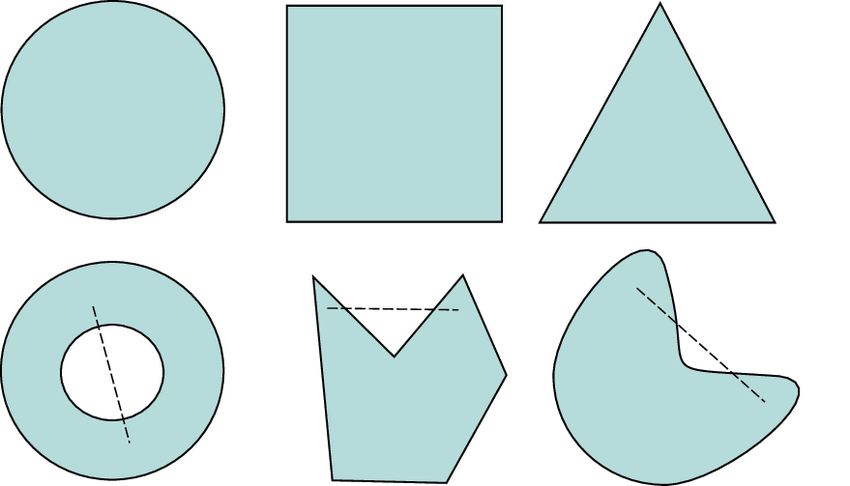
\includegraphics[width=.7\textwidth]{figures/sets.png}
    \caption{Baris atas: himpunan konveks. Baris bawah: himpunan tak konveks.}
\end{figure}

\noindent\textbf{Deskripsi gambar.} Baris atas memperlihatkan beberapa daerah yang memuat seluruh ruas garis di antara setiap dua titik di dalamnya. Baris bawah memperlihatkan daerah yang memiliki lekukan atau bagian terpisah sehingga terdapat dua titik di dalam himpunan yang ruas penghubungnya keluar dari himpunan.

\begin{example}
    Himpunan-himpunan berikut bersifat konveks (buktinya ditinggalkan sebagai latihan):
    \begin{itemize}
        \item Himpunan kosong $\emptyset$.
        \item Setiap ruang vektor.
        \item Setiap bola norma; yaitu, untuk setiap norma $\|\emptyarg\|$, setiap $c\in V$, dan setiap $R\geq 0$, himpunan
        \begin{equation}
            % Koreksi H02-C002 (sumber baris 80--82): tanda sama dengan yang hilang ditambahkan.
            B_{\|\emptyarg\|,R}(c)=\{x\in V\;|\; \|x-c\|<R\}
        \end{equation}
        dan
        \begin{equation}
            % Koreksi H02-C003 (sumber baris 84--86): tanda sama dengan yang hilang ditambahkan.
            \overline{B}_{\|\emptyarg\|,R}(c)=\{x\in V\;|\; \|x-c\|\leq R\}.
        \end{equation}
        \item Setiap subruang afin; yaitu, untuk setiap vektor $z,x_1,\dots,x_k\in V$, himpunan
        \begin{equation}
            \bigg\{ x\in V\;|\; x = z + \sum_{i=1}^k\lambda_i x_i,\; \lambda_i\in \R \bigg\}.
        \end{equation}
    \end{itemize}
\end{example}

\begin{figure}
    \centering
    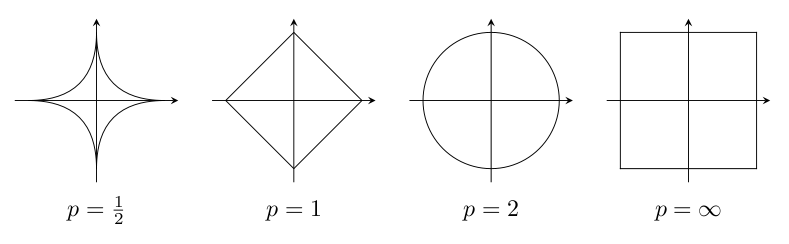
\includegraphics[width=1\textwidth]{figures/balls.png}
    \caption{Bola norma $\overline{B}_{\|\emptyarg\|_p,R}(0)$ untuk beberapa norma $\ell^p$. Perhatikan bahwa himpunan untuk $p=1/2$ tidak konveks karena pilihan ini tidak menghasilkan norma: ketaksamaan segitiga tidak berlaku.}
\end{figure}

\noindent\textbf{Deskripsi gambar.} Gambar membandingkan bola satuan dua dimensi untuk beberapa nilai $p$. Bentuknya berubah dari belah ketupat melalui lingkaran menuju bentuk yang semakin menyerupai persegi ketika $p$ bertambah; untuk $p=1/2$, sisi-sisinya melengkung ke dalam sehingga himpunannya tidak konveks.

% H02-S004 | sumber authority/habring/source-v1/convexity.tex baris 99--126
% segment-id: d90.hab.v1.ch02.seg0004
\begin{lemma}[Operasi yang mempertahankan kekonveksan]\label{convexity:lemma:ops preserving convexity}
    Pernyataan-pernyataan berikut berlaku:
    \begin{enumerate}
        \item Irisan. Misalkan $C_i\subset V$ konveks untuk $i\in I$, dengan $I$ suatu himpunan indeks sembarang. Maka irisan
        \begin{equation}
            \bigcap_{i\in I} C_i \coloneqq \{x\in V\;|\; x\in C_i\; \forall i\in I\}
        \end{equation}
        bersifat konveks.
        \item Jumlah berbobot. Misalkan $C_i\subset V$ konveks untuk $i=1,\dots,N$, dan misalkan $\lambda_i\in\R$ untuk $i=1,\dots,N$. Maka himpunan
        \begin{equation}
            % Koreksi H02-C004 (sumber baris 108--110): n dan indeks I yang tidak didefinisikan diseragamkan menjadi N dan i=1,...,N.
            \sum_{i=1}^N \lambda_i C_i \coloneqq \bigg\{\sum_{i=1}^N \lambda_i x_i\;|\; x_i\in C_i\; \forall i=1,\dots,N\bigg\}
        \end{equation}
        bersifat konveks.
        \item Produk Kartesius. Misalkan $C_i\subset V$ konveks untuk $i\in I$, dengan $I$ suatu himpunan indeks sembarang. Maka produk Kartesius
        \begin{equation}
            % Koreksi H02-C029: produk Kartesius memakai simbol produk, bukan produk tensor.
            \prod_{i\in I} C_i \coloneqq \{(x_i)_{i\in I}\;|\; x_i\in C_i\; \forall i\in I\}
        \end{equation}
        bersifat konveks.
        \item Citra dan pracitra\footnote{Pracitra terdefinisi dengan baik juga untuk pemetaan yang tidak invertibel.} di bawah pemetaan linear bersifat konveks. Secara khusus, untuk $A:V\rightarrow W$ linear serta $S\subset V$ dan $T\subset W$ keduanya konveks, himpunan-himpunan berikut bersifat konveks:
        \begin{equation}
            % Koreksi H02-C005 (sumber baris 120--122): pracitra diberi argumen T dan variabel himpunannya diperbaiki dari y menjadi x.
            A(S)=\{Ax\;|\;x\in S\},\qquad A^{-1}(T)=\{x\in V\;|\;Ax\in T\}.
        \end{equation}
    \end{enumerate}
\end{lemma}
\begin{proof}
    Kita hanya membuktikan bagian pertama dan meninggalkan sisanya sebagai latihan. Buktinya langsung. Misalkan $x,y\in\bigcap_{i\in I}C_i$ dan $\lambda\in(0,1)$. Karena $x,y\in C_i$ untuk setiap $i$ dan setiap $C_i$ konveks, diperoleh $\lambda x+(1-\lambda)y\in C_i$ untuk setiap $i$. Dengan demikian, $\lambda x+(1-\lambda)y\in\bigcap_{i\in I}C_i$.
\end{proof}

% H02-S005 | sumber authority/habring/source-v1/convexity.tex baris 128--191
% segment-id: d90.hab.v1.ch02.seg0005
Kita hendak mendefinisikan secara formal pengertian hiperbidang, yaitu perumuman bidang dua dimensi di $\R^3$ ke dimensi sembarang.

\begin{defn}[Hiperbidang]
    Misalkan $V$ suatu ruang hasil kali dalam. Hiperbidang adalah himpunan $H$ berbentuk
    \begin{equation}
        H=\{x\in V\;|\;\inner{x}{a}=b\}
    \end{equation}
    untuk suatu $a\in V\setminus\{0\}$ dan $b\in\R$.
\end{defn}

Parameter $a$ menentukan orientasi bidang dan $b$ menentukan geserannya. Secara khusus, $0\in H$ jika dan hanya jika $b=0$; dalam kasus ini $H$ merupakan subruang. Jika $b\neq0$, $H$ hanya merupakan subruang afin.

Perhatikan bahwa jika $x_0\in H$, maka
\begin{equation}
    H=\{x\in V\;|\;\inner{x-x_0}{a}=0\}.
\end{equation}
Jadi, $a$ adalah vektor normal terhadap bidang tersebut. Selain itu, dapat diperiksa sebagai latihan bahwa $\frac{|b|}{\|a\|}$ adalah jarak bidang dari titik asal.

Setiap hiperbidang membagi ruang menjadi dua setengah ruang.
\begin{defn}[Setengah ruang]
    Misalkan $V$ suatu ruang hasil kali dalam. Setengah ruang adalah himpunan $H^-$ berbentuk
    \begin{equation}
        H^-=\{x\in V\;|\;\inner{x}{a}\leq b\}
    \end{equation}
    untuk suatu $a\in V\setminus\{0\}$ dan $b\in\R$.
\end{defn}

Teorema berikut menyatakan bahwa pemisahan tersebut dapat dipilih dengan cara tertentu. Hasil ini ternyata sangat penting dalam optimisasi dan analisis fungsional.

\begin{theorem}[Teorema pemisahan Hahn--Banach]
    % Koreksi H02-C006 (sumber baris 156--166): ruang topologis, fungsional kontinu, dan ambang alpha yang semula dideklarasikan tetapi tidak dipakai dibuat eksplisit.
    Misalkan $S,T$ dua himpunan bagian konveks yang tak kosong dan saling lepas dari suatu ruang bernorma real $V$, dan misalkan $S$ terbuka. Maka terdapat $a\in V^*$ yang kontinu dan tak nol serta $\alpha\in\R$ sedemikian sehingga
    \begin{equation}
        \langle a,x\rangle<\alpha\leq\langle a,y\rangle,\qquad x\in S,\;y\in T.
    \end{equation}
    Jika $S$ dan $T$ keduanya tertutup dan salah satunya kompak, maka terdapat $a\in V^*$ yang kontinu dan tak nol, $\alpha\in\R$, dan $\epsilon>0$ sedemikian sehingga
    \begin{equation}
        \langle a,x\rangle\leq\alpha<\alpha+\epsilon\leq\langle a,y\rangle,\qquad x\in S,\;y\in T.
    \end{equation}
\end{theorem}
Versi kedua memungkinkan kita memperoleh selisih positif tegas antara
\[
    \sup_{x\in S}\langle a,x\rangle
    \quad
    \text{dan}
    \quad
    \inf_{y\in T}\langle a,y\rangle.
\]

\begin{figure}
    \centering
            \begin{tikzpicture}[font=\sffamily]
                \draw[dashed] (-2.5,3) -- (2.5,-0.5);
                \node[circle,draw,fill=gray,minimum size=2.4cm] at (1,2.4) {$S$};
                \draw[fill=gray,rounded corners] (-2,2) -- (-0.2,1) -- (0.2,-1) -- (-1.5,0) -- (-2.2,1.5) --cycle;
                \path (-2,2) --  (0.2,-1)  node[midway] {$T$};
                \draw[ultra thin] (-3,0) -- (3,0) (0,-2) -- (0,4);
            \end{tikzpicture}\hfill%
            \begin{tikzpicture}[font=\sffamily]
                \node[circle,draw,fill=gray,minimum size=2.4cm] at (1,2.4) {$S$};
                \draw[fill=gray,rounded corners] (0,4) -- (-0.5,1) -- (.5,.8) -- (2,.5) -- (0,-.5) -- (-1.5,0) -- (-2.2,1.5) --cycle;
                \path (-2,2) --  (0.2,-1)  node[midway] {$T$};
                \draw[ultra thin] (-3,0) -- (3,0) (0,-2) -- (0,4);
            \end{tikzpicture}
    \caption{Ilustrasi teorema pemisahan Hahn--Banach dan alasan pemisahan dapat gagal tanpa kekonveksan.}
\end{figure}

\noindent\textbf{Deskripsi gambar.} Panel kiri menampilkan dua himpunan konveks tak beririsan yang dipisahkan oleh sebuah garis putus-putus. Panel kanan menampilkan salah satu himpunan yang tak konveks dan melingkupi sebagian himpunan lainnya, sehingga tidak ada satu garis lurus yang dapat memisahkan keduanya.

\section{Fungsi konveks}

% H02-S006 | sumber authority/habring/source-v1/convexity.tex baris 193--261
% segment-id: d90.hab.v1.ch02.seg0006
Seperti diperlihatkan pada \cref{fig:convexity:1d_example}, kekonveksan sangat memengaruhi pertanyaan tentang keberadaan dan ketunggalan minimum.
\begin{figure}
    \centering
    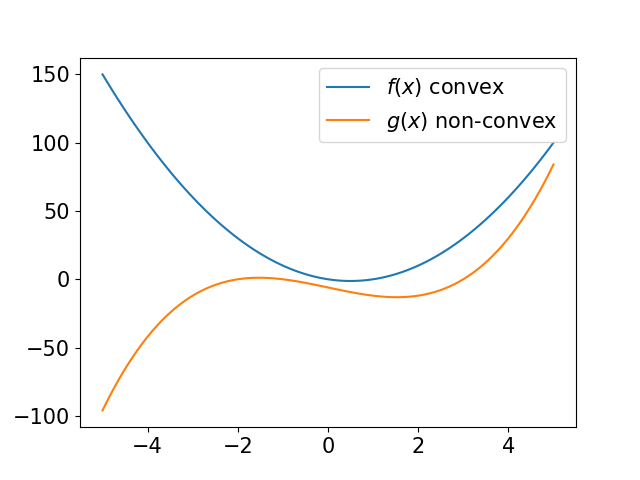
\includegraphics[width=0.5\textwidth]{figures/convex_fct.png}
    \caption{Contoh fungsi konveks dan fungsi tak konveks dalam satu dimensi.}
    \label{fig:convexity:1d_example}
\end{figure}

\noindent\textbf{Deskripsi gambar.} Gambar membandingkan grafik satu dimensi berbentuk mangkuk, yang konveks dan memiliki struktur minimum yang teratur, dengan grafik tak konveks yang memiliki lekukan serta beberapa minimum lokal.

\begin{defn}[Syarat orde nol untuk kekonveksan]
    Misalkan $C\subset V$ konveks dan $f:C\rightarrow(-\infty,\infty]$.
    \begin{itemize}
        \item Fungsi $f$ disebut konveks jika dan hanya jika, untuk setiap $x,y\in C$ dan $\lambda\in(0,1)$, berlaku
        \begin{equation}
            f(\lambda x+(1-\lambda)y)\leq\lambda f(x)+(1-\lambda)f(y).
        \end{equation}
        \item Fungsi $f$ disebut konveks tegas jika dan hanya jika, untuk setiap
        $x,y\in\dom(f)$ dengan $x\neq y$ dan setiap $\lambda\in(0,1)$, berlaku
        \begin{equation}
            % Koreksi H02-C007 (sumber baris 210--213): syarat x tidak sama dengan y ditambahkan; tanpa syarat ini ketaksamaan tegas mustahil saat x=y.
            f(\lambda x+(1-\lambda)y)<\lambda f(x)+(1-\lambda)f(y).
        \end{equation}
        \item Fungsi $f$ disebut konveks kuat dengan parameter $\mu>0$ jika dan
        hanya jika, untuk setiap $x,y\in\dom(f)$ dan $\lambda\in(0,1)$, berlaku
        % Koreksi H02-C025 (sumber baris 214): syarat mu>0 dibuat eksplisit; mu=0 hanya menghasilkan kekonveksan biasa.
        % Koreksi H02-C037: untuk fungsi nilai-diperluas, syarat tegas/kuat dibatasi pada domain efektif.
        \begin{equation}
            f(\lambda x+(1-\lambda)y)\leq\lambda f(x)+(1-\lambda)f(y)-\frac{\lambda(1-\lambda)\mu}{2}\|x-y\|^2.
        \end{equation}
    \end{itemize}
\end{defn}
Syarat orde nol menyatakan bahwa ruas garis yang menghubungkan dua titik pada grafik, yaitu garis sekan, selalu berada di atas fungsi. Untuk fungsi konveks tegas, garis sekan berada secara tegas di atas fungsi, sedangkan dalam kasus konveks kuat kita bahkan dapat \emph{menyisipkan} fungsi kuadrat di antara keduanya.

\begin{figure}
    \centering
    \begin{tikzpicture}[inner sep=.5mm,
            declare function={
                f(\x)= (\x-3)^2+3*\x-4;
            }
            ]
            \begin{axis}[axis lines=middle,domain=-1:4,samples=200,xtick={0.5,3},xticklabels={$x$,$y$},ytick=\empty,xmin=-.2,xmax=3.7,ymin=-.1,ymax=10]
                \addplot[blue,very thick,name path=f] {f(x)};
                \pgfplotsinvokeforeach{.5,3}{
                    \path[name path=x] (#1,0) -- (#1,6);
                    \draw[black!50,thick,dashed,name intersections={of=f and x, name=i}] (#1,0) -- (i-1);
                }
                \draw[very thick] ($(.5,{f(.5)})$) node[circle,fill=blue,label=left:{$f(x)$}]{} -- ($(3,{f(3)})$) node[circle,fill=blue,label=right:{$f(y)$}]{};
                \node[text=blue] at (1.75,2) {$f(\lambda x+(1-\lambda)y)$};
                \node[rotate=10] at (1.75,5) {$\lambda f(x)+(1-\lambda)f(y)$};
            \end{axis}
        \end{tikzpicture}
        \caption{Penafsiran geometris syarat orde nol bagi kekonveksan suatu fungsi.}
\end{figure}

\noindent\textbf{Deskripsi gambar.} Sebuah kurva konveks biru ditampilkan bersama dua titik pada grafik dan ruas sekan yang menghubungkannya. Nilai fungsi pada kombinasi konveks kedua titik berada di bawah nilai yang diperoleh melalui interpolasi linear di sepanjang sekan.

\begin{example}
    Fungsi-fungsi berikut konveks (bukti: latihan):
    \begin{enumerate}
        \item Fungsi afin $f(x)=\langle a,x\rangle+b$ dengan $a\in V^*$ dan $b\in\R$; khususnya, fungsi linear ketika $b=0$.
        % Koreksi H02-C008 (sumber baris 247): simbol y/a yang tidak konsisten diseragamkan menjadi a, dan koefisien dinyatakan sebagai fungsional linear a di V^*.
        \item Semua norma merupakan fungsi konveks.
    \end{enumerate}
\end{example}

Serupa dengan hasil untuk himpunan konveks, kekonveksan dapat diperluas ke kombinasi konveks dengan banyak titik yang sembarang.

\begin{theorem}[Jensen]
    % Koreksi H02-C026 (sumber baris 255): kodomain nilai-diperluas dibuat konsisten dan kasus bobot nol dinyatakan.
    Misalkan $C\subset V$ konveks dan
    $f:C\rightarrow(-\infty,+\infty]$. Dengan konvensi
    $0\cdot(+\infty)=0$, fungsi $f$ konveks jika dan hanya jika, untuk setiap
    $k\in\N$, $\lambda\in\Delta^k$, dan $x_i\in C$, berlaku
    \begin{equation}
        f\bigg(\sum_{i=1}^k\lambda_i x_i\bigg)\leq\sum_{i=1}^k\lambda_i f(x_i).
    \end{equation}
\end{theorem}

% H02-S007 | sumber authority/habring/source-v1/convexity.tex baris 262--322
% segment-id: d90.hab.v1.ch02.seg0007
Di atas kita melihat bahwa kekonveksan berarti garis sekan berada di atas fungsi. Kekonveksan juga berarti garis singgung berada di bawah fungsi (\cf~\cref{convexity:fig:gradients}).

\begin{theorem}[Karakterisasi orde pertama kekonveksan]\label{convexity:thm:first_order}
    % Koreksi H02-C030: turunan pada titik batas didefinisikan melalui perluasan ke lingkungan terbuka.
    Misalkan $C\subset\R^d$ konveks dan $f:C\rightarrow\R$ mempunyai perluasan
    yang terdiferensialkan secara kontinu pada suatu lingkungan terbuka dari $C$.
    \begin{itemize}
        \item Fungsi $f$ konveks jika dan hanya jika, untuk semua $x,y\in C$,
        \[
            f(x)+\langle\nabla f(x),y-x\rangle\leq f(y).
        \]
        \item Fungsi $f$ konveks tegas jika dan hanya jika ketaksamaan di atas berlaku tegas untuk semua $x\neq y$.
    \end{itemize}
\end{theorem}
\begin{proof}
    Kita terlebih dahulu membuktikan butir pertama.

    $\Rightarrow$: Misalkan $f$ konveks. Maka
    \begin{equation}
        f(x+\lambda(y-x))=f(\lambda y+(1-\lambda)x)\leq\lambda f(y)+(1-\lambda)f(x).
    \end{equation}
    Dengan menyusun ulang, diperoleh
    \begin{equation}
        \frac{f(x+\lambda(y-x))-f(x)}{\lambda}\leq f(y)-f(x).
    \end{equation}
    Membiarkan $\lambda\rightarrow0$ memberikan hasil yang diinginkan.

    $\Leftarrow$: Sekarang andaikan syarat gradien berlaku. Tuliskan $x_\lambda=x+\lambda(y-x)$. Maka
    \begin{equation*}
        f(x_\lambda)+\langle\nabla f(x_\lambda),y-x_\lambda\rangle
        =f(x_\lambda)+\langle\nabla f(x_\lambda),(1-\lambda)(y-x)\rangle\leq f(y)
    \end{equation*}
    dan
    \begin{equation*}
        f(x_\lambda)+\langle\nabla f(x_\lambda),x-x_\lambda\rangle
        =f(x_\lambda)+\langle\nabla f(x_\lambda),-\lambda(y-x)\rangle\leq f(x).
    \end{equation*}
    Kalikan ketaksamaan pertama dengan $\lambda$, ketaksamaan kedua dengan $1-\lambda$, lalu jumlahkan. Hasilnya
    \begin{equation*}
        f(x_\lambda)\leq\lambda f(y)+(1-\lambda)f(x).
    \end{equation*}

    % Koreksi H02-C036 (sumber baris 270 dan 273--274): bukti karakterisasi tegas yang hilang dilengkapi.
    Untuk butir kedua, arah dari syarat orde pertama tegas menuju kekonveksan
    tegas langsung mengikuti argumen yang sama. Sebaliknya, jika $f$ konveks
    tegas dan $x\neq y$, fungsi satu variabel
    $g(t)=f(x+t(y-x))$ konveks tegas pada $[0,1]$. Kemiringan sekan
    $(g(t)-g(0))/t$ tak menurun dalam $t>0$ dan, untuk setiap $t_0\in(0,1)$,
    bernilai tegas lebih kecil daripada $g(1)-g(0)$. Mengambil limit
    $t\downarrow0$ memberikan
    $\langle\nabla f(x),y-x\rangle< f(y)-f(x)$.
\end{proof}

\begin{figure}
    \centering
    \begin{tikzpicture}[inner sep=.5mm,
            declare function={
                f(\x)=  (\x-3)^2+3*\x-4;
            }
            ]
            \begin{axis}[axis lines=middle,domain=-1:4,samples=200,xtick={2},xticklabels={$x$},ytick=\empty,xmin=-.2,xmax=3.7,ymin=-.1,ymax=10]
                \addplot[blue,very thick,name path=f] {f(x)};
                \pgfplotsinvokeforeach{2}{
                    \path[name path=x] (#1,0) -- (#1,6);
                    \draw[black!50,thick,dashed,name intersections={of=f and x, name=i}] (#1,0) -- (i-1);
                }
                \addplot[very thick] {f(2)+1*(x-2)};
                \node[circle,fill=blue,label=above:{$f(x)$}] at ($(2,{f(2)})$) {};
                \node[text=blue,yshift=5mm] at ($(.5,{f(.5)})$) {$f$};
            \end{axis}
            \node[rotate=17,yshift=-3mm] at (6, 2.5) {$\textcolor{black}{y \mapsto f(x)+\inner{\nabla f(x)}{y-x}}$};
        \end{tikzpicture}
        \caption{Penafsiran geometris syarat orde pertama bagi fungsi konveks.}
        \label{convexity:fig:gradients}
\end{figure}

\noindent\textbf{Deskripsi gambar.} Grafik sebuah fungsi konveks ditampilkan bersama garis singgungnya pada titik $x$. Garis afin $y\mapsto f(x)+\langle\nabla f(x),y-x\rangle$ berada di bawah grafik fungsi di seluruh domain yang diperlihatkan.

% H02-S008 | sumber authority/habring/source-v1/convexity.tex baris 324--376
% segment-id: d90.hab.v1.ch02.seg0008
\begin{defn}[Minimum]
    % Koreksi H02-C021 (sumber baris 324--325): x^* dinyatakan berada di domain C.
    Misalkan $f:C\rightarrow\R$ dan $x^*\in C$.
    \begin{itemize}
        \item Titik $x^*$ disebut minimum lokal jika dan hanya jika terdapat $\epsilon>0$ sedemikian sehingga
        \[
            % Koreksi H02-C009 (sumber baris 328--330): pembanding dibatasi pada domain C.
            f(x^*)\leq f(x),\qquad \forall x\in B_\epsilon(x^*)\cap C.
        \]
        \item Titik $x^*$ disebut minimum global jika dan hanya jika
        \[
            f(x^*)\leq f(x),\qquad \forall x\in C.
        \]
    \end{itemize}
    Minimum disebut \emph{tegas} apabila ketaksamaan yang bersesuaian berlaku tegas untuk semua titik pembanding $x\neq x^*$.
    % Koreksi H02-C010 (sumber baris 336): pengecualian x=x^* dibuat eksplisit karena ketaksamaan tegas tidak mungkin berlaku di titik yang sama.
\end{defn}

Sekarang kita dapat membuktikan hasil penting pertama dalam optimisasi konveks.
\begin{prop}\label{convexity:prop:OC1}
    % Koreksi H02-C011 (sumber baris 340--342): asumsi bahwa f konveks ditambahkan; tanpa asumsi ini titik stasioner tidak harus menjadi minimum global.
    % Koreksi H02-C031: titik stasioner dinyatakan berada di domain dan hipotesis diferensial diselaraskan dengan teorema sebelumnya.
    Misalkan $C\subset\R^d$ konveks, $f:C\rightarrow\R$ konveks dan mempunyai
    perluasan yang terdiferensialkan secara kontinu pada suatu lingkungan
    terbuka dari $C$, serta $x^*\in C$. Jika $\nabla f(x^*)=0$, maka $x^*$
    adalah peminimum \textbf{global}.
\end{prop}
\begin{proof}
    Berdasarkan karakterisasi orde pertama kekonveksan,
    \begin{equation}
        f(x)\geq f(x^*)+\langle\nabla f(x^*),x-x^*\rangle
        =f(x^*)+0.
    \end{equation}
\end{proof}

Perhatikan bahwa kebalikan \cref{convexity:prop:OC1}, yaitu implikasi
\begin{equation}
    \text{$x^*$ adalah minimum}\Rightarrow\nabla f(x^*)=0,
\end{equation}
secara umum hanya benar apabila $x^*$ berada di interior $C$, yang dinyatakan dengan $C^\circ$; yaitu, terdapat $\epsilon>0$ sedemikian sehingga $B_\epsilon(x^*)\subset C$.

\begin{theorem}
    % Koreksi H02-C012 (sumber baris 357--359): domain Euklides dan asumsi kekonveksan f dibuat eksplisit agar ekuivalensi sah.
    Misalkan $C\subset\R^d$ konveks, $f:C\rightarrow\R$ konveks dan mempunyai
    perluasan yang terdiferensialkan secara kontinu pada suatu lingkungan
    terbuka dari $C$, serta $x^*\in C^\circ$. Maka $\nabla f(x^*)=0$ jika dan
    hanya jika $x^*$ adalah peminimum global.
\end{theorem}
\begin{proof}
    Satu arah mengikuti \cref{convexity:prop:OC1}. Untuk arah lainnya, andaikan $x^*$ suatu minimum. Untuk setiap $v\in\R^d$, jika $t>0$ cukup kecil, optimalitas memberikan
    \begin{equation}
        f(x^*+tv)-f(x^*)\geq0.
    \end{equation}
    Karena $t>0$, pembagian dengan $t$ menghasilkan
    \begin{equation}
        \frac{f(x^*+tv)-f(x^*)}{t}\geq0.
    \end{equation}
    Dengan membiarkan $t\rightarrow0$, diperoleh
    \begin{equation}
        \langle\nabla f(x^*),v\rangle\geq0.
    \end{equation}
    Karena $v$ sembarang, argumen yang sama dapat diterapkan pada $-v$. Hasilnya
    \[
        \langle\nabla f(x^*),v\rangle\leq0.
    \]

    Jadi $\langle\nabla f(x^*),v\rangle=0$ untuk setiap $v$, dan karenanya
    $\nabla f(x^*)=0$ (mengapa?).
\end{proof}

% H02-S009 | sumber authority/habring/source-v1/convexity.tex baris 378--403
% segment-id: d90.hab.v1.ch02.seg0009
Dalam satu dimensi, jika suatu fungsi terdiferensialkan, kekonveksannya dapat dikarakterisasi melalui kemonotonan turunannya. Dalam dimensi sembarang berlaku hasil berikut.

\begin{theorem}[Kemonotonan gradien]
    % Koreksi H02-C032: domain, perluasan diferensial, dan kuantifier x,y dibuat eksplisit.
    Misalkan $C\subset\R^d$ konveks dan $f:C\rightarrow\R$ mempunyai perluasan
    yang terdiferensialkan secara kontinu pada suatu lingkungan terbuka dari
    $C$. Maka $f$ konveks jika dan hanya jika, untuk setiap $x,y\in C$,
    \begin{equation}
        \langle\nabla f(x)-\nabla f(y),x-y\rangle\geq0.
    \end{equation}
\end{theorem}
\begin{proof}
    $\Rightarrow$: Andaikan $f$ konveks. Berdasarkan karakterisasi orde pertama kekonveksan,
    \begin{equation}
        \begin{aligned}
            &f(x)+\langle\nabla f(x),y-x\rangle\leq f(y),\\
            &f(y)+\langle\nabla f(y),x-y\rangle\leq f(x).
        \end{aligned}
    \end{equation}
    Menjumlahkan kedua ketaksamaan memberikan hasil yang diinginkan.

    $\Leftarrow$: Andaikan $\nabla f$ monoton. Berdasarkan teorema dasar kalkulus,
    \begin{equation}
        \begin{aligned}
            f(y)-f(x)
            &=\int_0^1\frac{\dd}{\dd t}f(x+t(y-x))\dd t\\
            &=\int_0^1\langle\nabla f(x+t(y-x)),y-x\rangle\dd t\\
            &=\int_0^1\langle\nabla f(x+t(y-x))-\nabla f(x),y-x\rangle\dd t+\langle\nabla f(x),y-x\rangle\\
            &=\int_0^1\frac{1}{t}\underbrace{\langle\nabla f(x+t(y-x))-\nabla f(x),t(y-x)\rangle}_{\geq0}\dd t+\langle\nabla f(x),y-x\rangle\\
            &\geq\langle\nabla f(x),y-x\rangle.
        \end{aligned}
    \end{equation}
    Pada $t=0$, integran dipahami melalui perpanjangan kontinu; ketaksamaan monoton digunakan untuk $t\in(0,1]$.
\end{proof}

% H02-S010 | sumber authority/habring/source-v1/convexity.tex baris 405--453
% segment-id: d90.hab.v1.ch02.seg0010
Terakhir, turunan kedua juga dapat digunakan untuk mengarakterisasi kekonveksan. Secara intuitif, kekonveksan berarti \emph{kelengkungan positif}. Untuk memformalkan hal ini, ingat kembali cara mengurutkan matriks. Untuk dua matriks simetris $A,B\in\R^{d\times d}$, kita menuliskan
    % Koreksi H02-C022 (sumber baris 407--414): A dan B dinyatakan simetris karena urutan Loewner digunakan pada matriks simetris.
\begin{equation}
    A\succeq B\Longleftrightarrow\langle x,Ax\rangle\geq\langle x,Bx\rangle,\quad\forall x\in\R^d
\end{equation}
dan, serupa dengan itu,
\begin{equation}
    % Koreksi H02-C013 (sumber baris 411--413): x=0 dikecualikan dari urutan positif tegas.
    A\succ B\Longleftrightarrow\langle x,Ax\rangle>\langle x,Bx\rangle,\quad\forall x\in\R^d\setminus\{0\}.
\end{equation}

\begin{theorem}[Karakterisasi orde kedua kekonveksan]
    % Koreksi H02-C027 (sumber baris 416--417): C dinyatakan terbuka di R^d; tanpa domain berdimensi penuh, Hessian pada arah normal tidak mengarakterisasi kekonveksan restriksi.
    Misalkan $C\subset\R^d$ terbuka dan konveks, serta $f:C\rightarrow\R$ terdiferensialkan secara kontinu dua kali.
    \begin{enumerate}
        \item Fungsi $f$ konveks jika dan hanya jika $\nabla^2f(x)\succeq0$ untuk setiap $x\in C$.
        \item Jika $\nabla^2f(x)\succ0$ untuk setiap $x\in C$, maka $f$ konveks tegas.
        % Koreksi H02-C014 (sumber baris 420): ekuivalensi yang salah diganti dengan implikasi; fungsi x^4 konveks tegas tetapi Hessian-nya nol di x=0.
    \end{enumerate}
\end{theorem}
\begin{proof}
    Kita membuktikan pernyataan pertama dan arah cukup pada pernyataan kedua.

    $\Rightarrow$: Andaikan $f$ konveks. Berdasarkan kemonotonan gradien, untuk $t>0$ berlaku
    \begin{equation}
        \frac{\inner{\nabla f(x+tv)-\nabla f(x)}{v}}{t}\geq0.
    \end{equation}
    Dengan membiarkan $t\rightarrow0$, diperoleh
    \begin{equation}
        \langle v,\nabla^2f(x)v\rangle\geq0.
    \end{equation}
    Karena $v$ sembarang, hasilnya mengikuti.

    $\Leftarrow$: Andaikan $\nabla^2f\succeq0$. Berdasarkan teorema dasar kalkulus,
    \begin{equation}
        \begin{aligned}
            \nabla f(y)-\nabla f(x)
            &=\int_0^1\frac{\dd}{\dd t}\nabla f(x+t(y-x))\dd t\\
            &=\int_0^1\nabla^2f(x+t(y-x))(y-x)\dd t.
        \end{aligned}
    \end{equation}
    Mengambil hasil kali dalam dengan $y-x$ menghasilkan
    \begin{equation}
        \begin{aligned}
            % Koreksi H02-C015 (sumber baris 444--449): integran vektor yang salah pada ruas kanan diganti dengan bentuk kuadratik skalar.
            \langle\nabla f(y)-\nabla f(x),y-x\rangle
            &=\int_0^1\underbrace{\langle y-x,\nabla^2f(x+t(y-x))(y-x)\rangle}_{\geq0}\dd t\\
            &\geq0.
        \end{aligned}
    \end{equation}
    Kemonotonan gradien kini menyiratkan kekonveksan. Untuk membuktikan bagian
    tegas, tuliskan $d=y-x\neq0$. Jika Hessian positif definit pada setiap titik,
    maka
    \[
        f(y)-f(x)-\langle\nabla f(x),d\rangle
        =\int_0^1\int_0^t
        \langle d,\nabla^2f(x+sd)d\rangle\,\dd s\,\dd t>0.
    \]
    Jadi ketaksamaan orde pertama berlaku tegas dan $f$ konveks tegas.
\end{proof}

% \subsubsection{Operasi yang mempertahankan kekonveksan}

% H02-S011 | sumber authority/habring/source-v1/convexity.tex baris 457--484
% segment-id: d90.hab.v1.ch02.seg0011
\begin{lemma}[Operasi yang mempertahankan kekonveksan]
    Misalkan $f,f_1,\dots,f_n:C\rightarrow\R$ konveks pada suatu himpunan konveks.
    \begin{enumerate}
        \item Untuk setiap $\alpha\geq0$, fungsi $\alpha f$ konveks.
        \item Fungsi $\sum_i f_i$ konveks.
    \end{enumerate}
\end{lemma}
\begin{proof}
    Latihan.
\end{proof}

\begin{lemma}[Operasi yang mempertahankan kekonveksan, lanjutan]
    Misalkan $f:\R^n\supset C\rightarrow\R$ konveks, $A\in\R^{n\times m}$, dan $b\in\R^n$. Maka
    \begin{equation}
        g(x)=f(Ax+b)
    \end{equation}
    konveks pada $\{x\in\R^m\;|\;Ax+b\in C\}$.
\end{lemma}
\begin{proof}
    Latihan.
\end{proof}

\begin{lemma}[Operasi yang mempertahankan kekonveksan, lanjutan]
    Misalkan $f:C\rightarrow\R$ konveks dan $g:I\rightarrow\R$ konveks serta tak menurun, dengan $I\subset\R$ suatu interval yang memenuhi $f(C)\subset I$. Maka $g\circ f$ konveks.
\end{lemma}
\begin{proof}
    Latihan.
\end{proof}

% H02-S012 | sumber authority/habring/source-v1/convexity.tex baris 486--543
% segment-id: d90.hab.v1.ch02.seg0012
\begin{example}
    \begin{enumerate}
        \item Fungsi \emph{log-sum-exp} bersifat konveks:
        \begin{equation}
            f(x)=\log\bigg(\sum_{i=1}^n e^{x_i}\bigg).
        \end{equation}
        \item Fungsi kuadratik-per-linear
        \begin{equation}
            f(x)=\frac{x_1^2}{x_2}
        \end{equation}
        konveks pada $\R\times(0,\infty)$.
        \item Fungsi $h(x)=e^{\|x\|^2}$ konveks pada $\R^d$ karena $f(x)=\|x\|^2$ konveks dan $g(t)=e^t$ konveks serta tak menurun.
        \item Pertimbangkan $h(x)=(\|x\|^2+1)^2$ pada $\R^d$. Fungsi $f(x)=\|x\|^2+1$ dan $g(t)=t^2$ keduanya konveks. Fungsi $g$ tidak tak menurun pada seluruh $\R$, tetapi tak menurun pada $f(\R^d)=[1,\infty)$. Akibatnya, $h$ konveks.
        \item Pada contoh sebelumnya, jika $f$ diganti dengan $\|\emptyarg\|^2-1$, maka $g$ tidak tak menurun pada $f(\R^d)=[-1,\infty)$; lihat \cref{convexity:fig:compositions}.
        % Koreksi H02-C033: dimensi domain fungsi diseragamkan dari n menjadi d.
    \end{enumerate}
\end{example}

\begin{figure}
    \centering
    \begin{tikzpicture}[declare function={
            f1(\x) =  \x^2 + 1;
            f2(\x) =  \x^2 - 1;
            g(\x) = \x^2;
            h1(\x) = g(f1(\x));
            h2(\x) = g(f2(\x));
        }
        ]
        \begin{groupplot}[
            group style={group size= 3 by 1,vertical sep=1.5cm}, height=4.5cm, width=5.3cm,ymin=-1.2,ymax=2.5,domain=-2:2,xmin=-1.6,xmax=1.6,samples=200,grid
        ]
            \nextgroupplot[
                align=center,
                title={%
                    \( \textcolor{teal}{f_1 : x \mapsto x^2 + 1} \) \\
                    \( \textcolor{red}{f_2 : x \mapsto x^2 - 1} \)
                }
            ]
                \addplot[teal, very thick] {f1(x)};
                \addplot[red, very thick] {f2(x)};
            \nextgroupplot[title={\( g : x \mapsto x^2\)}]
                \draw[->, teal, very thick] (axis cs:1, 0) -- (axis cs:1.5, 0) node [midway, above] {\( \textcolor{teal}{f_1(\R)} \)};
                \draw[->, red, very thick] (axis cs:-1, 0) -- (axis cs:.5, 0) node [midway, below] {\( \textcolor{red}{f_2(\R)} \)};
                \addplot[blue, very thick] {g(x)};
            \nextgroupplot[
                align=center,
                title={%
                    \( \textcolor{teal}{g \circ f_1 } \) \\
                    \( \textcolor{red}{g \circ f_2 } \)
                }
            ]
                \addplot[teal, very thick] {h1(x)};
                \addplot[red, very thick] {h2(x)};
        \end{groupplot}
    \end{tikzpicture}
    \caption{Kekonveksan komposisi fungsi.}
    \label{convexity:fig:compositions}
\end{figure}

\noindent\textbf{Deskripsi gambar.} Panel kiri menampilkan $f_1(x)=x^2+1$ dan $f_2(x)=x^2-1$. Panel tengah menampilkan $g(t)=t^2$ serta rentang kedua fungsi tersebut; $g$ tak menurun pada rentang $f_1$ tetapi tidak pada seluruh rentang $f_2$. Panel kanan memperlihatkan bahwa $g\circ f_1$ konveks, sedangkan $g\circ f_2$ memiliki lekukan tak konveks di sekitar titik asal.

% H02-S013 | sumber authority/habring/source-v1/convexity.tex baris 545--564
% segment-id: d90.hab.v1.ch02.seg0013
\begin{lemma}[Operasi yang mempertahankan kekonveksan, lanjutan]
    Misalkan $f_i:C\rightarrow\R$, $i=1,\dots,n$, konveks pada himpunan konveks $C$. Maka
    \begin{equation}
        f(x)=\max_{i=1,\dots,n}f_i(x)
    \end{equation}
    konveks.
\end{lemma}
\begin{proof}
    Kita hitung langsung:
    \begin{equation}
        \begin{aligned}
            f(\lambda x+(1-\lambda)y)
            &=\max_i f_i(\lambda x+(1-\lambda)y)\\
            &\leq\max_i\{\lambda f_i(x)+(1-\lambda)f_i(y)\}\\
            &\leq\lambda\max_jf_j(x)+(1-\lambda)\max_jf_j(y)\\
            &=\lambda f(x)+(1-\lambda)f(y).
        \end{aligned}
    \end{equation}
\end{proof}

% H02-S014 | sumber authority/habring/source-v1/convexity.tex baris 566--596
% segment-id: d90.hab.v1.ch02.seg0014
\begin{theorem}\label{convexity:thm:minimum}
    Misalkan $f:C\times D\rightarrow\R$ konveks pada $C\times D$, dengan $C$ dan $D$ keduanya konveks. Definisikan
    \begin{equation}
        g(x)=\inf_{y\in D}f(x,y),
    \end{equation}
    dan andaikan infimum tersebut hingga untuk setiap $x\in C$. Maka $g$ konveks.
\end{theorem}
\begin{proof}
    Pilih barisan $y_n^x$ dan $y_n^z$ sedemikian sehingga
    \begin{equation}
        g(x)=\lim_n f(x,y_n^x),\qquad g(z)=\lim_n f(z,y_n^z).
    \end{equation}
    Maka
    \begin{equation}
        \begin{aligned}
            g(\lambda x+(1-\lambda)z)
            &\leq f(\lambda x+(1-\lambda)z,\lambda y_n^x+(1-\lambda)y_n^z)\\
            &\leq\lambda f(x,y_n^x)+(1-\lambda)f(z,y_n^z).
        \end{aligned}
    \end{equation}
    Mengambil limit ketika $n\rightarrow\infty$ menyelesaikan bukti.
\end{proof}

\begin{example}
    % Koreksi H02-C016 (sumber baris 589--595): C harus tak kosong dan konveks; jarak ke himpunan tak konveks tidak selalu konveks.
    Jarak suatu titik ke himpunan tak kosong dan konveks merupakan fungsi konveks. Jadi, untuk setiap himpunan tak kosong dan konveks $C\subset\R^d$, pemetaan berikut konveks:
    \begin{equation}
        \begin{aligned}
            x\mapsto d(x,C)\coloneqq\inf_{y\in C}\|x-y\|.
        \end{aligned}
    \end{equation}
\end{example}

% H02-S015 | sumber authority/habring/source-v1/convexity.tex baris 598--624
% segment-id: d90.hab.v1.ch02.seg0015
\begin{theorem}
    % Koreksi H02-C017 (sumber baris 598--606): klausa g konveks dan domain garis yang berada di C ditambahkan; rumus sumber berakhir tanpa predikat dan memakai seluruh R walau x+tv dapat keluar dari C.
    Misalkan $C\subset\R^d$ konveks dan $f:C\rightarrow\R$. Maka $f$ konveks jika dan hanya jika, untuk setiap $x\in C$ dan $v\in\R^d$, fungsi
    \begin{equation}
        \begin{aligned}
            g:I_{x,v}&\rightarrow\R,\\
            t&\mapsto g(t)=f(x+tv),
        \end{aligned}
    \end{equation}
    konveks pada interval $I_{x,v}\coloneqq\{t\in\R\mid x+tv\in C\}$.
\end{theorem}
\begin{proof}
    $\Leftarrow$: Andaikan $g$ konveks untuk setiap $x$ dan $v$. Misalkan $x,y\in C$ dan $\lambda\in(0,1)$. Pertimbangkan
    \begin{equation}
        g(t)=f(y+t(x-y)).
    \end{equation}
    Karena $g$ konveks pada interval yang memuat $0$ dan $1$,
    \begin{equation}
        \begin{aligned}
            f(\lambda x+(1-\lambda)y)
            =g(\lambda)
            &=g(\lambda\cdot1+(1-\lambda)\cdot0)\\
            &\leq\lambda g(1)+(1-\lambda)g(0)\\
            &=\lambda f(x)+(1-\lambda)f(y).
        \end{aligned}
    \end{equation}
    Arah sebaliknya ditinggalkan sebagai latihan.
\end{proof}

% H02-S016 | sumber authority/habring/source-v1/convexity.tex baris 626--681
% segment-id: d90.hab.v1.ch02.seg0016
\begin{example}[Fungsi konveks yang umum]
    % Koreksi H02-C023 (sumber baris 626): garis miring terbalik yatim setelah pembuka lingkungan example dihapus.
    \begin{itemize}
        \item Contoh pada $\R$:
        \begin{itemize}
            \item Fungsi konveks:
            \begin{itemize}
                \item Fungsi eksponensial $f(x)=\exp(ax)$ pada $\R$, dengan $a\in\R$.
                \item Fungsi pangkat $f(x)=x^p$ pada $(0,\infty)$ untuk $p\geq1$ atau $p\leq0$.
                \item Pangkat nilai mutlak $f(x)=|x|^p$ pada $\R$ untuk $p\geq1$.
                \item Entropi negatif $f(x)=x\log(x)$ pada $(0,\infty)$.
            \end{itemize}
            \item Fungsi konkaf:
            \begin{itemize}
                \item Fungsi pangkat $f(x)=x^p$ pada $(0,\infty)$ untuk $0\leq p\leq1$.
                \item Logaritma $f(x)=\log(x)$ pada $(0,\infty)$.
            \end{itemize}
        \end{itemize}
        \item Contoh pada ruang Euklides berdimensi hingga:
        \begin{itemize}
            \item Fungsi konveks:
            \begin{itemize}
                \item Norma-$p$, $f(x)=\|x\|_p$.
                \item Pangkat norma-$p$, $f(x)=\|x\|_p^p$, untuk
                $1\leq p<\infty$.
                % Koreksi H02-C034: p=infinity dikecualikan karena pangkat tak hingga tidak terdefinisi.
                \item Kuadrat terkecil, $f(x)=\frac12\|Ax-b\|_2^2$, dengan $A\in\R^{m\times n}$ dan $b\in\R^m$.
                \item Maksimum fungsi-fungsi afin:
                    \[
                        f(x)=\max\{\inner{a_1}{x}+b_1,\ldots,\inner{a_m}{x}+b_m\},
                    \]
                dengan $a_i\in\R^n$ dan $b_i\in\R$.
                \item Perspektif suatu fungsi, $f(x,y)=yg(x/y)$, dengan
                $g:\R^n\rightarrow\R$ fungsi konveks, $x\in\R^n$, dan
                $y\in(0,\infty)$. Jadi domain perspektif ini adalah
                $\R^n\times(0,\infty)$.
                % Koreksi H02-C038: domain perspektif dibedakan dari domain R^n pada judul daftar sumber.
            \end{itemize}
            \item Fungsi konkaf:
            \begin{itemize}
                \item Minimum fungsi-fungsi afin:
                    \[
                        f(x)=\min\{\inner{a_1}{x}+b_1,\ldots,\inner{a_m}{x}+b_m\}.
                    \]
            \end{itemize}
        \end{itemize}
        \item Contoh pada $\R^{m\times n}$:
        \begin{itemize}
            \item Fungsi konveks:
            \begin{itemize}
                \item Fungsi afin
                    \[
                        f(X)=\tr(A^\top X)+b=\sum_{i=1}^m\sum_{j=1}^n A_{ij}X_{ij}+b
                    \]
                    pada $\R^{m\times n}$, dengan $A\in\R^{m\times n}$ dan $b\in\R$.
                    % Koreksi H02-C018 (sumber baris 669--673): dimensi A diperbaiki dari n x m menjadi m x n agar A^T X dan penjumlahan A_ij X_ij terdefinisi.
                \item Norma spektral $f(X)=\|X\|_2=\sigma_{\text{max}}(X)=\sqrt{\lambda_{\text{max}}(X^\top X)}$.
                \item Fungsi penghalang untuk matriks definit positif, $f(X)=-\log\det X$ pada $\mathbb{S}_{++}^n$.
            \end{itemize}
        \end{itemize}
    \end{itemize}
\end{example}

% H02-S017 | sumber authority/habring/source-v1/convexity.tex baris 683--699
% segment-id: d90.hab.v1.ch02.seg0017
Serupa dengan hasil-hasil di atas, kita dapat menunjukkan karakterisasi kekonveksan kuat berikut.

\begin{theorem}
    % Koreksi H02-C024 (sumber baris 683--697): domain Euklides dan syarat mu>0 dibuat eksplisit; setiap syarat diferensial diberi domain yang tepat.
    Misalkan $f:C\rightarrow\R$, dengan $C\subset\R^d$ konveks, serta
    $\mu>0$. Karakterisasi berikut berlaku:
    \begin{itemize}
        \item Fungsi $f$ konveks kuat berparameter $\mu$ jika dan hanya jika
        $f-\frac{\mu}{2}\|\emptyarg\|^2$ konveks.
        % Koreksi H02-C019 (sumber baris 686): faktor mu yang hilang dipulihkan.
        \item \emph{Syarat orde pertama}: jika $f$ mempunyai perluasan yang
        terdiferensialkan secara kontinu pada suatu lingkungan terbuka dari
        $C$, maka $f$ konveks kuat berparameter $\mu$ jika dan hanya jika, untuk
        setiap $x,y\in C$,
        \[
            f(x)+\inner{\nabla f(x)}{y-x}\leq f(y)-\frac{\mu}{2}\|x-y\|^2.
        \]
        \item \emph{Syarat orde kedua}: jika $C$ terbuka dan $f$
        terdiferensialkan secara kontinu dua kali pada $C$, maka $f$ konveks
        kuat berparameter $\mu$ jika dan hanya jika, untuk setiap $x\in C$,
        \[
            \nabla^2 f(x)\succeq\mu I.
        \]
        % Koreksi H02-C020 (sumber baris 691--694): skalar mu diganti mu I agar perbandingan matriks terdefinisi.
        % Koreksi H02-C035: setiap butir dinyatakan sebagai ekuivalensi dengan hipotesis regularitasnya sendiri.
    \end{itemize}
\end{theorem}
\begin{proof}
    Buktinya merupakan penyesuaian langsung dari bukti untuk kekonveksan biasa dan ditinggalkan sebagai latihan.
\end{proof}

\chapter{Subgradien}\label{d90-hab:ch:subgradien}

% segment-id: d90.hab.v1.ch03.seg0001
Ingat kembali definisi turunan (Fréchet).

Sepanjang bab ini, \(X\) dan \(Y\) menyatakan ruang bernorma real; apabila gradien digunakan, \(X\) merupakan ruang Hilbert. Setiap kali \(V\) atau \(W\) muncul, keduanya menyatakan ruang bernorma real berdimensi hingga. Pada pasangan dual, argumen pertama selalu fungsional dan argumen kedua selalu vektor.

\begin{defn}[Turunan Fréchet]
    Misalkan $f:X\rightarrow Y$. Fungsi $f$ dikatakan terdiferensialkan (dalam arti Fréchet) di $x\in X$ apabila terdapat pemetaan linear kontinu $A:X\rightarrow Y$ sedemikian sehingga
    \begin{equation}
        \lim_{\|h\|\rightarrow 0}\frac{\| f(x+h) - f(x)  -Ah\|}{\|h\|}= 0.
    \end{equation}
    Kita menuliskan $A=Df(x)$.
\end{defn}

\begin{defn}[Gradien]
    Misalkan $f:X\rightarrow \R$ terdiferensialkan dan $X$ merupakan ruang Hilbert. Gradien $f$ di titik $x$, yang dilambangkan dengan $\nabla f(x)$, adalah unsur tunggal di $X$ sedemikian sehingga
    \begin{equation}
        Df(x)h =  \inner{\nabla f(x)}{h}, \quad h\in X.
    \end{equation}
\end{defn}

Keberadaan dan ketunggalan gradien merupakan akibat langsung dari teorema representasi Riesz, sebab $Df(x)\in X^*$ apabila $f$ bernilai real. Perhatikan pula bahwa \textbf{gradien bergantung pada hasil kali dalam yang dipilih}.

Walaupun definisi umum di atas mungkin tampak agak abstrak, gradien yang kita temui biasanya cukup sederhana. Secara khusus, apabila $X=\R^d$ dilengkapi dengan hasil kali dalam Euklides baku, maka
\begin{equation}
    \nabla f(x) = Df(x)^T,
\end{equation}
\ie, gradien hanyalah transpos dari turunannya.

% segment-id: d90.hab.v1.ch03.seg0002
Turunan dapat ditafsirkan sebagai hampiran linear terbaik terhadap fungsi di suatu titik, yakni
\begin{equation}
    f(y) = f(x) + Df(x)(y-x) + o(\|y-x\|),
\end{equation}
dengan $o$ kecil menyatakan suatu suku yang meluruh \emph{lebih cepat daripada laju linear}. Kebanyakan metode optimisasi dapat ditafsirkan sebagai proses berulang untuk meminimumkan hampiran fungsi yang lebih mudah. Akan tetapi, banyak fungsi penting tidak memiliki gradien dalam pengertian di atas. Sebagai contoh, kita mungkin ingin menyelesaikan persoalan
\begin{equation}
    \min\limits_x \frac{1}{2}\|Ax-b\|^2_2 + \lambda\|K x\|_1,
\end{equation}
dengan $A$ dan $K$ linear. Persoalan komposit semacam ini sangat umum dalam pengolahan citra.
Karena itu, kita dapat bertanya apakah terdapat gagasan hampiran linear yang lebih umum tetapi memiliki sifat serupa dengan gradien. Definisi berikut menjawab pertanyaan ini secara positif.

\begin{defn}[Subdiferensial]
    Misalkan $f:X\rightarrow(-\infty,\infty]$ dan $x\in\dom(f)$. Kita menyebut $g\in X^*$ sebagai \emph{subgradien} $f$ di $x$ apabila
    \begin{equation}
        f(x) + \langle g, y-x\rangle\leq f(y), \quad \forall y\in X.
    \end{equation}
    Subdiferensial $\partial f(x)$ di $x$ adalah himpunan semua subgradien di $x$, yakni
    \begin{equation}
        \partial f(x) =\{ g\in X^*\;|\; f(x) + \langle g, y-x\rangle\leq f(y), \quad \forall y\in X \}.
    \end{equation}
    Untuk $x\notin\dom(f)$, kita menetapkan $\partial f(x)=\emptyset$.
\end{defn}

Jadi, subdiferensial dapat saja kosong; menurut konvensi di atas, subdiferensial kosong di setiap titik $x\in X$ dengan $f(x)=\infty$.

% segment-id: d90.hab.v1.ch03.seg0003
\Needspace{0.62\textheight}
\begin{example}\
    \begin{enumerate}
        \item Norma: Misalkan $f = \norm{\cdot}$. Maka
			\[
				\partial f(0) = \overline{B}_{\|\cdot\|_*, 1}(0),
			\]
            yaitu bola satuan untuk norma dual. Ingat bahwa norma dual $\|\cdot\|_*$ didefinisikan oleh
            \[
                \|y\|_* = \sup_{\|x\|\leq 1} |\langle y,x\rangle|.
            \]
			Sebagai contoh, apabila $f = \|\cdot\|_1$ pada $\R^n$, maka
			\[
				\partial f(0) = \overline{B}_{\|\cdot\|_\infty,1}(0) = [-1,1]^n.
			\]
        \item Untuk suatu himpunan tak kosong $S \subseteq X$ dan titik $x \in S$, tinjau fungsi indikator $\delta_S$. Subdiferensialnya adalah
			\[
				\partial\delta_S(x)=\left\{y\in X^\ast:\inner{y}{z-x}\leq 0,\;\forall z\in S\right\}\eqqcolon N_S(x),
			\]
			yang disebut \emph{kerucut normal} $S$ di $x$.
			Subdiferensial fungsi indikator dari bola satuan adalah
			\[
				N_{\overline{B}_{\|\cdot\|, 1}(0)}(x)=
				\begin{cases}
					\{y\in X^\ast\mid\|y\|_*\leq \inner{y}{x}\}&\text{jika }\norm{x}\leq 1,\\
					\emptyset&\text{jika }\norm{x}>1.
				\end{cases}
            \]
    \end{enumerate}
\end{example}

% segment-id: d90.hab.v1.ch03.seg0004
Kita perlu memastikan bahwa subdiferensial benar-benar memperumum gradien biasa.

\begin{lemma}
    Misalkan $f:X\rightarrow \R$ konveks dan terdiferensialkan di $x\in \dom(f)^\circ$, dengan $X$ ruang Hilbert. Maka $\partial f(x) = \{\nabla f(x)\}$.
\end{lemma}
\begin{proof}
    Kita perlu menunjukkan (i) $\nabla f(x)\in \partial f(x)$ dan (ii) jika $g\in\partial f(x)$, maka $g=\nabla f(x)$. Bagian (i) langsung mengikuti karakterisasi orde pertama untuk fungsi konveks terdiferensialkan, yang memberikan
    \begin{equation}
        f(x) + \inner{\nabla f(x)}{y-x}\leq f(y),\quad y\in X,
    \end{equation}
    sehingga $\nabla f(x)\in\partial f(x)$. Untuk (ii), menurut definisi subgradien, bagi setiap $g\in\partial f(x)$, $h\in X$, dan $t>0$ yang cukup kecil sehingga $x+th\in\dom(f)$, berlaku
    \begin{equation}
        \inner{g}{h}\leq \frac{f(x+th)-f(x)}{t}.
    \end{equation}
    Dengan mengambil limit $t\rightarrow 0$, diperoleh $\inner{g}{h}\leq \inner{\nabla f(x)}{h}$. Menerapkan ketaksamaan yang sama pada $-h$ memberikan ketaksamaan sebaliknya. Karena itu $\inner{g}{h}= \inner{\nabla f(x)}{h}$ untuk setiap $h$, sehingga $g=\nabla f(x)$.
\end{proof}
Dalam dimensi hingga, kebalikannya juga berlaku bagi fungsi konveks yang hingga pada suatu lingkungan titik $x$: jika subdiferensial di $x$ hanya terdiri atas satu unsur, maka $f$ terdiferensialkan di $x$ dan $\partial f(x) = \{\nabla f(x)\}$.

\begin{figure}
    \centering
    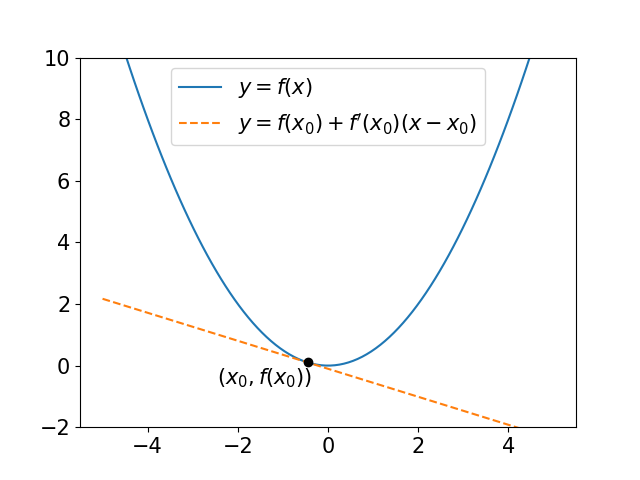
\includegraphics[scale=0.4]{figures/gradient}
    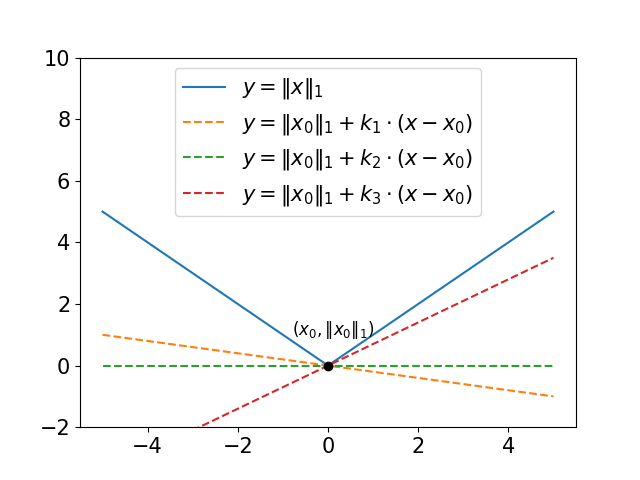
\includegraphics[scale=0.4]{figures/subgradient}
    \caption{Kiri: gradien sebagai kemiringan garis singgung. Kanan: sebuah subgradien sebagai kemiringan garis pendukung.}
\end{figure}

\noindent\textbf{Deskripsi gambar.} Panel kiri memperlihatkan parabola halus dan satu garis singgung putus-putus pada titik yang ditandai. Panel kanan memperlihatkan grafik berbentuk V untuk norma satu dimensi dan tiga garis pendukung dengan kemiringan berbeda yang semuanya melalui titik sudut yang ditandai. Label matematis pada kedua figur dipertahankan persis dari aset sumber.

\Needspace{0.50\textheight}
\begin{example}\
    \begin{enumerate}
        \item Untuk $f(x)=\|x\|_2$, diperoleh
        \[
            \partial f(x)
            = \begin{cases}
                \{\frac{x}{\|x\|_2}\}\quad& x\neq 0,\\
                \overline{B}_{\|\cdot\|_2,1}(0)\quad&\text{selain itu}.
            \end{cases}
        \]
        \item Khususnya, untuk $d=1$ dan $f(x)=|x|$, diperoleh
        \[
            \partial f(x)
            = \begin{cases}
                \{\sign(x)\}\quad& x\neq 0,\\
                [-1,1]\quad&\text{selain itu}.
            \end{cases}
        \]
    \end{enumerate}
\end{example}

% segment-id: d90.hab.v1.ch03.seg0005
\begin{lemma}
    Jika domain $f:X\rightarrow(-\infty,\infty]$ konveks dan subdiferensialnya tak kosong di setiap titik dalam domain, maka $f$ konveks.
\end{lemma}
\begin{proof}
    Misalkan $x,y\in \dom f$, $\lambda\in (0,1)$, dan $g\in \partial f(x+\lambda (y-x))$.
    Menurut definisi subdiferensial,
    \begin{gather}
        f(x+\lambda(y-x)) + \langle g, x - (x+\lambda(y-x))\rangle \leq f(x),\\
        f(x+\lambda(y-x)) + \langle g, y - (x+\lambda(y-x))\rangle \leq f(y),
    \end{gather}
    atau, setara dengan itu,
    \begin{gather}
        f(x+\lambda(y-x)) + \langle g, -\lambda(y-x)\rangle \leq f(x),\\
        f(x+\lambda(y-x)) + \langle g, (1-\lambda)(y - x) \rangle \leq f(y).
    \end{gather}
    Dengan membagi ketaksamaan pertama oleh $\lambda$, membagi yang kedua oleh $1-\lambda$, lalu menjumlahkannya, diperoleh
    \begin{equation}
        \begin{aligned}
            \frac{1}{\lambda} f(x+\lambda(y-x)) + \frac{1}{1-\lambda} f(x+\lambda(y-x))\leq \frac{1}{\lambda} f(x) + \frac{1}{1-\lambda} f(y).
        \end{aligned}
    \end{equation}
    Mengalikan dengan $\lambda (1-\lambda)$ menghasilkan
    \begin{equation}
        \begin{aligned}
            f(x+\lambda(y-x)) \leq (1-\lambda) f(x) + \lambda f(y),
        \end{aligned}
    \end{equation}
    sebagaimana yang diperlukan.
\end{proof}

% segment-id: d90.hab.v1.ch03.seg0006
Seperti disebutkan di atas, subdiferensial dapat kosong. Namun, bagi fungsi konveks berdimensi hingga kita mempunyai jaminan berikut.

Fungsi bernilai real diperluas disebut \emph{sejati (proper)} apabila domain efektifnya tidak kosong dan fungsi itu tidak pernah bernilai minus tak hingga.

\begin{theorem}\label{convexity:thm:nonempty_subgrad}
    Misalkan $X$ ruang bernorma real berdimensi hingga dan $f:X\rightarrow\overline{\R}$ sejati dan konveks. Maka $\partial f(x)\neq \emptyset$ untuk setiap $x\in \dom(f)^\circ$.
\end{theorem}
Sebelum membuktikan hasil ini, kita memerlukan beberapa persiapan.

\begin{lemma}
    Interior suatu himpunan konveks adalah konveks.
\end{lemma}
\begin{proof}
    Misalkan $C$ konveks. Jika $C^\circ=\emptyset$, tidak ada yang perlu dibuktikan; jadi anggap $C^\circ\neq \emptyset$.
    Ambil $x,y\in C^\circ$ dan $\lambda\in (0,1)$. Kita perlu menunjukkan bahwa $x_\lambda\coloneqq\lambda x + (1-\lambda)y\in C^\circ$.
    Terdapat $\epsilon>0$ sedemikian sehingga $B_\epsilon(x),B_\epsilon(y)\subset C^\circ$. Sekarang ambil $z\in B_{\epsilon}(x_\lambda)$. Dengan demikian, $z=x_\lambda + h$ untuk suatu $\|h\|<\epsilon$. Kita dapat menuliskan
    \begin{equation}
        z = \lambda x + (1-\lambda)y + h = \lambda (x+h) + (1-\lambda)(y + h).
    \end{equation}
    Karena $x+h\in B_\epsilon(x)\subset C$ dan $y+h\in B_\epsilon(y)\subset C$, kekonveksan $C$ memberikan $z\in C$. Jadi $B_\epsilon(x_\lambda)\subset C$ dan $x_\lambda\in C^\circ$.
\end{proof}

\begin{lemma}
    Jika $C\subset\R^d,\ d\geq 1$ konveks dan $C^\circ=\emptyset$, maka terdapat hiperbidang $H$ sedemikian sehingga $C\subset H$.
\end{lemma}
\begin{proof}
    Jika \(C\) kosong, sembarang hiperbidang memenuhi kesimpulan. Selanjutnya anggap \(C\) tak kosong. Tanpa mengurangi keumuman, kita boleh menganggap $0\in C$. Jika tidak, pilih sembarang $x_0\in C$ dan tinjau $\widetilde{C}=C-x_0$; pada akhir bukti, hiperbidang yang diperoleh ditranslasikan kembali.

    Kita akan menunjukkan bahwa $C$ merupakan himpunan bagian suatu subruang berdimensi paling besar $d-1$. Andaikan sebaliknya bahwa $C$ memuat $d$ unsur yang bebas linear, yaitu terdapat $x_1,\dots,x_d\in C$ yang bebas linear. Karena $C$ konveks, selubung konveks
    \begin{equation}
        \conv((x_i)_i)=\bigg\{ \sum_{i=1}^d\lambda_i x_i\;\bigg|\; \lambda\in \Delta^d\bigg\}
    \end{equation}
    juga merupakan himpunan bagian $C$. Kita mengklaim bahwa $x_\star\coloneqq\frac{1}{2d}\sum_{i=1}^d x_i\in C^\circ$. Pertama, dari kekonveksan,
    \[
        x_\star=\frac{1}{2d}\sum_{i=1}^d x_i = \sum_{i=1}^d \frac{1}{2d} x_i + \frac{1}{2}0 \in C.
    \]
    Karena $x_i$ bebas linear, setiap $h\in\R^d$ dapat ditulis sebagai $h=\sum_i \lambda_i x_i$. Pemetaan $\lambda\mapsto h$ adalah pemetaan linear bijektif $\R^d\rightarrow\R^d$. Oleh karena itu terdapat $\epsilon>0$ sedemikian sehingga $\|h\|<\epsilon$ mengakibatkan $|\lambda_i|<\frac{1}{2d}$ untuk semua $i$. Khususnya, $\frac{1}{2d}+\lambda_i\in[0,1]$ dan $\sum_{i=1}^d(\frac{1}{2d}+\lambda_i)\in[0,1]$.
    Akibatnya, untuk setiap $\|h\|<\epsilon$,
    \begin{equation}
        x_\star+h = \sum_{i=1}^d \big(\frac{1}{2d} + \lambda_i\big) x_i + \bigg(1 - \sum_i\big(\frac{1}{2d} + \lambda_i\big) \bigg)0\in C.
    \end{equation}
    Jadi, apabila $C$ memuat $d$ unsur bebas linear, interiornya tidak mungkin kosong, sebab $B_\epsilon(x_\star)\subset C$. Ini bertentangan dengan asumsi. Maka $C$ memuat paling banyak $d-1$ unsur bebas linear. Pilih himpunan bebas linear maksimal $x_1,\dots,x_k$ di dalam \(C\); maksimalitas memberikan
    \[
        C\subset \span \{ x_i\mid i=1,\dots,k\}.
    \]
    Dimensi subruang ini kurang dari \(d\), sehingga subruang tersebut termuat dalam suatu hiperbidang. Setelah translasi balik bila diperlukan, diperoleh hiperbidang afin yang memuat himpunan semula.
\end{proof}

% segment-id: d90.hab.v1.ch03.seg0007
Dengan kedua hasil sebelumnya, kita dapat membuktikan teorema hiperbidang pendukung.
\begin{theorem}[Teorema hiperbidang pendukung]
    Misalkan $V$ ruang bernorma real berdimensi hingga, $C\subset V$ tak kosong dan konveks, serta $x_0\in \partial C = \overline{C}\setminus C^\circ$\footnote{yakni batas $C$}. Maka terdapat $a\in V^*$, $a\neq 0$, sedemikian sehingga
    \begin{equation}\label{subgradient:eq:supporting}
        \inner{a}{v}\leq \inner{a}{x_0},\quad v\in C.
    \end{equation}
\end{theorem}
\begin{proof}
    Hasil ini merupakan akibat teorema pemisahan Hahn--Banach. Kita membedakan dua kasus. Pertama, andaikan $C^\circ\neq \emptyset$. Himpunan $C^\circ$ terbuka, konveks, dan tak kosong. Teorema pemisahan Hahn--Banach dapat diterapkan pada $C^\circ$ dan $\{x_0\}$, sehingga ketaksamaan pendukung berlaku pada interior. Karena $C\subset\overline{C^\circ}$ dan fungsional pemisah kontinu, ketaksamaan itu meluas ke seluruh \(C\).

    Sebaliknya, jika $C^\circ$ kosong, lema sebelumnya memberikan hiperbidang afin $H$ yang memuat \(C\). Karena $H$ tertutup dan $x_0\in\overline C$, hiperbidang ini juga memuat titik batas tersebut. Ambil $a\in V^*$ yang tak nol dan $b\in\R$ sedemikian sehingga
    \[
        H=\{x\mid \inner{a}{x} = b\}.
    \]
    Fungsional $a$ ini memenuhi~\eqref{subgradient:eq:supporting}.
\end{proof}

% segment-id: d90.hab.v1.ch03.seg0008
Sekarang kita dapat membuktikan keberadaan subgradien.

\begin{proof}[Bukti \cref{convexity:thm:nonempty_subgrad}]
    Kita ingin menunjukkan bahwa terdapat $g\in X^*$ sedemikian sehingga
    \begin{equation}
        f(x)+\inner{g}{y-x}\leq f(y)
    \end{equation}
    untuk semua $y\in X$. Ini setara dengan
    \begin{equation}\label{subgrad:eq:nonempty_subdiff1}
        \inner{g}{y} - f(y)\leq \inner{g}{x} - f(x).
    \end{equation}
    Bentuk ini menyerupai struktur pemisahan Hahn--Banach. Agar dapat menggunakannya, kita beralih ke epigraf. Perhatikan bahwa $(x,f(x))\in \partial \epi(f)$. Selain itu, kekonveksan $f$ mengakibatkan $\epi(f)$ konveks. Dengan menerapkan teorema hiperbidang pendukung, diperoleh unsur tak nol $(g,-\alpha)\in (X\times\R)^* = X^*\times\R$ sedemikian sehingga\footnote{Tanda minus pada $-\alpha$ dipilih untuk memudahkan perhitungan.}
    \begin{equation}\label{subgrad:eq:nonempty_subdiff2}
        \inner{(g,-\alpha)}{(y,t)}\leq \inner{(g,-\alpha)}{(x,f(x))},\quad (y,t)\in \epi(f).
    \end{equation}
    Ini setara dengan
    \begin{equation}
        \inner{g}{y}-\alpha t \leq \inner{g}{x} - \alpha f(x),\quad (y,t)\in \epi(f).
    \end{equation}
    Kita akan menunjukkan bahwa $\alpha>0$. Andaikan $\alpha<0$. Karena $(x,t)\in \epi(f)$ untuk setiap $t>f(x)$, kita dapat membiarkan $t\rightarrow \infty$ dan memperoleh kontradiksi. Berikutnya, andaikan $\alpha=0$. Maka
    \begin{equation}
        \inner{g}{y-x} \leq 0
    \end{equation}
    bagi semua $y\in\dom(f)$. Karena $x\in \dom(f)^\circ$, hal ini memaksa $g=0$. Padahal teorema pemisahan menghasilkan unsur pemisah yang tak nol; sekali lagi kita memperoleh kontradiksi. Jadi $\alpha>0$, dan kita dapat membagi~\eqref{subgrad:eq:nonempty_subdiff2} dengan $\alpha$ untuk memperoleh
    \begin{equation}
        \inner{\widetilde{g}}{y} - t \leq \inner{\widetilde{g}}{x} - f(x),\quad (y,t)\in \epi(f),
    \end{equation}
    dengan $\widetilde{g} = g/\alpha$. Memilih $t=f(y)$ memberikan $\widetilde{g}\in\partial f(x)$.
\end{proof}

% segment-id: d90.hab.v1.ch03.seg0009
Seperti pada turunan biasa, kita dapat menurunkan beberapa aturan hitung untuk memperoleh subgradien dalam praktik.

\begin{theorem}
    Misalkan $f:V\rightarrow\R$ sejati dan konveks serta $\alpha\geq 0$. Maka, untuk setiap $x\in\dom(f)$,
    \[
        \partial(\alpha f)(x) = \alpha\partial f(x).
    \]
\end{theorem}
\begin{proof}
    Latihan.
\end{proof}

\begin{theorem}
    Misalkan $f,g:V\rightarrow\R$ sejati dan konveks. Untuk setiap $x\in\dom(f)\cap\dom(g)$, berlaku
    \[
        \partial f(x) + \partial g(x)\subset \partial (f+g)(x).
    \]
    Selain itu, jika terdapat $x_0\in \dom(f)^\circ \cap\dom(g)$, maka
    \[
        \partial f(x) + \partial g(x) = \partial (f+g)(x).
    \]
\end{theorem}
\begin{proof}
    Kita hanya membuktikan inklusi pertama. Bukti arah kedua sedikit lebih rumit dan menggunakan teorema pemisahan Hahn--Banach dengan cara yang serupa dengan bukti keberadaan subgradien.

    Ambil $p_1\in \partial f(x)$ dan $p_2\in \partial g(x)$, yaitu
    \begin{equation}
        \begin{aligned}
            f(x) + \langle p_1, y-x\rangle&\leq f(y),\\
            g(x) + \langle p_2, y-x\rangle&\leq g(y).
        \end{aligned}
    \end{equation}
    Menjumlahkan kedua ketaksamaan memberikan
    \begin{equation}
        \begin{aligned}
            f(x)+ g(x) + \langle p_1+p_2, y-x\rangle \leq f(y) + g(y),
        \end{aligned}
    \end{equation}
    sehingga $p_1+p_2\in \partial(f+g)(x)$.
\end{proof}

% segment-id: d90.hab.v1.ch03.seg0010
Terakhir, kita mencatat beberapa \emph{aturan hitung} subdiferensial tanpa bukti.
\begin{theorem}
    Misalkan $f:W\rightarrow\Rb$ sejati, konveks, dan semikontinu bawah, serta $A:V\rightarrow W$ transformasi linear. Definisikan $h(x)=f(Ax+b)$ untuk $b\in W$. Bagi setiap $x\in\dom(h)$ berlaku aturan lemah
    \[
        A^\ast(\partial f(Ax+b))\subseteq\partial h(x).
    \]
    Kesamaan berlaku apabila terdapat $x_0\in V$ dengan $Ax_0+b\in\dom(f)^\circ$.
\end{theorem}

Turunan komposisi fungsi-fungsi terdiferensialkan dihitung dengan aturan rantai. Jadi, turunan $h(x)=g(f(x))$ adalah $D h(x) = Dg(f(x))Df(x)$. Rumus ini dapat diperluas ke kalkulus subdiferensial.
\begin{theorem}
    Misalkan $f:V\rightarrow \R$ konveks, $g:\R\rightarrow \R$ konveks dan tak menurun, serta $h=g\circ f$. Ambil $x\in\dom(f)^\circ$ dan andaikan $g$ terdiferensialkan di $f(x)$. Maka
    \[
        \partial h(x)= g'(f(x))\partial f(x).
    \]
\end{theorem}

% segment-id: d90.hab.v1.ch03.seg0011
\begin{theorem}
    Misalkan $f:V\to(-\infty, \infty]$ fungsi konveks sejati. Maka
    \[
        x^\ast\in\arg\min_{x\in V} f(x)
    \]
    jika dan hanya jika $0\in\partial f(x^\ast)$.
\end{theorem}
\begin{proof}
    Pernyataan ini langsung mengikuti ketaksamaan subgradien
    \[
        f(x)\geq f(x^\ast)+\inner{0}{x-x^\ast}
    \]
    bagi setiap $x\in\dom f$.
\end{proof}

\begin{theorem}
    Misalkan $f:V\rightarrow(-\infty,\infty]$ sejati dan konveks, serta $C\subseteq V$ konveks dengan $\dom(f)^\circ\cap C^\circ \neq\emptyset$. Titik $x^\ast\in C$ merupakan solusi persoalan optimisasi berkendala jika dan hanya jika terdapat $g\in \partial f(x^\ast)$ sedemikian sehingga
    \[
        \inner{g}{x-x^\ast}\geq 0
    \]
    bagi semua $x\in C$.
\end{theorem}

\chapter{Penurunan subgradien terproyeksi}

% segment-id: d90.hab.v1.ch04.seg0001
Misalkan \(V\) ruang Hilbert real, \(C\subset V\) himpunan tak kosong, tertutup, dan konveks, serta \(f:V\rightarrow\R\) fungsi konveks. Kita tertarik menyelesaikan masalah
\begin{equation}
    \min_{x\in C} f(x).
\end{equation}
Kita mengasumsikan bahwa himpunan peminim tidak kosong dan menetapkan
\(x^*\in\arg\min_{x\in C}f(x)\). Masalah berkendala di atas selalu dapat ditulis sebagai masalah tak berkendala melalui
\begin{equation}
    \min_{x\in V} f(x) + \delta_C(x),
\end{equation}
dengan \(\delta_C\) fungsi indikator himpunan \(C\).\footnote{Formulasi ini memakai \(f\) yang terdefinisi pada seluruh \(V\), termasuk di luar \(C\).}

Ingat kembali metode optimisasi numerik paling dasar untuk masalah semacam ini ketika \(C=V\) dan \(f\) terdiferensialkan: penurunan gradien (atau penurunan \emph{tercuram}). Kita memilih nilai awal \(x_0\), lalu untuk \(k=0,1,\dots\) melakukan pembaruan
\begin{equation}
    x_{k+1} = x_k-\tau_k \nabla f(x_k),
\end{equation}
dengan \(\tau_k>0\) menyatakan ukuran langkah. Algoritma \emph{baru} pertama yang kita tinjau ialah versi subgradien dari penurunan tercuram: untuk \(k=0,1,\dots\),
\begin{equation}
    \begin{cases}
        g_k &\in \partial f(x_k),\\
        x_{k+1} &= x_k-\tau_k g_k.
    \end{cases}
\end{equation}
Jika \(C\neq V\), masalah segera dapat muncul: mungkin saja \(x_{k+1}\notin C\). Dalam hal itu, iterasi yang memakai subdiferensial \(f+\delta_C\) tidak lagi terdefinisi karena \(\partial\delta_C(x)=\emptyset\) untuk \(x\notin C\). Karena itu, kita perlu memastikan setiap iterasi baru tetap berada di \(C\); untuk tujuan ini kita memakai \emph{proyeksi}.

% segment-id: d90.hab.v1.ch04.seg0002
\begin{theorem}[Teorema proyeksi]
    Misalkan \(V\) ruang Hilbert real dan \(C\subset V\) tak kosong, tertutup, dan konveks. Fungsi berikut terdefinisi dengan baik:
    \begin{equation}
        \begin{aligned}
            \proj_C:V&\rightarrow C,\\
            x&\mapsto\arg\min_{y\in C}\|x-y\|.
        \end{aligned}
    \end{equation}
\end{theorem}
\begin{proof}
    Kita perlu menunjukkan bahwa minimum tercapai secara tunggal. Tetapkan
    \(d=\inf_{y\in C}\|y-x\|\), dan ambil barisan peminimum \((y_n)_n\subset C\), yaitu
    \begin{equation}
        \lim_n \|y_n-x\| = d.
    \end{equation}
    Karena \(C\) konveks, \((y_n+y_m)/2\in C\). Identitas jajaran genjang memberi
    \[
        \|y_n-y_m\|^2
        =2\|y_n-x\|^2+2\|y_m-x\|^2
        -4\left\|\frac{y_n+y_m}{2}-x\right\|^2
        \leq 2\|y_n-x\|^2+2\|y_m-x\|^2-4d^2.
    \]
    Ruas kanan menuju nol ketika \(m,n\rightarrow\infty\), sehingga \((y_n)_n\) merupakan barisan Cauchy. Kelengkapan \(V\) menghasilkan \(y_n\rightarrow\widehat y\in V\), sedangkan ketertutupan \(C\) menghasilkan \(\widehat y\in C\). Dari kontinuitas norma diperoleh
    \begin{equation}
        \|\widehat y-x\| = \lim_n \|y_n-x\| = d,
    \end{equation}
    jadi peminim memang ada.

    Untuk ketunggalan, andaikan \(y_1\neq y_2\) keduanya peminim. Identitas jajaran genjang memberikan
    \begin{equation}
        \begin{aligned}
            \left\|\frac{y_1+y_2}{2}-x\right\|^2
            &=\frac{1}{2}\|y_1-x\|^2+\frac{1}{2}\|y_2-x\|^2
              -\frac{1}{4}\|y_1-y_2\|^2\\
            &<d^2.
        \end{aligned}
    \end{equation}
    Namun \((y_1+y_2)/2\in C\), yang bertentangan dengan definisi \(d\). Jadi peminimnya tunggal.
\end{proof}

% segment-id: d90.hab.v1.ch04.seg0003
Dengan proyeksi, kita memperoleh cara mengatasi masalah \emph{keluar} dari \(C\): metode subgradien terproyeksi. Pilih \(x_0\in C\); kemudian, untuk \(k=0,1,\dots\) dan \(\tau_k\geq0\), tetapkan
\begin{equation}\label{subgradient:eq:projectedSG}
    \begin{cases}
        g_k &\in \partial f(x_k),\\
        x_{k+1} &= \proj_C( x_k-\tau_k g_k) .
    \end{cases}
\end{equation}
Untuk membuktikan konvergensi metode ini, kita memerlukan beberapa hasil bantu.

\begin{lemma}
    Misalkan \(V\) ruang Hilbert real dan \(C\subset V\) tak kosong, tertutup, dan konveks. Maka
    \begin{equation}
        \inner{x-\proj_C(x)}{y-\proj_C(x)}\leq 0,\quad y\in C.
    \end{equation}
    Khususnya, jika \(C\) subruang,\footnote{Artinya, \(C\) memenuhi definisi ruang vektor.} maka
    \begin{equation}
        \inner{x-\proj_C(x)}{y}= 0,\quad y\in C.
    \end{equation}
\end{lemma}
\begin{proof}
    Untuk setiap \(y\in C\), kita mempunyai
    \begin{equation}
        \begin{aligned}
            \|\proj_C(x)-x\|^2
            &\leq \|y-x\|^2\\
            &= \|y - \proj_C(x) + \proj_C(x)-x\|^2\\
            &= \|y-\proj_C(x)\|^2
              + 2 \inner{y-\proj_C(x)}{\proj_C(x)-x}
              + \|\proj_C(x)-x\|^2.
        \end{aligned}
    \end{equation}
    Akibatnya,
    \begin{equation}
        \begin{aligned}
            0\leq \|y-\proj_C(x)\|^2
            + 2 \inner{y-\proj_C(x)}{\proj_C(x)-x}.
        \end{aligned}
    \end{equation}
    Ambil sebarang \(z\in C\), lalu pada ketaksamaan di atas masukkan
    \(y=\proj_C(x) + t(z-\proj_C(x))\) untuk \(t\in (0,1)\). Kita memperoleh
    \begin{equation}
        \begin{aligned}
            0\leq t^2 \|z-\proj_C(x)\|^2
            + 2 t\inner{z-\proj_C(x)}{\proj_C(x)-x}.
        \end{aligned}
    \end{equation}
    Setelah dibagi dengan \(t>0\),
    \begin{equation}
        \begin{aligned}
            0\leq t \|z-\proj_C(x)\|^2
            + 2 \inner{z-\proj_C(x)}{\proj_C(x)-x}.
        \end{aligned}
    \end{equation}
    Dengan mengambil limit \(t\rightarrow 0\), kita memperoleh hasil yang diinginkan. Kesamaan untuk kasus subruang ditinggalkan sebagai latihan.
\end{proof}

% segment-id: d90.hab.v1.ch04.seg0004
\begin{prop}
    Misalkan \(V\) ruang Hilbert real dan \(C\subset V\) tak kosong, tertutup, dan konveks. Proyeksi pada \(C\) bersifat tak ekspansif, yaitu kontinu Lipschitz dengan konstanta satu:
    \begin{equation}
        \|\proj_C(x_1)-\proj_C(x_2)\|\leq \|x_1-x_2\|.
    \end{equation}
\end{prop}
\begin{proof}
    Tanpa mengurangi keumuman, andaikan
    \(\|\proj_C(x_2)-\proj_C(x_1)\|^2 \neq 0\), sebab jika tidak, tidak ada yang perlu dibuktikan. Kita memperoleh
    \begin{equation}
        \begin{aligned}
            \|\proj_C(x_2)-\proj_C(x_1)\|^2
            &= \inner{\proj_C(x_2)-\proj_C(x_1)}{\proj_C(x_2)-x_1+x_1-\proj_C(x_1)}\\
            &= \inner{\proj_C(x_2)-\proj_C(x_1)}{\proj_C(x_2)-x_1}\\
            &\quad+ \inner{\proj_C(x_2)-\proj_C(x_1)}{x_1-\proj_C(x_1)}\\
            &\leq \inner{\proj_C(x_2)-\proj_C(x_1)}{\proj_C(x_2)-x_1}\\
            &= \inner{\proj_C(x_2)-\proj_C(x_1)}{\proj_C(x_2)-x_2+x_2-x_1}\\
            &\leq \inner{\proj_C(x_1)-\proj_C(x_2)}{x_2-\proj_C(x_2)}\\
            &\quad+ \inner{\proj_C(x_2)-\proj_C(x_1)}{x_2-x_1}\\
            &\leq \inner{\proj_C(x_2)-\proj_C(x_1)}{x_2-x_1}\\
            &\leq \|\proj_C(x_2)-\proj_C(x_1)\|\|x_2-x_1\|.
        \end{aligned}
    \end{equation}
    Membagi dengan \(\|\proj_C(x_2)-\proj_C(x_1)\|\neq 0\) menghasilkan kesimpulan.
\end{proof}

% segment-id: d90.hab.v1.ch04.seg0005
\begin{lemma}[Ketaksamaan fundamental metode subgradien terproyeksi]\label{lemma:subgradient:fundamental}
    Misalkan \(x^*\in\arg\min_{x\in C}f(x)\), dan misalkan \(x_k\) adalah iterasi metode subgradien terproyeksi~\eqref{subgradient:eq:projectedSG}, dengan \(g_k\in\partial f(x_k)\) dan \(\tau_k\geq0\). Maka
    \begin{equation}
        \|x_{k+1}-x^*\|^2
        \leq \|x_k- x^*\|^2 - 2\tau_k (f(x_k)-f(x^*)) + \tau_k^2\|g_k\|^2.
    \end{equation}
\end{lemma}
\begin{proof}
    Dari definisi subgradien,
    \(f(x_k)+ \inner{g_k}{x^*-x_k}\leq f(x^*)\). Karena \(x^*\in C\), kita mempunyai \(\proj_C(x^*)=x^*\). Ketakspansifan proyeksi lalu memberikan
    \begin{equation}\label{eq:subgradient:fundamental}
        \begin{aligned}
            \|x_{k+1}-x^*\|^2
            &= \|\proj_C(x_k-\tau_kg_k) - \proj_C(x^*)\|^2\\
            &\leq \|x_k-\tau_k g_k - x^*\|^2\\
            &= \|x_k- x^*\|^2 - 2\tau_k \inner{g_k}{x_k-x^*} + \tau_k^2\|g_k\|^2\\
            &\leq \|x_k- x^*\|^2 - 2\tau_k (f(x_k)-f(x^*)) + \tau_k^2\|g_k\|^2.
        \end{aligned}
    \end{equation}
\end{proof}

% segment-id: d90.hab.v1.ch04.seg0006
Hal yang wajar dilakukan sekarang ialah memakai hasil sebelumnya untuk menentukan ukuran langkah optimal. Lebih tepatnya, dengan meminimumkan ruas kanan~\eqref{eq:subgradient:fundamental} terhadap \(\tau_k\), kita memperoleh
\begin{equation}
    \tau_k = \frac{f(x_k)-f(x^*)}{\|g_k\|^2}
\end{equation}
jika \(g_k\neq 0\), dan kita menetapkan \(\tau_k=0\) jika \(g_k=0\). Ukuran langkah ini disebut aturan ukuran langkah Polyak.

Sebagai latihan, buktikan bahwa jika fungsi konveks \(f:V\rightarrow\R\) bersifat \(L\)-Lipschitz secara global pada \(V\), maka setiap \(g\in\partial f(x)\) memenuhi \(\|g\|\leq L\). Pada hasil-hasil berikut, kita memakai langsung batas pada subgradien yang dipilih, sehingga juga mencakup situasi berkendala yang tidak memenuhi asumsi Lipschitz global tersebut.

\begin{theorem}
    Andaikan subgradien yang dipilih pada iterasi memenuhi \(\|g_k\|\leq L\). Dengan aturan ukuran langkah Polyak
    \begin{equation}
        \tau_k = \frac{f(x_k)-f(x^*)}{\|g_k\|^2}\quad\text{jika }g_k\neq0,
        \qquad \tau_k=0\quad\text{jika }g_k=0.
    \end{equation}
    metode subgradien terproyeksi~\eqref{subgradient:eq:projectedSG} memenuhi
    \begin{enumerate}
        \item \(\|x_{k+1}-x^*\|^2\leq \|x_k-x^*\|^2\), dengan ketaksamaan ketat jika \(f(x_k)>f(x^*)\);
        \item \(f(x_k)\rightarrow f(x^*)\) ketika \(k\rightarrow\infty\); dan
        \item \(f_{\mathrm{best}}^N-f(x^*)\leq \dfrac{L\|x_1-x^*\|}{\sqrt{N}}\), dengan \(f_{\mathrm{best}}^N = \min_{k=1,\dots,N}f(x_k)\).
    \end{enumerate}
\end{theorem}
\begin{proof}
    Tanpa mengurangi keumuman, kita boleh mengasumsikan \(f(x^*)=0\). Jika tidak, cukup tinjau \(\widetilde f(x)\coloneq f(x)-f(x^*)\). Dari~\cref{lemma:subgradient:fundamental} dan aturan ukuran langkah diperoleh
    \begin{equation}
        \begin{aligned}
            \|x_{k+1}-x^*\|^2
            &\leq \|x_k - x^*\|^2 - 2\tau_k f(x_k) +\tau_k^2\|g_k\|^2\\
            &= \|x_k - x^*\|^2 - a_k,
        \end{aligned}
    \end{equation}
    dengan \(a_k=f(x_k)^2/\|g_k\|^2\) jika \(g_k\neq0\), dan nol jika \(g_k=0\). Jika \(g_k=0\), kekonveksan memberi \(f(x_k)=f(x^*)\). Karena itu, pengurangan bersifat ketat tepat ketika celah nilai fungsi positif.

    Dengan menata ulang dan menjumlahkan untuk \(k=1,\dots,N\), kita memperoleh
    \begin{equation}
        \sum_{k=1}^{N} a_k
        \leq \|x_1-x^*\|^2 - \|x_{N+1}-x^*\|^2
        \leq \|x_1-x^*\|^2.
    \end{equation}
    Karena \(\|g_k\|\leq L\),
    \begin{equation}
        \sum_{k=1}^{N} f(x_k)^2
        \leq \sum_{k=1}^{N} L^2 a_k
        \leq L^2 \|x_1-x^*\|^2.
    \end{equation}
    Batas ini berlaku untuk setiap \(N\), sehingga \(f(x_k)\rightarrow0\). Selain itu,
    \begin{equation}
        N (f_{\mathrm{best}}^N)^2
        \leq \sum_{k=1}^{N} f(x_k)^2
        \leq L^2\|x_1-x^*\|^2,
    \end{equation}
    yaitu
    \begin{equation}
        f_{\mathrm{best}}^N\leq \frac{L\|x_1-x^*\|}{\sqrt{N}}.
    \end{equation}
\end{proof}

% segment-id: d90.hab.v1.ch04.seg0007
\begin{cor}
    Untuk mencapai ketelitian \(f_{\mathrm{best}}^N - f(x^*)\leq \epsilon\), kita memerlukan
    \[
        N=\Oc\!\left(\frac{L^2\|x_1-x^*\|^2}{\epsilon^2}\right)
    \]
    iterasi.
\end{cor}

\begin{rem}
    Ingat bahwa metode gradien mulus standar mencapai kompleksitas \(\Oc(1/\epsilon)\).
\end{rem}

Walaupun hasil konvergensi dengan aturan ukuran langkah Polyak menarik secara teoretis dan memberi batas kasus terburuk untuk iterasi terbaik, dalam praktiknya ukuran langkah tersebut tidak dapat dihitung tanpa mengetahui \(f(x^*)\). Berikut ini kita berikan hasil konvergensi yang lebih umum.

\begin{theorem}
    Andaikan subgradien yang dipilih memenuhi \(\|g_k\|\leq L\), dan ukuran langkah \(\tau_k>0\) memenuhi
    \[
        \frac{\sum_{k=1}^n\tau_k}{\sum_{k=1}^n\tau_k^2}\rightarrow \infty
        \qquad\text{ketika }n\rightarrow\infty.
    \]
    Maka
    \[
        f^n_{\mathrm{best}}-f(x^*)
        \leq
        \frac{\|x_1-x^*\|^2+L^2\sum_{k=1}^n\tau_k^2}
             {2\sum_{k=1}^n\tau_k}
        \longrightarrow0.
    \]
\end{theorem}
\begin{proof}
    Sekali lagi, untuk menyederhanakan notasi, andaikan \(f(x^*)=0\). Dengan memakai \(\|g_k\|\leq L\) dan menjumlahkan ketaksamaan fundamental~\cref{lemma:subgradient:fundamental} untuk \(k=1,\dots,n\), kita memperoleh
    \begin{equation}
        2\sum_{k=1}^n\tau_k f(x_k)
        \leq \|x_1-x^*\|^2 + L^2 \sum_{k=1}^n \tau_k^2.
    \end{equation}
    Tuliskan
    \[
        \sigma_n = \frac{\sum_{k=1}^n\tau_k}{\sum_{k=1}^n\tau_k^2}.
    \]
    Karena \(f^n_{\mathrm{best}}\leq f(x_k)\),
    \begin{equation}
        f^n_{\mathrm{best}}
        \leq \frac{\sum_{k=1}^n\tau_kf(x_k)}{\sum_{k=1}^n\tau_k}
        \leq \frac{\|x_1-x^*\|^2}{2\sum_{k=1}^n\tau_k}
        +\frac{L^2}{2\sigma_n}.
    \end{equation}
    Hipotesis \(\sigma_n\rightarrow\infty\) juga memaksa \(\sum_{k=1}^n\tau_k\rightarrow\infty\); karena itu, kedua suku pada ruas kanan menuju nol.
\end{proof}

% segment-id: d90.hab.v1.ch04.seg0008
Varian hasil konvergensi juga dapat diperoleh, misalnya jika \(C\) kompak; lihat~\cite{beck2017first} untuk perinciannya.

Konvergensi dapat dipercepat dan juga \emph{ditransfer} dari nilai fungsi ke iterasi \((x_k)_k\) jika kita menambahkan asumsi bahwa \(f\) konveks kuat.

\begin{theorem}
    Andaikan \(f\) konveks kuat dengan parameter \(\mu>0\) pada \(C\), dan subgradien yang dipilih memenuhi \(\|g_k\|\leq L\).\footnote{Batas ini dikenakan pada subgradien yang benar-benar dipilih oleh algoritma; batas tersebut tidak disimpulkan hanya dari sifat Lipschitz relatif pada \(C\).} Mulai dari \(x_1\in C\), gunakan ukuran langkah
    \(\tau_k = \dfrac{2}{\mu k}\) untuk \(k\geq1\). Untuk \(n\geq2\), metode subgradien terproyeksi~\eqref{subgradient:eq:projectedSG} memenuhi
    \begin{enumerate}
        \item \(f^n_{\mathrm{best}}-f(x^*)\leq \dfrac{2L^2}{\mu (n-1)}\); dan
        \item \(\|x_n-x^*\|\leq \dfrac{2L}{\mu \sqrt{n-1}}\).
    \end{enumerate}
\end{theorem}
\begin{proof}
    Seperti sebelumnya, tanpa mengurangi keumuman, tetapkan \(f(x^*)=0\). Kekonveksan kuat memperbaiki ketaksamaan fundamental menjadi
    \begin{equation}
        \begin{aligned}
            \|x_{k+1}-x^*\|^2
            &\leq (1-\mu\tau_k)\|x_k- x^*\|^2 - 2\tau_k f(x_k) + \tau_k^2\|g_k\|^2\\
            &\leq (1-\mu\tau_k)\|x_k- x^*\|^2 - 2\tau_k f(x_k) + \tau_k^2L^2.
        \end{aligned}
    \end{equation}
    Dengan menata ulang dan membagi dengan \(2\tau_k\), diperoleh
    \begin{equation}
        \begin{aligned}
            f(x_k)
            \leq -\frac{\tau_k^{-1}}{2}\|x_{k+1}-x^*\|^2
            + \frac{\tau_k^{-1}-\mu}{2}\|x_k- x^*\|^2
            + \frac{\tau_k}{2}L^2.
        \end{aligned}
    \end{equation}
    Memasukkan \(\tau_k = 2/(\mu k)\) menghasilkan
    \begin{equation}
        \begin{aligned}
            f(x_k)
            \leq -\frac{\mu k}{4} \|x_{k+1}-x^*\|^2
            + \frac{\mu(k-2)}{4}\|x_k- x^*\|^2
            + \frac{1}{\mu k}L^2.
        \end{aligned}
    \end{equation}
    Kalikan dengan \(k-1\), lalu jumlahkan terhadap \(k=1,\dots,n\). Suku jarak meneleskop, sehingga
    \begin{equation}
        \sum_{k=1}^{n} (k-1)f(x_k)
        \leq -\frac{\mu n(n-1)}{4} \|x_{n+1}-x^*\|^2
        + \frac{1}{\mu}\sum_{k=1}^{n}\frac{k-1}{k}L^2.
    \end{equation}
    Karena \(\sum_{k=1}^{n} (k-1)=n(n-1)/2\) dan
    \(\sum_{k=1}^{n}(k-1)/k\leq n\), kita memperoleh
    \begin{equation}\label{subgradient:eq:strongly}
        \frac{n(n-1)}{2} f^n_{\mathrm{best}}
        \leq \sum_{k=1}^{n} (k-1)f(x_k)
        \leq -\frac{\mu n(n-1)}{4} \|x_{n+1}-x^*\|^2
        + \frac{nL^2}{\mu}.
    \end{equation}
    Dengan membuang suku jarak yang tak positif, diperoleh
    \begin{equation}
        f^n_{\mathrm{best}} \leq \frac{2L^2}{\mu(n-1)}.
    \end{equation}

    Untuk batas iterasi, buang suku \(-2\tau_k f(x_k)\leq0\) dari ketaksamaan fundamental yang diperbaiki. Dengan \(d_k=\|x_k-x^*\|\),
    \begin{equation}
        d_{k+1}^2\leq\left(1-\frac{2}{k}\right)d_k^2
        +\frac{4L^2}{\mu^2k^2}.
    \end{equation}
    Untuk \(k=1\), ketaksamaan ini memberi \(d_2^2\leq4L^2/\mu^2\). Jika
    \(d_k^2\leq4L^2/[\mu^2(k-1)]\), substitusi pada relasi di atas memberikan
    \[
        d_{k+1}^2
        \leq \frac{4L^2}{\mu^2}
        \left(\frac{k-2}{k(k-1)}+\frac{1}{k^2}\right)
        \leq \frac{4L^2}{\mu^2k}.
    \]
    Induksi membuktikan \(\|x_n-x^*\|\leq2L/[\mu\sqrt{n-1}]\) untuk setiap \(n\geq2\).
\end{proof}

\chapter{Metode gradien proksimal}

% segment-id: d90.hab.v1.ch05.seg0001
Kita telah melihat dalam bukti (dan latihan praktis) bahwa metode subgradien tidak memberikan konvergensi yang ideal. Dalam kasus dasar atau terburuk, nilai fungsi berkonvergensi dengan orde \(\Oc(1/\sqrt{k})\), dan konvergensi memerlukan ukuran langkah yang mengecil. Dalam bab ini, kita akan memperkenalkan alternatif bagi subgradien (eksplisit) dalam optimisasi.

Perhatikan masalah tak berkendala
\begin{equation}\label{proximal:eq:problem}
    \min_x f(x),
\end{equation}
dengan \(f:\R^d\rightarrow(-\infty,\infty]\) proper, semikontinu bawah, dan konveks. Ingat pembaruan metode subgradien \(x_{k+1}=x_k-\tau_k g_k\), \(g_k\in\partial f(x_k)\), atau, secara ekuivalen, \(x_{k+1}\in x_k-\tau_k\partial f(x_k)\). Untuk \(\tau_k>0\), kita usulkan pembaruan implisit
\begin{equation}\label{proximal:eq:intro}
    x_{k+1}\in x_k-\tau_k\partial f(x_{k+1}).
\end{equation}
Pada tahap ini belum jelas apakah metode tersebut terdefinisi dengan baik. Namun, jika memang terdefinisi, secara intuitif kestabilannya dapat membaik karena arah pembaruan dipilih dengan \emph{melihat ke masa depan}. Gagasan ini selaras dengan kestabilan metode implisit untuk mendiskretkan persamaan diferensial (\cf~\emph{Euler implisit}).

Jika kita amati~\eqref{proximal:eq:intro} lebih dekat, aturan itu dapat ditulis sebagai
\begin{equation}
    0\in\partial\biggl(\frac{1}{2}\|\cdot-x_k\|^2+\tau_k f\biggr)(x_{k+1}),
\end{equation}
yang merupakan kondisi optimalitas untuk
\begin{equation}
    \min_x\frac{1}{2}\|x-x_k\|^2+\tau_k f(x).
\end{equation}
Hal ini membawa kita pada definisi berikut.
\begin{defn}[Operator proksimal]
    Operator atau pemetaan proksimal dari \(f:\R^d\rightarrow(-\infty,\infty]\) didefinisikan sebagai pemetaan
    \begin{equation}
        \begin{aligned}
            \prox_f:\R^d&\rightarrow 2^{\R^d},\\
            x&\mapsto\arg\min_{y\in\R^d}\frac{1}{2}\|y-x\|^2+f(y).
        \end{aligned}
    \end{equation}
\end{defn}

Kita biasanya menyebut \(\prox_f\) sebagai \enquote{proks}. Sebagai pemetaan bernilai himpunan, proks selalu dapat dituliskan; tetapi pemetaan itu baru berguna ketika \(\prox_f(x)\neq\emptyset\). Kita dapat membuktikan hasil berikut.

% segment-id: d90.hab.v1.ch05.seg0002
\begin{lemma}
    Misalkan \(f:\R^d\rightarrow(-\infty,\infty]\) proper, konveks, dan semikontinu bawah. Pemetaan proksimal bernilai tunggal. Lebih lanjut, \(y=\prox_f(x)\) jika dan hanya jika \(0\in(y-x)+\partial f(y)\).
\end{lemma}
\begin{rem}
    Berdasarkan karakterisasi \(0\in(y-x)+\partial f(y)\), kita sering menulis proks sebagai \(\prox_f(x)=(\Id+\partial f)^{-1}(x)\).
\end{rem}
\begin{proof}
    Demi kesederhanaan, andaikan \(\dom(f)^\circ\neq\emptyset\); untuk kasus umum, lihat~\cite{beck2017first}.

    Ambil \(g\in\partial f(y_0)\) untuk suatu \(y_0\in\dom(f)^\circ\). Kita mempunyai
    \begin{equation}
        f(y_0)+\inner{g}{y-y_0}+\frac{1}{2}\|x-y\|^2
        \leq f(y)+\frac{1}{2}\|x-y\|^2.
    \end{equation}
    Oleh karena itu (mengapa?), pemetaan \(y\mapsto f(y)+\frac{1}{2}\|x-y\|^2\) bersifat koersif. Pemetaan ini juga mewarisi sifat semikontinu bawah dan proper dari \(f\). Dengan metode langsung untuk fungsi proper, semikontinu bawah, dan koersif di ruang berdimensi hingga, terdapat solusi bagi
    \begin{equation}\label{proximal:eq:prox_proof}
        \min_{y\in\R^d}\frac{1}{2}\|y-x\|^2+f(y).
    \end{equation}
    Untuk keunikan, definisikan \(q_x(y)=\frac{1}{2}\|y-x\|^2+f(y)\) dan andaikan \(y_1\neq y_2\) adalah dua peminim. Karena suku kuadrat konveks ketat dan \(f\) konveks, untuk \(\bar y=(y_1+y_2)/2\) berlaku
    \begin{equation}
        \begin{aligned}
            q_x(\bar y)
            <&\frac{1}{2}\bigl(q_x(y_1)+q_x(y_2)\bigr)\\
            =&\min_{y\in\R^d}q_x(y),
        \end{aligned}
    \end{equation}
    sebuah kontradiksi. Pernyataan terakhir merupakan kondisi optimalitas bagi~\eqref{proximal:eq:prox_proof}.
\end{proof}

% segment-id: d90.hab.v1.ch05.seg0003
Setelah mengetahui bahwa proks terdefinisi dengan baik, kita dapat mendefinisikan metode gradien proksimal. Secara khusus, perhatikan masalah
\begin{equation}\label{proximal:eq:composite}
    \min_{x\in\R^d}F(x)\coloneqq f(x)+g(x),
\end{equation}
dengan \(f\) konveks dan \(L\)-halus, yakni terdiferensialkan dengan gradien \(L\)-Lipschitz, sedangkan \(g\) proper, konveks, dan semikontinu bawah. Masalah semacam ini sering muncul dalam praktik dan mencakup masalah semula dengan mengambil \(f\equiv0\). Untuk \(k=0,1,\dots\), metode gradien proksimal didefinisikan oleh
\begin{equation}\label{proximal:eq:prox_grad}
    \begin{aligned}
        x_{k+1}=\prox_{\tau_k g}\bigl(x_k-\tau_k\nabla f(x_k)\bigr).
    \end{aligned}
\end{equation}
Jadi, kita melakukan langkah gradien atau eksplisit terhadap \(f\), lalu langkah proksimal atau implisit terhadap \(g\).

Sebagai hasil sederhana pertama, kita menunjukkan bahwa titik tetap metode gradien proksimal tepat sama dengan titik optimal.
\begin{lemma}
    Untuk suatu \(\tau>0\) yang tetap dan \(x\in\R^d\), pernyataan berikut ekuivalen:
    \begin{equation}
        x=\prox_{\tau g}\bigl(x-\tau\nabla f(x)\bigr)
        \quad\Longleftrightarrow\quad
        0\in\partial(f+g)(x).
    \end{equation}
    Dengan demikian, \(x\) adalah titik tetap jika dan hanya jika \(x\) menyelesaikan~\eqref{proximal:eq:composite}.
\end{lemma}
\begin{proof}
    Karakterisasi optimalitas proks memberikan ekuivalensi
    \begin{equation}
        x=\prox_{\tau g}\bigl(x-\tau\nabla f(x)\bigr)
        \quad\Longleftrightarrow\quad
        0\in\tau\nabla f(x)+\tau\partial g(x).
    \end{equation}
    Karena \(\tau>0\), serta menurut aturan jumlah dan aturan skala untuk subdiferensial,
    \begin{equation}
        0\in\tau\bigl(\nabla f(x)+\partial g(x)\bigr)
        \quad\Longleftrightarrow\quad
        0\in\partial(f+g)(x).
    \end{equation}
    Untuk fungsi konveks \(F=f+g\), kondisi terakhir ekuivalen dengan optimalitas \(x\).
\end{proof}

% segment-id: d90.hab.v1.ch05.seg0004
Selain proks, kita mendefinisikan selubung Moreau sebagai nilai infimum dari objektif yang digunakan untuk proks.
\begin{defn}[Selubung Moreau]
    Misalkan \(f:\R^d\rightarrow(-\infty,\infty]\) dan \(\tau>0\). Selubung Moreau \(M_f^\tau:\R^d\rightarrow[-\infty,\infty]\) didefinisikan oleh
    \begin{equation}
        M_f^\tau(x)\coloneqq\inf_{y\in\R^d}\frac{1}{2\tau}\|x-y\|^2+f(y).
    \end{equation}
\end{defn}

\begin{lemma}
    Misalkan \(f:\R^d\rightarrow(-\infty,\infty]\) proper, konveks, dan semikontinu bawah, serta \(\tau>0\). Selubung Moreau selalu bernilai real (yakni berhingga), dan
    \begin{equation}
        M_f^\tau(x)
        =\frac{1}{2\tau}\bigl\|x-\prox_{\tau f}(x)\bigr\|^2
        +f\bigl(\prox_{\tau f}(x)\bigr).
    \end{equation}
\end{lemma}
\begin{proof}
    Latihan. Terapkan lemma keberadaan dan keunikan proks pada \(\tau f\), lalu substitusikan peminim unik tersebut ke dalam definisi infimum.
\end{proof}

\begin{example}
    Kita tinjau beberapa contoh pemetaan proksimal dan selubung Moreau yang sering muncul:
    \begin{enumerate}
        \item Misalkan \(C\subset\R^d\) tak kosong, tertutup, dan konveks, dan perhatikan fungsi indikator \(\delta_C\). Maka
        \begin{equation}
            \prox_{\tau\delta_C}(x)=\proj_C(x),
            \qquad
            M_{\delta_C}^{\tau}(x)=\frac{1}{2\tau}\operatorname{dist}(x,C)^2.
        \end{equation}
        \item Secara khusus, jika \(C=\{x\in\R^d\mid\|x\|_\infty\leq1\}\), maka
        \begin{equation}
            \bigl(\prox_{\tau\delta_C}(x)\bigr)_i
            =\frac{x_i}{\max\{1,|x_i|\}}.
        \end{equation}
        \item Jika \(f(x)=\|x\|_1\), pemetaan proksimalnya adalah operator \emph{ambang lunak}
        \begin{equation}
            \bigl(\prox_{\tau f}(x)\bigr)_i=
            \begin{cases}
                x_i-\tau & x_i>\tau,\\
                x_i+\tau & x_i<-\tau,\\
                0 & x_i\in[-\tau,\tau].
            \end{cases}
        \end{equation}
        Untuk \(d=1\), selubung Moreau-nya tepat merupakan fungsi Huber
        \begin{equation}
            M_{|\cdot|}^{\tau}(x)=
            \begin{cases}
                \dfrac{|x|^2}{2\tau} & |x|\leq\tau,\\
                |x|-\dfrac{\tau}{2} & |x|>\tau.
            \end{cases}
        \end{equation}
    \end{enumerate}
\end{example}

% segment-id: d90.hab.v1.ch05.seg0005
\begin{lemma}[Aturan komputasi untuk proks]
    Misalkan semua fungsi dasar yang muncul di bawah proper, semikontinu bawah, dan konveks pada domain berdimensi hingga yang dinyatakan. Aturan berikut berlaku:
    \begin{enumerate}
        \item Jika \(x=(x_1,\dots,x_m)\in\R^{d_1}\times\cdots\times\R^{d_m}\cong\R^d\), \(x_i\in\R^{d_i}\), \(\sum_i d_i=d\), dan \(f(x)=\sum_i f_i(x_i)\), maka \(\prox_f(x)=\bigl(\prox_{f_i}(x_i)\bigr)_i\).
        \item Jika \(f(x)=\alpha g(x)+b\) dengan \(\alpha>0\) dan \(b\in\R\), maka \(\prox_f=\prox_{\alpha g}\).
        \item Jika \(f(x)=g(\alpha x+b)\) dengan \(\alpha\neq0\) dan \(b\in\R^d\), maka \(\prox_f(x)=\alpha^{-1}\bigl(\prox_{\alpha^2g}(\alpha x+b)-b\bigr)\).
        \item Jika \(f(x)=g(Qx)\) dengan \(Q\in\R^{d\times d}\) ortogonal, maka \(\prox_f(x)=Q^\top\prox_g(Qx)\).
        \item Jika \(f(x)=g(x)+\inner{a}{x}+b\) dengan \(a\in\R^d\) dan \(b\in\R\), maka \(\prox_f(x)=\prox_g(x-a)\).
        \item Jika \(f(x)=g(x)+\frac{\gamma}{2}\|x-a\|^2\) dengan \(a\in\R^d\) dan \(\gamma\geq0\), maka \(\prox_f(x)=\prox_{\widetilde\gamma g}(\widetilde\gamma x+\gamma\widetilde\gamma a)\), dengan \(\widetilde\gamma=(1+\gamma)^{-1}\).
    \end{enumerate}
\end{lemma}

% segment-id: d90.hab.v1.ch05.seg0006
Selubung Moreau memberikan efek penghalusan pada fungsi \(f\), sebagaimana ditunjukkan oleh hasil berikut.
\begin{lemma}
    Misalkan \(f:\R^d\rightarrow(-\infty,\infty]\) proper, konveks, dan semikontinu bawah, serta \(\tau>0\). Selubung Moreau bersifat konveks dan terdiferensialkan. Gradiennya \(1/\tau\)-Lipschitz dan dapat ditulis sebagai
    \begin{equation}
        \nabla M_f^\tau(x)=\frac{1}{\tau}\bigl(x-\prox_{\tau f}(x)\bigr).
    \end{equation}
\end{lemma}
\begin{proof}
    Untuk \(q(x,y)=\frac{1}{2\tau}\|x-y\|^2+f(y)\), fungsi \(q\) konveks secara bersama pada \((x,y)\). Jika \(p_i=\prox_{\tau f}(x_i)\) dan \(t\in[0,1]\), evaluasi \(q\) di \(\bigl(tx_1+(1-t)x_2,tp_1+(1-t)p_2\bigr)\) menunjukkan bahwa \(M_f^\tau(tx_1+(1-t)x_2)\leq tM_f^\tau(x_1)+(1-t)M_f^\tau(x_2)\). Jadi, argumen ini tetap sah untuk fungsi \(f\) bernilai diperluas.

    Tetapkan \(p(x)=\prox_{\tau f}(x)\). Dari definisi proks,
    \begin{equation}
        \begin{aligned}
            M_f^\tau(x+h)
            =&\frac{1}{2\tau}\|x+h-p(x+h)\|^2+f(p(x+h))\\
            \leq&\frac{1}{2\tau}\|x+h-p(x)\|^2+f(p(x)),\\
            M_f^\tau(x)
            =&\frac{1}{2\tau}\|x-p(x)\|^2+f(p(x)).
        \end{aligned}
    \end{equation}
    Dengan mengurangkan dua hubungan itu, kita memperoleh
    \begin{equation}
        \begin{aligned}
            M_f^\tau(x+h)-M_f^\tau(x)
            \leq&\frac{1}{2\tau}\bigl(\|x+h-p(x)\|^2-\|x-p(x)\|^2\bigr)\\
            =&\inner{h}{\frac{1}{\tau}(x-p(x))}
              +\frac{1}{2\tau}\|h\|^2.
        \end{aligned}
    \end{equation}
    Secara ekuivalen,
    \begin{equation}
        \begin{aligned}
            M_f^\tau(x+h)-M_f^\tau(x)
            -\inner{h}{\frac{1}{\tau}(x-p(x))}
            \leq&\frac{1}{2\tau}\|h\|^2.
        \end{aligned}
    \end{equation}
    Definisikan residu keterdiferensialan
    \begin{equation}\label{proximal:eq:moreau_diff}
        r_x(h)\coloneqq
        M_f^\tau(x+h)-M_f^\tau(x)
        -\inner{h}{\frac{1}{\tau}(x-p(x))}.
    \end{equation}
    Kurangkan dua kondisi optimalitas proks, lalu gunakan monotonisitas \(\partial f\) dan ketaksamaan Cauchy--Schwarz. Hasilnya ialah \(\|p(x)-p(y)\|\leq\|x-y\|\), sehingga \(p\) tak ekspansif. Dengan mengevaluasi \(M_f^\tau(x)\) pada \(p(x+h)\), kita juga mendapatkan
    \begin{equation}
        r_x(h)
        \geq\inner{h}{\frac{1}{\tau}\bigl(p(x)-p(x+h)\bigr)}
             +\frac{1}{2\tau}\|h\|^2
        \geq-\frac{1}{2\tau}\|h\|^2.
    \end{equation}
    Secara keseluruhan,
    \begin{equation}
        \begin{aligned}
            \left|M_f^\tau(x+h)-M_f^\tau(x)
            -\inner{h}{\frac{1}{\tau}(x-p(x))}\right|
            \leq&\frac{1}{2\tau}\|h\|^2.
        \end{aligned}
    \end{equation}
    Jadi, \(\nabla M_f^\tau(x)=\tau^{-1}(x-p(x))\). Untuk membuktikan kekontinuan Lipschitz gradien, perhatikan bahwa
    \begin{equation}\label{proximal:eq:moreau_diff2}
        \begin{aligned}
            \|\nabla M_f^\tau(x)-\nabla M_f^\tau(y)\|^2
            =&\frac{1}{\tau}
              \inner{\nabla M_f^\tau(x)-\nabla M_f^\tau(y)}
                    {(x-p(x))-(y-p(y))}\\
            =&\frac{1}{\tau}
              \inner{\nabla M_f^\tau(x)-\nabla M_f^\tau(y)}{x-y}\\
             &-\frac{1}{\tau}
              \inner{\nabla M_f^\tau(x)-\nabla M_f^\tau(y)}{p(x)-p(y)}.
        \end{aligned}
    \end{equation}
    Kondisi optimalitas memberi
    \(\nabla M_f^\tau(x)=\tau^{-1}(x-p(x))\in\partial f(p(x))\).
    Karena itu, hasil kali dalam terakhir tidak negatif menurut monotonisitas subdiferensial, sehingga
    \begin{equation}\label{proximal:eq:moreau_diff2_bound}
        \begin{aligned}
            \|\nabla M_f^\tau(x)-\nabla M_f^\tau(y)\|^2
            \leq&\frac{1}{\tau}
              \inner{\nabla M_f^\tau(x)-\nabla M_f^\tau(y)}{x-y}\\
            \leq&\frac{1}{\tau}
              \|\nabla M_f^\tau(x)-\nabla M_f^\tau(y)\|\,\|x-y\|.
        \end{aligned}
    \end{equation}
    Setelah membagi dengan norma gradien yang berbeda dari nol (kasus nol langsung), diperoleh sifat \(1/\tau\)-Lipschitz.
\end{proof}

\begin{rem}
    Dengan representasi gradien selubung Moreau di atas, proks dapat ditulis kembali sebagai
    \begin{equation}
        \prox_{\tau f}(x)
        =x-\tau\biggl(\frac{1}{\tau}\bigl(x-\prox_{\tau f}(x)\bigr)\biggr)
        =x-\tau\nabla M_f^\tau(x).
    \end{equation}
    Jadi, satu langkah proksimal ekuivalen dengan satu langkah gradien pada selubung Moreau.
\end{rem}

\begin{example}
    Untuk fungsi indikator himpunan tak kosong, tertutup, dan konveks \(C\), rumusnya adalah \(\prox_{\tau\delta_C}(x)=\proj_C(x)\). Untuk \(f(x)=\|x\|_1\), setiap koordinat diberikan oleh ambang lunak \((\prox_{\tau f}(x))_i=\operatorname{sign}(x_i)\max\{|x_i|-\tau,0\}\), dengan \(\operatorname{sign}(0)=0\). Untuk \(f(x)=\|x\|_2\), penyusutan Euklides adalah \(\prox_{\tau f}(x)=(1-\tau/\|x\|_2)_+x\) jika \(x\neq0\), dan \(\prox_{\tau f}(0)=0\). Verifikasikan ketiga rumus ini langsung dari kondisi optimalitas proks.
\end{example}

% segment-id: d90.hab.v1.ch05.seg0007
Sekarang kita akan membuktikan konvergensi metode gradien proksimal. Mula-mula kita turunkan lemma penting: untuk fungsi \(L\)-halus, galat antara fungsi dan hampiran linearnya dibatasi dari atas oleh suku kuadrat.

\begin{lemma}\label{proximal_gradient:lemma:Lsmoothness}
    Misalkan \(F:\R^d\rightarrow\R\) terdiferensialkan kontinu dan gradiennya \(L\)-Lipschitz. Maka
    \begin{equation}
        F(y)\leq F(x)+\inner{\nabla F(x)}{y-x}+\frac{L}{2}\|y-x\|^2.
    \end{equation}
\end{lemma}
\begin{proof}
    Dari teorema dasar kalkulus dan sifat \(L\)-halus, kita mempunyai
    \begin{equation}
        \begin{aligned}
            F(y)-F(x)
            =&\int_0^1\frac{\dd}{\dd t}F(x+t(y-x))\dd t\\
            =&\int_0^1\inner{\nabla F(x+t(y-x))}{y-x}\dd t\\
            =&\int_0^1\inner{\nabla F(x+t(y-x))-\nabla F(x)}{y-x}\dd t
              +\int_0^1\inner{\nabla F(x)}{y-x}\dd t\\
            \leq&\int_0^1Lt\|y-x\|^2\dd t+\inner{\nabla F(x)}{y-x}\\
            =&\frac{L}{2}\|y-x\|^2+\inner{\nabla F(x)}{y-x}.
        \end{aligned}
    \end{equation}
\end{proof}

Untuk bukti konvergensi metode gradien proksimal, bagi \(\tau>0\) kita perkenalkan notasi
\begin{equation}
    T_\tau(x)=\frac{1}{\tau}\bigl(x-\prox_{\tau g}(x-\tau\nabla f(x))\bigr).
\end{equation}
Dengan fungsi ini, pembaruan gradien proksimal dapat ditulis sebagai
\begin{equation}
    x_{k+1}=x_k-\tau_kT_{\tau_k}(x_k).
\end{equation}

% segment-id: d90.hab.v1.ch05.seg0008
\begin{theorem}
    Misalkan \(f:\R^d\rightarrow\R\) konveks dan \(L\)-halus dengan \(L>0\), serta \(g:\R^d\rightarrow(-\infty,\infty]\) proper, semikontinu bawah, dan konveks. Andaikan \(\arg\min_xF(x)\neq\emptyset\) dan terdapat \(\tau_{\min}>0\) sedemikian sehingga
    \(0<\tau_{\min}\leq\tau_k\leq L^{-1}\) untuk semua \(k\). Untuk setiap \(x^*\in\arg\min_xF(x)\), algoritma gradien proksimal memenuhi
    \begin{equation}
        F(x_n)-F(x^*)\leq\frac{\|x_0-x^*\|^2}{2\tau_{\min}n}
        \qquad(n\geq1).
    \end{equation}
    Selain itu, \(x_k\) berkonvergensi menuju suatu \(\hat x\in\arg\min_xF(x)\).
\end{theorem}
\begin{proof}
    Dari definisi \(T_\tau\), kita mempunyai
    \begin{equation}
        T_{\tau_k}(x_k)-\nabla f(x_k)
        \in\partial g\bigl(x_k-\tau_kT_{\tau_k}(x_k)\bigr)
        =\partial g(x_{k+1}).
    \end{equation}
    Dengan memakai hubungan ini, kekonveksan \(f\), Lemma~\ref{proximal_gradient:lemma:Lsmoothness}, dan \(\tau_k\leq L^{-1}\), untuk setiap \(z\in\R^d\) diperoleh
    \begin{equation}
        \begin{aligned}
            F(x_{k+1})
            \leq& f(x_k)-\tau_k\inner{\nabla f(x_k)}{T_{\tau_k}(x_k)}
              +\frac{\tau_k}{2}\|T_{\tau_k}(x_k)\|^2\\
             &+g(z)-\inner{T_{\tau_k}(x_k)-\nabla f(x_k)}
                               {z-\bigl(x_k-\tau_kT_{\tau_k}(x_k)\bigr)}\\
            \leq& f(z)+g(z)-\inner{\nabla f(x_k)}{z-x_k}
              -\tau_k\inner{\nabla f(x_k)}{T_{\tau_k}(x_k)}
              +\frac{\tau_k}{2}\|T_{\tau_k}(x_k)\|^2\\
             &-\inner{T_{\tau_k}(x_k)-\nabla f(x_k)}
                               {z-\bigl(x_k-\tau_kT_{\tau_k}(x_k)\bigr)}\\
            =&F(z)-\inner{T_{\tau_k}(x_k)}{z-x_k}
              -\frac{\tau_k}{2}\|T_{\tau_k}(x_k)\|^2.
        \end{aligned}
    \end{equation}
    Dengan mengambil \(z=x_k\), kita memperoleh
    \begin{equation}
        F(x_{k+1})\leq F(x_k)
        -\frac{\tau_k}{2}\|T_{\tau_k}(x_k)\|^2.
    \end{equation}
    Jadi, nilai objektif tidak meningkat dan turun ketat kecuali jika \(T_{\tau_k}(x_k)=0\); menurut lemma titik tetap, kasus terakhir berarti \(x_k\) optimal. Di sisi lain, ambil \(z=x^*\) dan gunakan \(T_{\tau_k}(x_k)=\tau_k^{-1}(x_k-x_{k+1})\). Maka
    \begin{equation}
        \begin{aligned}
            0\leq F(x_{k+1})-F(x^*)
            \leq&\inner{T_{\tau_k}(x_k)}{x_k-x^*}
                 -\frac{\tau_k}{2}\|T_{\tau_k}(x_k)\|^2\\
            =&\frac{1}{2\tau_k}
              \left(2\inner{x_k-x_{k+1}}{x_k-x^*}
                    -\|x_k-x_{k+1}\|^2\right)\\
            =&\frac{1}{2\tau_k}
              \left(\|x_k-x^*\|^2-\|x_{k+1}-x^*\|^2\right).
        \end{aligned}
    \end{equation}
    Khususnya, \(\|x_k-x^*\|^2-\|x_{k+1}-x^*\|^2\geq0\), sehingga jarak ke setiap peminim tidak meningkat. Dengan menjumlahkan untuk \(k=0,\dots,n-1\), kita memperoleh
    \begin{equation}
        \begin{aligned}
            \sum_{k=0}^{n-1}\bigl(F(x_{k+1})-F(x^*)\bigr)
            \leq&\sum_{k=0}^{n-1}\frac{1}{2\tau_k}
              \left(\|x_k-x^*\|^2-\|x_{k+1}-x^*\|^2\right)\\
            \leq&\frac{1}{2\tau_{\min}}\sum_{k=0}^{n-1}
              \left(\|x_k-x^*\|^2-\|x_{k+1}-x^*\|^2\right)\\
            =&\frac{1}{2\tau_{\min}}
              \left(\|x_0-x^*\|^2-\|x_n-x^*\|^2\right).
        \end{aligned}
    \end{equation}
    Karena \(F(x_k)-F(x^*)\) juga tidak meningkat,
    \begin{equation}
        n\bigl(F(x_n)-F(x^*)\bigr)
        \leq\sum_{k=0}^{n-1}\bigl(F(x_{k+1})-F(x^*)\bigr)
        \leq\frac{\|x_0-x^*\|^2}{2\tau_{\min}}.
    \end{equation}
    Jadi,
    \begin{equation}
        F(x_n)-F(x^*)\leq
        \frac{\|x_0-x^*\|^2}{2\tau_{\min}n}.
    \end{equation}
    Terakhir, kita buktikan konvergensi \((x_k)_k\). Perhitungan di atas menunjukkan bahwa \(\|x_k-x^*\|\) tidak meningkat untuk setiap peminim \(x^*\). Dengan demikian, \((x_k)_k\) terbatas dan, di ruang berdimensi hingga, mempunyai subbarisan konvergen.
    Misalkan \(\hat x=\lim_jx_{n(j)}\) adalah suatu titik akumulasi. Karena \(F(x_k)\rightarrow\min F\) dan \(F=f+g\) semikontinu bawah,
    \[
        F(\hat x)\leq\liminf_jF(x_{n(j)})=\lim_kF(x_k)=\min F.
    \]
    Jadi, \(\hat x\) adalah peminim dan \(\|x_k-\hat x\|\) tidak meningkat. Karena itu, terdapat \(c\geq0\) dengan \(\|x_k-\hat x\|\rightarrow c\). Namun,
    \begin{equation}
        c=\lim_k\|x_k-\hat x\|
         =\lim_j\|x_{n(j)}-\hat x\|=0.
    \end{equation}
    Maka seluruh barisan berkonvergensi ke \(\hat x\), dan bukti selesai.
\end{proof}

\chapter{Akselerasi}

% segment-id: d90.hab.v1.ch06.seg0001
Untuk setiap \(L>0\), titik awal \(x_0\in\R^d\), bilangan bulat \(k\geq1\), dan \(d\geq2k+1\), serta untuk setiap metode orde pertama yang iterasinya memenuhi
\begin{equation}
    x_k\in x_0+\mathrm{span}\{\nabla f(x_0),\dots,\nabla f(x_{k-1})\}
\end{equation}
terdapat fungsi konveks \(f:\R^d\rightarrow\R\) yang bergradien \(L\)-Lipschitz dan mempunyai peminim \(x^*\), sedemikian sehingga
\begin{equation}
    f(x_k)-f(x^*)\geq\frac{3L\|x_0-x^*\|^2}{32(k+1)^2}.
\end{equation}
Perhatikan bahwa sejauh ini kita belum memperoleh laju konvergensi yang lebih baik daripada \(\Oc(1/k)\). Menutup kesenjangan menuju \(\Oc(1/k^2)\) merupakan tujuan bab ini.

% segment-id: d90.hab.v1.ch06.seg0002
\section{Metode bola berat Polyak}

Penurunan gradien untuk meminimumkan masalah tak berkendala
\begin{equation}
    \min_x f(x)
\end{equation}
dapat ditafsirkan sebagai diskretisasi dari \emph{aliran gradien}
\begin{equation}
    \dot x=-\nabla f(x).
\end{equation}
Jika fungsi \(f\) ditafsirkan sebagai potensial, maka \(-\nabla f\) merupakan gaya yang ditimbulkan potensial tersebut pada sebuah partikel bermassa satu. Secara alami kita dapat menambahkan gesekan ke dalam model ini. Gaya gesek biasanya dimodelkan sebanding dengan kecepatan, sehingga diperoleh
\begin{equation}\label{acceleration:eq:friction_ode}
    \ddot x=-\gamma\dot x-\nabla f(x).
\end{equation}
Kita mendiskretkan persamaan diferensial biasa ini melalui \(\dot x(t)\approx\frac{x(t)-x(t-h)}{h}\) dan
\begin{equation}
    \ddot x(t)
    \approx\frac{\dot x(t+h)-\dot x(t)}{h}
    \approx\frac{x(t+h)-2x(t)+x(t-h)}{h^2}.
\end{equation}
Dengan menamai \(x(t-h)=x_{k-1}\), \(x(t)=x_k\), dan \(x(t+h)=x_{k+1}\), substitusi ke dalam~\cref{acceleration:eq:friction_ode} memberikan
\begin{equation}
    x_{k+1}-2x_k+x_{k-1}
    =-h\gamma(x_k-x_{k-1})-h^2\nabla f(x_k).
\end{equation}
Setelah ditata ulang, pembaruannya menjadi
\begin{equation}
    x_{k+1}=x_k+(1-\gamma h)(x_k-x_{k-1})-h^2\nabla f(x_k).
\end{equation}
Dengan menamai ulang konstanta dan mengizinkannya bergantung pada iterasi, kita sampai pada \emph{metode bola berat Polyak}
\begin{equation}
    x_{k+1}=x_k+\beta_k(x_k-x_{k-1})-\tau_k\nabla f(x_k).
\end{equation}
Bahkan tanpa penurunan dari sudut pandang persamaan diferensial, aturan pembaruan ini cukup intuitif: selain arah penurunan bagi \(f\), pembaruan tersebut memuat suku \emph{inersia} yang menambahkan komponen searah dengan langkah sebelumnya.

% segment-id: d90.hab.v1.ch06.seg0003
Bukti konvergensi metode bola berat akan memakai hasil dasar aljabar linear berikut, yang disertakan demi kelengkapan.

\begin{lemma}\label{acceleration:lemma:spectral_radius}
    Untuk setiap \(A\in\R^{d\times d}\), dengan \(\|\cdot\|\) norma operator yang diinduksi oleh norma Euclidean, berlaku \(\lim_{n\rightarrow\infty}\|A^n\|^{1/n}=\rho(A)\), dengan
    \begin{equation}
        \rho(A)=\max_i|\lambda_i(A)|
    \end{equation}
    dan \(\lambda_i(A)\) nilai eigen \(A\). Kesimpulan yang sama berlaku bagi setiap norma matriks yang kompatibel, karena semua norma pada ruang matriks berdimensi hingga ekuivalen.
\end{lemma}
\begin{proof}
    Kompleksifikasikan \(A\) ke operator pada \(\mathbb{C}^d\). Norma operator Euclidean untuk matriks real sama pada \(\R^d\) dan \(\mathbb{C}^d\). Ambil nilai eigen kompleks \(\lambda\) dengan \(|\lambda|=\rho(A)\) serta vektor eigennya \(v\in\mathbb{C}^d\) yang dinormalisasi. Maka
    \begin{equation}
        \|A^n\|^{1/n}\geq\|A^nv\|^{1/n}=|\lambda|=\rho(A),
    \end{equation}
    sehingga \(\liminf_{n\rightarrow\infty}\|A^n\|^{1/n}\geq\rho(A)\).

    Untuk ketaksamaan sebaliknya, gunakan bentuk normal Jordan kompleks
    \begin{equation}
        A=BDB^{-1}.
    \end{equation}
    Setelah blok-blok Jordan diurutkan, matriks \(D\) dapat ditulis sebagai
    \begin{equation}
        D=\begin{pmatrix}
            \lambda_1&\varepsilon_1&\dots&\dots&\\
            0&\lambda_2&\varepsilon_2&\dots&\\
            &&\ddots&\ddots&\\
            &&\dots&\lambda_{d-1}&\varepsilon_{d-1}\\
            &&&0&\lambda_d
        \end{pmatrix},
    \end{equation}
    dengan \(\varepsilon_i\in\{0,1\}\), dan \(\varepsilon_i=1\) hanya jika posisi \(i\) dan \(i+1\) berada dalam blok Jordan yang sama sehingga \(\lambda_i=\lambda_{i+1}\). Tuliskan \(D=\Lambda+N\), dengan \(\Lambda\) diagonal dan \(N\) bagian nilpoten. Kedua matriks ini komutatif. Jika ukuran blok Jordan terbesar adalah \(m\), maka \(N^m=0\). Untuk \(\rho(A)>0\) dan \(n\geq m-1\), ekspansi binomial memberi
    \begin{equation}
        \begin{aligned}
            \|D^n\|
            &=\left\|\sum_{j=0}^{m-1}
            \begin{pmatrix}
                n\\
                j
            \end{pmatrix}\Lambda^{n-j}N^j\right\|\\
            &\leq\sum_{j=0}^{m-1}
            \begin{pmatrix}
                n\\
                j
            \end{pmatrix}\|\Lambda^{n-j}\|\,\|N^j\|\\
            &\leq C_{\rho}\,n^{m-1}\rho(A)^{\,n-m+1},
        \end{aligned}
    \end{equation}
    untuk suatu konstanta \(C_{\rho}>0\) yang tidak bergantung pada \(n\). Jika \(\rho(A)=0\), semua elemen diagonal nol, sehingga \(D=N\) dan \(D^n=0\) bagi \(n\geq m\); jadi kesimpulan langsung berlaku. Untuk \(\rho(A)>0\), batas di atas menghasilkan
    \begin{equation}
        \begin{aligned}
            \|D^n\|^{1/n}
            \leq C_{\rho}^{1/n}n^{(m-1)/n}
            \rho(A)^{\,1-(m-1)/n}.
        \end{aligned}
    \end{equation}
    Karena \(C_{\rho}^{1/n}\rightarrow1\), \(n^{1/n}\rightarrow1\), dan \(\rho(A)^{-(m-1)/n}\rightarrow1\), kita memperoleh
    \begin{equation}
        \begin{aligned}
            \limsup_{n\rightarrow\infty}\|D^n\|^{1/n}
            \leq\rho(A).
        \end{aligned}
    \end{equation}
    Akhirnya,
    \begin{equation}
        \limsup_{n\rightarrow\infty}\|A^n\|^{1/n}
        =\limsup_{n\rightarrow\infty}\|BD^nB^{-1}\|^{1/n}
        \leq\limsup_{n\rightarrow\infty}
        \|B\|^{1/n}\|D^n\|^{1/n}\|B^{-1}\|^{1/n}
        \leq\rho(A),
    \end{equation}
    yang, bersama batas bawah, membuktikan hasilnya.
\end{proof}

% segment-id: d90.hab.v1.ch06.seg0004
\begin{cor}\label{acceleration:cor:spectral_radius}
    Berlaku \(\lim_{k\rightarrow\infty}A^k=0\) jika dan hanya jika \(\rho(A)<1\). Selain itu, dalam hal ini, untuk setiap \(\epsilon>0\) terdapat \(c(\epsilon)>0\) sedemikian sehingga \(\|A^k\|\leq c(\epsilon)(\rho(A)+\epsilon)^k\).
\end{cor}
\begin{proof}
    Jika \(A^k\rightarrow0\), maka untuk setiap pasangan eigen kompleks \((\lambda,v)\) berlaku \(A^kv=\lambda^kv\rightarrow0\); akibatnya \(|\lambda|<1\) dan \(\rho(A)<1\). Sebaliknya, jika \(\rho(A)<1\), pilih \(0<\epsilon_0<1-\rho(A)\). Berdasarkan~\cref{acceleration:lemma:spectral_radius}, terdapat \(n\) sedemikian sehingga untuk \(k\geq n\),
    \begin{equation}
        \|A^k\|\leq(\rho(A)+\epsilon_0)^k,
    \end{equation}
    yang menuju nol. Untuk pernyataan kuantitatif dan sembarang \(\epsilon>0\), \cref{acceleration:lemma:spectral_radius} memberikan batas tersebut untuk semua \(k\) yang cukup besar. Dengan memperbesar konstanta untuk indeks awal yang berhingga banyaknya, kita dapat memilih
    \begin{equation}
        c(\epsilon)\geq
        \max_{0\leq k<n}
        \frac{\|A^k\|}{(\rho(A)+\epsilon)^k},
    \end{equation}
    sehingga batas berlaku bagi setiap \(k\geq0\).
\end{proof}

% segment-id: d90.hab.v1.ch06.seg0005
Sekarang kita dapat membuktikan konvergensi metode bola berat. Tekniknya baku: kita menganalisis nilai eigen linearisasi aturan pembaruan.

\begin{theorem}[Konvergensi bola berat]
    Misalkan \(f\in C^2(U)\) pada suatu lingkungan \(U\subset\R^d\) dari peminim stasioner lokal \(x^*\), dengan
    \begin{equation}
        \nabla f(x^*)=0,\qquad
        0<\mu\leq L,\qquad
        \mu\Id\preceq\nabla^2f(x^*)\preceq L\Id,
        \qquad 0\leq\beta<1,\quad
        0<\tau<\frac{2(1+\beta)}{L}.
    \end{equation}
    Gunakan parameter konstan \(\beta_k=\beta\) dan \(\tau_k=\tau\). Terdapat \(\varepsilon>0\) sedemikian sehingga, jika \(x_0,x_1\in B_\varepsilon(x^*)\), maka \(x_k\rightarrow x^*\). Lebih khusus, dengan
    \begin{equation}
        q=\rho(\mathcal{H})<1,\qquad
        \|x_k-x^*\|\leq
        c(\delta)(q+\delta)^{k-1}
        \|(x_1-x^*,x_0-x^*)\|
    \end{equation}
    untuk setiap \(0<\delta<1-q\). Jika yang diketahui tentang kurvatur hanya selang \([\mu,L]\), parameter yang meminimumkan radius spektral kasus terburuk dari model kuadratik atau linearisasi lokal adalah
    \begin{equation}
        q_{\mathrm{wc}}=
        \frac{\sqrt{L}-\sqrt{\mu}}{\sqrt{L}+\sqrt{\mu}},
        \qquad
        \tau=\frac{4}{(\sqrt{L}+\sqrt{\mu})^2},
        \qquad
        \beta=
        \left(\frac{\sqrt{L}-\sqrt{\mu}}
        {\sqrt{L}+\sqrt{\mu}}\right)^2.
    \end{equation}
\end{theorem}

% segment-id: d90.hab.v1.ch06.seg0006
\begin{proof}
    Tetapkan \(u_k=x_k-x^*\). Karena \(\nabla f(x^*)=0\), rekursi kedalaman dua dapat ditulis tepat sebagai
    \begin{equation}
        \begin{aligned}
            \begin{bmatrix}
                u_{k+1}\\
                u_k
            \end{bmatrix}
            &=
            \begin{bmatrix}
                (1+\beta)u_k-\beta u_{k-1}
                -\tau\bigl(\nabla f(x^*+u_k)-\nabla f(x^*)\bigr)\\
                u_k
            \end{bmatrix}\\
            &=
            \begin{pmatrix}
                (1+\beta)\Id&-\beta\Id\\
                \Id&0
            \end{pmatrix}
            \begin{bmatrix}
                u_k\\
                u_{k-1}
            \end{bmatrix}
            -\tau\bigl(\nabla f(x^*+u_k)-\nabla f(x^*),0\bigr).
        \end{aligned}
    \end{equation}
    Untuk menyiapkan linearisasi, definisikan vektor keadaan dan matriks linear
    \begin{equation}
        \begin{aligned}
            s_k&\coloneqq
            \begin{bmatrix}
                u_k\\
                u_{k-1}
            \end{bmatrix},
            \qquad
            \mathcal{H}&\coloneqq
            \begin{pmatrix}
                (1+\beta)\Id-\tau\nabla^2f(x^*)&-\beta\Id\\
                \Id&0
            \end{pmatrix},
            \qquad
            s_{k+1}\coloneqq
            \begin{bmatrix}
                u_{k+1}\\
                u_k
            \end{bmatrix}.
        \end{aligned}
    \end{equation}
    Teorema dasar kalkulus memberikan
    \begin{equation}
        \begin{aligned}
            \nabla f(x^*+u_k)-\nabla f(x^*)
            &=\int_0^1\nabla^2f(x^*+tu_k)\,u_k\,\dd t\\
            &=\nabla^2f(x^*)u_k+r_k,\qquad
            r_k\coloneqq
            \left[\int_0^1
            \bigl(\nabla^2f(x^*+tu_k)-\nabla^2f(x^*)\bigr)\dd t\right]u_k.
        \end{aligned}
    \end{equation}
    Dengan demikian, rekursi keadaan yang tepat ialah
    \begin{equation}
        \begin{aligned}
            \begin{bmatrix}
                u_{k+1}\\
                u_k
            \end{bmatrix}
            &=
            \underbrace{\begin{pmatrix}
                (1+\beta)\Id-\tau\nabla^2f(x^*)&-\beta\Id\\
                \Id&0
            \end{pmatrix}}_{\mathcal{H}}
            \begin{bmatrix}
                u_k\\
                u_{k-1}
            \end{bmatrix}
            +
            \begin{bmatrix}
                -\tau r_k\\
                0
            \end{bmatrix}.
        \end{aligned}
    \end{equation}
    Kontinuitas Hessian menunjukkan \(r_k=o(\|u_k\|)\) ketika \(u_k\rightarrow0\).

% segment-id: d90.hab.v1.ch06.seg0007
    Berdasarkan~\cref{acceleration:cor:spectral_radius}, kita menganalisis nilai eigen \(\mathcal{H}\). Jika \((v,w)\) merupakan vektor eigen dengan nilai eigen \(\lambda\), maka
    \begin{equation}
        \begin{cases}
            \bigl((1+\beta)\Id-\tau\nabla^2f(x^*)\bigr)v-\beta w
            &=\lambda v,\\
            v&=\lambda w.
        \end{cases}
    \end{equation}
    Dengan menghitung determinan blok, atau mengeliminasi relasi di atas tanpa pernah membagi dengan \(\lambda\), setiap nilai eigen berkaitan dengan suatu \(\eta\in[\mu,L]\) dan memenuhi
    \begin{equation}
        p_\eta(\lambda)
        \coloneqq\lambda^2-(1+\beta-\tau\eta)\lambda+\beta=0.
    \end{equation}
    Jadi, dengan \(a_\eta=1+\beta-\tau\eta\), penyempurnaan kuadrat memberikan
    \begin{equation}\label{acceleration:eq:heavy_ball1}
        \left(\lambda-\frac{a_\eta}{2}\right)^2
        =\left(\frac{a_\eta}{2}\right)^2-\beta.
    \end{equation}
    Akar dalam~\eqref{acceleration:eq:heavy_ball1} berada ketat di dalam lingkaran satuan jika dan hanya jika kriteria Schur--Jury untuk polinom monik kuadrat real berikut terpenuhi:
    \begin{equation}
        |\beta|<1,\qquad
        1-a_\eta+\beta>0,\qquad
        1+a_\eta+\beta>0,
        \quad\Longleftrightarrow\quad
        \beta<1,\quad\tau\eta>0,\quad
        \tau\eta<2(1+\beta).
    \end{equation}
    Hipotesis teorema memenuhi syarat ini bagi semua \(\eta\in[\mu,L]\), termasuk kasus \(\beta=0\); oleh sebab itu \(q=\rho(\mathcal{H})<1\).

    Ambil \(0<\delta<1-q\). Terdapat norma ekuivalen \(\|\cdot\|_\delta\) pada \(\R^{2d}\) yang norma operator terinduksinya memenuhi \(\|\mathcal{H}\|_\delta\leq q+\delta/2\). Karena \(r(u)=o(\|u\|)\) dan semua norma berdimensi hingga ekuivalen, lingkungan \(x^*\) dapat diperkecil sehingga suku gangguan memenuhi batas yang diperlukan. Maka rekursi keadaan menghasilkan
    \begin{equation}
        \|s_{k+1}\|_\delta
        \leq\|\mathcal{H}\|_\delta\|s_k\|_\delta
        +\|(-\tau r_k,0)\|_\delta
        \leq(q+\delta)\|s_k\|_\delta,
        \qquad
        \|s_k\|_\delta
        \leq(q+\delta)^{k-1}\|s_1\|_\delta.
    \end{equation}
    Dengan memilih \(x_0,x_1\) cukup dekat ke \(x^*\), bola kecil yang digunakan di atas tetap invarian. Ekuivalensi norma lalu memberikan estimasi dalam pernyataan teorema dan konvergensi lokal.

    Tinggal membuktikan optimalitas kasus terburuk yang dinyatakan. Kasus \(L=\mu\) langsung: pilihan \(\beta=0\) dan \(\tau=1/L\) membuat \(a_\eta=0\) dan kedua akar nol. Sekarang andaikan \(L>\mu\). Untuk setiap radius kasus terburuk yang diklaim \(r>0\), kasus \(r\geq1\) tidak dapat memperbaiki laju yang akan diperoleh, jadi cukup tinjau \(0<r<1\). Terapkan kriteria Schur--Jury setelah penskalaan \(\lambda=rz\). Agar kedua akar setiap polinom \(p_\eta\) bermodulus paling besar \(r\), perlu
    \(0\leq\beta\leq r^2\) dan
    \(\lvert a_\mu\rvert,\lvert a_L\rvert\leq R\), dengan
    \(R\coloneqq r+\beta/r\).

    Tetapkan \(h=(L-\mu)/(L+\mu)\). Karena
    \(L a_\mu-\mu a_L=(L-\mu)(1+\beta)\), kelayakan kedua titik ujung mengharuskan
    \(R\geq h(1+\beta)\). Selisih
    \(R-h(1+\beta)=r-h+\beta(1/r-h)\) meningkat terhadap \(\beta\) pada \(0\leq\beta\leq r^2\), sebab \(0<r<1\) dan \(0<h<1\). Oleh karena itu, bahkan nilai maksimumnya harus tak negatif:
    \(2r-h(1+r^2)\geq0\). Jadi \(2r\geq h(1+r^2)\), yang pada \(0<r<1\) ekuivalen dengan
    \(r\geq(\sqrt L-\sqrt\mu)/(\sqrt L+\sqrt\mu)\).

    Kesamaan memaksa \(\beta=r^2\) serta
    \(a_\mu=2r\) dan \(a_L=-2r\). Menyelesaikan kedua hubungan ujung tersebut menghasilkan
    \begin{equation}
        \begin{aligned}
            1+\beta-\tau\mu&=2\sqrt{\beta},\qquad
            1+\beta-\tau L=-2\sqrt{\beta}\\
            &\Longrightarrow\quad
            \sqrt{\beta}=q_{\mathrm{wc}}
            =\frac{\sqrt L-\sqrt\mu}{\sqrt L+\sqrt\mu},
            \qquad
            \tau=\frac{4}{(\sqrt L+\sqrt\mu)^2}.
        \end{aligned}
    \end{equation}
    Dengan pilihan ini, \(a_\eta\) bergerak linear dari \(2q_{\mathrm{wc}}\) ke \(-2q_{\mathrm{wc}}\), sehingga semua akar untuk \(\eta\in[\mu,L]\) bermodulus paling besar \(q_{\mathrm{wc}}\). Batas bawah di atas membuktikan bahwa nilai maksimum tersebut tidak dapat diperkecil. Optimalitas ini merupakan optimalitas radius spektral kasus terburuk bagi fungsi kuadratik dan bagi model asimtotik lokal \(C^2\), bukan jaminan konvergensi global bagi semua fungsi konveks mulus.
\end{proof}

\paragraph{Latihan verifikasi.}
Verifikasikan kriteria Schur--Jury di atas langsung dari rumus akar, termasuk kasus \(\beta=0\), dan turunkan kembali parameter kasus terburuk dengan menyamakan perilaku pada \(\eta=\mu\) dan \(\eta=L\).

% segment-id: d90.hab.v1.ch06.seg0008
\section{Akselerasi Nesterov}
Metode Polyak optimal dalam arti radius spektral kasus terburuk bagi fungsi kuadratik konveks kuat, dan secara lokal bagi model \(C^2\) di sekitar peminim. Akselerasi berikut mencapai laju orde optimal di bawah asumsi global yang lebih lemah. Kita kembali meninjau masalah
\begin{equation}
    \min_{x\in\R^d}F(x)\coloneqq f(x)+g(x),
\end{equation}
dengan \(f:\R^d\rightarrow\R\) konveks, terdiferensialkan, dan bergradien \(L\)-Lipschitz untuk \(L>0\), sedangkan \(g:\R^d\rightarrow(-\infty,\infty]\) proper, semikontinu bawah, dan konveks. Andaikan \(\arg\min F\neq\emptyset\). Dengan \(x_0=x_1\), \(t_1=1\), ukuran langkah tetap \(0<\tau\leq1/L\), dan \(k=1,2,\dots\), pembaruan \emph{fast iterative shrinkage-thresholding algorithm} (FISTA, atau metode gradien proksimal cepat) ialah
\begin{equation}
    \begin{cases}
        t_{k+1}&=\dfrac{1+\sqrt{1+4t_k^2}}{2},\\
        \beta_k&=\dfrac{t_k-1}{t_{k+1}},\\
        y_k&=x_k+\beta_k(x_k-x_{k-1}),\\
        x_{k+1}&=\prox_{\tau g}\bigl(y_k-\tau\nabla f(y_k)\bigr).
    \end{cases}
\end{equation}
Jika \(g\equiv0\), metode ini sangat mirip dengan algoritma bola berat. Namun, gradien kini dievaluasi setelah suku inersia ditambahkan, dan konvergensinya bergantung pada pemilihan adaptif parameter inersia yang cermat.

% segment-id: d90.hab.v1.ch06.seg0009
\begin{lemma}
    Tetapkan \(t_1=1\). Maka
    \begin{equation}
        t_k\geq\frac{k+1}{2}
    \end{equation}
    untuk setiap \(k\geq1\).
\end{lemma}
\begin{proof}
    Bukti mengikuti induksi langsung. Pernyataan benar untuk \(k=1\). Dengan memakai hipotesis induksi, kita memperoleh
    \begin{equation}
        t_{k+1}
        =\frac{1+\sqrt{1+4t_k^2}}{2}
        \geq\frac{1+\sqrt{1+(k+1)^2}}{2}
        \geq\frac{k+2}{2}.
    \end{equation}
\end{proof}

% segment-id: d90.hab.v1.ch06.seg0010
\begin{lemma}[Ketaksamaan fundamental gradien proksimal]
    Definisikan
    \begin{equation}
        P_\tau(x)=\prox_{\tau g}\bigl(x-\tau\nabla f(x)\bigr).
    \end{equation}
    Di bawah hipotesis komposit di atas, untuk setiap \(x,y\in\R^d\) dan \(0<\tau\leq1/L\), berlaku
    \begin{equation}
        F(x)-F(P_\tau(y))
        \geq\frac{1}{2\tau}\|x-P_\tau(y)\|^2
        -\frac{1}{2\tau}\|x-y\|^2+\ell_f(x,y),
    \end{equation}
    dengan \(\ell_f(x,y)=f(x)-f(y)-\langle x-y,\nabla f(y)\rangle\).
\end{lemma}
\begin{proof}
    Pertama, kita dapat menulis
    \begin{equation}
        \begin{aligned}
            P_\tau(y)
            &=\arg\min_z
            \frac{1}{2\tau}\|z-(y-\tau\nabla f(y))\|^2+g(z)\\
            &=\arg\min_z
            f(y)+\langle z-y,\nabla f(y)\rangle
            +\frac{1}{2\tau}\|z-y\|^2+g(z).
        \end{aligned}
    \end{equation}
    Sebagai catatan, identitas ini menunjukkan bahwa metode gradien proksimal dapat ditafsirkan sebagai langkah proksimal terhadap \(g\) ditambah pendekatan linear terhadap \(f\). Definisikan
    \begin{equation}
        \phi(z)=f(y)+\langle z-y,\nabla f(y)\rangle
        +\frac{1}{2\tau}\|z-y\|^2+g(z).
    \end{equation}
    Karena \(g\) konveks, \(\phi\) bersifat \(1/\tau\)-konveks kuat. Oleh karena itu,
    \begin{equation}
        \phi(x)-\phi(P_\tau(y))
        \geq\frac{1}{2\tau}\|x-P_\tau(y)\|^2.
    \end{equation}
    Lebih lanjut, karena \(f\) konveks dan \(L\)-halus serta \(1/\tau\geq L\), lema penurunan memberikan
    \begin{equation}
        f(z)\leq f(y)+\langle z-y,\nabla f(y)\rangle
        +\frac{L}{2}\|z-y\|^2
        \leq f(y)+\langle z-y,\nabla f(y)\rangle
        +\frac{1}{2\tau}\|z-y\|^2.
    \end{equation}
    Khususnya, \(\phi(P_\tau(y))\geq F(P_\tau(y))\), sehingga
    \begin{equation}
        \phi(x)-F(P_\tau(y))
        \geq\frac{1}{2\tau}\|x-P_\tau(y)\|^2.
    \end{equation}
    Dengan memasukkan definisi \(\phi\) dan memakai
    \(f(y)+\langle x-y,\nabla f(y)\rangle=f(x)-\ell_f(x,y)\),
    penataan ulang hubungan terakhir tepat memberikan
    \begin{equation}
        F(x)-F(P_\tau(y))
        \geq\frac{1}{2\tau}\|x-P_\tau(y)\|^2
        -\frac{1}{2\tau}\|x-y\|^2+\ell_f(x,y),
    \end{equation}
    dan bukti selesai.
\end{proof}

% segment-id: d90.hab.v1.ch06.seg0011
\begin{theorem}[Konvergensi FISTA]
    Misalkan \(f:\R^d\rightarrow\R\) konveks, terdiferensialkan, dan bergradien \(L\)-Lipschitz dengan \(L>0\); misalkan \(g:\R^d\rightarrow(-\infty,\infty]\) proper, semikontinu bawah, dan konveks; serta ambil \(x^*\in\arg\min F\). Inisialisasikan FISTA dengan \(x_0=x_1\), \(t_1=1\), dan ukuran langkah tetap \(0<\tau\leq1/L\). Untuk setiap \(k\geq2\),
    \begin{equation}
        F(x_k)-F(x^*)\leq\frac{C}{\tau k^2},
        \qquad
        C=2\left(t_2^2\|x^*-x_1\|^2+
        \|t_2(x^*-x_2)+(t_2-1)(x_1-x^*)\|^2\right).
    \end{equation}
\end{theorem}

% segment-id: d90.hab.v1.ch06.seg0012
\begin{proof}
    Pilih \(x=t_{k+1}^{-1}x^*+(1-t_{k+1}^{-1})x_k\) dan \(y=y_k\) dalam ketaksamaan fundamental gradien proksimal. Karena \(f\) konveks, \(\ell_f(x,y)\geq0\). Maka
    \begin{equation}\label{eq:fista1}
        \begin{aligned}
            F(t_{k+1}^{-1}x^*+&(1-t_{k+1}^{-1})x_k)-F(x_{k+1})\\
            \geq{}&
            \frac{1}{2\tau}
            \|t_{k+1}^{-1}x^*+(1-t_{k+1}^{-1})x_k-x_{k+1}\|^2\\
            &-\frac{1}{2\tau}
            \|t_{k+1}^{-1}x^*+(1-t_{k+1}^{-1})x_k-y_k\|^2\\
            ={}&
            \frac{1}{2\tau t_{k+1}^2}
            \|x^*+(t_{k+1}-1)x_k-t_{k+1}x_{k+1}\|^2\\
            &-\frac{1}{2\tau t_{k+1}^2}
            \|x^*+(t_{k+1}-1)x_k-t_{k+1}y_k\|^2.
        \end{aligned}
    \end{equation}
    Di sisi lain, menurut kekonveksan \(F\) dan fakta \(t_k\geq1\),
    \begin{equation}\label{eq:fista2}
        \begin{aligned}
            F(t_{k+1}^{-1}x^*+(1-t_{k+1}^{-1})x_k)-F(x_{k+1})
            \leq{}&t_{k+1}^{-1}F(x^*)
            +(1-t_{k+1}^{-1})F(x_k)-F(x_{k+1})\\
            ={}&(1-t_{k+1}^{-1})(F(x_k)-F(x^*))
            -(F(x_{k+1})-F(x^*)).
        \end{aligned}
    \end{equation}
    Karena \(y_k=x_k+\frac{t_k-1}{t_{k+1}}(x_k-x_{k-1})\), kita mempunyai
    \begin{equation}\label{eq:fista3}
        \begin{aligned}
            \|x^*+(t_{k+1}-1)x_k-t_{k+1}y_k\|^2
            =\|x^*-t_kx_k+(t_k-1)x_{k-1}\|^2.
        \end{aligned}
    \end{equation}
    Menggabungkan~\eqref{eq:fista1}, \eqref{eq:fista2}, dan \eqref{eq:fista3} memberikan
    \begin{equation}
        \begin{aligned}
            t_{k+1}^2(1-t_{k+1}^{-1})
            &(F(x_k)-F(x^*))
            -t_{k+1}^2(F(x_{k+1})-F(x^*))\\
            \geq{}&
            \frac{1}{2\tau}
            \|x^*-t_{k+1}x_{k+1}+(t_{k+1}-1)x_k\|^2\\
            &-\frac{1}{2\tau}
            \|x^*-t_kx_k+(t_k-1)x_{k-1}\|^2.
        \end{aligned}
    \end{equation}
    Dari pembaruan FISTA berlaku \(t_{k+1}^2(1-t_{k+1}^{-1})=t_k^2\). Jadi,
    \begin{equation}
        \begin{aligned}
            t_k^2&(F(x_k)-F(x^*))
            -t_{k+1}^2(F(x_{k+1})-F(x^*))\\
            \geq{}&
            \frac{1}{2\tau}
            \|x^*-t_{k+1}x_{k+1}+(t_{k+1}-1)x_k\|^2\\
            &-\frac{1}{2\tau}
            \|x^*-t_kx_k+(t_k-1)x_{k-1}\|^2.
        \end{aligned}
    \end{equation}
    Dengan demikian,
    \begin{equation}
        \begin{aligned}
            t_k^2&(F(x_k)-F(x^*))
            +\frac{1}{2\tau}
            \|x^*-t_kx_k+(t_k-1)x_{k-1}\|^2\\
            \geq{}&
            t_{k+1}^2(F(x_{k+1})-F(x^*))
            +\frac{1}{2\tau}
            \|x^*-t_{k+1}x_{k+1}+(t_{k+1}-1)x_k\|^2.
        \end{aligned}
    \end{equation}
    Dengan mengiterasikan ketaksamaan ini, untuk \(k\geq2\) diperoleh
    \begin{equation}
        \begin{aligned}
            t_2^2&(F(x_2)-F(x^*))
            +\frac{1}{2\tau}
            \|t_2(x^*-x_2)+(t_2-1)(x_1-x^*)\|^2\\
            \geq{}&
            t_k^2(F(x_k)-F(x^*))
            +\frac{1}{2\tau}
            \|x^*-t_kx_k+(t_k-1)x_{k-1}\|^2.
        \end{aligned}
    \end{equation}
    Selain itu, ketaksamaan fundamental gradien proksimal dengan \(x=x^*\) dan \(y=y_1=x_0=x_1\) memberikan
    \begin{equation}
        F(x^*)-F(x_2)
        \geq\frac{1}{2\tau}\|x^*-x_2\|^2
        -\frac{1}{2\tau}\|x^*-x_1\|^2.
    \end{equation}
    Dengan membuang suku kuadrat nonnegatif pada ruas kanan estimasi energi dan memakai batas terakhir, kita menemukan
    \begin{equation}
        \begin{aligned}
            F(x_k)-F(x^*)
            \leq t_k^{-2}\left(
            \frac{t_2^2}{2\tau}\|x^*-x_1\|^2
            +\frac{1}{2\tau}
            \|t_2(x^*-x_2)+(t_2-1)(x_1-x^*)\|^2
            \right).
        \end{aligned}
    \end{equation}
    Karena \(t_k\geq(k+1)/2\), batas dalam pernyataan teorema mengikuti.
\end{proof}

% H07-S001 | sumber authority/habring/source-v1/duality.tex baris 1--24
% segment-id: d90.hab.v1.ch07.seg0001
\chapter{Dualitas}\label{chapter:duality}
Dalam bab ini, semua ruang vektor dipahami sebagai ruang Hilbert riil berdimensi hingga. Dual yang digunakan adalah dual kontinu; melalui representasi Riesz kita mengidentifikasi $V^*\cong V$ dan, khususnya, $V^{**}\cong V$. Untuk setiap ruang demikian $H$, tuliskan $\Gamma_0(H)$ bagi kelas fungsi $H\rightarrow(-\infty,+\infty]$ yang proper, konveks, dan semikontinu bawah.

\section{Dualitas Fenchel}

\begin{defn}[Konjugat Fenchel/konveks]
    Misalkan $f:V\rightarrow(-\infty,+\infty]$ proper. Konjugat Fenchel, atau konjugat konveks, didefinisikan sebagai
    \begin{equation}
        \begin{aligned}
            f^*:V^*&\rightarrow(-\infty,+\infty]\\
            f^*(x^*) &= \sup_{x\in V} \inner{x^*}{x} - f(x).
        \end{aligned}
    \end{equation}
\end{defn}

\begin{example}
    \begin{enumerate}
        \item Fungsi indikator: Misalkan $f=\delta_C$ dengan $C\subset V$ tak kosong dan konveks. Maka $f^*(x^*) = \sup_{x\in C}\inner{x^*}{x}$ adalah apa yang disebut fungsi pendukung.
        \item Norma: Misalkan $f = \|\emptyarg\|$ adalah suatu norma. Maka $f^* = \delta_{\overline{B}_{\|\emptyarg\|_*,1}(0)}$. Artinya, $f^*$ adalah fungsi indikator pada bola satuan tertutup terhadap norma dual.
        \item Sebaliknya, konjugat dari $f = \delta_{\overline{B}_{\|\emptyarg\|_*,1}(0)}$ adalah $f^* = \|\emptyarg\|$ setelah identifikasi $V^{**}\cong V$.
    \end{enumerate}
\end{example}

% \todo{Alex: Kalkulus sebagai latihan}
% H07-S002 | sumber authority/habring/source-v1/duality.tex baris 25--60
% segment-id: d90.hab.v1.ch07.seg0002
\begin{lemma}
    Misalkan $f$ proper dan konveks, serta andaikan bahwa $\partial f(\hat x) \neq \emptyset$ untuk suatu $\hat x\in V$. Dalam dimensi hingga, syarat tambahan ini otomatis dipenuhi pada suatu titik di interior relatif domain efektif; \cf~\cite[Corollary 3.19]{beck2017first}. Maka $f^*$ proper, konveks, dan semikontinu bawah (lsc).
\end{lemma}
\begin{proof}
    Karena $f$ proper, terdapat $x_0\in V$ sedemikian sehingga $f(x_0)\in \R$. Akibatnya, untuk setiap $x^*$,
    \begin{equation}
        f^*(x^*)\geq \inner{x^*}{x_0} - f(x_0)> -\infty.
    \end{equation}
    Ambil $g\in \partial f(\hat x)$. Berdasarkan definisi subgradien, kita mempunyai
    \begin{equation}
        f(\hat x) + \inner{g}{x-\hat x}\leq f(x)
    \end{equation}
    dan, dengan demikian,
    \begin{equation}
        \begin{aligned}
            f^*(g)
            =& \sup_{x\in V}\inner{g}{x} - f(x)\\
            \leq& \sup_{x\in V}f(x) - f(\hat x) + \inner{g}{\hat x} - f(x)\\
            \leq& \sup_{x\in V}- f(\hat x) + \inner{g}{\hat x} <\infty.
        \end{aligned}
    \end{equation}
    Kekonveksan dan semikontinuitas bawah langsung mengikuti fakta bahwa konjugat konveks merupakan supremum titik demi titik dari fungsi-fungsi afin kontinu, yang karena itu konveks dan lsc\footnote{Di sini kekonveksan telah ditunjukkan secara langsung. Rincian untuk lsc ditinggalkan sebagai latihan.}.
\end{proof}

\begin{lemma}[Ketaksamaan Fenchel]
    Misalkan $f$ proper. Maka
    \begin{equation}
        f^*(x^*) + f(x)\geq \inner{x^*}{x}.
    \end{equation}
\end{lemma}
\begin{proof}
    Latihan.
\end{proof}

Untuk fungsi proper $f$ dengan $f^*$ proper, proses pengambilan konjugat dapat kita \emph{iterasikan} untuk memperoleh \emph{bikonjugat}. Kondisi ini dijamin oleh lema sebelumnya pada kasus konveks yang memenuhi hipotesisnya. Demi kesederhanaan, kita tulis $f^{**} \coloneq (f^*)^*$. Karena diasumsikan $V^{**}=V$, bikonjugat kembali terdefinisi pada ruang asal $V$.

% H07-S003 | sumber authority/habring/source-v1/duality.tex baris 61--141
% segment-id: d90.hab.v1.ch07.seg0003
\begin{lemma}
    Misalkan $f$ dan $f^*$ proper. Untuk setiap $x\in V$ berlaku $f^{**}(x)\leq f(x)$.
\end{lemma}
\begin{proof}
    Pertama, perhatikan bahwa untuk setiap $x$, konjugat memenuhi
    \begin{equation}
        f^*(x^*)\geq \inner{x^*}{x}-f(x).
    \end{equation}
    Oleh karena itu,
    \begin{equation}
        \begin{aligned}
            f^{**}(x)
            =& \sup_{x^*\in V^*}\inner{x^*}{x} - f^*(x^*)\\
            =& \sup_{x^*\in V^*}\inf_y \inner{x^*}{x-y} + f(y)\\
            \leq& \sup_{x^*\in V^*} \inner{x^*}{x-x} + f(x)\\
            =& f(x).
        \end{aligned}
    \end{equation}
\end{proof}

\begin{lemma}
    Misalkan $f$ proper, konveks, dan lsc. Maka $f^{**} = f$.
\end{lemma}
\begin{proof}
    Karena selalu berlaku $f^{**}\leq f$, tinggal ditunjukkan bahwa $f^{**}\geq f$. Andaikan sebaliknya: terdapat $x_0\in V$ sedemikian sehingga
    \begin{equation}
        f^{**}(x_0) < f(x_0).
    \end{equation}
    Ini berarti $(x_0, f^{**}(x_0))\not\in \epi(f)$. Karena $\epi(f)$ tertutup dan konveks berdasarkan asumsi, teorema Hahn--Banach dapat diterapkan untuk mendapatkan $(g,\alpha)\in V^*\times \R$ dan $c_1,c_2\in \R$ sedemikian sehingga
    \begin{equation}
        \inner{(g,\alpha)}{(x_0,f^{**}(x_0))}<c_1<c_2<\inner{(g,\alpha)}{(x,t)},\quad (x,t)\in \epi(f).
    \end{equation}
    Karena $f$ proper, pilih $\bar x\in\dom(f)$. Dengan memasukkan $(\bar x,t)\in\epi(f)$ dan membiarkan $t\rightarrow\infty$, diperoleh $\alpha\geq 0$.
    Sekarang andaikan $\alpha>0$. Kita dapat membagi dengan $\alpha$ dan memperoleh
    \begin{equation}
        \inner{\frac{g}{\alpha}}{x_0-x} + f^{**}(x_0)-f(x)\leq \frac{c_1-c_2}{\alpha}<0.
    \end{equation}
    Ketaksamaan di atas berlaku untuk setiap $x\in \dom(f)$ dan juga secara otomatis untuk setiap $x$ dengan $f(x)=\infty$. Mengambil supremum terhadap $x$ menghasilkan
    \begin{equation}
        \inner{\frac{g}{\alpha}}{x_0} + f^{**}(x_0)+f^*(-\frac{g}{\alpha})<0,
    \end{equation}
    yang bertentangan dengan ketaksamaan Fenchel.
    Pada kasus yang tersisa, yaitu $\alpha=0$, kita mempunyai
    \begin{equation}
        \inner{g}{x_0-x} < c_1-c_2<0.
    \end{equation}
    Ambil sembarang $\hat y\in \dom(f^*)$. Untuk $\hat g = g-\epsilon \hat y$, kita memperoleh
    \begin{equation}
        \begin{aligned}
            \inner{\hat g}{x_0-x} + \epsilon(f^{**}(x_0)-f(x))
            \leq& \inner{g}{x_0-x} + \epsilon( \inner{-\hat y}{x_0-x} + f^{**}(x_0)-f(x))\\
            \leq& c_1-c_2 + \epsilon( \inner{\hat y}{-x_0} + f^{**}(x_0)+f^*(\hat y)).
        \end{aligned}
    \end{equation}
    Perhatikan bahwa $\hat y$ dan $x_0$ tetap. Karena itu, $\epsilon>0$ dapat dipilih cukup kecil agar ruas kanan tetap negatif ketat. Tuliskan $c \coloneq c_1-c_2 + \epsilon( \inner{-\hat y}{x_0} + f^{**}(x_0)+f^*(\hat y))<0$. Setelah membagi dengan $\epsilon$, diperoleh
    \begin{equation}
        \begin{aligned}
            \inner{\frac{\hat g}{\epsilon}}{x_0-x} + f^{**}(x_0)-f(x)
            \leq \frac{c}{\epsilon}<0.
        \end{aligned}
    \end{equation}
    Sekali lagi mengambil supremum terhadap semua $x$ menghasilkan
    \begin{equation}
        \begin{aligned}
            \inner{\frac{\hat g}{\epsilon}}{x_0} + f^{**}(x_0)+f^*(-\frac{\hat g}{\epsilon})
            \leq \frac{c}{\epsilon}<0,
        \end{aligned}
    \end{equation}
    Hal ini bertentangan dengan ketaksamaan Fenchel. Jadi, asumsi $f^{**}(x_0)<f(x_0)$ selalu menimbulkan kontradiksi. Karena itu, $f^{**}(x_0)\geq f(x_0)$, dan bukti selesai.
\end{proof}

\begin{rem}
    Jika $f$ tidak sekaligus konveks dan tertutup, maka, selama keluarga minoran proper di bawah tidak kosong, $f^{**}$ merupakan minoran konveks semikontinu bawah terbesar dari $f$, yang disebut regularisasi $\Gamma$. Lebih tepatnya, tuliskan
    \begin{equation}
        \Gamma(V)=\{\ell:V\rightarrow(-\infty,+\infty]\;|\; \ell\text{ proper, tertutup, dan konveks}\}.
    \end{equation}
    Jika $\{\ell\in\Gamma(V):\ell\leq f\}\neq\emptyset$, maka
    \begin{equation}
        f^{**}(x) = \sup_{\substack{\ell\in \Gamma(V),\\
        \ell\leq f}}\ell (x).
    \end{equation}
    Jika keluarga minoran tersebut kosong, supremum pada ruas kanan dipahami sebagai fungsi yang identik $-\infty$. Fungsi ini tidak termasuk dalam $\Gamma(V)$ dan, di bawah konvensi bab ini yang mendefinisikan konjugasi hanya bagi masukan proper, tidak dinotasikan sebagai $f^{**}$.
\end{rem}
% H07-S004 | sumber authority/habring/source-v1/duality.tex baris 142--186
% segment-id: d90.hab.v1.ch07.seg0004
Konjugat mempunyai hubungan yang erat dengan subgradien, sebagaimana ditunjukkan oleh lema berikut.
\begin{lemma}\label{duality:lemma:subdiff_conjugate}
    Misalkan $f$ proper, konveks, dan tertutup. Pernyataan-pernyataan berikut ekuivalen:
    \begin{enumerate}
        \item $f(x) + f^*(x^*) = \inner{x^*}{x}$.\label{duality:item1}
        \item $x^*\in \partial f(x)$.\label{duality:item2}
        \item $x\in \partial f^*(x^*)$.\label{duality:item3}
    \end{enumerate}
\end{lemma}
\begin{proof}
    \leavevmode\par\smallskip
    \begin{enumerate}
        \item[\ref{duality:item1}$\rightarrow$\ref{duality:item2}:] Pernyataan~\ref{duality:item1} menyiratkan bahwa untuk setiap $z\in V$,
        \begin{equation}
            \begin{aligned}
                -f(x) + \inner{x^*}{x} = f^*(x^*) \geq \inner{x^*}{z} - f(z).
            \end{aligned}
        \end{equation}
        Berdasarkan definisi, ini menyiratkan $x^*\in \partial f(x)$.
        \item[\ref{duality:item2}$\rightarrow$\ref{duality:item1}:]
        Sebaliknya, pernyataan~\ref{duality:item2} menghasilkan, untuk setiap $z$,
        \begin{equation}
            \begin{aligned}
                -f(x) + \inner{x^*}{x} \geq \inner{x^*}{z} - f(z).
            \end{aligned}
        \end{equation}
        Dengan mengambil supremum terhadap $z$, diperoleh $\inner{x^*}{x} \geq f(x) + f^*(x^*)$. Bersama ketaksamaan Fenchel, ini membuktikan hasilnya.
        \item[\ref{duality:item1}$\leftrightarrow$\ref{duality:item3}:]
        Karena $f$ proper, konveks, dan tertutup, pernyataan~\ref{duality:item1} ekuivalen dengan
        \begin{equation}
            f^{**}(x) + f^*(x^*) = \inner{x^*}{x}.
        \end{equation}
        Bukti kemudian diperoleh dengan mengulangi argumen di atas.
    \end{enumerate}
\end{proof}

\begin{theorem}[Identitas Moreau]\label{duality:thm:Moreau:id}
    Misalkan $f\in\Gamma_0(V)$. Maka
    \begin{equation}
        x = \prox_f(x) + \prox_{f^*}(x).
    \end{equation}
\end{theorem}
\begin{proof}
    Pertama, perhatikan bahwa kedua pemetaan proksimal terdefinisi dengan baik dan bernilai tunggal (mengapa?). Demi kesederhanaan, tuliskan $p = \prox_f(x)$. Dari syarat optimalitas diperoleh $x-p\in\partial f(p)$ dan, berdasarkan~\cref{duality:lemma:subdiff_conjugate}, $p = x - (x-p)\in \partial f^*(x-p)$. Pernyataan terakhir menyiratkan $\prox_{f^*}(x) = x-p$, sehingga bukti selesai.
\end{proof}
% H07-S005 | sumber authority/habring/source-v1/duality.tex baris 187--247
% segment-id: d90.hab.v1.ch07.seg0005
\begin{theorem}[Fenchel--Rockafellar]\label{duality:eq:fenchel_duality}
    Misalkan $X$ dan $Y$ ruang Hilbert riil berdimensi hingga, $f\in\Gamma_0(X)$, $g\in\Gamma_0(Y)$, dan $K:X\rightarrow Y$ operator linear terbatas. Selain itu, andaikan terdapat $x_0 \in \dom(f) \cap \dom(g\circ K)$ dengan $K x_0 \in \dom(g)^\circ$. Andaikan masalah (primal)
    \begin{equation}
        \min_{x} f(x) + g(Kx)
    \end{equation}
    mempunyai solusi $\hat x$. Maka masalah dual
    \begin{equation}
        \begin{aligned}
            \max_{x^*} -f^*(-K^*x^*) - g^*(x^*)
        \end{aligned}
    \end{equation}
    juga mempunyai solusi $\hat x^*$, dan berlaku dualitas kuat, yaitu
    \begin{equation}
        \begin{aligned}
            \min_{x} f(x) + g(Kx)
            = \max_{x^*} -f^*(-K^*x^*) - g^*(x^*).
        \end{aligned}
    \end{equation}
    Selain itu, solusi primal dan dual memenuhi
    \begin{equation}
        \begin{cases}
            -K^*\hat x^*&\in \partial f(\hat x),\\
            \hat x^* &\in \partial g(K\hat x).
        \end{cases}
    \end{equation}
\end{theorem}
\begin{proof}
    Pertama, secara langsung diperoleh
    \begin{equation}\label{duality:eq:fenchel_rocka}
        \begin{aligned}
            \inf_{x} f(x) + g(Kx)
            =& \inf_{x} f(x) + g^{**}(Kx)\\
            =& \inf_{x}\sup_{x^*} f(x) + \inner{Kx}{x^*} - g^*(x^*)\\
            \geq & \sup_{x^*} \inf_{x} f(x) + \inner{Kx}{x^*} - g^*(x^*)\\
            = & \sup_{x^*} -\sup_{x} -f(x) + \inner{x}{-K^*x^*} - g^*(x^*)\\
            = & \sup_{x^*} -f^*(-K^*x^*) - g^*(x^*).
        \end{aligned}
    \end{equation}
    Jadi, tinggal dibuktikan ketaksamaan sebaliknya.
    Hipotesis interior di atas memenuhi syarat kualifikasi bagi aturan jumlah dan rantai subdiferensial. Karena itu, kaidah Fermat pada peminimum $\hat x$ memberikan
    \par\smallskip
    {\centering $\displaystyle 0 \in \partial f(\hat x) + K^*\partial g(K\hat x)$.\par}
    \smallskip\noindent
    Dengan kata lain, terdapat $\hat x^*\in \partial g(K\hat x)$ sedemikian sehingga $-K^*\hat x^*\in \partial f (\hat x)$. Berdasarkan~\cref{duality:lemma:subdiff_conjugate}, hal ini menyiratkan
    \begin{equation}
        \begin{aligned}
            g(K\hat x) + g^*(\hat x^*) =& \inner{\hat x^*}{K\hat x},\\
            f(\hat x) + f^*(-K^*\hat x^*)
            =& -\inner{K^*\hat x^*}{\hat x} = -\inner{\hat x^*}{K\hat x}.
        \end{aligned}
    \end{equation}
    Oleh karena itu,
    \begin{equation}
        \begin{aligned}
            \inf_x f(x) + g(Kx)
            =& f(\hat x) + g(K\hat x) \\
            =& \big(-f^*(-K^*\hat x^*) - \inner{\hat x^*}{K\hat x}\big) + \big(-g^*(\hat x^*) + \inner{\hat x^*}{K\hat x}\big)\\
            =& -f^*(-K^*\hat x^*) -g^*(\hat x^*)\\
            \leq& \sup_{x^*} -f^*(-K^*x^*) - g^*(x^*).
        \end{aligned}
    \end{equation}
    Ini membuktikan kesamaan dalam~\eqref{duality:eq:fenchel_rocka} sekaligus menunjukkan bahwa $\hat x^*$ adalah solusi masalah dual.
\end{proof}
% H07-S006 | sumber authority/habring/source-v1/duality.tex baris 248--277
% segment-id: d90.hab.v1.ch07.seg0006
\section{Optimisasi primal--dual}

\Cref{duality:eq:fenchel_duality} membuka kemungkinan beberapa metode untuk mencari solusi masalah berbentuk
\begin{equation}\label{duality:qe:problem}
    \min_x f(x) + g(Kx).
\end{equation}
Memang, berdasarkan dualitas kuat, kita dapat menangani masalah primal, masalah dual, atau masalah titik pelana
\begin{equation}\label{duality:qe:saddlepoint}
    \min_x \sup_y \Lc(x,y)\coloneqq f(x) -g^*(y) + \inner{Kx}{y}.
\end{equation}
Tujuan utama peralihan di antara formulasi primal dan dual adalah untuk \emph{memindahkan} operator $K$. Misalnya, jika $g$ tidak terdiferensialkan sehingga kita ingin menerapkan langkah proksimal pada $g$, operator $K$ dalam~\eqref{duality:qe:problem} pada umumnya membuat $\prox_{g\circ K}$ tidak mempunyai bentuk eksplisit. Sebaliknya, dalam formulasi titik pelana~\eqref{duality:qe:saddlepoint}, operator $K$ hanya muncul dalam hasil kali skalar. Selain itu, perhatikan bahwa menurut~\cref{duality:thm:Moreau:id}, proksimal suatu fungsi konjugat sama mudah atau sama sulit dihitung dengan proksimal fungsi asalnya. Lebih tepatnya, untuk $\sigma>0$ berlaku $\prox_{\sigma g^*}(y)=y-\sigma\prox_{g/\sigma}(y/\sigma)$.

Kesenjangan primal--dual didefinisikan sebagai
\begin{equation}
    \Gc(x,y) = (f(x) + g(Kx)) - (-f^*(-K^*y) - g^*(y)).
\end{equation}

\begin{lemma}
    Di bawah hipotesis dualitas kuat dan ketercapaian primal--dual yang baru saja dinyatakan, kita mempunyai $\Gc(x,y)\geq 0$, dan $\Gc(\hat x,\hat y) = 0$ jika dan hanya jika $\hat x$ menyelesaikan masalah primal dan $\hat y$ menyelesaikan masalah dual. Kesenjangan tersebut mempunyai representasi
    \begin{equation}
        \Gc(x,y) = \sup_{y'}\Lc(x,y') - \inf_{x'}\Lc(x',y).
    \end{equation}
    Khususnya, $(\hat x,\hat y)$ masing-masing optimal untuk masalah primal dan dual jika dan hanya jika, untuk setiap $x,y$,
    \begin{equation}
        \Lc(\hat x,y)\leq \Lc(\hat x,\hat y)\leq \Lc(x,\hat y).
    \end{equation}
\end{lemma}
\begin{proof}
    Latihan.
\end{proof}
% H07-S007 | sumber authority/habring/source-v1/duality.tex baris 278--335
% segment-id: d90.hab.v1.ch07.seg0007
Dengan melakukan optimisasi bergantian dalam~\eqref{duality:qe:saddlepoint}, memakai langkah proksimal terhadap $f$ dan $g^*$ serta langkah gradien terhadap hasil kali dalam, kita memperoleh aturan pembaruan berikut yang dikenal sebagai metode Arrow--Hurwicz:
\begin{equation}\label{duality:eq:AH}
    \begin{cases}
        x_{k+1} =& \prox_{\tau f}(x_k-\tau K^*y_k)\\
        y_{k+1} =& \prox_{\sigma g^*}(y_k+\sigma Kx_{k+1}).
    \end{cases}
\end{equation}
Ternyata, dalam bentuk ini metode tersebut mempunyai sifat konvergensi yang lebih buruk. Untuk memperoleh pembaruan yang lebih baik, algoritme ditulis ulang secara cermat. Dengan memakai $\prox_{\tau f}(x) = (\Id + \tau \partial f)^{-1}(x)$, dapat diperiksa secara langsung bahwa~\eqref{duality:eq:AH} ekuivalen dengan
\begin{equation}
    \begin{cases}
        x_{k+1} +\tau \partial f(x_{k+1}) =& x_k - \tau K^*y_k\\
        y_{k+1} +\sigma \partial g^*(y_{k+1}) =& y_k + \sigma Kx_{k+1}.
    \end{cases}
\end{equation}
Setelah membagi masing-masing persamaan dengan $\tau$ dan $\sigma$, serta menggunakan notasi $z=(x,y)$, bentuk ini dapat ditulis sebagai
\begin{equation}
    \begin{bmatrix}
        \frac{1}{\tau}\Id+ \partial f&0\\
        -K&\frac{1}{\sigma}\Id + \partial g^*
    \end{bmatrix}
    z_{k+1} =
    \begin{bmatrix}
        \frac{1}{\tau}\Id& - K^*\\
        0& \frac{1}{\sigma}\Id
    \end{bmatrix}
    z_k.
\end{equation}
Bahkan tanpa menelaah rincian bukti, wajar diharapkan bahwa pembaruan yang lebih \emph{simetris} akan lebih baik, khususnya karena sifat menguntungkan matriks simetris. Karena itu, kita mempertimbangkan skema berikut, yang tidak mengubah titik tetap yang mungkin:
\begin{equation}
    \begin{bmatrix}
        \frac{1}{\tau}\Id+ \partial f&0\\
        -2K&\frac{1}{\sigma}\Id + \partial g^*
    \end{bmatrix}
    z_{k+1} =
    \begin{bmatrix}
        \frac{1}{\tau}\Id& -K^*\\
        -K & \frac{1}{\sigma}\Id
    \end{bmatrix}
    z_k.
\end{equation}
Matriks pada ruas kanan kini simetris dan definit positif selama $\sigma\tau \|K\|^2<1$.
Kembali ke operator proksimal, metode gradien hibrida primal--dual ini, yang sering disebut metode Chambolle--Pock berdasarkan~\cite{chambolle2011first}, berbentuk
\begin{equation}\label{duality:eq:pdhg}
    \begin{cases}
        x_{k+1} =& \prox_{\tau f}(x_k-\tau K^*y_k)\\
        y_{k+1} =& \prox_{\sigma g^*}(y_k+\sigma K(2x_{k+1}-x_k)).
    \end{cases}
\end{equation}

Untuk analisis, PDHG akan ditulis dalam bentuk abstrak
\begin{equation}\label{duality:eq:pdhg2}
    \begin{cases}
        x^+ =& \arg\min_x \frac{1}{2\tau}|x-x^-|^2 + \inner{x}{K^*\bar y} + f(x)\\
        y^+ =& \arg\min_y \frac{1}{2\sigma}|y-y^-|^2 - \inner{y}{K\bar x} + g^*(y).
    \end{cases}
\end{equation}
Di sini, superskrip plus menyatakan variabel yang telah diperbarui, superskrip minus menyatakan iterasi lama, sedangkan garis atas masing-masing menyatakan nilai $x$ yang digunakan untuk pembaruan $y$ dan nilai $y$ yang digunakan untuk pembaruan $x$.
% H07-S008 | sumber authority/habring/source-v1/duality.tex baris 336--394
% segment-id: d90.hab.v1.ch07.seg0008
\begin{lemma}
    Misalkan $X$ dan $Y$ ruang Hilbert riil berdimensi hingga, $f\in\Gamma_0(X)$, $g\in\Gamma_0(Y)$, $K:X\rightarrow Y$ linear terbatas, serta $\tau,\sigma>0$. Aturan pembaruan~\eqref{duality:eq:pdhg2} memenuhi
    \begin{equation}
        \begin{aligned}
            \Lc(x^+,y) - \Lc(x,y^+)\leq& \frac{1}{2\tau}|x-x^-|^2 + \frac{1}{2\sigma}|y-y^-|^2\\
            &-\frac{1}{2\tau}|x-x^+|^2 - \frac{1}{2\sigma}|y-y^+|^2
            -\frac{1}{2\tau}|x^+-x^-|^2 - \frac{1}{2\sigma}|y^+-y^-|^2\\
            &+\inner{x^+-x}{K^*(y-\bar{y})}  - \inner{y^+-y}{K(x-\bar{x})}.
        \end{aligned}
    \end{equation}
\end{lemma}
\begin{proof}
    Berdasarkan kekonveksan kuat, pembaruan $x^+$ dan $y^+$ memenuhi
    \begin{equation}
        \begin{aligned}
            \frac{1}{2\tau}|x^+-x^-|^2 + \inner{x^+}{K^*\bar y} + f(x^+) + \frac{1}{2\tau}|x-x^+|^2
            \leq& \frac{1}{2\tau}|x-x^-|^2 + \inner{x}{K^*\bar y} + f(x)\\
            \frac{1}{2\sigma}|y^+-y^-|^2 - \inner{y^+}{K\bar x} + g^*(y^+) + \frac{1}{2\sigma}|y-y^+|^2
            \leq& \frac{1}{2\sigma}|y-y^-|^2 - \inner{y}{K\bar x} + g^*(y).
        \end{aligned}
    \end{equation}
    Menjumlahkan kedua ketaksamaan dan menyusun ulang suku-sukunya memberikan hasil yang diinginkan.
\end{proof}

\begin{theorem}[Konvergensi PDHG]
    Misalkan $X$ dan $Y$ ruang Hilbert riil berdimensi hingga, $f\in\Gamma_0(X)$, $g\in\Gamma_0(Y)$, $K:X\rightarrow Y$ linear terbatas, serta $\tau,\sigma>0$. Perhatikan pembaruan~\eqref{duality:eq:pdhg} dan andaikan ukuran langkah memenuhi $\tau\sigma\leq \|K\|^{-2}$; untuk $K=0$, syarat ini dipahami otomatis terpenuhi. Untuk $N\geq1$, definisikan rerata ergodik $X_N = \frac{1}{N}\sum_{k=1}^{N}x_k$ dan $Y_N = \frac{1}{N}\sum_{k=1}^{N}y_k$. Maka
    \begin{equation}
        \Lc(X_{N},y) - \Lc(x,Y_{N})\leq \frac{1}{N}\bigg[\frac{1}{2\tau}|x-x_0|^2 + \frac{1}{2\sigma}|y-y_0|^2 - \inner{y-y_0}{K(x-x_{0})}\bigg].
    \end{equation}
\end{theorem}
\begin{rem}
    Perhatikan bahwa ukuran langkah sama sekali tidak bergantung pada fungsi $f$ dan $g$, melainkan hanya pada operator $K$.

\end{rem}
\begin{proof}
    {\small
    \begin{equation}
        \begin{aligned}
            \Lc(x_{k+1},y) - \Lc(x,y_{k+1})
            \leq& \frac{1}{2\tau}|x-x_k|^2 + \frac{1}{2\sigma}|y-y_k|^2\\
            &-\frac{1}{2\tau}|x-x_{k+1}|^2 - \frac{1}{2\sigma}|y-y_{k+1}|^2
            -\frac{1}{2\tau}|x_{k+1}-x_k|^2 - \frac{1}{2\sigma}|y_{k+1}-y_k|^2\\
            &+\inner{x_{k+1}-x}{K^*(y-y_k)}  - \inner{y_{k+1}-y}{K(x-x_{k+1})}\\
            &\quad + \inner{y_{k+1}-y}{K(x_{k+1}-x_k)}\\
            \leq& \bigg[\frac{1}{2\tau}|x-x_k|^2 + \frac{1}{2\sigma}|y-y_k|^2 - \inner{y-y_k}{K(x-x_{k})}\bigg]\\
            &-\bigg[\frac{1}{2\tau}|x-x_{k+1}|^2 + \frac{1}{2\sigma}|y-y_{k+1}|^2 - \inner{y-y_{k+1}}{K(x-x_{k+1})}\bigg]\\
            &-\bigg[ \frac{1}{2\tau}|x_{k+1}-x_k|^2 + \frac{1}{2\sigma}|y_{k+1}-y_k|^2\\
            &\qquad - \inner{x_{k+1}-x_k}{K^*(y_{k+1}-y_{k})}\bigg].
        \end{aligned}
    \end{equation}
    }
    Jika $K=0$, suku campuran dalam setiap tanda kurung siku lenyap, sehingga semua ekspresi itu tidak negatif. Jika $K\neq0$, nonnegativitas mengikuti
    \par\smallskip
    {\centering\small
    $\displaystyle \inner{Kx}{y}\leq \|Kx\|\|y\|\leq\|K\| \big(\frac{\delta}{2}\|x\|^2 + \frac{1}{2\delta}\|y\|^2\big)\leq \frac{1}{2\tau}\|x\|^2 + \frac{1}{2\sigma}\|y\|^2$,
    \par}
    \smallskip
    dengan ketaksamaan terakhir diperoleh dari pilihan $\delta = \frac{1}{\tau\|K\|}$ dan fakta bahwa $\|K\|^2\leq \frac{1}{\tau\sigma}$.
    Penjumlahan terhadap $k$ menghasilkan
    \begin{equation}
        \sum_{k=0}^{N-1} \Lc(x_{k+1},y) - \Lc(x,y_{k+1}) \leq \bigg[\frac{1}{2\tau}|x-x_0|^2 + \frac{1}{2\sigma}|y-y_0|^2 - \inner{y-y_0}{K(x-x_{0})}\bigg].
    \end{equation}
    Karena pemetaan $(x,y)\mapsto \Lc(x,y') - \Lc(x',y)$ konveks untuk $x',y'$ tetap, kita memperoleh
    \begin{equation}
        \resizebox{0.88\linewidth}{!}{$\displaystyle
        \Lc(X_{N},y) - \Lc(x,Y_{N})\leq \frac{1}{N}\sum_{k=0}^{N-1} \big(\Lc(x_{k+1},y) - \Lc(x,y_{k+1})\big) \leq \frac{1}{N}\bigg[\frac{1}{2\tau}|x-x_0|^2 + \frac{1}{2\sigma}|y-y_0|^2 - \inner{y-y_0}{K(x-x_{0})}\bigg].
        $}
    \end{equation}
\end{proof}

% H07-S009 | sumber authority/habring/source-v1/duality.tex baris 395--432
% segment-id: d90.hab.v1.ch07.seg0009
\section{Metode pengali arah bergantian (ADMM)}
Misalkan $f,g\in\Gamma_0(\R^d)$, $A,B:\R^d\rightarrow\R^m$ linear, dan $z\in\R^m$. Perhatikan masalah optimisasi berkendala
\begin{equation}\label{eq:admm1}
    \min_{Ax + By = z} f(x) + g(y).
\end{equation}
Masalah ini dapat dirumuskan ulang sebagai masalah titik pelana tak berkendala untuk \emph{Lagrangian teraugmentasi}; yaitu, untuk setiap $\gamma>0$, kita mempertimbangkan
\begin{equation}\label{eq:admm2}
    \min_{x,y}\sup_{\lambda} L_\gamma (x,y,\lambda) \coloneqq f(x) + g(y) + \inner{\lambda}{Ax + By - z} + \frac{\gamma}{2}\|Ax + By - z\|^2.
\end{equation}
Pernyataan berikut dapat ditunjukkan secara langsung.
\begin{lemma}
    Masalah~\eqref{eq:admm1} dan~\eqref{eq:admm2} ekuivalen.
\end{lemma}
\begin{proof}
    Latihan!
\end{proof}
Salah satu cara langsung untuk menyelesaikan masalah titik pelana tersebut adalah mengoptimalkan secara bergantian terhadap $x$ dan $y$, lalu melakukan langkah kenaikan gradien terhadap $\lambda$:
\begin{equation}\label{duality:eq:admm_algo}
    \begin{cases}
        x_{k+1} = \arg\min_{x} f(x) + \inner{\lambda_k}{Ax} + \frac{\gamma}{2}\|Ax + By_k - z\|^2\\
        y_{k+1} = \arg\min_{y} g(y) + \inner{\lambda_k}{By} + \frac{\gamma}{2}\|Ax_{k+1} + By - z\|^2\\
        \lambda_{k+1} = \lambda_k + \gamma (Ax_{k+1} + By_{k+1} - z).
    \end{cases}
\end{equation}
Perhatikan bahwa $\gamma$ digunakan sebagai ukuran langkah untuk kenaikan gradien. Pilihan ini dapat dimotivasi secara intuitif oleh fakta bahwa, berdasarkan definisi pembaruan,
\begin{equation}\label{duality:eq:admm3}
    \begin{aligned}
        0 \in \partial g(y_{k+1}) + B^* \lambda_k + \gamma B^*(Ax_{k+1} + By_{k+1}-z).
    \end{aligned}
\end{equation}
Dengan mengalikan pembaruan $\lambda$ oleh $B^*$ dan memasukkannya ke~\eqref{duality:eq:admm3}, diperoleh
\begin{equation}
    B^*\lambda_{k+1} \in -\partial g(y_{k+1}).
\end{equation}
Dengan demikian, tripel ADMM yang benar-benar diperbarui melalui~\eqref{duality:eq:admm_algo} memenuhi $0\in\partial_y L_0(x_{k+1},y_{k+1},\lambda_{k+1})$. Pembaruan bergantian tersebut pada umumnya tidak memberikan stasioneritas terhadap $x$, karena submasalah $x$ masih memakai $y_k$. Hanya dalam skema hipotetis yang meminimumkan $x$ dan $y$ secara bersama kondisi serupa diperoleh terhadap $x$, sehingga tripel hasil pembaruan bersama itu memenuhi stasioneritas primal penuh untuk $L_0$.
% H07-S010 | sumber authority/habring/source-v1/duality.tex baris 433--502
% segment-id: d90.hab.v1.ch07.seg0010
Kita dapat menunjukkan hasil konvergensi dasar berikut untuk ADMM.
\begin{theorem}
    Ambil $\gamma>0$. Andaikan terdapat suatu titik pelana dari $L_0(x,y,\lambda)$ dan, pada setiap iterasi, kedua submasalah minimisasi dalam algoritme ADMM di atas mencapai minimumnya; pilih sembarang peminimum tersebut. Dengan $r_k\coloneq Ax_k+By_k-z$, berlaku $r_k\rightarrow0$, $B(y_{k+1}-y_k)\rightarrow0$, dan
    \begin{equation}
        f(x_k)+g(y_k) \rightarrow \min_{Ax + By = z} f(x) + g(y).
    \end{equation}
\end{theorem}
\begin{proof}
    Bukti menggunakan suatu teknik penting, yaitu \emph{fungsional Lyapunov}. Kita mendefinisikan fungsional $V(y,\lambda)$ yang tidak negatif (terbatas dari bawah) dan menurun sepanjang iterasi. Pada dasarnya, fungsional Lyapunov menggantikan fungsi objektif ketika penurunan objektif itu sendiri tidak dapat dibuktikan. Dalam kasus ini, kita menggunakan
    \begin{equation}
        V(y,\lambda) = \gamma \|B(y-y^*)\|^2 + \gamma^{-1} \|\lambda-\lambda^*\|^2,
    \end{equation}
    dengan $(x^*,y^*,\lambda^*)$ suatu titik pelana bagi $L_0$. Penurunan fungsional Lyapunov akan memberikan konvergensi melalui argumen penjumlahan teleskopik yang lazim. Akan tetapi, pembuktian penurunan ini memerlukan beberapa taksiran teknis. Demi kesederhanaan, tuliskan residu $r_k \coloneq Ax_k + By_k-z$ dan nilai objektif $p_k \coloneq f(x_k) + g(y_k)$; gunakan pula $r^*$ dan $p^*$ untuk titik pelana. Bukti dibagi menjadi tiga langkah.
    \paragraph{Langkah 1}
    Karena $(x^*,y^*,\lambda^*)$ merupakan titik pelana bagi $L_0$, untuk setiap $k$ berlaku $L_0(x^*,y^*,\lambda^*)\leq L_0(x_{k+1},y_{k+1},\lambda^*)$. Pernyataan ini ekuivalen dengan
    \begin{equation}\label{duality:eq:proof_admm1}
        p^*-p_{k+1}\leq \inner{\lambda^*}{r_{k+1}}.
    \end{equation}
    \paragraph{Langkah 2}
    Di sisi lain, berdasarkan optimalitas $x_{k+1}$ dan $y_{k+1}$ dalam~\eqref{duality:eq:admm_algo}, kita memperoleh
    \begin{equation}\label{duality:eq:proof_admm2}
        \begin{aligned}
            0 &\in \partial f(x_{k+1}) + A^*\lambda_k + \gamma A^*(r_{k+1} + B(y_k-y_{k+1}))\\
            0 &\in \partial g(y_{k+1}) + B^*\lambda_k + \gamma B^*r_{k+1}.
        \end{aligned}
    \end{equation}
    Selain itu, pembaruan $\lambda$ dapat ditulis sebagai $\lambda_{k+1} = \lambda_k + \gamma r_{k+1}$, sehingga
    \begin{equation}
        \begin{aligned}
            A^* \lambda_{k+1} &= A^*\lambda_k + \gamma A^*r_{k+1}\\
            B^* \lambda_{k+1} &= B^*\lambda_k + \gamma B^*r_{k+1}.
        \end{aligned}
    \end{equation}
    Ketika dimasukkan ke~\eqref{duality:eq:proof_admm2}, persamaan ini memberikan
    \begin{equation}
        \begin{aligned}
            0 &\in \partial f(x_{k+1}) + A^*(\lambda_{k+1} + \gamma B(y_k-y_{k+1}))\\
            0 &\in \partial g(y_{k+1}) + B^*\lambda_{k+1}.
        \end{aligned}
    \end{equation}
    Hal ini menyiratkan bahwa $x_{k+1}$ meminimumkan
    \begin{equation}
        x\mapsto f(x) + \inner{A x}{\lambda_{k+1} + \gamma B(y_k-y_{k+1})},
    \end{equation}
    sedangkan $y_{k+1}$ meminimumkan
    \begin{equation}
        y\mapsto g(y) + \inner{By}{\lambda_{k+1}}.
    \end{equation}
    Akibatnya, dari optimalitas diperoleh
    \begin{equation}
        \begin{aligned}
            f(x_{k+1}) + &\inner{A x_{k+1}}{\lambda_{k+1} + \gamma B(y_k-y_{k+1})} + g(y_{k+1}) + \inner{By_{k+1}}{\lambda_{k+1}}\\
            &\leq
            f(x^*) + \inner{Ax^*}{\lambda_{k+1} + \gamma B(y_k-y_{k+1})} + g(y^*) + \inner{By^*}{\lambda_{k+1}}.
        \end{aligned}
    \end{equation}
    Karena titik pelana pasti memenuhi $Ax^* + By^* = z$, sedikit penyusunan ulang memberikan
    \begin{equation}
        \begin{aligned}
            p_{k+1} - p^*
            \leq \gamma \inner{A (x^*-x_{k+1})}{B(y_k-y_{k+1})} - \inner{r_{k+1}}{\lambda_{k+1}}.
        \end{aligned}
    \end{equation}
    Terakhir, kita dapat memasukkan $A(x^* - x_{k+1}) = z - By^* - (r_{k+1} + z - By_{k+1}) = -r_{k+1} + B(y_{k+1}-y^*)$ untuk memperoleh
    \begin{equation}\label{duality:eq:proof_admm3}
        \begin{aligned}
            p_{k+1} - p^*
            \leq -\gamma \inner{-r_{k+1} + B(y_{k+1}-y^*)}{B(y_{k+1}-y_k)} - \inner{r_{k+1}}{\lambda_{k+1}}.
        \end{aligned}
    \end{equation}
% H07-S011 | sumber authority/habring/source-v1/duality.tex baris 503--597
% segment-id: d90.hab.v1.ch07.seg0011
    \paragraph{Langkah 3}
    Dengan menjumlahkan~\eqref{duality:eq:proof_admm1} dan~\eqref{duality:eq:proof_admm3}, lalu mengalikan dengan $2$, diperoleh
    \begin{equation}\label{duality:eq:proof_admm4}
        -2\gamma \inner{r_{k+1}}{B(y_{k+1}-y_k)} + 2\gamma\inner{B(y_{k+1}-y^*)}{B(y_{k+1}-y_k)} + 2\inner{r_{k+1}}{\lambda_{k+1}-\lambda^*}\leq 0.
    \end{equation}
    Kita akan mengolah ketaksamaan ini. Suku ketiga dapat ditulis ulang menggunakan $\lambda_{k+1} = \lambda_k + \gamma r_{k+1}$ sebagai
    \begin{equation}
        2\inner{r_{k+1}}{\lambda_{k+1}-\lambda^*}
        = \gamma\|r_{k+1}\|^2 + \gamma\|r_{k+1}\|^2 + 2\inner{r_{k+1}}{\lambda_k -\lambda^*}.
    \end{equation}
    Dengan mengganti $r_{k+1} = (\lambda_{k+1}-\lambda_k)/\gamma$ pada dua suku terakhir, diperoleh
    \begin{equation}
        \gamma\|r_{k+1}\|^2 + \gamma^{-1}\|\lambda_{k+1}-\lambda_k\|^2 + 2\gamma^{-1}\inner{\lambda_{k+1}-\lambda_k}{\lambda_k -\lambda^*}.
    \end{equation}
    Dengan mengganti $\lambda_{k+1}-\lambda_k = \lambda_{k+1}-\lambda^* + \lambda^* - \lambda_k$ di atas, bentuk ini ekuivalen dengan
    \begin{equation}
        \gamma\|r_{k+1}\|^2 + \gamma^{-1}\big(\|\lambda_{k+1}-\lambda^*\|^2 - \|\lambda_{k}-\lambda^*\|^2\big).
    \end{equation}
    Jadi,~\eqref{duality:eq:proof_admm4} ekuivalen dengan
    \begin{equation}\label{duality:eq:proof_admm5}
        \begin{aligned}
            0\geq&-2\gamma \inner{r_{k+1}}{B(y_{k+1}-y_k)} + 2\gamma\inner{B(y_{k+1}-y^*)}{B(y_{k+1}-y_k)} + \gamma\|r_{k+1}\|^2 \\
            &+ \gamma^{-1}\big(\|\lambda_{k+1}-\lambda^*\|^2 - \|\lambda_{k}-\lambda^*\|^2\big).
        \end{aligned}
    \end{equation}
    Sekarang kita tulis ulang tiga suku pertama,
    \begin{equation}\label{duality:eq:proof_admm6}
        -2\gamma \inner{r_{k+1}}{B(y_{k+1}-y_k)} + 2\gamma\inner{B(y_{k+1}-y^*)}{B(y_{k+1}-y_k)} + \gamma\|r_{k+1}\|^2.
    \end{equation}
    Dengan memperhatikan bahwa
    \begin{equation}
        -2\inner{r_{k+1}}{B(y_{k+1}-y_k)} + \|r_{k+1}\|^2
        = \|r_{k+1} - B(y_{k+1}-y_k)\|^2 - \|B(y_{k+1}-y_k)\|^2,
    \end{equation}
    kita mendapatkan bahwa~\eqref{duality:eq:proof_admm5} ekuivalen dengan
    \begin{equation}
        \gamma \|r_{k+1} - B(y_{k+1}-y_k)\|^2 - \gamma\|B(y_{k+1}-y_k)\|^2 + 2\gamma\inner{B(y_{k+1}-y^*)}{B(y_{k+1}-y_k)},
    \end{equation}
    yang ekuivalen dengan
    \begin{equation}
        \gamma \|r_{k+1} - B(y_{k+1}-y_k)\|^2 + \gamma\big( \|B(y_{k+1}-y^*)\|^2 - \|B(y_{k}-y^*)\|^2\big).
    \end{equation}
    Secara keseluruhan,~\eqref{duality:eq:proof_admm5} kemudian menghasilkan
    {\small
    \begin{equation}
        0\geq \gamma \|r_{k+1} - B(y_{k+1}-y_k)\|^2 + \gamma\big( \|B(y_{k+1}-y^*)\|^2 - \|B(y_{k}-y^*)\|^2\big) + \gamma^{-1}\big(\|\lambda_{k+1}-\lambda^*\|^2 - \|\lambda_{k}-\lambda^*\|^2\big).
    \end{equation}
    }
    Terakhir, perhatikan bahwa
    \begin{equation}
        \|r_{k+1} - B(y_{k+1}-y_k)\|^2
        =\|r_{k+1}\|^2 + \|B(y_{k+1}-y_k)\|^2 - 2\inner{r_{k+1}}{B(y_{k+1}-y_k)}.
    \end{equation}
    Kita ingin menunjukkan bahwa suku
    \begin{equation}
        \inner{r_{k+1}}{B(y_{k+1}-y_k)} \leq 0.
    \end{equation}
    Untuk $k\geq 1$, ingat bahwa $y_k$ meminimumkan $g(y) + \inner{By}{\lambda_k}$. Dengan demikian,
    \begin{equation}
        \begin{aligned}
            g(y_k) + \inner{By_k}{\lambda_k}
            &\leq g(y_{k+1}) + \inner{By_{k+1}}{\lambda_k}\\
            g(y_{k+1}) + \inner{By_{k+1}}{\lambda_{k+1}}
            &\leq g(y_k) + \inner{By_k}{\lambda_{k+1}}.
        \end{aligned}
    \end{equation}
    Penjumlahan kedua ketaksamaan memberikan
    \begin{equation}
        \begin{aligned}
            \inner{B(y_{k+1}-y_k)}{\lambda_{k+1}-\lambda_k}
            \leq 0.
        \end{aligned}
    \end{equation}
    Dengan memasukkan $\lambda_{k+1}-\lambda_k = \gamma r_{k+1}$, diperoleh tanda yang diinginkan. Oleh karena itu,
    \begin{equation}
        V(y_{k+1},\lambda_{k+1}) + \gamma\|r_{k+1}\|^2 + \gamma\|B(y_{k+1}-y_k)\|^2 \leq V(y_{k},\lambda_{k}),\qquad k\geq1.
    \end{equation}
    Menjumlahkan terhadap $k$ menghasilkan, untuk $K\geq2$,
    \begin{equation}
        \sum_{k=1}^{K-1}\gamma\big(\|r_{k+1}\|^2 + \|B(y_{k+1}-y_k)\|^2\big) \leq V(y_{1},\lambda_{1}).
    \end{equation}
    Dari penurunan fungsional Lyapunov, segera diperoleh bahwa $\lambda_k$ dan $By_k$ merupakan barisan terbatas.
    Selain itu,
    \begin{equation}\label{duality:eq:proof_admm7}
        \begin{cases}
            r_k&\rightarrow 0\\
            B(y_{k+1}-y_k)&\rightarrow 0.
        \end{cases}
    \end{equation}
    Berdasarkan~\eqref{duality:eq:proof_admm1} dan~\eqref{duality:eq:proof_admm3}, kita mempunyai
    \begin{equation}
        \begin{aligned}
            -\inner{\lambda^*}{r_{k+1}}\leq p_{k+1}-p^*\leq -\gamma\inner{-r_{k+1} + B(y_{k+1}-y^*)}{B(y_{k+1}-y_k)} - \inner{r_{k+1}}{\lambda_{k+1}}.
        \end{aligned}
    \end{equation}
    Kemudian~\eqref{duality:eq:proof_admm7} dan keterbatasan $By_k$ menyiratkan bahwa $p_{k}\rightarrow p^*$.
\end{proof}

% H08-S001 | sumber authority/habring/source-v1/stochastic.tex baris 1--34
% segment-id: d90.hab.v1.ch08.seg0001
\chapter{Penurunan Gradien Stokastik}
Andaikan kita ingin menyelesaikan
\begin{equation}
    \min_x f(x),
\end{equation}
tetapi hanya mempunyai akses ke estimasi acak yang tak bias bagi suatu subgradien $f$. Artinya, kita mengandaikan dapat mengevaluasi $G(x,z)$ yang memenuhi
\begin{equation}\label{stochastic:eq:gradient}
    \E[G(x,Z)] \in \partial f(x),
\end{equation}
dengan $Z$ suatu peubah acak.
Ternyata banyak bukti konvergensi dapat dialihkan ke latar stokastik ini dengan hampir tanpa upaya tambahan. Sebelum menunjukkannya, mari kita berikan motivasi untuk latar ini.

Dalam pembelajaran mesin modern, banyak masalah pembelajaran dapat dirumuskan sebagai masalah jumlah hingga. Agar pengambilan sampel seragam menghasilkan estimator gradien yang tak bias, kita memakai normalisasi rerata
\begin{equation}
    \min_x f(x)\coloneqq \frac{1}{N}\sum_{i=1}^N f_i(x),
\end{equation}
dengan $N$ biasanya merupakan banyaknya sampel pelatihan. Sebagai contoh, andaikan kita ingin mempelajari pemetaan berparameter $f_\theta$ yang seharusnya menghampiri relasi $x\mapsto y$ berdasarkan data pelatihan $(x_i,y_i)_{i=1}^N$. Masalah pelatihannya dapat berupa
\begin{equation}
    \min_\theta \frac{1}{N}\sum_{i=1}^N \|y_i-f_\theta(x_i)\|^2.
\end{equation}
Karena ukuran data pelatihan yang dijumpai, sering kali gradien penuh $f$ tidak dapat dihitung secara langsung akibat keterbatasan memori.
Jika semua $f_i$ terdiferensialkan, salah satu jalan keluarnya adalah pembaruan stokastik
\begin{equation}
    \begin{cases}
        \text{Pilih $i\in\Ic$ secara seragam}\\
        x_{k+1} = x_k - \tau \nabla f_i(x_k)
    \end{cases}
\end{equation}
dengan $\Ic=\{1,\dots,N\}$.
Dengan mendefinisikan $(Z_k)_k$ sebagai barisan peubah acak iid yang berdistribusi seragam pada $\Ic$, pembaruan di atas dapat ditulis sebagai
\begin{equation}
    x_{k+1} = x_k - \tau G(x_k,Z_k)
\end{equation}
dengan $G(x,z) \coloneqq \nabla f_z(x)$. Memang,
$\E[G(x,Z)]=N^{-1}\sum_{i=1}^N\nabla f_i(x)=\nabla f(x)$, sehingga $G$ memenuhi~\eqref{stochastic:eq:gradient}.

% H08-S002 | sumber authority/habring/source-v1/stochastic.tex baris 36--50
% segment-id: d90.hab.v1.ch08.seg0002
\begin{theorem}
    Misalkan $C\subseteq\R^d$ tak kosong, tertutup, dan konveks, serta misalkan $f:\R^d\rightarrow\R$ konveks dan $L$-Lipschitz. Andaikan masalah $\min_{x\in C}f(x)$ mempunyai solusi, pilih $x^*\in\arg\min_{x\in C}f(x)$, dan ambil $x_0\in C$. Untuk $k\geq0$, misalkan
    $G_k\coloneqq G(x_k,Z_k)$ dan jalankan iterasi terproyeksi
    $x_{k+1}=\proj_C(x_k-\tau_kG_k)$ dengan $\tau_k>0$.

    Tuliskan $\mathcal F_k=\sigma(x_0,Z_0,\dots,Z_{k-1})$, sehingga $x_k$ terukur terhadap $\mathcal F_k$, dan definisikan $\bar g_k\coloneqq\E[G_k\mid\mathcal F_k]$. Andaikan, hampir pasti untuk setiap $k$,
    \begin{equation}
        \begin{cases}
            \bar g_k \in \partial f(x_k),\\
            \E[\|G_k-\bar g_k\|^2\mid\mathcal F_k]\leq \sigma^2<\infty.
        \end{cases}
    \end{equation}
    Andaikan pula ukuran langkah memenuhi
    \[
        \sum_{k=0}^{K-1}\tau_k\longrightarrow\infty,
        \qquad
        \frac{\sum_{k=0}^{K-1}\tau_k^2}{\sum_{k=0}^{K-1}\tau_k}\longrightarrow0
        \quad\text{ketika }K\longrightarrow\infty.
    \]
    Untuk $K\geq1$, definisikan
    $f_{\mathrm{best}}^K\coloneqq\min_{0\leq k\leq K-1}f(x_k)$.
    Maka $\E[f_{\mathrm{best}}^K-f(x^*)]\rightarrow0$ ketika $K\rightarrow\infty$.
\end{theorem}

% H08-S003 | sumber authority/habring/source-v1/stochastic.tex baris 51--107
% segment-id: d90.hab.v1.ch08.seg0003
\begin{proof}
    Karena $x^*\in C$, kita mempunyai $\proj_C(x^*)=x^*$. Ketakmembangan proyeksi metrik memberikan
    \begin{equation}
        \begin{aligned}
            \|x_{k+1}-x^*\|^2
            &= \|\proj_C(x_{k}-\tau_k G_k)-\proj_C(x^*)\|^2\\
            &\leq \|x_{k}-\tau_k G_k-x^*\|^2\\
            &= \|x_{k}-x^*\|^2 - 2\tau_k\inner{x_k-x^*}{G_k} + \tau_k^2\|G_k\|^2.
        \end{aligned}
    \end{equation}
    Perhatikan bahwa sifat terukur $x_k$ dan ketakbiasan bersyarat memberi
    \begin{equation}
        \begin{aligned}
            \E[\inner{x_k-x^*}{G_k}]
            &= \E\!\left[\E[\inner{x_k-x^*}{G_k}\mid\mathcal F_k]\right]\\
            &= \E[\inner{x_k-x^*}{\bar g_k}]\\
            &\geq \E[f(x_k)-f(x^*)]\\
            &= \E[f(x_k)]-f(x^*),
        \end{aligned}
    \end{equation}
    dengan ketaksamaan subgradien pada baris ketiga. Karena fungsi konveks $f$ bersifat $L$-Lipschitz pada $\R^d$, setiap subgradiennya mempunyai norma paling besar $L$. Identitas momen kedua bersyarat kemudian menghasilkan
    \begin{equation}
        \E[\|G_k\|^2\mid\mathcal F_k]
        = \E[\|G_k-\bar g_k\|^2\mid\mathcal F_k]+\|\bar g_k\|^2
        \leq \sigma^2+L^2\coloneqq M^2.
    \end{equation}
    Dengan mengambil ekspektasi pada ketaksamaan pertama, diperoleh
    \begin{equation}
        \begin{aligned}
            \E[\|x_{k+1}-x^*\|^2]
            \leq \E[\|x_k-x^*\|^2]
            -2\tau_k\big(\E[f(x_k)]-f(x^*)\big)
            +\tau_k^2M^2.
        \end{aligned}
    \end{equation}
    Selebihnya mengikuti argumen pada kasus deterministik. Menjumlahkan dari $k=0$ sampai $K-1$, memakai ketaknegatifan suku jarak terakhir, lalu membagi dengan $2$ memberikan
    \begin{equation}
        \begin{aligned}
            \sum_{k=0}^{K-1}\tau_k\big(\E[f(x_k)]-f(x^*)\big)
            \leq \frac{1}{2}\|x_0-x^*\|^2
            +\frac{M^2}{2}\sum_{k=0}^{K-1}\tau_k^2.
        \end{aligned}
    \end{equation}
    Definisikan
    \begin{equation}
        S_K\coloneqq\sum_{k=0}^{K-1}\tau_k,
        \qquad
        Q_K\coloneqq\sum_{k=0}^{K-1}\tau_k^2.
    \end{equation}
    Karena $\tau_k>0$, minimum terbaik tidak melebihi rerata berbobot. Oleh karena itu,
    \begin{equation}
        \begin{aligned}
            \E[f_{\mathrm{best}}^K-f(x^*)]
            &\leq \frac{\sum_{k=0}^{K-1}\tau_k\E[f(x_k)-f(x^*)]}{S_K}\\
            &\leq \frac{\|x_0-x^*\|^2}{2S_K}
            +\frac{M^2Q_K}{2S_K}.
        \end{aligned}
    \end{equation}
    Berdasarkan kedua syarat ukuran langkah,
    \begin{equation}
        0\leq\E[f_{\mathrm{best}}^K-f(x^*)]
        \leq\frac{\|x_0-x^*\|^2}{2S_K}
        +\frac{M^2Q_K}{2S_K}
        \longrightarrow0
        \qquad(K\rightarrow\infty).
    \end{equation}
\end{proof}

% H09-S001 | sumber authority/habring/source-v1/optimal_transport.tex baris 1--15
% segment-id: d90.hab.v1.ch09.seg0001
\newabbreviation{ot}{OT}{transportasi optimal}


\chapter{Selingan tentang Transportasi Optimal}
Meskipun tidak sepenuhnya menyatu dengan kuliah ini, kita menutupnya dengan suatu selingan mengenai \gls{ot}, bidang yang sangat penting dalam matematika modern dan pembelajaran mesin. Perlu ditekankan sejak awal bahwa uraian ini hanya pengantar singkat; sejumlah rincian teori ukuran dan topologi yang mendasarinya akan dinyatakan seperlunya.

\paragraph{Notasi}
Dalam bagian berikut, $(X,\Sigma_X)$ dan $(Y,\Sigma_Y)$ adalah ruang terukur\footnote{Ketika topologi dibutuhkan, keduanya akan diasumsikan sebagai ruang Polish dengan aljabar-$\sigma$ Borel; yaitu, ruang topologis separabel yang topologinya dibangkitkan oleh suatu metrik lengkap.}. Tuliskan $\Pc(X)$ dan $\Pc(Y)$ untuk himpunan semua ukuran probabilitas, $\Mc(X)$ dan $\Mc(Y)$ untuk ruang ukuran bertanda hingga, serta $\Mc_+(X)$ dan $\Mc_+(Y)$ untuk kerucut ukuran tak negatif hingga.
Ingat bahwa ukuran bertanda $\mu$ pada $X$ adalah fungsi $\mu:\Sigma_X\rightarrow\R$, sedangkan ukuran tak negatif bernilai dalam $[0,\infty)$, dengan $\Sigma_X\subseteq2^X$ suatu aljabar-$\sigma$\footnote{Secara khusus, $\Sigma_X$ memuat himpunan kosong serta tertutup terhadap komplemen dan gabungan terhitung.}, dan memenuhi
\begin{enumerate}
    \item $\mu(\emptyset)=0$;
    \item untuk setiap barisan $(A_n)_{n\in\N}\subset\Sigma_X$ yang saling lepas, berlaku $\mu(\bigcup_n A_n)=\sum_n\mu(A_n)$.
\end{enumerate}
Ukuran probabilitas adalah ukuran tak negatif dengan $\mu(X)=1$.

% H09-S002 | sumber authority/habring/source-v1/optimal_transport.tex baris 16--75
% segment-id: d90.hab.v1.ch09.seg0002
\section{Transportasi optimal Monge dan Kantorovich}

\begin{figure}
\centering
\resizebox{\textwidth}{!}{%
\begin{tikzpicture}[
  >=Stealth,
  font=\sffamily
]

% ----- garis dasar bersama -----
\def\y{0}
\def\xmin{0}
\def\xmax{16}
\def\amean{3}
\def\astd{1}
\def\bmean{12}
\def\bstd{1.4}

% ----- kurva kepadatan tegak pada garis dasar yang sama -----
% alpha: Gaussian, rerata \amean, simpangan baku \astd
\draw[domain=\xmin:\xmax, smooth, samples=150, variable=\x,
      blue!60!black, thick, fill=blue!15]
  plot ({\x}, {\y + 1.6*exp(-0.5*((\x-\amean)/\astd)^2)})
  -- (\xmax,\y) -- (\xmin,\y) -- cycle;

% beta: Gaussian, rerata \bmean, simpangan baku \bstd
\draw[domain=\xmin:\xmax, smooth, samples=150, variable=\x,
      red!60!black, thick, fill=red!15]
  plot ({\x}, {\y + 1.6*exp(-0.5*((\x-\bmean)/\bstd)^2)})
  -- (\xmax,\y) -- (\xmin,\y) -- cycle;

% ----- sumbu garis dasar bersama -----
\draw[gray] (\xmin,\y) -- (\xmax,\y);

% ----- label distribusi -----
\node[blue!60!black] at (\amean, 2.1) {$\alpha$};
\node[red!60!black]  at (\bmean, 2.1) {$\beta$};

% ----- peta transportasi: busur monoton tak berpotongan di bawah sumbu -----
% titik sampel pada dukungan alpha dipetakan ke dukungan beta oleh
% peta optimal monoton T(x)=\bmean+(\bstd/\astd)(x-\amean)
\foreach \x/\opacity in {1/0.4, 2/0.6, 3/0.9, 4/0.6, 5/0.4} {
  \pgfmathsetmacro{\Tx}{\bmean + (\bstd/\astd)*(\x-\amean)}
  \draw[-{Stealth[length=2.2mm]}, line width=1pt,
        violet!70!black, opacity=\opacity]
    (\x,\y) to[out=-60, in=-120] (\Tx,\y);
  \filldraw[blue!60!black] (\x,\y) circle (1.3pt);
  \filldraw[red!60!black] (\Tx,\y) circle (1.3pt);
}

% ----- label peta -----
\node[violet!70!black, fill=white, fill opacity=0.85, text opacity=1,
      inner sep=2pt] at (8, -3.7) {$T_{\#}\alpha=\beta$};
\node[violet!70!black, font=\sffamily\small, fill=white, fill opacity=0.85,
      text opacity=1, inner sep=2pt] at (8, -4.2) {(peta transportasi optimal)};
% ----- judul opsional -----
% \node[font=\sffamily\bfseries] at (8, 3.2) {Transportasi Optimal dari $\alpha$ ke $\beta$};
\end{tikzpicture}%
}
\caption{Ilustrasi~\gls{ot}. Peta $T$ mengangkut \emph{tumpukan} dari $\alpha$ ke $\beta$.}
\label{ot:fig:ot}
\end{figure}

% H09-S003 | sumber authority/habring/source-v1/optimal_transport.tex baris 77--110
% segment-id: d90.hab.v1.ch09.seg0003
Motivasi khas untuk \gls{ot} adalah sebagai berikut. Bayangkan kita ingin memindahkan setumpuk pasir dari satu tempat ke tempat lain. Berdasarkan kekekalan massa, kedua tumpukan mempunyai massa total yang sama; tanpa mengurangi keumuman, kita andaikan massanya satu. Karena itu, tumpukan awal dapat digambarkan oleh distribusi probabilitas $\alpha\in\Pc(X)$ dan tumpukan akhir oleh distribusi probabilitas $\beta\in\Pc(Y)$. Pertanyaan yang hendak dijawab dalam \gls{ot} adalah:
\begin{quote}
    \centering
    \emph{Bagaimana kita dapat mengangkut tumpukan $\alpha$ ke $\beta$ dengan biaya minimum?}
\end{quote}
Pembaca yang teliti mungkin menyadari bahwa \emph{biaya} belum ditentukan. Andaikan tersedia fungsi biaya terukur yang terbatas dari bawah, $c:X\times Y\rightarrow(-\infty,+\infty]$, dengan $c(x,y)$ menyatakan biaya untuk mengangkut satu satuan massa dari $x\in X$ ke $y\in Y$. Setiap transportasi deterministik dari $\alpha$ ke $\beta$ dimodelkan oleh pemetaan terukur $T:X\rightarrow Y$. Syarat pengangkutan dapat dirumuskan dengan meminta $\alpha(T^{-1}(A))=\beta(A)$ untuk setiap $A\in\Sigma_Y$. Ini mengantar kita pada definisi berikut.
\begin{defn}[Ukuran hasil dorong (\emph{push-forward})]
    Misalkan $\alpha\in\Pc(X)$ dan $T:X\rightarrow Y$ terukur. Ukuran hasil dorong $T_\sharp\alpha\in\Pc(Y)$ didefinisikan oleh $T_\sharp\alpha(A)=\alpha(T^{-1}(A))$ untuk setiap $A\in\Sigma_Y$.
\end{defn}

Sekarang kita dapat memperkenalkan secara formal masalah Monge untuk~\gls{ot}:
\begin{defn}[Monge \gls{ot}]
    Misalkan $X$ dan $Y$ ruang terukur, $\alpha\in\Pc(X)$, $\beta\in\Pc(Y)$, dan $c$ fungsi biaya terukur yang terbatas dari bawah. Masalah Monge untuk \gls{ot} adalah
    \begin{equation}\label{ot:eq:monge}
        \inf_{\substack{T:X\rightarrow Y\ \mathrm{terukur}\\T_\sharp\alpha=\beta}}
        \int c(x,T(x))\dd\alpha(x),
        \qquad \inf\emptyset\coloneqq+\infty.
    \end{equation}
\end{defn}
Masalah Monge untuk \gls{ot} mempunyai beberapa kekurangan. Sebagai contoh, setiap $x$ hanya dapat dipetakan oleh $T$ ke \emph{satu} titik $y$, sehingga massa pada satu titik $x$ tidak dapat dibagi ke beberapa titik $y$. Karena itu, apabila $\alpha$ memberikan massa tak nol pada suatu titik, $Y\subseteq\R^q$, dan $\beta$ kontinu mutlak terhadap ukuran Lebesgue\footnote{Hal ini khususnya menyiratkan bahwa $\beta$ tidak mempunyai massa titik.}, tidak ada peta $T$ yang memenuhi syarat. Selain itu, bergantung pada pilihan $c$, masalah ini umumnya sulit dianalisis karena peubah tak diketahui $T$ muncul di dalam biaya $c$.

Perumusan yang lebih umum dan lebih mudah dianalisis adalah \gls{ot} Kantorovich. Alih-alih memakai peta $T:X\rightarrow Y$, transportasi juga dimodelkan oleh suatu distribusi. Suatu rencana transportasi adalah distribusi probabilitas $\gamma$ pada ruang hasil kali terukur $X\times Y$ yang mempunyai $\alpha$ dan $\beta$ sebagai marginalnya: $\gamma(A\times Y)=\alpha(A)$ dan $\gamma(X\times B)=\beta(B)$ untuk semua $A\in\Sigma_X$ dan $B\in\Sigma_Y$. Secara intuitif, $\gamma(A\times B)$ adalah massa yang diangkut dari $A$ ke $B$. Himpunan semua distribusi dengan marginal $\alpha,\beta$ dilambangkan dengan $\Pi(\alpha,\beta)$ dan anggotanya disebut kopling (\emph{coupling}). Sekarang kita dapat mendefinisikan masalah Kantorovich untuk~\gls{ot}.
\begin{defn}[Kantorovich \gls{ot}]
    Misalkan $X$ dan $Y$ ruang terukur, $\alpha\in\Pc(X)$, $\beta\in\Pc(Y)$, dan $c$ fungsi biaya terukur. Masalah Kantorovich untuk \gls{ot} adalah
    \begin{equation}\label{ot:eq:K_ot}
        \inf_{\gamma\in\Pi(\alpha,\beta)}
        \int c(x,y)\dd\gamma(x,y).
    \end{equation}
\end{defn}
Perhatikan bahwa~\eqref{ot:eq:K_ot} jauh lebih menguntungkan daripada~\eqref{ot:eq:monge}. Secara khusus, objektifnya kini linear.

\begin{rem}
    Kita juga dapat merumuskan~\eqref{ot:eq:K_ot} dengan peubah acak. Setiap kopling $\gamma$ dapat \emph{direalisasikan} sebagai vektor acak $(X,Y)\sim\gamma$ dengan $X\sim\alpha$ dan $Y\sim\beta$. Biayanya kemudian memenuhi
    \begin{equation}
        \int c(x,y)\dd\gamma(x,y)=\E[c(X,Y)].
    \end{equation}
\end{rem}

% H09-S004 | sumber authority/habring/source-v1/optimal_transport.tex baris 112--130
% segment-id: d90.hab.v1.ch09.seg0004
Kita nyatakan hasil berikut.
\begin{theorem}[Eksistensi solusi]
    Misalkan $X$ dan $Y$ ruang Polish yang dilengkapi aljabar-$\sigma$ Borelnya, $\alpha\in\Pc(X)$, dan $\beta\in\Pc(Y)$. Jika $c:X\times Y\rightarrow(-\infty,+\infty]$ terbatas dari bawah dan semikontinu bawah, maka terdapat rencana transportasi optimal $\hat\gamma\in\Pi(\alpha,\beta)$, yaitu solusi untuk~\eqref{ot:eq:K_ot}.
\end{theorem}
\begin{proof}[Sketsa bukti]
    Untuk bukti terperinci, lihat misalnya~\cite[Theorem 4.1]{villani2009optimal}. Argumennya adalah metode langsung. Ambil barisan $(\gamma_n)_n\subset\Pi(\alpha,\beta)$ yang nilai biayanya menuju infimum. Karena $\alpha$ dan $\beta$ ketat pada ruang Polish, keluarga kopling dengan kedua marginal tetap juga ketat. Himpunan $\Pi(\alpha,\beta)$ tertutup terhadap konvergensi lemah; teorema Prokhorov karena itu menyatakan bahwa himpunan tersebut kompak secara lemah. Setelah mengambil suatu subbarisan, diperoleh $\gamma_n\rightharpoonup\hat\gamma\in\Pi(\alpha,\beta)$. Karena $c$ semikontinu bawah dan terbatas dari bawah, pemetaan $\gamma\mapsto\int c(x,y)\dd\gamma(x,y)$ semikontinu bawah secara lemah. Maka $\hat\gamma$ meminimumkan biaya dan bukti selesai.
\end{proof}

Satu kasus khusus penting dari transportasi optimal perlu disoroti.

\begin{defn}[Jarak Wasserstein]
Misalkan $(X,d)$ ruang metrik Polish dan $p\in[1,\infty)$. Tetapkan $x_0\in X$ dan tuliskan
$\Pc_p(X)\coloneqq\{\mu\in\Pc(X):\int d(x,x_0)^p\dd\mu(x)<\infty\}$; definisi ini tidak bergantung pada pilihan $x_0$. Untuk $\alpha,\beta\in\Pc_p(X)$ dan biaya $c(x,y)=d(x,y)^p$, besaran
\begin{equation}
    W_p(\alpha,\beta)\coloneqq
    \bigg(\inf_{\gamma\in\Pi(\alpha,\beta)}
    \int d(x,y)^p\dd\gamma(x,y)\bigg)^{1/p}
\end{equation}
disebut jarak Wasserstein-$p$.
\end{defn}
Secara khusus, $W_p$ adalah metrik pada ruang ukuran probabilitas bermomen ke-$p$ hingga, yaitu $\Pc_p(X)$.

% H09-S005 | sumber authority/habring/source-v1/optimal_transport.tex baris 131--141
% segment-id: d90.hab.v1.ch09.seg0005
\section{Dualitas Kantorovich}
Dari~\cref{chapter:duality} kita telah mengenal konsep dualitas. Dualitas memainkan peran penting dalam~\gls{ot} dan menghasilkan teorema terkenal berikut.
\begin{theorem}[Dualitas Kantorovich]
    Misalkan $X$ dan $Y$ ruang Polish dengan aljabar-$\sigma$ Borelnya, $\alpha\in\Pc(X)$, $\beta\in\Pc(Y)$, dan $c:X\times Y\rightarrow[0,\infty]$ semikontinu bawah. Tuliskan $C_b(X)$ dan $C_b(Y)$ untuk fungsi kontinu terbatas bernilai riil. Maka
    \begin{equation}
        \begin{aligned}
            \inf_{\gamma\in\Pi(\alpha,\beta)}\int c(x,y)\dd\gamma(x,y)
            = \sup_{\substack{\phi\in C_b(X),\ \psi\in C_b(Y)\\
            \phi(x)+\psi(y)\leq c(x,y)\ \forall(x,y)}}
            \int\phi(x)\dd\alpha(x)+\int\psi(y)\dd\beta(y).
        \end{aligned}
    \end{equation}
\end{theorem}

% H09-S006 | sumber authority/habring/source-v1/optimal_transport.tex baris 142--190
% segment-id: d90.hab.v1.ch09.seg0006
\begin{proof}[Sketsa bukti]
    Kita mulai dengan ketaksamaan yang mudah. Ambil $(\phi,\psi)\in C_b(X)\times C_b(Y)$ sedemikian sehingga $\phi(x)+\psi(y)\leq c(x,y)$ untuk semua $(x,y)$, dan ambil sembarang $\gamma\in\Pi(\alpha,\beta)$. Maka
    \begin{equation}
        \begin{aligned}
            \int\phi(x)\dd\alpha(x)+\int\psi(y)\dd\beta(y)
            &= \int\phi(x)\dd\gamma(x,y)+\int\psi(y)\dd\gamma(x,y)\\
            &= \int\big(\phi(x)+\psi(y)\big)\dd\gamma(x,y)\\
            &\leq \int c(x,y)\dd\gamma(x,y).
        \end{aligned}
    \end{equation}
    Karena $\gamma$ dan $(\phi,\psi)$ sembarang, kita dapat mengambil infimum di ruas kanan dan supremum di ruas kiri untuk memperoleh
    \begin{equation}
        \begin{aligned}
            \sup_{\substack{\phi\in C_b(X),\ \psi\in C_b(Y)\\
            \phi(x)+\psi(y)\leq c(x,y)\ \forall(x,y)}}
            \int\phi(x)\dd\alpha(x)+\int\psi(y)\dd\beta(y)
            \leq \inf_{\gamma\in\Pi(\alpha,\beta)}
            \int c(x,y)\dd\gamma(x,y).
        \end{aligned}
    \end{equation}
    Ketaksamaan sebaliknya lebih rumit.
    Pertama, kita dapat menulis ulang~\eqref{ot:eq:K_ot} sebagai
    \begin{equation}
        \inf_{\gamma\in\Mc_+(X\times Y)}
        \left\{\int c(x,y)\dd\gamma+\delta_{\Pi(\alpha,\beta)}(\gamma)\right\},
    \end{equation}
    dengan $\delta_{\Pi(\alpha,\beta)}$ fungsi indikator seperti biasa. Untuk $\gamma\in\Mc_+(X\times Y)$, berlaku
    \begin{equation}\label{ot:eq:duality}
        \begin{aligned}
            \delta_{\Pi(\alpha,\beta)}(\gamma)
            &= \sup_{\phi\in C_b(X),\ \psi\in C_b(Y)}
            \bigg\{\int\phi(x)\dd\alpha(x)+\int\psi(y)\dd\beta(y)\\
            &\qquad-\int\big(\phi(x)+\psi(y)\big)\dd\gamma(x,y)\bigg\}.
        \end{aligned}
    \end{equation}
    Jika $\gamma\in\Pi(\alpha,\beta)$, ekspresi di dalam supremum pada ruas kanan bernilai nol untuk setiap $(\phi,\psi)$, sehingga supremumnya nol. Sebaliknya, jika $\gamma\notin\Pi(\alpha,\beta)$, sedikitnya satu marginal berbeda. Ukuran Borel hingga yang berbeda pada ruang Polish dapat dipisahkan oleh suatu fungsi kontinu terbatas; tanpa mengurangi keumuman, terdapat $\phi\in C_b(X)$ sedemikian sehingga
    \begin{equation}
        \int\phi\dd(\alpha-\gamma_x)\neq0,
    \end{equation}
    dengan $\gamma_x$ marginal-$x$ dari $\gamma$. Mengganti $\phi$ dengan $t\phi$ dan memilih tanda $t$ ketika $|t|\rightarrow\infty$ menunjukkan bahwa supremumnya adalah $+\infty$.

    Langkah taktrivial untuk ketaksamaan sebaliknya adalah pertukaran infimum dan supremum. Pertukaran itu tidak mengikuti perhitungan formal semata; di bawah hipotesis ruang Polish dan biaya semikontinu bawah tak negatif di atas, pertukaran tersebut dijamin oleh teorema dualitas Kantorovich standar, lihat~\cite[Theorem 5.10]{villani2009optimal}. Dengan justifikasi dualitas kuat ini, diperoleh
    \begin{equation}
        \begin{aligned}
            \inf_{\gamma\in\Pi(\alpha,\beta)}
            \int c(x,y)\dd\gamma(x,y)
            &= \inf_{\gamma\in\Mc_+(X\times Y)}
            \sup_{\phi\in C_b(X),\ \psi\in C_b(Y)}
            \\
            &\quad\bigg\{\int c(x,y)\dd\gamma(x,y)\\
            &\quad+\int\phi(x)\dd\alpha(x)+\int\psi(y)\dd\beta(y)
            \\
            &\quad-\int\big(\phi(x)+\psi(y)\big)\dd\gamma(x,y)\bigg\}\\
            &= \sup_{\phi\in C_b(X),\ \psi\in C_b(Y)}
            \bigg\{\int\phi(x)\dd\alpha(x)+\int\psi(y)\dd\beta(y)\\
            &\quad+\inf_{\gamma\in\Mc_+(X\times Y)}
            \int\big(c(x,y)-\phi(x)-\psi(y)\big)\dd\gamma(x,y)\bigg\}\\
            &= \sup_{\substack{\phi\in C_b(X),\ \psi\in C_b(Y)\\
            \phi(x)+\psi(y)\leq c(x,y)\ \forall(x,y)}}
            \int\phi(x)\dd\alpha(x)+\int\psi(y)\dd\beta(y).
        \end{aligned}
    \end{equation}
    Pada persamaan terakhir, infimum terhadap ukuran tak negatif bernilai nol jika $c-\phi-\psi\geq0$ di setiap titik (ambil $\gamma=0$), dan bernilai $-\infty$ jika ketaksamaan itu gagal (skalakan massa Dirac pada titik pelanggaran). Ini sama dengan fungsi indikator kendala dual, sebagaimana pada~\eqref{ot:eq:duality}.
\end{proof}

% H09-S007 | sumber authority/habring/source-v1/optimal_transport.tex baris 192--226
% segment-id: d90.hab.v1.ch09.seg0007
\section{Diskretisasi transportasi optimal: Algoritme Sinkhorn--Knopp}
Untuk mendiskretisasi~\eqref{ot:eq:K_ot}, kita modelkan $\alpha$ dan $\beta$ sebagai ukuran diskret. Tuliskan
$\Delta_n\coloneqq\{r\in\R_+^n:\1_n^\top r=1\}$ dan
$\Delta_n^\circ\coloneqq\{r\in\R_{++}^n:\1_n^\top r=1\}$. Untuk suatu vektor $a=(a_1,\dots,a_n)\in\Delta_n$ dan titik $x_i\in X$, tetapkan
\begin{equation}
    \alpha=\sum_{i=1}^n a_i\delta_{x_i},
\end{equation}
dan, serupa dengan itu, untuk $b=(b_1,\dots,b_m)\in\Delta_m$ dan $y_j\in Y$, tetapkan
\begin{equation}
    \beta=\sum_{j=1}^m b_j\delta_{y_j}.
\end{equation}
Selanjutnya, definisikan $C=[C_{i,j}]_{i,j}=[c(x_i,y_j)]_{i,j}$. Rencana transportasi adalah matriks $P\in\R^{n\times m}$ sedemikian sehingga
\begin{equation}
    \begin{cases}
        \sum_{j=1}^mP_{i,j}&=a_i,\\
        \sum_{i=1}^nP_{i,j}&=b_j,\\
        P_{i,j}&\geq0.
    \end{cases}
\end{equation}
Kendala marginal dapat ditulis ringkas sebagai $P\1_m=a$ dan $P^\top\1_n=b$. Masalah \gls{ot} diskret kemudian berbentuk
\begin{equation}
    \begin{aligned}
        \min_{P\in\R^{n\times m}}\inner{C}{P}
        &=\sum_{i,j}C_{i,j}P_{i,j}\\
        \text{dengan syarat }&
        P\1_m=a,\quad P^\top\1_n=b,\quad P_{i,j}\geq0.
    \end{aligned}
\end{equation}
Dalam praktik, masalah ini sering diregularisasi. Untuk pembahasan regularisasi entropik berikut, andaikan $C\in\R^{n\times m}$, sehingga semua biaya diskret berhingga. Untuk $P\in\R_+^{n\times m}$, definisikan regularisasi entropik
\begin{equation}
    E(P)\coloneqq\sum_{i,j}P_{i,j}\big(\log(P_{i,j})-1\big),
\end{equation}
dengan konvensi kontinu $0\log0=0$; di luar ortan tak negatif, tetapkan $E(P)=+\infty$. Untuk $\epsilon>0$, pertimbangkan masalah
\begin{equation}\label{ot:eq:disc_entropic}
    \begin{aligned}
        \min_{P\in\R_+^{n\times m}}\inner{C}{P}+\epsilon E(P)
        \quad\text{dengan syarat }P\1_m=a,\quad P^\top\1_n=b.
    \end{aligned}
\end{equation}


% H09-S008 | sumber authority/habring/source-v1/optimal_transport.tex baris 229--256
% segment-id: d90.hab.v1.ch09.seg0008
\begin{lemma}
    Andaikan $a\in\Delta_n^\circ$, $b\in\Delta_m^\circ$, $C\in\R^{n\times m}$, dan $\epsilon>0$. Solusi masalah~\eqref{ot:eq:disc_entropic} unik dan mempunyai representasi
    \begin{equation}
        P_{i,j}=u_iK_{i,j}v_j,
    \end{equation}
    dengan $u_i,v_j>0$ dan $K_{i,j}=\exp\left(-\frac{C_{i,j}}{\epsilon}\right)>0$. Vektor penskalaan $(u,v)$ unik hingga transformasi $(u,v)\mapsto(tu,t^{-1}v)$ untuk $t>0$.
\end{lemma}
\begin{proof}
    Himpunan layak adalah politop transportasi tak kosong dan kompak: matriks
    $Q=ab^\top$ layak, bahkan $Q_{i,j}>0$. Karena fungsi objektif kontinu pada
    politop ini, suatu peminimum ada. Fungsi
    $h(t)=t(\log t-1)$ dengan $h(0)=0$ bersifat konveks ketat pada
    $[0,\infty)$; karena itu, jumlah entropik bersifat konveks ketat dan
    peminimumnya unik.

    Peminimum $P$ tidak dapat mempunyai entri nol. Memang, jika
    $P_{i,j}=0$ untuk sedikitnya satu pasangan $(i,j)$, maka
    $P_t=(1-t)P+tQ$ tetap layak untuk $t\in(0,1)$. Pada setiap entri nol,
    turunan searah satu sisi dari suku entropi memenuhi
    $\frac{\dd}{\dd t}h(tQ_{i,j})=Q_{i,j}\log(tQ_{i,j})
    \rightarrow-\infty$ ketika $t\downarrow0$,
    sedangkan kontribusi biaya linear dan turunan pada entri positif tetap
    hingga. Jadi, untuk $t>0$ yang cukup kecil, nilai objektif pada $P_t$
    lebih kecil daripada pada $P$, suatu kontradiksi. Dengan demikian,
    $P_{i,j}>0$ untuk semua $i,j$, dan kondisi pengali Lagrange untuk kendala
    marginal afin dapat diterapkan.

    Lagrangian masalah ini adalah
    \begin{equation}
        L(P,\lambda,\mu)
        =\inner{C}{P}+\epsilon E(P)
        +\inner{\lambda}{P\1_m-a}
        +\inner{\mu}{P^\top\1_n-b}.
    \end{equation}
    Kondisi optimalitasnya adalah
    \begin{equation}
        \begin{cases}
            0&=C_{i,j}+\epsilon\log(P_{i,j})+\lambda_i+\mu_j,\\
            0&=P\1_m-a,\\
            0&=P^\top\1_n-b.
        \end{cases}
    \end{equation}
    Kondisi pertama menyiratkan
    \begin{equation}
        P_{i,j}
        =\exp\left(-\frac{\lambda_i}{\epsilon}\right)
        \exp\left(-\frac{C_{i,j}}{\epsilon}\right)
        \exp\left(-\frac{\mu_j}{\epsilon}\right).
    \end{equation}
    Dengan $u_i=\exp(-\lambda_i/\epsilon)$ dan
    $v_j=\exp(-\mu_j/\epsilon)$, diperoleh representasi yang dinyatakan.
    Jika pasangan positif $(\tilde u,\tilde v)$ menghasilkan rencana yang sama,
    maka dari $u_iK_{i,j}v_j=\tilde u_iK_{i,j}\tilde v_j$ dan $K_{i,j}>0$
    diperoleh $\tilde u_i/u_i=v_j/\tilde v_j$ untuk setiap $i,j$. Karena ruas
    kiri hanya bergantung pada $i$ dan ruas kanan hanya pada $j$, semua rasio
    itu sama dengan suatu $t>0$; jadi $(\tilde u,\tilde v)=(tu,t^{-1}v)$.
\end{proof}

% H09-S009 | sumber authority/habring/source-v1/optimal_transport.tex baris 257--264
% segment-id: d90.hab.v1.ch09.seg0009
Kendala yang masih harus dipenuhi adalah
$P\1_m=\diag(u)K\diag(v)\1_m=\diag(u)Kv=a$ dan
$P^\top\1_n=\diag(v)K^\top u=b$. Ini memotivasi algoritme
Sinkhorn--Knopp. Pilih $v_0\in\R_{++}^m$, misalnya $v_0=\1_m$, lalu untuk
$k=0,1,2,\dots$ perbarui
\begin{equation}
    \begin{cases}
        u_{k+1}=a\oslash(Kv_k),\\
        v_{k+1}=b\oslash(K^\top u_{k+1}),
    \end{cases}
\end{equation}
dengan $\oslash$ menyatakan pembagian komponen demi komponen. Berdasarkan
positivitas $a$, $b$, dan $K$, semua penyebut dan iterat tetap positif.
Dengan hipotesis pada lema di atas, teorema Sinkhorn--Knopp menyatakan bahwa rencana
$\diag(u_k)K\diag(v_k)$, $k\geq1$, konvergen ke rencana unik pada
masalah~\eqref{ot:eq:disc_entropic}. Vektor penskalaannya sendiri tetap
mempunyai ambiguitas perkalian $(u,v)\mapsto(tu,t^{-1}v)$.

\OEndStructure

\OBeginStructure{Suplemen Becker pertama}
\part{Suplemen Terbatas: Dualitas dan Reduksi Varians}
% B01-S001 | APPM5720Notes.tex baris 1263-1321
% segment-id: d90.becker.98ed693.b01.seg0001
\chapter{Dualitas Lagrange, kondisi Slater, dan kondisi KKT}
\label{becker:chapter:lagrange-kkt}

Bab ini melengkapi tulang punggung Habring dengan satu jalur terpadu dari
Lagrangian ke kondisi Slater dan kondisi Karush-Kuhn-Tucker (KKT). Notasi
dibuat konsisten untuk masalah minimisasi. Bagian sumber yang khusus membahas
dualitas program linear tidak disertakan karena materi itu berada dalam batas
kurikulum O018.

\noindent\textbf{Kredit catatan donor.}\par
Catatan donor menyatakan bahwa bagian
dualitas mengikuti Bab~5 Boyd dan Vandenberghe (B\&V), merujuk ke
\S5.3 untuk ilustrasi, dan mengaitkan interpretasi perpotongan maksimum atau
titik bersama minimum dengan Bertsekas. Kredit turunan ini dipertahankan;
edisi ini tidak mengimpor isi di luar rentang donor yang dibekukan.

\section{Masalah primal dan Lagrangian}

Pertimbangkan masalah
\begin{equation}
  \label{becker:eq:primal}
  \begin{aligned}
    p^* = \inf_{x\in D}\quad & f_0(x)\\
    \text{dengan syarat}\quad & f_i(x)\leq 0, && i=1,\ldots,m,\\
    & h_j(x)=0, && j=1,\ldots,p,
  \end{aligned}
\end{equation}
dengan $D$ memuat domain bersama fungsi-fungsi tersebut. Kita memakai
$p^*=+\infty$ jika masalah tidak layak dan $p^*=-\infty$ jika nilainya tidak
terbatas ke bawah.

\begin{defn}[Lagrangian]
  Lagrangian masalah~\eqref{becker:eq:primal} adalah
  \begin{equation}
    \label{becker:eq:lagrangian}
    L(x,\lambda,\nu)
    = f_0(x)+\sum_{i=1}^{m}\lambda_i f_i(x)
      +\sum_{j=1}^{p}\nu_j h_j(x).
  \end{equation}
  Vektor $\lambda\in\R^m$ dan $\nu\in\R^p$ disebut variabel dual atau
  pengali Lagrange. Untuk kendala pertidaksamaan kita akan mensyaratkan
  $\lambda\geq0$ komponen demi komponen.
\end{defn}

Lagrangian bergantung pada cara masalah ditulis. Misalnya, untuk
$\inf_x f(x)+g(x)$ kita dapat memperkenalkan $z$ dan kendala $x=z$, lalu
membentuk Lagrangian terhadap kendala kesamaan itu. Pemisahan variabel seperti
ini sering membuka struktur yang tidak tampak pada rumusan asal.

\begin{defn}[Fungsi dual]
  Fungsi dual Lagrange didefinisikan oleh
  \begin{equation}
    \label{becker:eq:dual-function}
    g(\lambda,\nu)=\inf_{x\in D} L(x,\lambda,\nu).
  \end{equation}
  Fungsi $g$ cekung terhadap $(\lambda,\nu)$, bahkan bila masalah primal
  tidak konveks, sebab $g$ adalah infimum titik demi titik dari fungsi-fungsi
  afin dalam variabel dual.
\end{defn}

Sebagai kaidah umum yang terkait, minimisasi parsial dari fungsi konveks
bersama menghasilkan fungsi konveks pada variabel yang tersisa, sedangkan
supremum titik demi titik dari fungsi-fungsi konveks tetap konveks.

\begin{defn}[Masalah dual]
  Masalah dual Lagrange adalah
  \begin{equation}
    \label{becker:eq:dual-problem}
    d^*=\sup_{\lambda\geq0,\,\nu\in\R^p} g(\lambda,\nu).
  \end{equation}
  Ini merupakan masalah maksimisasi cekung, atau secara ekuivalen masalah
  minimisasi konveks untuk $-g$.
\end{defn}

\begin{theorem}[Dualitas lemah]
  Untuk masalah~\eqref{becker:eq:primal} selalu berlaku
  \begin{equation}
    \label{becker:eq:weak-duality}
    d^*\leq p^*.
  \end{equation}
\end{theorem}
\begin{proof}
  Ambil titik layak $\tilde x$. Untuk setiap $\lambda\geq0$ dan setiap
  $\nu$,
  \begin{multline}
    g(\lambda,\nu)\leq L(\tilde x,\lambda,\nu)
    =f_0(\tilde x)
      +\underbrace{\sum_{i=1}^{m}\lambda_i f_i(\tilde x)}_{\leq0}
      +\underbrace{\sum_{j=1}^{p}\nu_j h_j(\tilde x)}_{=0}\\
    \leq f_0(\tilde x).
  \end{multline}
  Mengambil infimum terhadap semua titik primal yang layak memberi
  $g(\lambda,\nu)\leq p^*$. Mengambil supremum terhadap semua titik dual yang
  layak membuktikan~\eqref{becker:eq:weak-duality}.
\end{proof}

Jika $d^*=p^*$, kita mengatakan bahwa \emph{dualitas kuat} berlaku. Selain
memberi sertifikat batas bawah, masalah dual dapat memindahkan operator linear,
menyingkap kehalusan, atau menghasilkan rumusan numerik yang lebih sesuai.
Untuk masalah nonkonveks sekalipun, nilai dual tetap menyediakan batas bawah
yang sah, walaupun kesenjangan dualitas mungkin positif.

% B01-S002 | APPM5720Notes.tex baris 1398-1405 dan 1414-1470
% segment-id: d90.becker.98ed693.b01.seg0002
\section{Kondisi Slater dan dualitas kuat}

Sekarang andaikan $f_0,f_1,\ldots,f_m$ konveks dan kendala kesamaan berbentuk
$Ax=b$. Tuliskan $I_{\mathrm{na}}$ bagi indeks kendala pertidaksamaan yang tidak
afin.

\begin{defn}[Kondisi Slater]
  Kondisi Slater dipenuhi jika terdapat $\bar x$ dalam interior relatif domain
  bersama sedemikian sehingga
  \begin{equation}
    A\bar x=b,\qquad
    f_i(\bar x)<0\quad(i\in I_{\mathrm{na}}),\qquad
    f_i(\bar x)\leq0\quad(i\notin I_{\mathrm{na}}).
  \end{equation}
  Jadi hanya kendala pertidaksamaan nonafin yang harus dipenuhi secara ketat.
\end{defn}

\begin{theorem}[Slater]
  Jika masalah primal konveks, kondisi Slater dipenuhi, dan $p^*$ berhingga,
  maka $d^*=p^*$ dan suatu titik dual optimum $(\lambda^*,\nu^*)$ tercapai.
\end{theorem}

Kondisi Slater bersifat cukup, bukan perlu. Contoh semidefinit berikut
menunjukkan salah satu gejala degenerasi. Pertimbangkan
\begin{equation}
  \inf_{X=X^\top\succeq0}
  \left\langle
    \begin{pmatrix}1&0\\0&0\end{pmatrix},X
  \right\rangle
  \quad\text{dengan syarat}\quad
  \left\langle
    \begin{pmatrix}0&1\\1&0\end{pmatrix},X
  \right\rangle=2.
\end{equation}
Setiap titik layak berbentuk
$X=\begin{psmallmatrix}a&1\\1&b\end{psmallmatrix}\succeq0$, sehingga
$a,b\geq0$ dan $ab\geq1$. Barisan
$X_\varepsilon=\begin{psmallmatrix}\varepsilon&1\\1&1/\varepsilon\end{psmallmatrix}$
memberi nilai objektif yang menuju nol ketika $\varepsilon\downarrow0$.
Jadi $p^*=0$, tetapi infimum primal tidak tercapai. Dualnya tetap mempunyai
solusi optimum bernilai nol; contoh ini memperingatkan bahwa ketercapaian
primal tidak mengikuti hanya dari kesamaan nilai primal dan dual.

Berikut gagasan geometri di balik teorema Slater. Definisikan himpunan nilai
terganggu
\begin{equation}
  \mathcal A=\left\{(u,v,t):\ \exists x\in D,\quad
  f_i(x)\leq u_i,\ h(x)=v,\ f_0(x)\leq t\right\}
\end{equation}
dan sinar terbuka
\begin{equation}
  \mathcal B=\{(0,0,s):s<p^*\}.
\end{equation}
Kekonveksan fungsi-fungsi kendala membuat $\mathcal A$ konveks, dan
$\mathcal A\cap\mathcal B=\varnothing$. Teorema pemisahan memberi normal
$(\lambda^*,\nu^*,\mu^*)$. Monotonisitas $\mathcal A$ terhadap $u$ dan $t$
memberi $\lambda^*\geq0$ dan $\mu^*\geq0$. Kondisi Slater menyingkirkan
$\mu^*=0$, yaitu hiperbidang penyangga vertikal, sehingga $\mu^*>0$ dan normal
dapat dinormalkan menjadi
$(\lambda^*,\nu^*,1)$. Ketaksamaan pemisahan kemudian menghasilkan
\begin{equation}
  \inf_{x\in D}L(x,\lambda^*,\nu^*)\geq p^*.
\end{equation}
Dualitas lemah memberi ketaksamaan sebaliknya; karena itu $d^*=p^*$ dan
pengali dual optimum tercapai. Interpretasi yang sama dapat dinyatakan sebagai
perpotongan maksimum atau titik bersama minimum dalam geometri perturbasi.

% B01-S003 | APPM5720Notes.tex baris 1472-1499
% segment-id: d90.becker.98ed693.b01.seg0003
\section{Interpretasi titik pelana}

Untuk Lagrangian~\eqref{becker:eq:lagrangian}, masalah primal dan dual dapat
ditulis sebagai
\begin{equation}
  \begin{aligned}
    p^*&=\inf_x\sup_{\lambda\geq0,\nu}L(x,\lambda,\nu),\\
    d^*&=\sup_{\lambda\geq0,\nu}\inf_xL(x,\lambda,\nu).
  \end{aligned}
\end{equation}
Ketaksamaan minimaks
\begin{equation}
  \sup_{\lambda\geq0,\nu}\inf_xL(x,\lambda,\nu)
  \leq
  \inf_x\sup_{\lambda\geq0,\nu}L(x,\lambda,\nu)
\end{equation}
adalah bentuk titik-pelana dari dualitas lemah.

\begin{defn}[Titik pelana]
  Tripel $(x^*,\lambda^*,\nu^*)$ adalah titik pelana Lagrangian jika
  $\lambda^*\geq0$ dan
  \begin{equation}
    L(x^*,\lambda,\nu)
    \leq L(x^*,\lambda^*,\nu^*)
    \leq L(x,\lambda^*,\nu^*)
  \end{equation}
  untuk setiap $x\in D$, $\lambda\geq0$, dan $\nu\in\R^p$.
\end{defn}

Sebagai contoh, pertimbangkan
\begin{equation}
  \min_x\norm{x}_1
  \quad\text{dengan syarat}\quad
  \norm{Ax-b}_2^2\leq\varepsilon^2.
\end{equation}
Lagrangiannya adalah
\begin{equation}
  L(x,\lambda)=\norm{x}_1
  +\lambda\bigl(\norm{Ax-b}_2^2-\varepsilon^2\bigr),\qquad\lambda\geq0.
\end{equation}
Jika pengali optimum memenuhi $\lambda^*>0$, minimisasi Lagrangian terhadap
$x$ ekuivalen, setelah dibagi dengan $2\lambda^*$, dengan
\begin{equation}
  \min_x \frac12\norm{Ax-b}_2^2
  +\frac{1}{2\lambda^*}\norm{x}_1.
\end{equation}
Jadi rumusan berkendala dan rumusan berpenalti berhubungan melalui pengali
optimum. Hubungan ini tidak boleh diperoleh dengan membagi oleh $\lambda^*$
jika pengalinya nol.

% B01-S004 | APPM5720Notes.tex baris 1652-1726
% segment-id: d90.becker.98ed693.b01.seg0004
\section{Kondisi Karush-Kuhn-Tucker}

Andaikan fungsi-fungsi pada masalah~\eqref{becker:eq:primal} dapat
didiferensialkan. Tripel $(x^*,\lambda^*,\nu^*)$ memenuhi kondisi KKT jika
\begin{enumerate}
  \item \textbf{stasioneritas:}
  $\nabla_xL(x^*,\lambda^*,\nu^*)=0$;
  pada kasus konveks tak mulus, bentuk yang sesuai adalah
  $0\in\partial_xL(x^*,\lambda^*,\nu^*)$;
  \item \textbf{kelayakan primal:}
  $f_i(x^*)\leq0$ dan $h_j(x^*)=0$;
  \item \textbf{kelayakan dual:} $\lambda^*\geq0$;
  \item \textbf{kekomplementeran:}
  $\lambda_i^*f_i(x^*)=0$ untuk setiap $i=1,\ldots,m$.
\end{enumerate}

\begin{theorem}[KKT perlu dari pasangan primal-dual optimum]
  Andaikan optimum primal dan dual tercapai, dualitas kuat berlaku, dan
  $x\mapsto L(x,\lambda^*,\nu^*)$ memiliki syarat optimalitas Fermat yang
  berlaku pada $x^*$. Maka pasangan optimum memenuhi kondisi KKT. Pernyataan
  ini tetap dapat dipakai pada masalah nonkonveks bila stasioneritas Lagrangian
  benar-benar mengikuti dari minimisasi globalnya dan seluruh syarat domain
  dipenuhi.
\end{theorem}

\begin{theorem}[KKT cukup untuk masalah konveks]
  Jika $f_0,f_1,\ldots,f_m$ konveks, $h_j$ afin, dan suatu tripel memenuhi
  kondisi KKT, maka $x^*$ optimum primal, $(\lambda^*,\nu^*)$ optimum dual,
  dan $p^*=d^*$.
\end{theorem}
\begin{proof}
  Stasioneritas dan kekonveksan
  $x\mapsto L(x,\lambda^*,\nu^*)$ membuat $x^*$ peminimum global Lagrangian.
  Karena itu
  \begin{equation}
    \begin{aligned}
      d^*&\geq g(\lambda^*,\nu^*)
        =\inf_xL(x,\lambda^*,\nu^*)\\
      &=L(x^*,\lambda^*,\nu^*)
        =f_0(x^*)
         +\sum_i\lambda_i^*f_i(x^*)
         +\sum_j\nu_j^*h_j(x^*)\\
      &=f_0(x^*)\geq p^*.
    \end{aligned}
  \end{equation}
  Dualitas lemah memberi $d^*\leq p^*$, sehingga semua ketaksamaan adalah
  kesamaan.
\end{proof}

\begin{theorem}[KKT perlu di bawah kondisi Slater]
  Jika masalah primal konveks memenuhi kondisi Slater dan suatu solusi primal
  $x^*$ ada dengan nilai berhingga, maka terdapat pengali
  $(\lambda^*,\nu^*)$ sedemikian sehingga tripel tersebut memenuhi kondisi
  KKT.
\end{theorem}

\subsection{Contoh: proyeksi pada bola $\ell^1$}

Proyeksi $y\in\R^n$ pada bola
$B_1(\tau)=\{x:\norm{x}_1\leq\tau\}$, dengan $\tau>0$, menyelesaikan
\begin{equation}
  \min_x \frac12\norm{x-y}_2^2
  \quad\text{dengan syarat}\quad \norm{x}_1\leq\tau.
\end{equation}
Kondisi KKT memberi
\begin{equation}
  x_i=S_\lambda(y_i)
  =\operatorname{sign}(y_i)\max\{|y_i|-\lambda,0\},
  \qquad \lambda\geq0,
\end{equation}
bersama $\norm{x}_1\leq\tau$ dan
$\lambda(\norm{x}_1-\tau)=0$. Jika $\norm{y}_1\leq\tau$, maka
$\lambda=0$ dan $x=y$. Jika $\norm{y}_1>\tau$, maka $\lambda>0$ adalah akar
unik dari
\begin{equation}
  \sum_{i=1}^{n}\max\{|y_i|-\lambda,0\}=\tau.
\end{equation}
Ruas kiri kontinu, menurun, dan linear sepotong-sepotong dengan titik patah
$|y_i|$; akar dapat dicari dengan biseksi atau, lebih efisien, dengan
mengurutkan titik patah. Identitas Moreau menjelaskan hubungan yang tepat:
\begin{equation}
  \prox_{\tau\norm{\emptyarg}_\infty}(y)
  =y-\operatorname{proj}_{B_1(\tau)}(y).
\end{equation}

Kekomplementeran juga mengikuti dari kesamaan primal-dual. Untuk titik pelana
optimum $(x^*,\lambda^*,\nu^*)$ berlaku
\begin{equation}
  f_0(x^*)
  =L(x^*,\lambda^*,\nu^*)
  =f_0(x^*)+\sum_i\lambda_i^*f_i(x^*),
\end{equation}
karena kendala kesamaan lenyap. Setiap suku
$\lambda_i^*f_i(x^*)\leq0$, sehingga jumlah nol memaksa
$\lambda_i^*f_i(x^*)=0$ untuk setiap $i$.

% B01-S005 | APPM5720Notes.tex baris 1731-1743
% segment-id: d90.becker.98ed693.b01.seg0005
\subsection{Contoh: masalah kuadratik dengan kendala kesamaan}

Pertimbangkan
\begin{equation}
  \min_x \frac12 x^\top P x+q^\top x+r
  \quad\text{dengan syarat}\quad Ax=b,
  \qquad P\succeq0.
\end{equation}
Kondisi KKT adalah
\begin{equation}
  Px^*+q+A^\top\nu^*=0,
  \qquad Ax^*=b,
\end{equation}
atau sistem titik pelana
\begin{equation}
  \begin{pmatrix}P&A^\top\\A&0\end{pmatrix}
  \begin{pmatrix}x^*\\\nu^*\end{pmatrix}
  =\begin{pmatrix}-q\\b\end{pmatrix}.
\end{equation}
Setiap solusi sistem ini adalah solusi optimum masalah konveks tersebut.
Solusi tunggal hanya dijamin jika matriks KKT nonsingular; satu syarat cukup
yang umum adalah $A$ berperingkat baris penuh dan $P$ definit positif pada
$\ker(A)$.

% B03-S001 | APPM5720Notes.tex baris 2971-2972
% segment-id: d90.becker.98ed693.b03.seg0001
\chapter{Reduksi Varians untuk SAA}
\label{becker03:chapter:variance-reduction}

Pertimbangkan masalah jumlah hingga dari aproksimasi rata-rata sampel
(\emph{sample average approximation}, SAA)
\begin{equation}
  \label{becker03:eq:finite-sum}
  \min_{x\in\R^n} f(x),
  \qquad
  f(x)=\frac{1}{N}\sum_{i=1}^{N}f_i(x),
\end{equation}
dengan $f$ bernilai hingga pada domain model. Sebagai contoh, untuk model
dengan prediktor linear dan fungsi kerugian dapat dipakai
\begin{equation}
  \label{becker03:eq:linearized-loss}
  f_i(x)=\ell(a_i^\top x-b_i),
\end{equation}
dengan $\ell$ fungsi kerugian. Huruf $\ell$ menggantikan huruf $L$ pada donor
agar tidak bertabrakan dengan konstanta kemulusan Lipschitz yang dipakai di
bawah.

% B03-S002 | APPM5720Notes.tex baris 2974-2981
% segment-id: d90.becker.98ed693.b03.seg0002
\section{Tabel gradien dan penaksir SAGA}
\label{becker03:section:saga-estimator}

Pilih iterat awal $x_0$ dan inisialisasikan satu titik tabel
$\phi_i^0=x_0$ untuk setiap $i=1,\dots,N$. Simpan, pada iterasi $k\geq0$,
\begin{equation}
  g_i^k=\nabla f_i(\phi_i^k),
  \qquad
  \bar g_k=\frac{1}{N}\sum_{i=1}^{N}g_i^k.
\end{equation}
Dengan $x\in\R^n$, tabel lengkap mempunyai $N$ kolom gradien di $\R^n$.
Ambil indeks acak
$J_k\sim\operatorname{Unif}\{1,\dots,N\}$ dan bentuk
\begin{equation}
  \label{becker03:eq:saga-estimator}
  v_k
  =\nabla f_{J_k}(x_k)-g_{J_k}^k+\bar g_k.
\end{equation}
Pembaruan SAGA tanpa suku proksimal adalah
\begin{equation}
  \label{becker03:eq:saga-update}
  x_{k+1}=x_k-t_kv_k.
\end{equation}
Sesudah $v_k$ dihitung dari tabel lama, hanya kolom terpilih yang disegarkan:
\begin{equation}
  \label{becker03:eq:table-update}
  g_i^{k+1}=
  \begin{cases}
    \nabla f_i(x_k),&i=J_k,\\
    g_i^k,&i\ne J_k,
  \end{cases}
  \qquad
  \phi_i^{k+1}=
  \begin{cases}
    x_k,&i=J_k,\\
    \phi_i^k,&i\ne J_k.
  \end{cases}
\end{equation}
Ini menuliskan secara eksplisit inisialisasi dan urutan pembaruan yang hanya
tersirat pada donor. Suku
$-g_{J_k}^k+\bar g_k$ merupakan peubah kontrol
(\emph{control variate}). Donor juga menyebut SAG dan SVRG; keduanya adalah
metode reduksi varians lain, tetapi algoritmanya tidak diimpor dari bagian di
luar rentang beku.

% B03-S003 | penghubung matematis mandiri untuk baris 2974-2981
% segment-id: d90.becker.98ed693.b03.seg0003
\section{Mengapa koreksi tabel mengurangi varians}
\label{becker03:section:variance-identity}

\noindent\textbf{Penghubung mandiri.}\par
Ambil $\mathcal F_k$ sebagai informasi sebelum $J_k$ ditarik, sehingga
$x_k$ dan seluruh tabel tetap ketika ekspektasi bersyarat dihitung.

\begin{prop}[Takbias bersyarat]
  \label{becker03:prop:conditional-unbiasedness}
  Penaksir~\eqref{becker03:eq:saga-estimator} memenuhi
  \begin{equation}
    \E[v_k\mid\mathcal F_k]=\nabla f(x_k).
  \end{equation}
\end{prop}
\begin{proof}
  Keseragaman $J_k$ memberi
  \begin{multline*}
    \E[v_k\mid\mathcal F_k]
    =\frac1N\sum_{i=1}^{N}
      \bigl(\nabla f_i(x_k)-g_i^k+\bar g_k\bigr)\\
    =\nabla f(x_k)-\bar g_k+\bar g_k
      =\nabla f(x_k).
  \end{multline*}
\end{proof}

Lebih tepat lagi, tuliskan
$a_i^k=\nabla f_i(x_k)-g_i^k$ dan
$\bar a_k=N^{-1}\sum_i a_i^k$. Maka
\begin{equation}
  \label{becker03:eq:variance-identity}
  \E\!\left[
    \norm{v_k-\nabla f(x_k)}_2^2\mid\mathcal F_k
  \right]
  =\frac1N\sum_{i=1}^{N}\norm{a_i^k-\bar a_k}_2^2
  \leq\frac1N\sum_{i=1}^{N}\norm{a_i^k}_2^2.
\end{equation}
Identitas ini memperlihatkan mekanismenya: ketika gradien tersimpan mendekati
gradien komponen pada iterat sekarang, ruas kanan menyusut meskipun langkah
$t_k$ tidak dipaksa menuju nol. Berbeda dari SAG, koreksi SAGA pada
\eqref{becker03:eq:saga-estimator} membuat arah langkah takbias. SVRG mencapai
gagasan serupa dengan gradien penuh pada titik acuan berkala, sehingga tidak
menyimpan seluruh tabel gradien tetapi memakai evaluasi gradien tambahan.

% B03-S004 | APPM5720Notes.tex baris 2982-2988 dengan hipotesis diperbaiki
% segment-id: d90.becker.98ed693.b03.seg0004
\section{Laju konvergensi dan iterat rata-rata}
\label{becker03:section:rates}

Pernyataan donor ``untuk $t$ yang sesuai, metode ini konvergen secara linear''
memerlukan hipotesis. Bentuk berikut adalah spesialisasi nonkomposit dari hasil
SAGA oleh Defazio, Bach, dan Lacoste-Julien (2014).

\begin{theorem}[Laju linear SAGA dengan kekonveksan kuat]
  \label{becker03:theorem:linear-rate}
  Andaikan setiap $f_i$ konveks, terdiferensial, dan mempunyai gradien
  $L$-Lipschitz. Andaikan pula $f$ pada~\eqref{becker03:eq:finite-sum}
  $\mu$-konveks kuat dan mempunyai peminimum $x^*$. Jika seluruh titik tabel
  diinisialisasi pada $x_0$ dan $t_k=t=1/(3L)$, maka
  \begin{equation}
    \label{becker03:eq:linear-rate}
    \E\norm{x_k-x^*}_2^2
    \leq
    \left(1-\min\left\{\frac{1}{4N},\frac{\mu}{3L}\right\}\right)^k C_0,
  \end{equation}
  dengan
  \begin{equation}
    C_0=\norm{x_0-x^*}_2^2
      +\frac{2N}{3L}\bigl(f(x_0)-f(x^*)\bigr).
  \end{equation}
\end{theorem}

Konstanta dan laju pada teorema tersebut mengikuti hasil adaptivitas terhadap
kekonveksan kuat dalam
\href{https://arxiv.org/abs/1407.0202}{Defazio, Bach, dan Lacoste-Julien,
\emph{SAGA} (2014)}. Teorema donor tanpa hipotesis tidak dipertahankan sebagai
klaim universal: tanpa kemulusan dan struktur konveks yang sesuai, laju linear
tidak mengikuti hanya dari bentuk pembaruan.

Jika $f$ hanya konveks, definisikan iterat rata-rata secara tidak ambigu sebagai
\begin{equation}
  \label{becker03:eq:average-iterate}
  \bar x_k=\frac1k\sum_{r=1}^{k}x_r.
\end{equation}
Di bawah asumsi konveks dan $L$-mulus di atas, dengan $t=1/(3L)$, hasil yang
sama memberi batas
\begin{equation}
  \label{becker03:eq:average-rate}
  \E[f(\bar x_k)]-f(x^*)
  \leq\frac{4N}{k}
  \left[
    \frac{2L}{N}\norm{x_0-x^*}_2^2+f(x_0)-f(x^*)
  \right].
\end{equation}
Jadi perataan bukan jaminan tanpa syarat untuk laju yang lebih baik; dalam
rezim konveks yang dinyatakan, ia menyediakan jaminan sublinear
$\mathcal O(1/k)$ untuk nilai fungsi.

% B03-S005 | latihan, petunjuk, dan solusi mandiri
% segment-id: d90.becker.98ed693.b03.seg0005
\section{Latihan dengan petunjuk dan solusi}
\label{becker03:section:exercises}

Latihan berikut merupakan materi baru untuk edisi ini; tidak ada latihan,
petunjuk, atau solusi pada rentang donor.

\begin{exercise}[Takbias dan identitas varians]
  \label{becker03:exercise:variance-identity}
  Dengan $a_i^k=\nabla f_i(x_k)-g_i^k$, buktikan
  Proposisi~\ref{becker03:prop:conditional-unbiasedness} dan
  identitas~\eqref{becker03:eq:variance-identity}. Jelaskan kapan varians
  bersyaratnya sama dengan nol.
\end{exercise}
\noindent\textbf{Petunjuk.}
Gunakan $v_k-\nabla f(x_k)=a_{J_k}^k-\bar a_k$ dan kembangkan kuadratnya.

\noindent\textbf{Solusi lengkap.}
Keseragaman indeks memberi
$\E[a_{J_k}^k\mid\mathcal F_k]=\bar a_k$, sehingga selisih tersebut
bermean nol. Selanjutnya,
\begin{multline*}
  \E\norm{a_{J_k}^k-\bar a_k}_2^2
  =\frac1N\sum_i
    \left(\norm{a_i^k}_2^2-2\inner{a_i^k}{\bar a_k}
      +\norm{\bar a_k}_2^2\right)\\
  =\frac1N\sum_i\norm{a_i^k}_2^2-\norm{\bar a_k}_2^2,
\end{multline*}
yang sama dengan ruas tengah~\eqref{becker03:eq:variance-identity} dan tidak
melebihi ruas kanannya. Variansnya nol tepat ketika semua $a_i^k$ sama;
khususnya, nol jika $g_i^k=\nabla f_i(x_k)$ untuk semua $i$.

\begin{exercise}[Satu langkah kuadratik]
  \label{becker03:exercise:quadratic-step}
  Ambil $N=2$,
  $f_1(x)=\tfrac12(x-1)^2$, $f_2(x)=\tfrac12(x+1)^2$, $x_k=2$,
  $\phi_1^k=0$, dan $\phi_2^k=1$. Hitung dua nilai mungkin bagi $v_k$,
  ekspektasi dan variansnya, lalu bandingkan dengan gradien stokastik biasa
  $\nabla f_{J_k}(x_k)$. Untuk $t_k=0{,}1$, hitung pula dua iterat berikutnya.
\end{exercise}
\noindent\textbf{Petunjuk.}
$g_1^k=-1$, $g_2^k=2$, dan $\bar g_k=1/2$.

\noindent\textbf{Solusi lengkap.}
Pada $x_k=2$, gradien komponen adalah $1$ dan $3$. Oleh karena itu
$v_k=1-(-1)+1/2=5/2$ jika $J_k=1$, sedangkan
$v_k=3-2+1/2=3/2$ jika $J_k=2$. Maka
$\E[v_k]=2=\nabla f(2)$ dan
$\operatorname{Var}(v_k)=\tfrac12[(1/2)^2+(-1/2)^2]=1/4$.
Penaksir SGD biasa bernilai $1$ atau $3$, sehingga mean-nya juga $2$ tetapi
variansnya $1$. Dengan $t_k=0{,}1$, SAGA menghasilkan
$x_{k+1}=1{,}75$ atau $x_{k+1}=1{,}85$.

\OEndStructure

\OBeginStructure{Lapisan mandiri pertama}
\part{Metode Stokastik Komposit}
% OR01-S001 | lapisan asli: tujuan, batas, dan notasi
% segment-id: d90.orig.v1.tr01.seg0001
\chapter{Metode Stokastik Komposit, Cermin, dan Minibatch}
\label{orig01:chapter:stochastic-composite}

Bab ini mengisi penghubung yang belum tersedia di tulang punggung Habring
dan tiga modul Becker yang telah diterima. Habring telah mengembangkan
operator proksimal, gradien proksimal deterministik, dan subgradien stokastik
terproyeksi. Modul Becker~3 telah membuktikan ketakbiasan penaksir SAGA dan
identitas varians tabelnya. Yang masih diperlukan ialah satu kerangka yang
menjelaskan bagaimana operator proksimal, geometri non-Euklides, pengambilan
sampel minibatch, dan reduksi varians saling terhubung.

Seluruh rumusan, bukti penghubung, latihan, petunjuk, solusi, dan laboratorium
dalam bab ini ditulis secara mandiri. Catatan Habring, catatan gradien
stokastik Cl\'ement W. Royer, modul Becker~3, serta rujukan penelitian pada
akhir bab dipakai untuk memeriksa istilah, batas teori, dan konteks; tidak ada
prosa, tata letak, gambar, atau kode mereka yang disalin.

Kita memakai norma $\norm{\cdot}$ pada ruang berdimensi hingga dan norma
dual
\begin{equation}
  \norm{y}_*=\sup_{\norm{x}\leq1}\inner{y}{x}.
\end{equation}
Untuk bagian proksimal dan minibatch, norma tersebut adalah norma Euklides.
Filtrasi $\mathcal F_k$ memuat seluruh informasi sebelum oracle pada iterasi
$k$ dipanggil. Dengan demikian, $x_k$ terukur terhadap $\mathcal F_k$.

\section{Masalah komposit dan oracle stokastik}
\label{orig01:section:model}

Pertimbangkan masalah komposit
\begin{equation}
  \label{orig01:eq:composite-problem}
  \min_{x\in\R^d} F(x),
  \qquad F(x)=f(x)+g(x),
\end{equation}
dengan $f:\R^d\to\R$ konveks, terdiferensialkan, dan mempunyai gradien
$L$-Lipschitz, sedangkan $g:\R^d\to(-\infty,+\infty]$ proper, konveks, dan
semikontinu bawah. Andaikan himpunan peminim $X^*=\arg\min F$ tidak kosong.

Oracle pada $x_k$ mengembalikan $G_k$ dan memenuhi, hampir pasti,
\begin{equation}
  \label{orig01:eq:oracle}
  \E[G_k\mid\mathcal F_k]=\nabla f(x_k),
  \qquad
  \E\!\left[\norm{G_k-\nabla f(x_k)}^2\mid\mathcal F_k\right]
  \leq \nu_k^2.
\end{equation}
Besaran $\nu_k^2$ boleh berubah sepanjang iterasi. Notasi ini sengaja
memisahkan varians oracle dari konstanta kemulusan $L$ dan dari fungsi
kerugian $\ell$ pada model statistik.

% OR01-S002 | lapisan asli: gradien proksimal stokastik
% segment-id: d90.orig.v1.tr01.seg0002
\section{Gradien proksimal stokastik}
\label{orig01:section:spg}

Dengan ukuran langkah $\tau_k>0$, pembaruan gradien proksimal stokastik ialah
\begin{equation}
  \label{orig01:eq:spg-update}
  x_{k+1}
  =\prox_{\tau_k g}\bigl(x_k-\tau_kG_k\bigr).
\end{equation}
Jika $g=\delta_C$ adalah fungsi indikator himpunan konveks tertutup $C$,
pembaruan ini menjadi proyeksi stokastik. Jika $g(x)=\lambda\norm{x}_1$,
pembaruan ini menjadi ambang lunak setelah langkah gradien stokastik.

\begin{quote}
\textbf{Algoritma 1: gradien proksimal stokastik.}
Pilih $x_0\in\dom g$. Untuk $k=0,1,\dots$, panggil oracle pada $x_k$ untuk
memperoleh $G_k$, pilih $\tau_k$, lalu hitung~\eqref{orig01:eq:spg-update}.
Untuk pelaporan ergodik, simpan rerata iterat yang disebutkan dalam teorema
berikut.
\end{quote}

\begin{lemma}[Ketaksamaan satu langkah]
  \label{orig01:lemma:spg-one-step}
  Ambil $x\in\dom g$ dan tetapkan $\tau_k=\tau$ dengan
  $0<\tau\leq(2L)^{-1}$. Di bawah~\eqref{orig01:eq:oracle}, iterasi
  \eqref{orig01:eq:spg-update} memenuhi
  \begin{multline}
    \label{orig01:eq:spg-one-step}
    \E[F(x_{k+1})-F(x)\mid\mathcal F_k]\
    \leq
    \frac{\norm{x_k-x}^2-
                \E[\norm{x_{k+1}-x}^2\mid\mathcal F_k]}{2\tau}
    +\tau\nu_k^2.
  \end{multline}
\end{lemma}

\begin{proof}
  Tuliskan $x^+=x_{k+1}$,
  $s=x^+-x_k$, dan $\delta_k=G_k-\nabla f(x_k)$. Kondisi optimalitas
  proks memberikan
  \begin{equation}
    \frac{x_k-x^+}{\tau}-G_k\in\partial g(x^+).
  \end{equation}
  Ketaksamaan subgradien untuk $g$, kekonveksan $f$, dan lemma penurunan untuk
  $f$ yang $L$-mulus menghasilkan
  \begin{multline}
    F(x^+)-F(x)
    \leq
    \frac{\norm{x_k-x}^2-\norm{x^+-x}^2}{2\tau}
    -\frac{1-L\tau}{2\tau}\norm{s}^2
    -\inner{\delta_k}{x^+-x}.
    \label{orig01:eq:spg-pathwise}
  \end{multline}
  Pecah suku terakhir sebagai
  $-\inner{\delta_k}{s}-\inner{\delta_k}{x_k-x}$. Karena
  $x_k-x$ terukur terhadap $\mathcal F_k$ dan
  $\E[\delta_k\mid\mathcal F_k]=0$, suku kedua hilang dalam ekspektasi
  bersyarat. Untuk suku pertama, maksimisasi kuadrat atau ketaksamaan Young
  memberi
  \begin{equation}
    -\inner{\delta_k}{s}
    -\frac{1-L\tau}{2\tau}\norm{s}^2
    \leq\frac{\tau}{2(1-L\tau)}\norm{\delta_k}^2
    \leq\tau\norm{\delta_k}^2,
  \end{equation}
  dengan ketaksamaan terakhir menggunakan $\tau L\leq1/2$. Mengambil
  ekspektasi bersyarat membuktikan klaim.
\end{proof}

\begin{theorem}[Batas ergodik proksimal stokastik]
  \label{orig01:theorem:spg-ergodic}
  Andaikan $\nu_k^2\leq\sigma^2/b$ untuk semua $k$, dengan $b\geq1$.
  Ambil $x^*\in X^*$, $0<\tau\leq(2L)^{-1}$, dan definisikan
  \begin{equation}
    \bar x_K=\frac1K\sum_{k=0}^{K-1}x_{k+1}.
  \end{equation}
  Maka, untuk $K\geq1$,
  \begin{equation}
    \label{orig01:eq:spg-ergodic-rate}
    \E[F(\bar x_K)-F(x^*)]
    \leq
    \frac{\norm{x_0-x^*}^2}{2\tau K}
    +\frac{\tau\sigma^2}{b}.
  \end{equation}
\end{theorem}

\begin{proof}
  Terapkan Lema~\ref{orig01:lemma:spg-one-step} dengan $x=x^*$, ambil
  ekspektasi penuh, lalu jumlahkan untuk $k=0,\dots,K-1$. Suku jarak
  meneleskop dan suku terakhir yang tidak negatif dapat dibuang. Kekonveksan
  $F$ memberi
  $F(\bar x_K)\leq K^{-1}\sum_{k=0}^{K-1}F(x_{k+1})$, yang menyelesaikan
  bukti.
\end{proof}

Jika $R=\norm{x_0-x^*}>0$, $\sigma>0$, dan batas kemulusan tidak aktif,
pilihan yang
menyeimbangkan kedua suku pada~\eqref{orig01:eq:spg-ergodic-rate} ialah
\begin{equation}
  \tau=R\sqrt{\frac{b}{2\sigma^2K}},
  \qquad
  \E[F(\bar x_K)-F(x^*)]
  \leq\frac{\sqrt2R\sigma}{\sqrt{bK}}.
\end{equation}
Dalam praktik, $R$ dan $\sigma$ biasanya tidak diketahui. Rumus ini adalah
penjelas skala, bukan resep penalaan tanpa diagnosis.

% OR01-S003 | lapisan asli: minibatch
% segment-id: d90.orig.v1.tr01.seg0003
\section{Minibatch: identitas varians dan biaya oracle}
\label{orig01:section:minibatch}

Ambil $b$ sampel bersyarat iid $G_{k,1},\dots,G_{k,b}$ dengan rerata
$\nabla f(x_k)$ dan varians kuadrat paling besar $\sigma^2$. Penaksir
minibatch dengan penggantian adalah
\begin{equation}
  \label{orig01:eq:minibatch}
  \widehat G_k^{(b)}=\frac1b\sum_{j=1}^{b}G_{k,j}.
\end{equation}

\begin{prop}[Penyusutan varians dengan penggantian]
  \label{orig01:prop:minibatch-with-replacement}
  Penaksir~\eqref{orig01:eq:minibatch} tak bias dan memenuhi
  \begin{equation}
    \E\!\left[
      \norm{\widehat G_k^{(b)}-\nabla f(x_k)}^2
      \mid\mathcal F_k
    \right]\leq\frac{\sigma^2}{b}.
  \end{equation}
\end{prop}

\begin{proof}
  Setelah dikondisikan pada $\mathcal F_k$, simpangan setiap sampel mempunyai
  rerata nol dan pasangan simpangan yang berbeda saling bebas. Semua suku
  silang dalam kuadrat norma mempunyai ekspektasi nol. Tersisa $b$ suku
  diagonal yang masing-masing dikalikan $b^{-2}$.
\end{proof}

Untuk jumlah hingga $f=N^{-1}\sum_{i=1}^{N}f_i$, pengambilan sampel tanpa
penggantian mempunyai koreksi populasi hingga yang tidak boleh disamakan
dengan rumus iid.

\begin{prop}[Koreksi populasi hingga]
  \label{orig01:prop:finite-population}
  Andaikan $N\geq2$ dan $1\leq b\leq N$. Pada suatu $x$, tuliskan
  $h_i=\nabla f_i(x)-\nabla f(x)$ dan
  $V_N=N^{-1}\sum_{i=1}^{N}\norm{h_i}^2$. Jika $S$ dipilih seragam dari semua
  subhimpunan berukuran $b$ tanpa penggantian, maka
  \begin{equation}
    \label{orig01:eq:finite-population}
    \E\norm{\frac1b\sum_{i\in S}\nabla f_i(x)-\nabla f(x)}^2
    =\frac{N-b}{b(N-1)}V_N.
  \end{equation}
\end{prop}

\begin{proof}
  Peluang inklusi satu indeks adalah $b/N$ dan peluang inklusi dua indeks
  berbeda adalah $b(b-1)/(N(N-1))$. Kembangkan kuadrat norma. Karena
  $\sum_i h_i=0$, berlaku
  $\sum_{i\ne j}\inner{h_i}{h_j}=-\sum_i\norm{h_i}^2$. Substitusi kedua
  peluang inklusi lalu penyederhanaan memberikan faktor pada
  \eqref{orig01:eq:finite-population}. Khusus $b=N$, varians tepat nol.
\end{proof}

Minibatch menurunkan varians per iterasi, tetapi memakai $b$ evaluasi gradien
komponen. Jika biaya serial yang tersedia adalah $T=bK$, batas tertala ideal
$\sqrt2R\sigma/\sqrt{bK}$ menjadi $\sqrt2R\sigma/\sqrt T$: tidak ada
percepatan kompleksitas oracle hanya dari pengelompokan. Keuntungan nyata
dapat datang dari paralelisme, arsitektur perangkat, pengurangan komunikasi,
atau batas langkah yang lebih baik. Pernyataan ini juga menjelaskan mengapa
perbandingan hanya berdasarkan banyak iterasi dapat menyesatkan.

% OR01-S004 | lapisan asli: geometri cermin
% segment-id: d90.orig.v1.tr01.seg0004
\section{Penurunan cermin stokastik}
\label{orig01:section:mirror}

Proyeksi Euklides memperlakukan semua arah dengan geometri yang sama. Pada
simpleks, matriks semidefinit positif, atau ruang dengan struktur sparsitas,
pilihan geometri lain dapat lebih alami.

Misalkan $X\subset\R^d$ tak kosong, tertutup, dan konveks. Ambil fungsi
pembangkit $h:X\to\R$ yang bernilai hingga dan kontinu pada $X$,
terdiferensialkan di setiap iterat, dan $\alpha$-konveks kuat terhadap
$\norm{\cdot}$. Untuk setiap $x\in X$ dan setiap titik keterdiferensialan $y$,
\begin{equation}
    h(x)\geq h(y)+\inner{\nabla h(y)}{x-y}
  +\frac\alpha2\norm{x-y}^2.
\end{equation}
Divergensi Bregman yang dibangkitkan oleh $h$ ialah
\begin{equation}
  \label{orig01:eq:bregman}
  D_h(x,y)=h(x)-h(y)-\inner{\nabla h(y)}{x-y}.
\end{equation}
Divergensi ini tidak harus simetris dan bukan metrik, tetapi
$D_h(x,y)\geq(\alpha/2)\norm{x-y}^2$.

Untuk fungsi konveks $\Phi:X\to\R$, andaikan oracle menghasilkan $G_k$
dengan
\begin{equation}
  \label{orig01:eq:mirror-oracle}
  \bar G_k\coloneqq\E[G_k\mid\mathcal F_k]\in\partial\Phi(x_k),
  \qquad
  \E[\norm{G_k}_*^2\mid\mathcal F_k]\leq M^2.
\end{equation}
Ambil $\tau_k>0$ dan andaikan masalah berikut hampir pasti mencapai peminim
unik $x_{k+1}$ pada titik keterdiferensialan $h$:
\begin{equation}
  \label{orig01:eq:mirror-update}
  x_{k+1}=\arg\min_{x\in X}
  \left\{\tau_k\inner{G_k}{x}+D_h(x,x_k)\right\}.
\end{equation}
Untuk pembanding optimum $x^*$ yang dipakai di bawah, andaikan pula
$D_h(x^*,x_0)<\infty$. Asumsi eksplisit ini dapat diganti dengan syarat
Legendre/interior standar yang menjamin sifat-sifat yang sama.

\begin{quote}
\textbf{Algoritma 2: penurunan cermin stokastik.}
Pilih $x_0$ dalam daerah terdiferensialkan $h$. Pada iterasi $k$, ambil
subgradien stokastik $G_k$, selesaikan masalah Bregman
\eqref{orig01:eq:mirror-update}, dan perbarui rerata berbobot
$\sum_j\tau_jx_j/\sum_j\tau_j$.
\end{quote}

\begin{lemma}[Ketaksamaan tiga titik stokastik]
  \label{orig01:lemma:mirror-one-step}
  Untuk setiap $x\in X$, pembaruan~\eqref{orig01:eq:mirror-update} memenuhi
  \begin{equation}
    \label{orig01:eq:mirror-one-step}
    \tau_k\inner{G_k}{x_k-x}
    \leq D_h(x,x_k)-D_h(x,x_{k+1})
    +\frac{\tau_k^2}{2\alpha}\norm{G_k}_*^2.
  \end{equation}
\end{lemma}

\begin{proof}
  Kondisi optimalitas pada himpunan $X$ memberi
  \begin{equation}
    \inner{\tau_kG_k+\nabla h(x_{k+1})-\nabla h(x_k)}
           {x-x_{k+1}}\geq0.
  \end{equation}
  Identitas tiga titik Bregman mengubah bagian yang memuat $h$ menjadi
  \begin{equation}
    \tau_k\inner{G_k}{x_{k+1}-x}
    \leq D_h(x,x_k)-D_h(x,x_{k+1})-D_h(x_{k+1},x_k).
  \end{equation}
  Tambahkan $\tau_k\inner{G_k}{x_k-x_{k+1}}$ pada kedua sisi. Gunakan
  $D_h(x_{k+1},x_k)\geq(\alpha/2)\norm{x_{k+1}-x_k}^2$, dualitas norma, dan
  ketaksamaan Young. Hasilnya tepat~\eqref{orig01:eq:mirror-one-step}.
\end{proof}

\begin{theorem}[Batas ergodik cermin stokastik]
  \label{orig01:theorem:mirror-ergodic}
  Di bawah~\eqref{orig01:eq:mirror-oracle}, untuk $K\geq1$ definisikan
  $S_K=\sum_{k=0}^{K-1}\tau_k$ dan
  \begin{equation}
    \widetilde x_K=\frac1{S_K}\sum_{k=0}^{K-1}\tau_kx_k.
  \end{equation}
  Untuk setiap $x^*\in\arg\min_{x\in X}\Phi(x)$,
  \begin{equation}
    \label{orig01:eq:mirror-rate}
    \E[\Phi(\widetilde x_K)-\Phi(x^*)]
    \leq
    \frac{D_h(x^*,x_0)}{S_K}
    +\frac{M^2}{2\alpha}
      \frac{\sum_{k=0}^{K-1}\tau_k^2}{S_K}.
  \end{equation}
\end{theorem}

\begin{proof}
  Ambil ekspektasi bersyarat pada
  Lema~\ref{orig01:lemma:mirror-one-step}. Karena $x_k-x^*$ terukur terhadap
  $\mathcal F_k$ dan $\bar G_k\in\partial\Phi(x_k)$,
  \begin{equation}
    \E[\inner{G_k}{x_k-x^*}\mid\mathcal F_k]
    \geq\Phi(x_k)-\Phi(x^*).
  \end{equation}
  Jumlahkan sehingga divergensi Bregman meneleskop, lalu gunakan kekonveksan
  $\Phi$ pada rerata berbobot.
\end{proof}

Untuk $M>0$ dan $D_h(x^*,x_0)>0$, gunakan
$\tau=\sqrt{2\alpha D_h(x^*,x_0)/(M^2K)}$. Ruas kanan kemudian menjadi
\begin{equation}
  M\sqrt{\frac{2D_h(x^*,x_0)}{\alpha K}}.
\end{equation}
Pada geometri Euklides, $h(x)=\norm{x}_2^2/2$ dan pembaruan cermin menjadi
subgradien stokastik terproyeksi. Jadi metode cermin memperluas, bukan
menduplikasi, teorema stokastik Habring.

\subsection{Simpleks dan pembaruan eksponensial}
\label{orig01:subsection:entropy}

Pada simpleks
$\Delta_d=\{x\in\R_+^d:\sum_{j=1}^{d}x_j=1\}$, ambil
$h(x)=\sum_jx_j\log x_j$, dengan konvensi perluasan kontinu
$0\log0=0$. Fungsi ini kontinu pada $\Delta_d$ dan terdiferensialkan pada
interior relatifnya. Mulai dari $x_{0,j}>0$. Divergensi Bregman ialah
divergensi Kullback--Leibler. Terhadap norma $\ell_1$, fungsi ini
$1$-konveks kuat. Kondisi optimalitas memberi pembaruan tertutup
\begin{equation}
  \label{orig01:eq:exponentiated-update}
  x_{k+1,j}
  =\frac{x_{k,j}\exp(-\tau_kG_{k,j})}
         {\sum_{r=1}^{d}x_{k,r}\exp(-\tau_kG_{k,r})}.
\end{equation}
Jika $x_0$ seragam, maka $D_h(x^*,x_0)\leq\log d$. Dengan batas
$\norm{G_k}_\infty\leq M$, Teorema~\ref{orig01:theorem:mirror-ergodic}
memberi skala $M\sqrt{2\log(d)/K}$ setelah penalaan ideal. Ketergantungan
logaritmik pada dimensi menjelaskan kegunaan geometri entropi di simpleks.

% OR01-S005 | lapisan asli: penghubung reduksi varians
% segment-id: d90.orig.v1.tr01.seg0005
\section{Dari SAGA ke pembaruan proksimal}
\label{orig01:section:prox-saga}

Untuk masalah jumlah hingga
$f=N^{-1}\sum_i f_i$, modul Becker~3 mendefinisikan penaksir SAGA
\begin{equation}
  v_k=\nabla f_{J_k}(x_k)-g_{J_k}^k+\bar g_k
\end{equation}
dan membuktikan
$\E[v_k\mid\mathcal F_k]=\nabla f(x_k)$. Untuk masalah komposit, perubahan
algoritmik yang benar bukan mengurangkan subgradien $g$, melainkan memakai
langkah proksimal
\begin{equation}
  \label{orig01:eq:prox-saga}
  x_{k+1}=\prox_{\tau g}(x_k-\tau v_k).
\end{equation}

\begin{cor}[Penghubung varians untuk Prox-SAGA]
  \label{orig01:cor:prox-saga-bridge}
  Andaikan asumsi masalah komposit berlaku, $0<\tau\leq(2L)^{-1}$, dan
  definisikan
  \begin{equation}
    \omega_k^2
    =\E[\norm{v_k-\nabla f(x_k)}^2\mid\mathcal F_k].
  \end{equation}
  Untuk $\bar x_K=K^{-1}\sum_{k=0}^{K-1}x_{k+1}$ dan $x^*\in X^*$,
  \begin{equation}
    \label{orig01:eq:prox-saga-bridge}
    \E[F(\bar x_K)-F(x^*)]
    \leq\frac{\norm{x_0-x^*}^2}{2\tau K}
    +\frac{\tau}{K}\sum_{k=0}^{K-1}\E[\omega_k^2].
  \end{equation}
  Jika $\E[\omega_k^2]\leq C\rho^k$ dengan $C\geq0$ dan $0<\rho<1$, maka
  \begin{equation}
    \E[F(\bar x_K)-F(x^*)]
    \leq\frac{\norm{x_0-x^*}^2}{2\tau K}
    +\frac{\tau C}{K(1-\rho)}.
  \end{equation}
\end{cor}

\begin{proof}
  Terapkan bukti Teorema~\ref{orig01:theorem:spg-ergodic} dengan
  $G_k=v_k$ dan varians bersyarat $\omega_k^2$. Untuk klaim terakhir, gunakan
  jumlah deret geometri hingga yang dibatasi oleh $(1-\rho)^{-1}$.
\end{proof}

Korolari ini menjelaskan hubungan yang hilang, tetapi sengaja tidak mengklaim
bahwa varians SAGA selalu turun geometrik. Pembuktian klaim semacam itu
memerlukan fungsi Lyapunov gabungan untuk galat iterat dan galat tabel.
Teorema laju linear bersyarat pada modul Becker~3 menyediakan hasil khusus
untuk kasus mulus dan konveks kuat; korolari di sini menunjukkan bagaimana
penaksir yang sama masuk ke masalah komposit.

% OR01-S006 | lapisan asli: laboratorium
% segment-id: d90.orig.v1.tr01.seg0006
\section{Laboratorium 1: regresi renggang dengan biaya oracle tetap}
\label{orig01:section:lab}

Laboratorium terbuka pada
\texttt{labs/original-01/stochastic-composite-lab.py} membangun masalah
regresi kuadrat dengan regularisasi $\ell_1$,
\begin{equation}
  \label{orig01:eq:lab-objective}
  F(x)=\frac{1}{2N}\norm{Ax-y}_2^2+\lambda\norm{x}_1.
\end{equation}
Skrip membandingkan gradien proksimal stokastik, minibatch dengan penggantian,
dan Prox-SAGA pada anggaran evaluasi gradien komponen yang sama. Referensi
numerik dihitung oleh FISTA deterministik sampai norma pemetaan gradien
proksimal memenuhi toleransi yang dilaporkan.

Tugas laboratorium:
\begin{enumerate}
  \item jalankan skrip tanpa mengubah benih acak dan verifikasikan konfigurasi
    beku yang dicatat pada berkas hasil;
  \item bandingkan kesenjangan objektif terhadap evaluasi gradien komponen,
    bukan hanya terhadap iterasi;
  \item periksa apakah minibatch menurunkan varians arah pada checkpoint yang
    sama;
  \item ubah ukuran minibatch tetapi pertahankan anggaran oracle, lalu
    jelaskan perbedaan antara keuntungan statistik dan keuntungan paralel;
  \item ganti $\lambda$ dan ukur perubahan sparsitas serta norma pemetaan
    gradien proksimal;
  \item laporkan setiap hasil yang bertentangan dengan batas teori beserta
    asumsi yang mungkin tidak terpenuhi.
\end{enumerate}
CSV dan JSON yang dihasilkan adalah permukaan aksesibel utama. Grafik SVG
hanya merupakan bantuan visual dan tidak menjadi satu-satunya pembawa
informasi.

Dengan konfigurasi beku ($N=320$, $d=40$, $\lambda=0{,}03$, 12 epoch, dan
3.840 evaluasi gradien komponen per metode), nilai referensi FISTA adalah
$0{,}31517396778742246$ dengan norma pemetaan gradien proksimal
$1{,}49\times10^{-15}$. Hasil terminal deterministik adalah:
\begin{center}
\begin{tabular}{lrrr}
\hline
Metode & Kesenjangan objektif & Norma pemetaan & Tak nol\\
\hline
Proks-SGD, $b=1$ & $4{,}9169\times10^{-2}$ & $2{,}1155\times10^{-2}$ & 33\\
Proks-minibatch, $b=16$ & $2{,}5707\times10^{-3}$ & $9{,}8630\times10^{-3}$ & 10\\
Prox-SAGA & $2{,}0444\times10^{-9}$ & $9{,}8666\times10^{-6}$ & 5\\
\hline
\end{tabular}
\end{center}
Angka tersebut adalah satu eksperimen terkontrol, bukan urutan kinerja
universal. Berkas hasil JSON, CSV, dan SVG mempunyai SHA-256 berikut:
\begin{center}\small\ttfamily
86ff701a\ldots c447\\
61a6591a\ldots 5d37\\
87c772d9\ldots 2830.
\end{center}
Identitas lengkap dicatat dalam receipt QA.

% OR01-S007 | lapisan asli: latihan, petunjuk, solusi
% segment-id: d90.orig.v1.tr01.seg0007
\section{Latihan, petunjuk, dan solusi lengkap}
\label{orig01:section:exercises}

\begin{exercise}[Pembaruan proksimal untuk Lasso]
  \label{orig01:exercise:lasso-prox}
  Untuk $f(x)=(2N)^{-1}\norm{Ax-y}_2^2$ dan
  $g(x)=\lambda\norm{x}_1$, tuliskan pembaruan
  \eqref{orig01:eq:spg-update} ketika minibatch $S_k$ dipakai. Tunjukkan
  bahwa setiap koordinat diperoleh dengan ambang lunak.

  \textbf{Petunjuk bertahap.}
  (i) Hitung gradien setiap suku kuadrat.
  (ii) Gunakan keterpisahan norma $\ell_1$.
  (iii) Selesaikan masalah proksimal skalar pada tiga kasus tanda.

  \textbf{Solusi lengkap.}
  Jika $f_i(x)=\tfrac12(a_i^\top x-y_i)^2$, maka
  \begin{equation}
    G_k=\frac1{|S_k|}\sum_{i\in S_k}a_i(a_i^\top x_k-y_i).
  \end{equation}
  Tuliskan $z_k=x_k-\tau_kG_k$. Karena
  $\prox_{\tau_k\lambda\norm{\cdot}_1}$ terpisah per koordinat,
  \begin{equation}
    (x_{k+1})_j
    =\operatorname{sign}((z_k)_j)
      \max\{|(z_k)_j|-\tau_k\lambda,0\}.
  \end{equation}
  Rumus ini mengikuti dengan memeriksa kondisi
  $0\in u-z+\tau_k\lambda\partial|u|$ pada $u>0$, $u<0$, dan $u=0$.
\end{exercise}

\begin{exercise}[Konstanta pada ketaksamaan satu langkah]
  \label{orig01:exercise:young-constant}
  Mulai dari~\eqref{orig01:eq:spg-pathwise}. Buktikan batas yang lebih tajam
  \begin{equation}
    \E[F(x_{k+1})-F(x)\mid\mathcal F_k]
    \leq\frac{\norm{x_k-x}^2-
      \E\norm{x_{k+1}-x}^2}{2\tau}
    +\frac{\tau\nu_k^2}{2(1-L\tau)}
  \end{equation}
  untuk $0<\tau<L^{-1}$.

  \textbf{Petunjuk bertahap.}
  (i) Maksimalkan $-\inner{\delta}{s}-c\norm{s}^2$ terhadap $s$.
  (ii) Ambil $c=(1-L\tau)/(2\tau)$.
  (iii) Gunakan ketakbiasan hanya setelah memisahkan $x_k-x$.

  \textbf{Solusi lengkap.}
  Dualitas norma Euklides dan pelengkapan kuadrat memberikan
  \begin{equation}
    \sup_s\{-\inner{\delta}{s}-c\norm{s}^2\}
    =\frac{\norm{\delta}^2}{4c}
    =\frac{\tau\norm{\delta}^2}{2(1-L\tau)}.
  \end{equation}
  Suku $-\inner{\delta_k}{x_k-x}$ mempunyai ekspektasi bersyarat nol.
  Substitusi batas varians menyelesaikan klaim. Lema utama memakai
  $\tau L\leq1/2$ hanya untuk mengganti faktor ini dengan batas sederhana
  $\tau\nu_k^2$.
\end{exercise}

\begin{exercise}[Sampel tanpa penggantian]
  \label{orig01:exercise:finite-population}
  Untuk $N\geq2$, buktikan Proposisi~\ref{orig01:prop:finite-population} dengan peubah
  indikator $I_i=\1\{i\in S\}$. Periksa kasus $b=1$ dan $b=N$.

  \textbf{Petunjuk bertahap.}
  (i) Gunakan $\E I_i=b/N$.
  (ii) Untuk $i\ne j$, gunakan
  $\E[I_iI_j]=b(b-1)/(N(N-1))$.
  (iii) Pakai $\sum_i h_i=0$.

  \textbf{Solusi lengkap.}
  Karena $b^{-1}\sum_{i\in S}h_i=b^{-1}\sum_iI_ih_i$,
  ekspektasi kuadrat normanya adalah
  \begin{multline}
    \frac1{b^2}\left[
      \frac bN\sum_i\norm{h_i}^2
      +\frac{b(b-1)}{N(N-1)}
        \sum_{i\ne j}\inner{h_i}{h_j}
    \right].
  \end{multline}
  Suku silang sama dengan $-\sum_i\norm{h_i}^2$. Koefisien akhirnya
  $(N-b)/(bN(N-1))$, dan penggantian
  $\sum_i\norm{h_i}^2=NV_N$ memberi rumus yang diminta. Untuk $b=1$ faktor
  menjadi satu; untuk $b=N$ menjadi nol.
\end{exercise}

\begin{exercise}[Cermin entropi pada simpleks]
  \label{orig01:exercise:entropy-update}
  Turunkan~\eqref{orig01:eq:exponentiated-update} dari
  \eqref{orig01:eq:mirror-update}. Jelaskan mengapa iterat yang mulai positif
  tetap positif dan berjumlah satu.

  \textbf{Petunjuk bertahap.}
  (i) Tambahkan pengali Lagrange untuk $\sum_jx_j=1$.
  (ii) Diferensialkan terhadap setiap $x_j$.
  (iii) Gunakan kendala jumlah untuk menentukan faktor normalisasi.

  \textbf{Solusi lengkap.}
  Dengan konvensi $0\log0=0$ dan
  $D_h(x,x_k)=\sum_jx_j\log(x_j/x_{k,j})$ pada simpleks, kondisi
  stasioner adalah
  \begin{equation}
    \tau_kG_{k,j}+\log(x_j/x_{k,j})+1+\eta=0.
  \end{equation}
  Jadi $x_j=x_{k,j}\exp(-\tau_kG_{k,j})\exp(-1-\eta)$. Menjumlahkan seluruh
  koordinat menunjukkan bahwa faktor terakhir adalah kebalikan jumlah pada
  penyebut~\eqref{orig01:eq:exponentiated-update}. Eksponensial dan penyebut
  positif mempertahankan kepositifan, sedangkan normalisasi mempertahankan
  jumlah satu.
\end{exercise}

\begin{exercise}[Anggaran oracle dan ukuran minibatch]
  \label{orig01:exercise:oracle-budget}
  Andaikan batas tertala ideal adalah
  $\sqrt2R\sigma/\sqrt{bK}$ dan satu iterasi minibatch memakai $b$ evaluasi
  gradien komponen. Untuk anggaran serial $T=bK$, tentukan ketergantungannya
  pada $b$. Sebutkan dua keadaan ketika minibatch tetap berguna.

  \textbf{Petunjuk bertahap.}
  (i) Ganti $K$ dengan $T/b$.
  (ii) Bedakan waktu dinding dari jumlah panggilan oracle.
  (iii) Perhatikan pengambilan sampel tanpa penggantian.

  \textbf{Solusi lengkap.}
  Substitusi memberi
  \begin{equation}
    \frac{\sqrt2R\sigma}{\sqrt{b(T/b)}}
    =\frac{\sqrt2R\sigma}{\sqrt T},
  \end{equation}
  yang bebas dari $b$. Jadi model ideal tidak memprediksi penghematan
  evaluasi gradien serial. Minibatch tetap berguna jika evaluasi dapat
  diparalelkan atau komunikasi dapat diamortisasi; ia juga dapat membantu
  melalui koreksi populasi hingga tanpa penggantian, vektorisasi perangkat,
  atau batas langkah yang tidak tercakup dalam model sederhana.
\end{exercise}

\begin{exercise}[Varians yang menyusut pada Prox-SAGA]
  \label{orig01:exercise:prox-saga-decay}
  Mulai dari~\eqref{orig01:eq:prox-saga-bridge}. Jika
  $\E\omega_k^2\leq C/(k+1)$, turunkan batas eksplisit menggunakan bilangan
  harmonik $H_K=\sum_{j=1}^{K}j^{-1}$. Bandingkan dengan kasus geometrik.

  \textbf{Petunjuk bertahap.}
  (i) Jumlahkan batas varians.
  (ii) Gunakan $H_K\leq1+\log K$.
  (iii) Jangan menyimpulkan laju iterat terakhir dari batas ergodik.

  \textbf{Solusi lengkap.}
  Substitusi langsung memberi
  \begin{equation}
    \E[F(\bar x_K)-F(x^*)]
    \leq\frac{\norm{x_0-x^*}^2}{2\tau K}
    +\frac{\tau C H_K}{K}
    \leq\frac{\norm{x_0-x^*}^2}{2\tau K}
    +\frac{\tau C(1+\log K)}{K}.
  \end{equation}
  Peluruhan geometrik menjadikan jumlah varians terbatas secara seragam dan
  menghasilkan $\Oc(1/K)$ tanpa faktor logaritmik. Kedua kesimpulan hanya
  berlaku untuk rerata $\bar x_K$ dalam korolari ini; laju iterat terakhir
  memerlukan analisis tambahan.
\end{exercise}

% OR01-S008 | lapisan asli: peta asumsi dan rujukan
% segment-id: d90.orig.v1.tr01.seg0008
\section{Peta asumsi dan batas klaim}
\label{orig01:section:assumption-map}

\begin{center}
\begin{tabular}{p{0.22\textwidth}p{0.32\textwidth}p{0.35\textwidth}}
\hline
Hasil & Asumsi penentu & Yang tidak diklaim\\
\hline
Proksimal stokastik & $f$ konveks dan $L$-mulus; $g$ proper, tertutup,
konveks; oracle tak bias; varians terbatas & laju iterat terakhir atau
konvergensi nonkonveks\\
Minibatch iid & sampel bersyarat bebas dengan penggantian & koreksi populasi
hingga\\
Minibatch tanpa penggantian & subhimpunan seragam berukuran
$1\leq b\leq N$ dari populasi dengan $N\geq2$ &
independensi antaranggota batch\\
Cermin stokastik & pembangkit $\alpha$-konveks kuat; pembaruan terdefinisi;
$D_h(x^*,x_0)<\infty$; momen dual kedua terbatas & simetri divergensi
Bregman\\
Prox-SAGA penghubung & ketakbiasan SAGA dan kontrol varians yang dinyatakan &
peluruhan geometrik varians tanpa Lyapunov\\
\hline
\end{tabular}
\end{center}

Bab ini tidak membahas ketaksamaan variasional atau operator monoton maksimal;
materi tersebut adalah tranche asli berikutnya. Bab ini juga tidak mengulang
LP/MIP, simpleks sebagai algoritma pemrograman linear, dualitas LP, sensitivitas
LP, jaringan, atau optimisasi diskret yang merupakan cakupan O018. Kata
\emph{simpleks} di sini hanya menunjuk himpunan probabilitas $\Delta_d$.

\section*{Rujukan matematis dan saksi verifikasi}
\begingroup\sloppy
\begin{itemize}
  \item Andreas Habring, \emph{Lecture Notes: Convex Optimization},
    arXiv:2607.11664v1, khususnya operator proksimal dan subgradien stokastik.
  \item Cl\'ement W. Royer, \emph{Lecture Notes on Stochastic Gradient
    Methods}, edisi 2023/2024, khususnya pembahasan minibatch dan biaya epoch;
    dipakai sebagai saksi perbandingan, bukan sumber prosa bab ini.
  \item Lorenzo Rosasco, Silvia Villa, dan Bang C\^ong V\~u,
    \emph{Convergence of Stochastic Proximal Gradient Algorithm},
    arXiv:1403.5074, sebagai rujukan primer bagi keluarga metode proksimal
    stokastik.
  \item Amir Beck dan Marc Teboulle, \emph{Mirror Descent and Nonlinear
    Projected Subgradient Methods for Convex Optimization},
    \emph{Operations Research Letters} 31 (2003), 167--175,
    DOI:10.1016/S0167-6377(02)00231-6.
  \item Aaron Defazio, Francis Bach, dan Simon Lacoste-Julien,
    \emph{SAGA: A Fast Incremental Gradient Method With Support for
    Non-Strongly Convex Composite Objectives}, arXiv:1407.0202v3.
\end{itemize}
\endgroup

\OEndStructure

\OBeginStructure{Suplemen Becker kedua}
\part{Suplemen Terbatas: Douglas--Rachford}
% B02-S001 | APPM5720Notes.tex baris 2750-2769
% segment-id: d90.becker.98ed693.b02.seg0001
\chapter{Pemisahan Douglas--Rachford}
\label{becker:chapter:douglas-rachford}

Bab ini menyajikan metode Douglas--Rachford untuk meminimumkan jumlah dua
fungsi konveks melalui operator proksimal. Notasi subdiferensial dan bentuk
dual dinormalkan agar persamaan konsisten dengan parameter skala yang dipakai
dalam algoritma.

\noindent\textbf{Kredit catatan donor.}\par
Catatan donor menyatakan bahwa bagian ini mengikuti Bauschke dan Combettes
(B\&C), edisi kedua (2017), \S20.3, dan mengatribusi analisis
Douglas--Rachford kepada Lions dan Mercier (1979). Kredit turunan tersebut
dipertahankan; edisi ini tidak mengimpor isi dari bagian yang bersebelahan.

Ambil $f,g\in\Gamma_0(\R^n)$, yaitu fungsi konveks proper dan semikontinu
bawah. Seperti pada donor, andaikan terdapat titik pelana primal--dual dan
aturan jumlah subdiferensial
\begin{equation}
  \label{becker:eq:dr-sum-rule}
  \partial(f+g)=\partial f+\partial g
\end{equation}
berlaku. Masalah primal adalah
\begin{equation}
  \label{becker:eq:dr-primal}
  (P)\qquad p^*=\min_{x\in\R^n}\bigl\{f(x)+g(x)\bigr\}.
\end{equation}
Dengan konjugat Fenchel
$h^*(u)=\sup_x\{\langle u,x\rangle-h(x)\}$, bentuk maksimisasi dual yang
konsisten adalah
\begin{equation}
  \label{becker:eq:dr-dual}
  (D)\qquad
  d^*=\sup_{u\in\R^n}\bigl\{-f^*(-u)-g^*(u)\bigr\}.
\end{equation}
Secara ekuivalen, titik dual yang sama meminimumkan
$f^*(-u)+g^*(u)$. Tanda pada bentuk dual donor diperbaiki secara terbuka
dalam edisi ini.

Untuk $h\in\Gamma_0(\R^n)$ dan $\rho>0$, tuliskan
\begin{equation}
  \label{becker:eq:dr-prox-definition}
  \prox_{\rho h}(v)
  =\operatorname*{arg\,min}_{w\in\R^n}
    \left\{h(w)+\frac{1}{2\rho}\norm{w-v}_2^2\right\}
  =(I+\rho\partial h)^{-1}(v).
\end{equation}
Pilih $y_0\in\R^n$, parameter skala $\rho>0$, dan parameter relaksasi tetap
$\lambda\in(0,2)$. Iterasi Douglas--Rachford adalah
\begin{equation}
  \label{becker:eq:dr-iteration}
  \begin{aligned}
    x_k&=\prox_{\rho g}(y_k),\\
    z_k&=\prox_{\rho f}(2x_k-y_k),\\
    y_{k+1}&=y_k+\lambda(z_k-x_k).
  \end{aligned}
\end{equation}
Catatan donor memperingatkan bahwa konvensi untuk $\rho$ pada bagian lain
mungkin memakai kebalikannya. Di sini $\rho$ selalu memiliki arti yang
ditetapkan oleh~\eqref{becker:eq:dr-prox-definition}.

% B02-S002 | APPM5720Notes.tex baris 2771-2790
% segment-id: d90.becker.98ed693.b02.seg0002
\section{Limit bayangan dan persamaan titik tetap}
\label{becker:section:dr-fixed-point}

\begin{theorem}[Limit bayangan merupakan solusi primal]
  \label{becker:theorem:dr-shadow-limit}
  Jika barisan pada~\eqref{becker:eq:dr-iteration} memenuhi
  $y_k\to\bar y$ dan
  \begin{equation}
    \bar x=\prox_{\rho g}(\bar y),
  \end{equation}
  maka $\bar x$ adalah solusi optimal
  masalah~\eqref{becker:eq:dr-primal}.
\end{theorem}
\begin{proof}
  Karena $y_k$ konvergen,
  $y_{k+1}-y_k=\lambda(z_k-x_k)\to0$, sehingga $z_k-x_k\to0$.
  Operator proksimal kontinu, maka
  \begin{equation}
    \bar x=\prox_{\rho g}(\bar y),
    \qquad
    \bar x=\prox_{\rho f}(2\bar x-\bar y).
  \end{equation}
  Syarat optimalitas kedua operator proksimal memberi
  \begin{equation}
    \frac{\bar y-\bar x}{\rho}\in\partial g(\bar x),
    \qquad
    \frac{\bar x-\bar y}{\rho}\in\partial f(\bar x).
  \end{equation}
  Menjumlahkan kedua inklusi dan memakai
  aturan~\eqref{becker:eq:dr-sum-rule} menghasilkan
  $0\in\partial(f+g)(\bar x)$, yang setara dengan optimalitas primal.
\end{proof}

Persamaan titik tetapnya dapat dilihat langsung dari syarat optimalitas.
Untuk solusi primal $x$, pilih $u\in\partial g(x)$ dengan
$-u\in\partial f(x)$, lalu definisikan $y=x+\rho u$. Dengan demikian
\begin{equation}
  \label{becker:eq:dr-resolvent-motivation}
  \begin{aligned}
    y&\in x+\rho\partial g(x),
      &x&=(I+\rho\partial g)^{-1}(y)=\prox_{\rho g}(y),\\
    2x-y=x-\rho u&\in x+\rho\partial f(x),
      &x&=(I+\rho\partial f)^{-1}(2x-y)=\prox_{\rho f}(2x-y).
  \end{aligned}
\end{equation}
Jadi, dengan
\begin{equation}
  x=\prox_{\rho g}(y),
  \qquad z=\prox_{\rho f}(2x-y),
\end{equation}
syarat solusi menjadi $z-x=0$. Pembaruan
$y\leftarrow y+\lambda(z-x)$ pada~\eqref{becker:eq:dr-iteration}
merupakan iterasi relaksasi menuju titik tetap itu. Faktor $\rho$ dan pilihan
subgradien $u$ ditulis eksplisit karena subdiferensial pada umumnya bernilai
himpunan dan tidak dapat diperlakukan sebagai satu vektor $d g(x)$.

% B02-S003 | APPM5720Notes.tex baris 2792-2797
% segment-id: d90.becker.98ed693.b02.seg0003
\section{Hubungan dengan ADMM}
\label{becker:section:dr-admm}

Pernyataan singkat donor bahwa ADMM merupakan kasus khusus
Douglas--Rachford dipahami dalam bentuk yang lazim dan lebih presisi: ADMM
dapat diperoleh sebagai pemisahan Douglas--Rachford yang diterapkan pada
masalah dual yang sesuai. Bagian ADMM yang mendahului rentang beku tidak
diimpor ke modul ini.

\OEndStructure

\OBeginStructure{Lapisan mandiri kedua}
\part{Operator Monoton dan Pemisahan}
% OR02-S001 | lapisan asli: masalah inklusi dan ketaksamaan variasional
% segment-id: d90.orig.v1.tr02.seg0001
\chapter{Ketaksamaan Variasional, Operator Monoton, Resolven, dan Pemisahan}
\label{orig02:chapter:monotone-inclusions}

Bab sebelumnya menghubungkan metode proksimal dengan oracle stokastik,
minibatch, geometri Bregman, dan reduksi varians. Bab ini mengambil langkah
abstraksi berikutnya: kondisi optimalitas diperlakukan sebagai pencarian nol
operator bernilai himpunan. Kerangka ini menyatukan ketaksamaan variasional,
subdiferensial, kerucut normal, langkah proksimal implisit, pemisahan
maju--mundur, dan pemisahan Douglas--Rachford.

Seluruh uraian, bukti penghubung, latihan, solusi, dan laboratorium dalam bab
ini ditulis secara mandiri. Bab Habring tentang subgradien dan metode gradien
proksimal serta modul Becker tentang Douglas--Rachford dipakai sebagai
prasyarat dan saksi konsistensi. Tidak ada prosa, tata letak, gambar, latihan,
solusi, atau kode dari sumber tersebut yang disalin.

Untuk operator bernilai himpunan $A:\R^d\rightrightarrows\R^d$, definisikan
\begin{equation}
  \graph A=\{(x,u):u\in Ax\},
  \qquad
  \dom A=\{x:Ax\neq\emptyset\},
  \qquad
  \operatorname{zer}A=\{x:0\in Ax\}.
\end{equation}
Notasi $Ax$ menekankan bahwa nilai operator dapat berupa himpunan, bukan satu
vektor. Masalah dasar bab ini ialah
\begin{equation}
  \label{orig02:eq:zero-problem}
  \text{cari }x^*\in\R^d\text{ sehingga }0\in(A+B)x^*.
\end{equation}

\section{Kemonotonan dan kemaksimalan}
\label{orig02:section:monotonicity}

\begin{defn}[Operator monoton dan monoton kuat]
  \label{orig02:def:monotone}
  Operator $A:\R^d\rightrightarrows\R^d$ disebut \emph{monoton} jika
  \begin{equation}
    \label{orig02:eq:monotone}
    \inner{u-v}{x-y}\geq0
    \qquad
    \text{untuk semua }(x,u),(y,v)\in\graph A.
  \end{equation}
  Ia disebut $\mu$-monoton kuat, dengan $\mu>0$, jika ruas kanan dapat
  diganti oleh $\mu\norm{x-y}^2$.
\end{defn}

\begin{defn}[Operator monoton maksimal]
  \label{orig02:def:maximal-monotone}
  Operator monoton $A$ disebut \emph{monoton maksimal} jika tidak ada operator
  monoton lain yang grafiknya memuat $\graph A$ secara ketat. Kata
  \emph{maksimal} merujuk pada inklusi grafik, bukan pada nilai fungsi atau
  ukuran norma.
\end{defn}

Kemonotonan saja belum menjamin bahwa operator mempunyai cukup banyak nilai
untuk mendefinisikan langkah implisit pada setiap titik. Sebagai contoh,
operator dengan grafik tunggal $\{(0,0)\}$ monoton, tetapi tidak maksimal,
karena grafik itu dapat diperluas menjadi grafik operator nol pada seluruh
$\R^d$.

\begin{prop}[Subdiferensial bersifat monoton]
  \label{orig02:prop:subdiff-monotone}
  Jika $f:\R^d\to(-\infty,+\infty]$ proper dan konveks, maka $\partial f$
  monoton.
\end{prop}
\begin{proof}
  Ambil $u\in\partial f(x)$ dan $v\in\partial f(y)$. Ketaksamaan subgradien
  memberi
  \begin{equation}
    f(y)\geq f(x)+\inner{u}{y-x},
    \qquad
    f(x)\geq f(y)+\inner{v}{x-y}.
  \end{equation}
  Menjumlahkan keduanya menghasilkan
  $\inner{u-v}{x-y}\geq0$.
\end{proof}

Teorema Rockafellar memperkuat hasil tersebut: jika $f$ juga semikontinu
bawah, maka $\partial f$ monoton maksimal. Bab ini memakai teorema itu sebagai
hasil dasar, bukan membuktikan kembali argumen pemisahan lengkapnya. Akibat
pentingnya ialah kerucut normal dan operator proksimal masuk ke dalam kerangka
yang sama.

% OR02-S002 | lapisan asli: ketaksamaan variasional dan kerucut normal
% segment-id: d90.orig.v1.tr02.seg0002
\section{Ketaksamaan variasional sebagai inklusi monoton}
\label{orig02:section:vi}

Untuk himpunan konveks tertutup tak kosong $C\subseteq\R^d$, kerucut normal
pada $x$ didefinisikan oleh
\begin{equation}
  \label{orig02:eq:normal-cone}
  N_C(x)=
  \begin{cases}
    \{u:\inner{u}{y-x}\leq0\text{ untuk semua }y\in C\},&x\in C,\\
    \emptyset,&x\notin C.
  \end{cases}
\end{equation}
Karena $N_C=\partial\delta_C$, operator ini monoton maksimal.

\begin{defn}[Ketaksamaan variasional]
  \label{orig02:def:vi}
  Untuk pemetaan $F:\R^d\to\R^d$, masalah $\operatorname{VI}(F,C)$ ialah
  mencari $x^*\in C$ sedemikian sehingga
  \begin{equation}
    \label{orig02:eq:vi}
    \inner{F(x^*)}{y-x^*}\geq0
    \qquad\text{untuk semua }y\in C.
  \end{equation}
\end{defn}

\begin{prop}[Ekuivalensi VI--inklusi]
  \label{orig02:prop:vi-inclusion}
  Suatu titik $x^*$ menyelesaikan $\operatorname{VI}(F,C)$ jika dan hanya jika
  \begin{equation}
    \label{orig02:eq:vi-inclusion}
    0\in F(x^*)+N_C(x^*).
  \end{equation}
  Secara ekuivalen, untuk setiap $\gamma>0$,
  \begin{equation}
    \label{orig02:eq:vi-projection}
    x^*=P_C\bigl(x^*-\gamma F(x^*)\bigr).
  \end{equation}
\end{prop}
\begin{proof}
  Menurut~\eqref{orig02:eq:normal-cone}, inklusi
  $-F(x^*)\in N_C(x^*)$ tepat berarti $x^*\in C$ dan
  $\inner{-F(x^*)}{y-x^*}\leq0$ untuk setiap $y\in C$. Membalik tanda
  menghasilkan~\eqref{orig02:eq:vi}. Karakterisasi proyeksi
  $p=P_Cz\Longleftrightarrow z-p\in N_C(p)$ dengan
  $z=x^*-\gamma F(x^*)$ memberi ekuivalensi proyeksi.
\end{proof}

Jika $F=\nabla f$ untuk fungsi konveks terdiferensialkan $f$, kondisi ini
adalah kondisi optimalitas bagi $\min_{x\in C}f(x)$. Namun, ketaksamaan
variasional lebih luas: pemetaan monoton tidak harus merupakan gradien.

\begin{prop}[Keunikan di bawah kemonotonan kuat]
  \label{orig02:prop:vi-unique}
  Jika $F$ $\mu$-monoton kuat pada $C$, maka
  $\operatorname{VI}(F,C)$ mempunyai paling banyak satu solusi.
\end{prop}
\begin{proof}
  Andaikan $x$ dan $y$ keduanya solusi. Masukkan $y$ ke ketaksamaan untuk
  $x$ dan $x$ ke ketaksamaan untuk $y$. Setelah dijumlahkan,
  \begin{equation}
    \inner{F(x)-F(y)}{x-y}\leq0.
  \end{equation}
  Kemonotonan kuat memberi ruas kiri sekurang-kurangnya
  $\mu\norm{x-y}^2$. Jadi $x=y$.
\end{proof}

\begin{theorem}[Eksistensi konstruktif bagi VI monoton kuat]
  \label{orig02:theorem:vi-contraction}
  Andaikan $F$ $\mu$-monoton kuat dan $L$-Lipschitz pada $C$, dengan
  $0<\mu\leq L$. Untuk
  \begin{equation}
    0<\gamma<\frac{2\mu}{L^2},
    \qquad
    T_\gamma=P_C(I-\gamma F),
  \end{equation}
  pemetaan $T_\gamma:C\to C$ merupakan kontraksi dengan faktor
  \begin{equation}
    \label{orig02:eq:vi-contraction-factor}
    q=\sqrt{1-2\gamma\mu+\gamma^2L^2}<1.
  \end{equation}
  Karena itu, $\operatorname{VI}(F,C)$ mempunyai tepat satu solusi $x^*$,
  dan iterasi $x_{k+1}=T_\gamma x_k$ memenuhi
  $\norm{x_k-x^*}\leq q^k\norm{x_0-x^*}$.
\end{theorem}
\begin{proof}
  Sifat tak ekspansif proyeksi, kemonotonan kuat, dan sifat Lipschitz memberi
  \begin{equation}
  \begin{aligned}
    \norm{T_\gamma x-T_\gamma y}^2
    &\leq\norm{(x-y)-\gamma(Fx-Fy)}^2\\
    &\leq(1-2\gamma\mu+\gamma^2L^2)\norm{x-y}^2.
  \end{aligned}
  \end{equation}
  Rentang $\gamma$ membuat faktor kuadrat lebih kecil dari satu. Himpunan
  tertutup $C$ lengkap, maka teorema titik tetap Banach memberi satu-satunya
  titik tetap dan konvergensi geometrik. Menurut
  ~\eqref{orig02:eq:vi-projection}, titik tetap itu tepat solusi VI.
\end{proof}

Bab ini tidak memakai \emph{simpleks} sebagai algoritma pemrograman linear.
Proyeksi, kerucut normal, dan ketaksamaan variasional di sini berada dalam
analisis konveks kontinu dan tidak mengimpor LP/MIP, dualitas atau sensitivitas
LP, jaringan, maupun optimisasi diskret dari O018.

% OR02-S003 | lapisan asli: teorema Minty dan resolven
% segment-id: d90.orig.v1.tr02.seg0003
\section{Resolven operator monoton maksimal}
\label{orig02:section:resolvent}

Untuk $\gamma>0$, definisikan resolven dan resolven terefleksi
\begin{equation}
  \label{orig02:eq:resolvent-definition}
  J_{\gamma A}=(I+\gamma A)^{-1},
  \qquad
  R_{\gamma A}=2J_{\gamma A}-I.
\end{equation}
Secara apriori, invers tersebut dapat bernilai himpunan atau tidak terdefinisi
pada sebagian titik. Untuk operator monoton $A$, teorema Minty menutup kedua
celah itu: di ruang Euclid, $A$ monoton maksimal jika dan hanya jika
$\operatorname{ran}(I+\gamma A)=\R^d$ untuk setiap $\gamma>0$.

\begin{theorem}[Resolven terdefinisi dan tak ekspansif kukuh]
  \label{orig02:theorem:resolvent-firm}
  Jika $A$ monoton maksimal dan $\gamma>0$, maka $J_{\gamma A}$ bernilai
  tunggal pada seluruh $\R^d$ dan
  \begin{equation}
    \label{orig02:eq:firm-nonexpansive}
    \norm{J_{\gamma A}x-J_{\gamma A}y}^2
    \leq
    \inner{J_{\gamma A}x-J_{\gamma A}y}{x-y}.
  \end{equation}
  Akibatnya, $J_{\gamma A}$ tak ekspansif dan $R_{\gamma A}$ tak ekspansif.
\end{theorem}
\begin{proof}
  Teorema Minty memberi keberadaan pada setiap $x$. Ambil
  $p=J_{\gamma A}x$ dan $q=J_{\gamma A}y$. Maka
  $(x-p)/\gamma\in Ap$ dan $(y-q)/\gamma\in Aq$. Kemonotonan memberi
  \begin{equation}
    \inner{p-q}{(x-p)-(y-q)}\geq0,
  \end{equation}
  yang sama dengan~\eqref{orig02:eq:firm-nonexpansive}. Jika dua nilai
  resolven berkorespondensi dengan $x$ yang sama, ketaksamaan itu memaksa
  keduanya sama, sehingga resolven bernilai tunggal. Ketaksamaan
  Cauchy--Schwarz memberi sifat tak ekspansif. Terakhir,
  \begin{equation}
  \begin{aligned}
    \norm{R_{\gamma A}x-R_{\gamma A}y}^2
    & =\norm{2(p-q)-(x-y)}^2\\
    & =\norm{x-y}^2
      -4\bigl(\inner{p-q}{x-y}-\norm{p-q}^2\bigr)\\
    & \leq\norm{x-y}^2.
  \end{aligned}
  \end{equation}
\end{proof}

\begin{cor}[Nol sebagai titik tetap]
  \label{orig02:cor:zero-fixed}
  Untuk setiap $\gamma>0$,
  \begin{equation}
    \label{orig02:eq:zero-fixed}
    x\in\operatorname{zer}A
    \quad\Longleftrightarrow\quad
    x=J_{\gamma A}x.
  \end{equation}
  Jika $A=\partial f$, maka $J_{\gamma A}=\prox_{\gamma f}$; jika
  $A=N_C$, maka $J_{\gamma A}=P_C$.
\end{cor}
\begin{proof}
  Ekuivalensi pertama langsung dari
  $x=J_{\gamma A}x\Longleftrightarrow x\in x+\gamma Ax$. Dua identitas
  terakhir adalah kondisi optimalitas proksimal dan proyeksi.
\end{proof}

% OR02-S004 | lapisan asli: metode titik proksimal
% segment-id: d90.orig.v1.tr02.seg0004
\section{Metode titik proksimal}
\label{orig02:section:ppa}

Metode titik proksimal menerapkan resolven secara berulang:
\begin{equation}
  \label{orig02:eq:ppa}
  x_{k+1}=J_{\gamma A}x_k,
  \qquad \gamma>0.
\end{equation}
Ini adalah langkah implisit karena
$(x_k-x_{k+1})/\gamma\in Ax_{k+1}$.

\begin{theorem}[Penurunan Fej\'er dan konvergensi titik proksimal]
  \label{orig02:theorem:ppa}
  Andaikan $A$ monoton maksimal dan
  $Z=\operatorname{zer}A\neq\emptyset$. Maka untuk setiap $z\in Z$,
  iterasi~\eqref{orig02:eq:ppa} memenuhi
  \begin{equation}
    \label{orig02:eq:ppa-fejer}
    \norm{x_{k+1}-z}^2+\norm{x_{k+1}-x_k}^2
    \leq\norm{x_k-z}^2.
  \end{equation}
  Dalam dimensi hingga, $x_k$ konvergen ke suatu titik dalam $Z$.
\end{theorem}
\begin{proof}
  Karena $z=J_{\gamma A}z$, terapkan
  ketaksamaan~\eqref{orig02:eq:firm-nonexpansive} pada $x_k$ dan $z$, lalu
  gunakan identitas
  \begin{equation}
    \norm{x_k-z}^2
    =\norm{x_k-x_{k+1}}^2+\norm{x_{k+1}-z}^2
     +2\inner{x_k-x_{k+1}}{x_{k+1}-z}.
  \end{equation}
  Hasilnya adalah~\eqref{orig02:eq:ppa-fejer}. Jadi jarak ke setiap titik
  $Z$ tidak membesar dan
  $\sum_k\norm{x_{k+1}-x_k}^2<\infty$.

  Barisan terbatas, sehingga mempunyai titik gugus $\bar x$. Sepanjang
  subbarisan yang menuju $\bar x$, berlaku
  $x_{k+1}\to\bar x$ dan
  $(x_k-x_{k+1})/\gamma\to0$. Grafik operator monoton maksimal tertutup;
  karena $(x_{k+1},(x_k-x_{k+1})/\gamma)\in\graph A$, diperoleh
  $0\in A\bar x$. Sifat Fej\'er terhadap $\bar x$ kemudian memaksa seluruh
  barisan konvergen ke $\bar x$.
\end{proof}

Hasil ini menjelaskan kestabilan langkah implisit tanpa mengklaim bahwa
$J_{\gamma A}$ selalu mudah dihitung. Pemisahan operator berguna ketika
resolven bagian-bagian operator jauh lebih sederhana daripada resolven
jumlahnya.

% OR02-S005 | lapisan asli: pemisahan maju--mundur
% segment-id: d90.orig.v1.tr02.seg0005
\section{Pemisahan maju--mundur}
\label{orig02:section:forward-backward}

Pemetaan tunggal $B:\R^d\to\R^d$ disebut $\beta$-kokorsif jika
\begin{equation}
  \label{orig02:eq:cocoercive}
  \inner{Bx-By}{x-y}\geq\beta\norm{Bx-By}^2
  \qquad\text{untuk semua }x,y.
\end{equation}
Kokorsivitas lebih kuat daripada gabungan kemonotonan dan kontinuitas
Lipschitz. Gradien fungsi konveks dengan gradien $L$-Lipschitz bersifat
$1/L$-kokorsif.

Untuk $A$ monoton maksimal dan $B$ $\beta$-kokorsif, definisikan
\begin{equation}
  \label{orig02:eq:fb-operator}
  T_{\mathrm{FB}}=J_{\gamma A}(I-\gamma B),
  \qquad 0<\gamma<2\beta.
\end{equation}

\begin{theorem}[Titik tetap dan konvergensi maju--mundur]
  \label{orig02:theorem:fb}
  Andaikan $\operatorname{zer}(A+B)\neq\emptyset$. Maka
  \begin{equation}
    \label{orig02:eq:fb-fixed}
    x\in\operatorname{zer}(A+B)
    \quad\Longleftrightarrow\quad x=T_{\mathrm{FB}}x.
  \end{equation}
  Untuk $0<\gamma<2\beta$, iterasi $x_{k+1}=T_{\mathrm{FB}}x_k$ konvergen di
  ruang berdimensi hingga ke suatu nol $A+B$.
\end{theorem}
\begin{proof}
  Dari definisi resolven,
  \begin{equation}
  \begin{aligned}
    x=J_{\gamma A}(x-\gamma Bx)
    &\Longleftrightarrow x-\gamma Bx\in x+\gamma Ax\\
    &\Longleftrightarrow 0\in Ax+Bx.
  \end{aligned}
  \end{equation}
  Selanjutnya,~\eqref{orig02:eq:cocoercive} memberi
  \begin{equation}
    \norm{(I-\gamma B)x-(I-\gamma B)y}^2
    \leq\norm{x-y}^2
      -\gamma(2\beta-\gamma)\norm{Bx-By}^2.
  \end{equation}
  Jadi langkah maju tererata untuk rentang langkah yang dinyatakan. Resolven
  tak ekspansif kukuh (\emph{firmly nonexpansive}), dan komposisinya tererata dengan parameter
  $2\beta/(4\beta-\gamma)\in(0,1)$. Iterasi Picard pemetaan tererata dengan
  himpunan titik tetap tak kosong bersifat Fej\'er, residunya menuju nol, dan
  dalam dimensi hingga konvergen ke suatu titik tetap. Gunakan
  ekuivalensi~\eqref{orig02:eq:fb-fixed}.
\end{proof}

Dengan $A=\partial g$ dan $B=\nabla f$, pemetaan ini tepat menjadi langkah
gradien proksimal yang telah diterjemahkan dari Habring. Nilai tambah bab ini
ialah batas operatornya: langkah eksplisit memerlukan struktur seperti
kokorsivitas, bukan hanya kemonotonan.

\subsection{Perbaikan ekstragradien untuk operator monoton Lipschitz}
\label{orig02:section:extragradient}

Untuk VI dengan $F$ monoton dan $L$-Lipschitz, kokorsivitas belum tentu
berlaku. Langkah proyeksi tunggal dapat diganti oleh dua evaluasi berurutan:
\begin{equation}
  \label{orig02:eq:extragradient}
  y_k=P_C\bigl(x_k-\gamma F(x_k)\bigr),
  \qquad
  x_{k+1}=P_C\bigl(x_k-\gamma F(y_k)\bigr),
  \qquad 0<\gamma<\frac1L.
\end{equation}

\begin{theorem}[Penurunan Fej\'er ekstragradien]
  \label{orig02:theorem:extragradient}
  Jika himpunan solusi $\operatorname{VI}(F,C)$ tidak kosong, maka untuk
  setiap solusi $x^*$,
  \begin{equation}
    \label{orig02:eq:extragradient-fejer}
    \norm{x_{k+1}-x^*}^2
    \leq\norm{x_k-x^*}^2
    -(1-\gamma L)
      \bigl(\norm{x_k-y_k}^2+\norm{y_k-x_{k+1}}^2\bigr).
  \end{equation}
  Dalam dimensi hingga, $x_k$ konvergen ke suatu solusi VI.
\end{theorem}
\begin{proof}
  Karakterisasi proyeksi untuk pembaruan kedua dan sifat solusi VI, bersama
  kemonotonan $F$, memberi
  \begin{equation}
    \norm{x_{k+1}-x^*}^2
    \leq\norm{x_k-x^*}^2-\norm{x_k-x_{k+1}}^2
       -2\gamma\inner{F(y_k)}{x_{k+1}-y_k}.
  \end{equation}
  Karakterisasi proyeksi untuk $y_k$, diuji pada $x_{k+1}\in C$, memberi
  \begin{equation}
    \inner{x_k-y_k}{x_{k+1}-y_k}
    \leq\gamma\inner{F(x_k)}{x_{k+1}-y_k}.
  \end{equation}
  Substitusi, sifat Lipschitz, dan
  $2ab\leq a^2+b^2$ menghasilkan
  \begin{equation}
  \begin{aligned}
    \norm{x_{k+1}-x^*}^2
    &\leq\norm{x_k-x^*}^2
      -\norm{x_k-y_k}^2-\norm{y_k-x_{k+1}}^2\\
    &\quad+2\gamma L\norm{x_k-y_k}\norm{y_k-x_{k+1}},
  \end{aligned}
  \end{equation}
  lalu~\eqref{orig02:eq:extragradient-fejer}. Kedua selisih berurutan menuju
  nol. Ambil titik gugus $\bar x$ dan lewatkan ketaksamaan proyeksi pertama ke
  limit; diperoleh
  $\inner{F(\bar x)}{z-\bar x}\geq0$ untuk setiap $z\in C$. Jadi setiap titik
  gugus adalah solusi, dan sifat Fej\'er memaksa konvergensi seluruh barisan.
\end{proof}

% OR02-S006 | lapisan asli: Douglas--Rachford dalam bahasa operator
% segment-id: d90.orig.v1.tr02.seg0006
\section{Pemisahan Douglas--Rachford dan limit bayangan}
\label{orig02:section:dr}

Andaikan $A$ dan $B$ monoton maksimal. Definisikan
\begin{equation}
  \label{orig02:eq:dr-operator}
  T_{\mathrm{DR}}
  =\frac12\bigl(I+R_{\gamma A}R_{\gamma B}\bigr)
  =I-J_{\gamma B}+J_{\gamma A}(2J_{\gamma B}-I).
\end{equation}
Karena kedua resolven terefleksi tak ekspansif, komposisinya tak ekspansif
dan $T_{\mathrm{DR}}$ tak ekspansif kukuh.

\begin{theorem}[Titik tetap dan solusi bayangan Douglas--Rachford]
  \label{orig02:theorem:dr-shadow}
  Andaikan $\operatorname{zer}(A+B)\neq\emptyset$. Barisan
  \begin{equation}
    \label{orig02:eq:dr-iteration}
    y_{k+1}=T_{\mathrm{DR}}y_k,
    \qquad x_k=J_{\gamma B}y_k,
  \end{equation}
  konvergen dalam dimensi hingga menuju $\bar y\in\operatorname{Fix}T_{\mathrm{DR}}$,
  dan bayangannya memenuhi
  $J_{\gamma B}\bar y\in\operatorname{zer}(A+B)$.
\end{theorem}
\begin{proof}
  Jika $y$ titik tetap, tetapkan
  $x=J_{\gamma B}y$ dan
  $z=J_{\gamma A}(2x-y)$. Persamaan titik tetap dalam
  bentuk kedua~\eqref{orig02:eq:dr-operator} memberi $z=x$. Kondisi resolven
  lalu memberi
  \begin{equation}
    \frac{y-x}{\gamma}\in Bx,
    \qquad
    \frac{x-y}{\gamma}\in Ax,
  \end{equation}
  sehingga $0\in(A+B)x$.

  Sebaliknya, jika $0\in(A+B)x$, pilih $b\in Bx$ dengan $-b\in Ax$ dan
  tetapkan $y=x+\gamma b$. Maka $x=J_{\gamma B}y$ dan
  $x=J_{\gamma A}(2x-y)$, jadi $y$ titik tetap. Himpunan titik tetap karena
  itu tidak kosong. Kekukuhan tak ekspansif $T_{\mathrm{DR}}$ dan argumen Fej\'er
  yang sama dengan metode titik proksimal memberi $y_k\to\bar y$. Kontinuitas
  resolven memberi $x_k\to J_{\gamma B}\bar y$, yang merupakan nol jumlah.
\end{proof}

Modul Becker~2 sudah menyediakan bentuk proksimal konkret untuk
$A=\partial f$ dan $B=\partial g$, berikut penormalan skala serta hubungan
primal--dualnya. Bagian ini tidak mengulang materi tersebut; ia menjelaskan
mengapa rumus yang sama bekerja untuk operator monoton maksimal yang tidak
harus merupakan subdiferensial.

% OR02-S007 | lapisan asli: diagnostik skew dan laboratorium
% segment-id: d90.orig.v1.tr02.seg0007
\section{Mengapa kemonotonan saja tidak cukup untuk langkah maju}
\label{orig02:section:skew}

Ambil $\omega\neq0$ dan operator linear
\begin{equation}
  \label{orig02:eq:skew}
  S=\omega
  \begin{pmatrix}0&-1\\1&0\end{pmatrix}.
\end{equation}
Karena $\inner{Sh}{h}=0$ untuk semua $h$, operator $S$ monoton. Ia juga
monoton maksimal karena $I+\gamma S$ invertibel untuk setiap $\gamma>0$.
Namun, $S$ tidak $\beta$-kokorsif untuk satu pun $\beta>0$: ruas kiri
ketaksamaan kokorsif selalu nol, sedangkan ruas kanan positif bila $h\neq0$.

Langkah maju $x_{k+1}=(I-\gamma S)x_k$ memenuhi
\begin{equation}
  \norm{x_{k+1}}^2=(1+\gamma^2\omega^2)\norm{x_k}^2,
\end{equation}
sehingga menjauh dari nol untuk $x_0\neq0$. Sebaliknya, langkah resolven
$x_{k+1}=J_{\gamma S}x_k$ memenuhi
\begin{equation}
  \norm{x_{k+1}}
  =\frac{1}{\sqrt{1+\gamma^2\omega^2}}\norm{x_k}.
\end{equation}
Contoh ini memisahkan dengan jelas tiga gagasan: monoton, Lipschitz, dan
kokorsif tidak saling dapat dipertukarkan.

\subsection*{Laboratorium 2: inklusi linear-skew dengan regularisasi $\ell_1$}
\label{orig02:lab:monotone-splitting}

Laboratorium pendamping mempelajari
\begin{equation}
  \label{orig02:eq:lab-inclusion}
  0\in Mx-b+\lambda\partial\norm{x}_1,
  \qquad
  M=\mu I+\omega
  \begin{pmatrix}0&-1\\1&0\end{pmatrix},
  \quad \mu>0.
\end{equation}
Bagian simetris $\mu I$ membuat operator $x\mapsto Mx-b$ monoton kuat,
sedangkan bagian skew menjaganya di luar kelas gradien fungsi konveks biasa.
Operator itu $\beta$-kokorsif dengan
\begin{equation}
  \label{orig02:eq:lab-beta}
  \beta=\frac{\mu}{\mu^2+\omega^2}.
\end{equation}

Kode membandingkan tiga jejak: maju--mundur dengan langkah di dalam rentang
$0<\gamma<2\beta$, maju--mundur dengan langkah beku di luar jaminan teorema,
dan Douglas--Rachford dengan resolven linear eksak serta ambang lunak. Solusi
acuan unik diperoleh dengan enumerasi sembilan pola aktif tanda
$\{-1,0,1\}^2$, bukan dengan menyembunyikan jawaban di dalam algoritma.
NumPy memeriksa sistem linear, residu inklusi, dan identitas resolven.
Diagnostik kedua memakai operator skew murni untuk mencocokkan faktor norma
eksak langkah maju, ekstragradien, dan resolven hingga galat pembulatan.

Tugas laboratorium:
\begin{enumerate}
  \item Jalankan konfigurasi beku dan cocokkan ringkasan JSON serta CSV.
  \item Verifikasi secara numerik bahwa langkah stabil memenuhi
    $\gamma<2\beta$, sedangkan langkah diagnostik berada di luar rentang itu.
  \item Periksa bahwa residu titik tetap
    \begin{equation}
      r_\gamma(x)=
      \norm{x-\operatorname{soft}(x-\gamma(Mx-b),\gamma\lambda)}
    \end{equation}
    menuju nol bagi jejak yang diterima.
  \item Ubah $\omega$ tanpa mengubah $\mu$ dan jelaskan pengaruhnya pada
    $\beta$ serta rentang langkah maju--mundur.
  \item Gunakan CSV, bukan gambar saja, untuk membandingkan residu akhir dan
    galat terhadap solusi acuan.
  \item Pada diagnostik skew murni, cocokkan faktor kontraksi ekstragradien
    $\sqrt{1-\gamma^2+\gamma^4}$ dengan hasil numerik.
\end{enumerate}

% OR02-S008 | lapisan asli: latihan, solusi, dan peta batas
% segment-id: d90.orig.v1.tr02.seg0008
\section{Latihan, petunjuk, dan solusi lengkap}
\label{orig02:section:exercises}

\begin{exercise}[Dari VI ke kerucut normal]
  \label{orig02:exercise:vi-normal}
  Untuk $C=[0,+\infty)$ dan $F(x)=ax-b$ dengan $a>0$, tentukan solusi
  $\operatorname{VI}(F,C)$ melalui inklusi kerucut normal.

  \textbf{Petunjuk bertahap.}
  (i) Pisahkan kasus $x>0$ dan $x=0$.
  (ii) Untuk $x>0$, $N_C(x)=\{0\}$.
  (iii) Pada $x=0$, $N_C(0)=(-\infty,0]$.

  \textbf{Solusi lengkap.}
  Jika $x>0$, inklusi $0\in ax-b+N_C(x)$ memberi $x=b/a$, yang sah hanya
  bila $b>0$. Pada $x=0$, inklusi menjadi
  $0\in-b+(-\infty,0]$, atau $b\leq0$. Jadi solusi tunggal adalah
  \begin{equation}
    x^*=\max\{b/a,0\}.
  \end{equation}
\end{exercise}

\begin{exercise}[Monoton tetapi belum maksimal]
  \label{orig02:exercise:nonmaximal}
  Definisikan operator $A$ melalui
  \begin{equation}
    \graph A=\{(0,0)\}.
  \end{equation}
  Buktikan bahwa $A$ monoton tetapi tidak monoton maksimal.

  \textbf{Petunjuk bertahap.}
  (i) Uji definisi kemonotonan pada satu pasangan yang tersedia.
  (ii) Cari operator monoton dengan grafik lebih besar.

  \textbf{Solusi lengkap.}
  Satu-satunya pasangan grafik yang dapat dibandingkan adalah $(0,0)$ dengan
  dirinya sendiri, sehingga hasil kali dalam pada definisi bernilai nol.
  Jadi $A$ monoton. Operator nol $\widetilde A x=\{0\}$ untuk semua
  $x\in\R^d$ juga monoton dan
  $\graph A\subsetneq\graph\widetilde A$. Karena ada perluasan monoton ketat,
  $A$ tidak maksimal.
\end{exercise}

\begin{exercise}[Resolven dan refleksi]
  \label{orig02:exercise:resolvent-reflection}
  Mulai dari~\eqref{orig02:eq:firm-nonexpansive}. Buktikan bahwa
  $R_{\gamma A}=2J_{\gamma A}-I$ tak ekspansif.

  \textbf{Petunjuk bertahap.}
  (i) Tetapkan $p=J_{\gamma A}x$ dan $q=J_{\gamma A}y$.
  (ii) Kembangkan kuadrat norma $2(p-q)-(x-y)$.

  \textbf{Solusi lengkap.}
  Perluasan langsung memberi
  \begin{equation}
  \begin{aligned}
    \norm{R_{\gamma A}x-R_{\gamma A}y}^2
    &=\norm{x-y}^2+4\norm{p-q}^2-4\inner{p-q}{x-y}\\
    &\leq\norm{x-y}^2,
  \end{aligned}
  \end{equation}
  karena kekukuhan tak ekspansif menyatakan
  $\norm{p-q}^2\leq\inner{p-q}{x-y}$.
\end{exercise}

\begin{exercise}[Operator skew: eksplisit versus implisit]
  \label{orig02:exercise:skew}
  Untuk $\omega=1$ pada~\eqref{orig02:eq:skew}, hitung norma operator
  langkah maju $I-\gamma S$, langkah ekstragradien
  $(1-\gamma^2)I-\gamma S$, dan resolven $(I+\gamma S)^{-1}$.

  \textbf{Petunjuk bertahap.}
  (i) Gunakan $S^\top=-S$ dan $S^\top S=\omega^2I$.
  (ii) Hitung kuadrat norma pada vektor sembarang.

  \textbf{Solusi lengkap.}
  \begin{equation}
    (I-\gamma S)^\top(I-\gamma S)
    =(1+\gamma^2\omega^2)I,
  \end{equation}
  dan dengan $\omega=1$ normanya $\sqrt{1+\gamma^2}>1$. Untuk
  ekstragradien, suku silang kembali hilang dan normanya
  $\sqrt{(1-\gamma^2)^2+\gamma^2}
   =\sqrt{1-\gamma^2+\gamma^4}<1$ bila $0<\gamma<1$. Selain itu,
  $(I+\gamma S)^\top(I+\gamma S)=(1+\gamma^2)I$, sehingga
  norma inversnya $1/\sqrt{1+\gamma^2}<1$.
\end{exercise}

\begin{exercise}[Rentang langkah untuk bagian linear-skew]
  \label{orig02:exercise:cocoercivity}
  Untuk $M=\mu I+S$ dengan $\mu>0$, buktikan bahwa pemetaan $x\mapsto Mx-b$
  bersifat $\beta$-kokorsif dengan
  $\beta=\mu/(\mu^2+\omega^2)$.

  \textbf{Petunjuk bertahap.}
  (i) Konstanta $b$ hilang ketika dua nilai dikurangkan.
  (ii) Gunakan $\inner{Sh}{h}=0$ dan
  $\norm{Mh}^2=(\mu^2+\omega^2)\norm{h}^2$.

  \textbf{Solusi lengkap.}
  Untuk $h=x-y$,
  \begin{equation}
    \inner{Mx-My}{x-y}=\mu\norm{h}^2,
    \qquad
    \norm{Mx-My}^2=(\mu^2+\omega^2)\norm{h}^2.
  \end{equation}
  Bila $h=0$, kesamaan kokorsif berlaku langsung. Bila $h\neq0$, membagi kedua
  identitas memberi tepat
  $\inner{Mx-My}{x-y}=\beta\norm{Mx-My}^2$.
\end{exercise}

\begin{exercise}[Bayangan titik tetap Douglas--Rachford]
  \label{orig02:exercise:dr-shadow}
  Andaikan $y=T_{\mathrm{DR}}y$ dan tetapkan $x=J_{\gamma B}y$. Tunjukkan secara
  langsung bahwa $0\in(A+B)x$.

  \textbf{Petunjuk bertahap.}
  (i) Tulis $z=J_{\gamma A}(2x-y)$.
  (ii) Gunakan bentuk kedua~\eqref{orig02:eq:dr-operator} untuk memperoleh
  $z=x$.
  (iii) Jumlahkan dua inklusi resolven.

  \textbf{Solusi lengkap.}
  Persamaan titik tetap memberi $0=-x+z$, sehingga $z=x$. Dari definisi
  resolven,
  \begin{equation}
    \frac{y-x}{\gamma}\in Bx,
    \qquad
    \frac{2x-y-z}{\gamma}
    =\frac{x-y}{\gamma}\in Ax.
  \end{equation}
  Kedua unsur menjumlah menjadi nol, maka $0\in(A+B)x$.
\end{exercise}

\section{Peta asumsi dan batas klaim}
\label{orig02:section:assumption-map}

\begin{center}
\begin{tabular}{p{0.22\textwidth}p{0.33\textwidth}p{0.34\textwidth}}
\hline
Hasil & Asumsi penentu & Yang tidak diklaim\\
\hline
Ekuivalensi VI & $C$ konveks tertutup tak kosong; definisi kerucut normal &
keberadaan solusi tanpa asumsi tambahan\\
Resolven & $A$ monoton maksimal; $\gamma>0$ & resolven jumlah mudah dihitung\\
Titik proksimal & himpunan nol tak kosong; dimensi hingga; langkah tetap positif &
laju linear tanpa kemonotonan kuat\\
Maju--mundur & $A$ monoton maksimal; $B$ $\beta$-kokorsif;
$0<\gamma<2\beta$ & konvergensi untuk operator monoton Lipschitz umum\\
Ekstragradien & $F$ monoton dan $L$-Lipschitz; $C$ konveks tertutup;
$0<\gamma<1/L$ & satu evaluasi operator per iterasi\\
Douglas--Rachford & $A,B$ monoton maksimal; nol jumlah tak kosong &
setiap iterat bayangan sudah merupakan solusi\\
Laboratorium & konfigurasi linear-skew dua dimensi yang dibekukan &
kinerja universal atau peringkat algoritma\\
\hline
\end{tabular}
\end{center}

\section*{Rujukan matematis dan saksi verifikasi}
\begingroup\sloppy
\begin{itemize}
  \item Andreas Habring, \emph{Lecture Notes: Convex Optimization},
    arXiv:2607.11664v1, khususnya subdiferensial, operator proksimal, dan
    gradien proksimal; dipakai sebagai tulang punggung prasyarat.
  \item Stephen Becker dan Mitchell Krock, catatan kelas optimisasi konveks
    pada commit beku \texttt{98ed693}, khususnya modul Douglas--Rachford yang
    telah diterima; dipakai untuk menjaga notasi dan batas nonduplikasi.
  \item George J. Minty, \emph{Monotone (Nonlinear) Operators in Hilbert
    Space}, \emph{Duke Mathematical Journal} 29 (1962), 341--346,
    DOI:10.1215/S0012-7094-62-02933-2.
  \item R. Tyrrell Rockafellar, \emph{On the Maximal Monotonicity of
    Subdifferential Mappings}, \emph{Pacific Journal of Mathematics} 33
    (1970), 209--216, DOI:10.2140/PJM.1970.33.209.
  \item Pierre-Louis Lions dan Bertrand Mercier, \emph{Splitting Algorithms
    for the Sum of Two Nonlinear Operators}, \emph{SIAM Journal on Numerical
    Analysis} 16 (1979), 964--979, DOI:10.1137/0716071.
\end{itemize}
\endgroup

\OEndStructure

\OBeginStructure{Asesmen dan penutupan kursus}
\part{Asesmen dan Penutupan Kursus}
% unit-id: d90.orig.v1.tr03.unit
% target-edition-id: d90.orig.v1.tr03.edition.id-ID
% authorship: independent coursebook completion layer
% license: CC BY-SA 4.0
\chapter{Asesmen, Laboratorium, dan Proyek Penutup}
\label{orig03:chapter:course-closure}

Bab ini menyediakan lapisan penutup kursus yang dapat dipakai untuk belajar
mandiri: peta asesmen kumulatif, diagnostik prasyarat, enam set soal, rubrik
pembuktian, ujian tengah dan akhir, dua laboratorium komputasi, serta satu
proyek kapstone. Setiap soal mempunyai petunjuk bertahap, jawaban singkat, dan
solusi acuan lengkap. Kode laboratorium dan proyek menghasilkan sertifikat
deterministik yang dapat diperiksa tanpa perangkat lunak berpemilik.

Seluruh uraian, soal, solusi, rubrik, kode, dan instans sintetik dalam bab ini
ditulis mandiri dan tersedia berdasarkan CC BY-SA 4.0. Bab ini tidak menyalin
materi O018 tentang program linear atau bilangan bulat, simpleks, sensitivitas
LP, ataupun optimisasi jaringan. Pendamping MIT OCW, Royer, dan Penn tetap
merupakan karya terpisah dengan hak dan atribusinya sendiri.

% ORIG03-SEGMENT-CODE: OR03-S001
% ORIG03-SEGMENT-ID: d90.orig.v1.tr03.seg0001
% ORIG03-MODULE-ID: map.assessment.0001
% SPDX-License-Identifier: CC-BY-SA-4.0
% Karya asli berbahasa Indonesia; tidak menyalin butir dari sumber donor.

\section{Peta asesmen dan kontrak topologi}
\label{orig03:section:peta-asesmen}

Bagian ini memetakan asesmen Original-03 tanpa mengulang bunyi soal. Seluruh
teks baru pada tranche ini ditulis secara independen dan dilisensikan di bawah
CC BY-SA 4.0. Notasi mengikuti spine Habring serta suplemen dan tranche yang
sudah diterima, tetapi tidak ada butir donor yang disalin. Materi program linear,
integer, simpleks, pemodelan riset operasi, dan wilayah O018 lainnya sengaja
tidak dimasukkan.

Kontrak yang dapat diurai mesin adalah sebagai berikut. Setiap butir induk
memiliki ID \texttt{*.problem.NNNN}. Setiap subbutir memiliki ID
\texttt{*.prompt.NNNN} dan tepat satu pasangan
\texttt{*.hint1.NNNN}/\texttt{*.hint2.NNNN}, satu
\texttt{*.answer.NNNN}, serta satu \texttt{*.solution.NNNN}. Komentar
\texttt{ORIG03-ASSESSMENT-MAP-ID} pada peta ini hanya merupakan rujukan
nondeklaratif. Deklarasi otoritatif \texttt{ORIG03-STABLE-ID} dan label LaTeX
yang berpadanan berada tepat pada butir soal di modul 01--10. Tujuh label
\texttt{orig03:rubric:proof:0001} sampai
\texttt{orig03:rubric:proof:0007} disediakan sebagai rujukan logis bagi rubrik
bukti yang dihimpun oleh agregator.

\subsection{Lima puluh empat prompt baru}

\paragraph{Diagnostik prasyarat: 20 prompt.}
\begin{itemize}
% ORIG03-ASSESSMENT-MAP-ID: diag.prompt.0001
\item \texttt{diag.prompt.0001}: norma dasar dan aritmetika vektor.
% ORIG03-ASSESSMENT-MAP-ID: diag.prompt.0002
\item \texttt{diag.prompt.0002}: rantai ketaksamaan norma.
% ORIG03-ASSESSMENT-MAP-ID: diag.prompt.0003
\item \texttt{diag.prompt.0003}: proyeksi pada hiperbidang.
% ORIG03-ASSESSMENT-MAP-ID: diag.prompt.0004
\item \texttt{diag.prompt.0004}: karakterisasi proyeksi konveks.
% ORIG03-ASSESSMENT-MAP-ID: diag.prompt.0005
\item \texttt{diag.prompt.0005}: koordinat kombinasi konveks.
% ORIG03-ASSESSMENT-MAP-ID: diag.prompt.0006
\item \texttt{diag.prompt.0006}: kestabilan kekonveksan terhadap irisan.
% ORIG03-ASSESSMENT-MAP-ID: diag.prompt.0007
\item \texttt{diag.prompt.0007}: gradien dan Hessian kuadratik.
% ORIG03-ASSESSMENT-MAP-ID: diag.prompt.0008
\item \texttt{diag.prompt.0008}: konstanta kuat-konveks dan mulus.
% ORIG03-ASSESSMENT-MAP-ID: diag.prompt.0009
\item \texttt{diag.prompt.0009}: penyangga afin orde pertama.
% ORIG03-ASSESSMENT-MAP-ID: diag.prompt.0010
\item \texttt{diag.prompt.0010}: stasioneritas dan optimalitas global.
% ORIG03-ASSESSMENT-MAP-ID: diag.prompt.0011
\item \texttt{diag.prompt.0011}: subdiferensial nilai mutlak.
% ORIG03-ASSESSMENT-MAP-ID: diag.prompt.0012
\item \texttt{diag.prompt.0012}: ambang lunak skalar.
% ORIG03-ASSESSMENT-MAP-ID: diag.prompt.0013
\item \texttt{diag.prompt.0013}: ekspektasi dan varians diskret.
% ORIG03-ASSESSMENT-MAP-ID: diag.prompt.0014
\item \texttt{diag.prompt.0014}: rata-rata sampel independen.
% ORIG03-ASSESSMENT-MAP-ID: diag.prompt.0015
\item \texttt{diag.prompt.0015}: penyelesaian rekurensi kontraktif.
% ORIG03-ASSESSMENT-MAP-ID: diag.prompt.0016
\item \texttt{diag.prompt.0016}: kompleksitas iterasi geometrik.
% ORIG03-ASSESSMENT-MAP-ID: diag.prompt.0017
\item \texttt{diag.prompt.0017}: kerucut normal dan optimalitas terkendala.
% ORIG03-ASSESSMENT-MAP-ID: diag.prompt.0018
\item \texttt{diag.prompt.0018}: bentuk titik tetap proyeksi.
% ORIG03-ASSESSMENT-MAP-ID: diag.prompt.0019
\item \texttt{diag.prompt.0019}: ortogonalitas dalam Cauchy--Schwarz.
% ORIG03-ASSESSMENT-MAP-ID: diag.prompt.0020
\item \texttt{diag.prompt.0020}: ketaksamaan Young berbobot.
\end{itemize}

\paragraph{Set soal dasar konveks: 12 prompt.}
\begin{itemize}
% ORIG03-ASSESSMENT-MAP-ID: ps01.prompt.0001
\item \texttt{ps01.prompt.0001}: maksimum fungsi afin.
% ORIG03-ASSESSMENT-MAP-ID: ps01.prompt.0002
\item \texttt{ps01.prompt.0002}: subdiferensial fungsi nilai mutlak.
% ORIG03-ASSESSMENT-MAP-ID: ps01.prompt.0003
\item \texttt{ps01.prompt.0003}: minimisasi komposit satu dimensi.
% ORIG03-ASSESSMENT-MAP-ID: ps01.prompt.0004
\item \texttt{ps01.prompt.0004}: spektrum kuadratik konveks.
% ORIG03-ASSESSMENT-MAP-ID: ps01.prompt.0005
\item \texttt{ps01.prompt.0005}: kontraksi eksak langkah gradien.
% ORIG03-ASSESSMENT-MAP-ID: ps01.prompt.0006
\item \texttt{ps01.prompt.0006}: evaluasi numerik Jensen.
% ORIG03-ASSESSMENT-MAP-ID: ps01.prompt.0007
\item \texttt{ps01.prompt.0007}: pembuktian Jensen dua titik.
% ORIG03-ASSESSMENT-MAP-ID: ps01.prompt.0008
\item \texttt{ps01.prompt.0008}: konjugat kuadratik.
% ORIG03-ASSESSMENT-MAP-ID: ps01.prompt.0009
\item \texttt{ps01.prompt.0009}: bikonjugat kuadratik.
% ORIG03-ASSESSMENT-MAP-ID: ps01.prompt.0010
\item \texttt{ps01.prompt.0010}: celah Fenchel--Young.
% ORIG03-ASSESSMENT-MAP-ID: ps01.prompt.0011
\item \texttt{ps01.prompt.0011}: proyeksi pada kotak.
% ORIG03-ASSESSMENT-MAP-ID: ps01.prompt.0012
\item \texttt{ps01.prompt.0012}: bukti pemotongan koordinat.
\end{itemize}

\paragraph{Set soal metode proksimal: 11 prompt.}
\begin{itemize}
% ORIG03-ASSESSMENT-MAP-ID: ps02.prompt.0001
\item \texttt{ps02.prompt.0001}: penurunan rumus ambang lunak.
% ORIG03-ASSESSMENT-MAP-ID: ps02.prompt.0002
\item \texttt{ps02.prompt.0002}: proks nilai mutlak berdimensi tiga.
% ORIG03-ASSESSMENT-MAP-ID: ps02.prompt.0003
\item \texttt{ps02.prompt.0003}: operator iterasi gradien proksimal.
% ORIG03-ASSESSMENT-MAP-ID: ps02.prompt.0004
\item \texttt{ps02.prompt.0004}: dua iterasi dan solusi eksak.
% ORIG03-ASSESSMENT-MAP-ID: ps02.prompt.0005
\item \texttt{ps02.prompt.0005}: lema penurunan untuk gradien Lipschitz.
% ORIG03-ASSESSMENT-MAP-ID: ps02.prompt.0006
\item \texttt{ps02.prompt.0006}: langkah kuadratik tajam.
% ORIG03-ASSESSMENT-MAP-ID: ps02.prompt.0007
\item \texttt{ps02.prompt.0007}: bentuk operator maju--mundur.
% ORIG03-ASSESSMENT-MAP-ID: ps02.prompt.0008
\item \texttt{ps02.prompt.0008}: titik tetap dan minimizer.
% ORIG03-ASSESSMENT-MAP-ID: ps02.prompt.0009
\item \texttt{ps02.prompt.0009}: kontraksi operator maju--mundur.
% ORIG03-ASSESSMENT-MAP-ID: ps02.prompt.0010
\item \texttt{ps02.prompt.0010}: resolven operator linear monoton kuat.
% ORIG03-ASSESSMENT-MAP-ID: ps02.prompt.0011
\item \texttt{ps02.prompt.0011}: laju titik proksimal.
\end{itemize}

\paragraph{Set soal dualitas dan KKT: 11 prompt.}
\begin{itemize}
% ORIG03-ASSESSMENT-MAP-ID: ps03.prompt.0001
\item \texttt{ps03.prompt.0001}: fungsi dual masalah kuadratik berekualitas.
% ORIG03-ASSESSMENT-MAP-ID: ps03.prompt.0002
\item \texttt{ps03.prompt.0002}: sistem KKT dan celah nol.
% ORIG03-ASSESSMENT-MAP-ID: ps03.prompt.0003
\item \texttt{ps03.prompt.0003}: pengali KKT kendala pertidaksamaan.
% ORIG03-ASSESSMENT-MAP-ID: ps03.prompt.0004
\item \texttt{ps03.prompt.0004}: Slater dan dual skalar.
% ORIG03-ASSESSMENT-MAP-ID: ps03.prompt.0005
\item \texttt{ps03.prompt.0005}: KKT proyeksi pada hiperbidang afin.
% ORIG03-ASSESSMENT-MAP-ID: ps03.prompt.0006
\item \texttt{ps03.prompt.0006}: nilai primal dan dual hiperbidang.
% ORIG03-ASSESSMENT-MAP-ID: ps03.prompt.0007
\item \texttt{ps03.prompt.0007}: keunikan dan kecukupan KKT.
% ORIG03-ASSESSMENT-MAP-ID: ps03.prompt.0008
\item \texttt{ps03.prompt.0008}: pengali sebagai sensitivitas nilai.
% ORIG03-ASSESSMENT-MAP-ID: ps03.prompt.0009
\item \texttt{ps03.prompt.0009}: ekspansi eksak fungsi nilai.
% ORIG03-ASSESSMENT-MAP-ID: ps03.prompt.0010
\item \texttt{ps03.prompt.0010}: KKT proyeksi pada bola.
% ORIG03-ASSESSMENT-MAP-ID: ps03.prompt.0011
\item \texttt{ps03.prompt.0011}: Slater dan kecukupan pada bola.
\end{itemize}

\subsection{Empat belas latihan terselesaikan yang sudah diterima}

Daftar berikut hanya memetakan ID dan peran kurikuler; bunyi latihan, petunjuk,
dan solusi tetap berada pada modul asalnya.
\begin{itemize}
% ORIG03-EXISTING-ASSESSMENT-ID: d90.becker.98ed693.b03.exercise.0001
\item \texttt{d90.becker.98ed693.b03.exercise.0001}: ketakbiasan dalam
  reduksi varians.
% ORIG03-EXISTING-ASSESSMENT-ID: d90.becker.98ed693.b03.exercise.0002
\item \texttt{d90.becker.98ed693.b03.exercise.0002}: identitas varians dan
  langkah kuadratik.
% ORIG03-EXISTING-ASSESSMENT-ID: d90.orig.v1.tr01.exercise.0001
\item \texttt{d90.orig.v1.tr01.exercise.0001}: operator proksimal Lasso.
% ORIG03-EXISTING-ASSESSMENT-ID: d90.orig.v1.tr01.exercise.0002
\item \texttt{d90.orig.v1.tr01.exercise.0002}: ketaksamaan satu langkah.
% ORIG03-EXISTING-ASSESSMENT-ID: d90.orig.v1.tr01.exercise.0003
\item \texttt{d90.orig.v1.tr01.exercise.0003}: sampling tanpa penggantian.
% ORIG03-EXISTING-ASSESSMENT-ID: d90.orig.v1.tr01.exercise.0004
\item \texttt{d90.orig.v1.tr01.exercise.0004}: cermin entropi.
% ORIG03-EXISTING-ASSESSMENT-ID: d90.orig.v1.tr01.exercise.0005
\item \texttt{d90.orig.v1.tr01.exercise.0005}: anggaran oracle minibatch.
% ORIG03-EXISTING-ASSESSMENT-ID: d90.orig.v1.tr01.exercise.0006
\item \texttt{d90.orig.v1.tr01.exercise.0006}: varians Prox-SAGA.
% ORIG03-EXISTING-ASSESSMENT-ID: d90.orig.v1.tr02.exercise.0001
\item \texttt{d90.orig.v1.tr02.exercise.0001}: VI dan kerucut normal.
% ORIG03-EXISTING-ASSESSMENT-ID: d90.orig.v1.tr02.exercise.0002
\item \texttt{d90.orig.v1.tr02.exercise.0002}: maksimalitas.
% ORIG03-EXISTING-ASSESSMENT-ID: d90.orig.v1.tr02.exercise.0003
\item \texttt{d90.orig.v1.tr02.exercise.0003}: resolven.
% ORIG03-EXISTING-ASSESSMENT-ID: d90.orig.v1.tr02.exercise.0004
\item \texttt{d90.orig.v1.tr02.exercise.0004}: operator skew.
% ORIG03-EXISTING-ASSESSMENT-ID: d90.orig.v1.tr02.exercise.0005
\item \texttt{d90.orig.v1.tr02.exercise.0005}: rentang langkah.
% ORIG03-EXISTING-ASSESSMENT-ID: d90.orig.v1.tr02.exercise.0006
\item \texttt{d90.orig.v1.tr02.exercise.0006}: bayangan Douglas--Rachford.
\end{itemize}

Dengan demikian, peta awal ini merujuk 54 prompt pada modul 01--04 dan 14
latihan terselesaikan yang sudah diterima tanpa mendeklarasikan ulang ID-nya.
Asesmen kumulatif lanjutan, rubrik bukti, dua laboratorium komputasi, dan
proyek kapstone kini lengkap pada modul 05--13 yang mengikuti peta ini.

% ORIG03-SEGMENT-CODE: OR03-S002
% ORIG03-SEGMENT-ID: d90.orig.v1.tr03.seg0002
% ORIG03-MODULE-ID: diag.module.0001
% SPDX-License-Identifier: CC-BY-SA-4.0
% Karya asli berbahasa Indonesia; semua butir disusun independen.

\section{Diagnostik prasyarat}
\label{orig03:section:diagnostik}

Sepuluh butir berikut menguji prasyarat yang dipakai di seluruh buku. Setiap
subbutir merupakan prompt tersendiri dengan dua tingkat petunjuk, jawaban
ringkas, dan solusi lengkap. Materi ini tidak memuat pemodelan atau algoritma
yang menjadi wilayah O018.

% ORIG03-STABLE-ID: diag.problem.0001
\begin{exercise}[Norma dan ketaksamaan dasar]
\label{orig03:diag:problem:0001}
\begin{enumerate}
% ORIG03-STABLE-ID: diag.prompt.0001
\item\label{orig03:diag:prompt:0001}
Untuk $x=(3,-4)\in\mathbb{R}^2$, hitung $\lVert x\rVert_1$,
$\lVert x\rVert_2$, dan $\lVert x\rVert_\infty$.
% ORIG03-STABLE-ID: diag.prompt.0002
\item\label{orig03:diag:prompt:0002}
Buktikan bahwa untuk setiap $z\in\mathbb{R}^n$,
\[
  \lVert z\rVert_\infty\leq\lVert z\rVert_2
  \leq\lVert z\rVert_1\leq\sqrt n\,\lVert z\rVert_2.
\]
\end{enumerate}
\end{exercise}

% ORIG03-STABLE-ID: diag.hint1.0001
\par\noindent\textbf{Petunjuk tahap 1 (diag.prompt.0001).}
Gunakan langsung tiga definisi norma.
\label{orig03:diag:hint1:0001}
% ORIG03-STABLE-ID: diag.hint2.0001
\par\noindent\textbf{Petunjuk tahap 2 (diag.prompt.0001).}
Nilai mutlak koordinatnya adalah $3$ dan $4$.
\label{orig03:diag:hint2:0001}
% ORIG03-STABLE-ID: diag.answer.0001
\par\noindent\textbf{Jawaban ringkas (diag.prompt.0001).}
$\lVert x\rVert_1=7$, $\lVert x\rVert_2=5$, dan
$\lVert x\rVert_\infty=4$.
\label{orig03:diag:answer:0001}
% ORIG03-STABLE-ID: diag.solution.0001
\par\noindent\textbf{Solusi lengkap (diag.prompt.0001).}
Definisi memberi
$\lVert x\rVert_1=|3|+|-4|=7$,
$\lVert x\rVert_2=\sqrt{3^2+(-4)^2}=5$, dan
$\lVert x\rVert_\infty=\max\{3,4\}=4$.
\label{orig03:diag:solution:0001}

% ORIG03-STABLE-ID: diag.hint1.0002
\par\noindent\textbf{Petunjuk tahap 1 (diag.prompt.0002).}
Bandingkan setiap koordinat dengan jumlah kuadrat, lalu gunakan
Cauchy--Schwarz untuk ketaksamaan terakhir.
\label{orig03:diag:hint1:0002}
% ORIG03-STABLE-ID: diag.hint2.0002
\par\noindent\textbf{Petunjuk tahap 2 (diag.prompt.0002).}
Kembangkan $(\sum_i|z_i|)^2$ dan gunakan
$\sum_i|z_i|\leq\sqrt{\sum_i1^2}\sqrt{\sum_i z_i^2}$.
\label{orig03:diag:hint2:0002}
% ORIG03-STABLE-ID: diag.answer.0002
\par\noindent\textbf{Jawaban ringkas (diag.prompt.0002).}
Rantai tersebut berlaku untuk semua $z$; konstanta $\sqrt n$ tajam pada
vektor yang semua koordinat mutlaknya sama.
\label{orig03:diag:answer:0002}
% ORIG03-STABLE-ID: diag.solution.0002
\par\noindent\textbf{Solusi lengkap (diag.prompt.0002).}
Untuk setiap $i$, $|z_i|^2\leq\sum_j|z_j|^2$, sehingga
$\lVert z\rVert_\infty\leq\lVert z\rVert_2$. Selanjutnya,
$\sum_i|z_i|^2\leq(\sum_i|z_i|)^2$, sehingga
$\lVert z\rVert_2\leq\lVert z\rVert_1$. Akhirnya Cauchy--Schwarz memberi
$\sum_i|z_i|\leq(\sum_i1)^{1/2}(\sum_i|z_i|^2)^{1/2}$.
Ini menghasilkan ketaksamaan terakhir. Jika $|z_1|=\cdots=|z_n|>0$,
ketaksamaan terakhir menjadi kesamaan.
\emph{Rubrik bukti: \ref{orig03:rubric:proof:0001}.}
\label{orig03:diag:solution:0002}

% ORIG03-STABLE-ID: diag.problem.0002
\begin{exercise}[Proyeksi dan ortogonalitas]
\label{orig03:diag:problem:0002}
\begin{enumerate}
% ORIG03-STABLE-ID: diag.prompt.0003
\item\label{orig03:diag:prompt:0003}
Proyeksikan $y=(2,-1)$ pada hiperbidang
$H=\{x\in\mathbb{R}^2:x_1+x_2=0\}$.
% ORIG03-STABLE-ID: diag.prompt.0004
\item\label{orig03:diag:prompt:0004}
Untuk himpunan konveks tertutup takkosong $C$, buktikan bahwa
$p=P_C(y)$ jika dan hanya jika
$\langle y-p,z-p\rangle\leq0$ untuk setiap $z\in C$.
\end{enumerate}
\end{exercise}

% ORIG03-STABLE-ID: diag.hint1.0003
\par\noindent\textbf{Petunjuk tahap 1 (diag.prompt.0003).}
Gunakan normal $a=(1,1)$ dan rumus proyeksi pada $a^Tx=0$.
\label{orig03:diag:hint1:0003}
% ORIG03-STABLE-ID: diag.hint2.0003
\par\noindent\textbf{Petunjuk tahap 2 (diag.prompt.0003).}
Kurangkan $((a^Ty)/(a^Ta))a$ dari $y$.
\label{orig03:diag:hint2:0003}
% ORIG03-STABLE-ID: diag.answer.0003
\par\noindent\textbf{Jawaban ringkas (diag.prompt.0003).}
$P_H(y)=(3/2,-3/2)$.
\label{orig03:diag:answer:0003}
% ORIG03-STABLE-ID: diag.solution.0003
\par\noindent\textbf{Solusi lengkap (diag.prompt.0003).}
Karena $a^Ty=1$ dan $a^Ta=2$,
\[
P_H(y)=y-\frac{a^Ty}{a^Ta}a=(2,-1)-\frac12(1,1)
=\left(\frac32,-\frac32\right).
\]
Jumlah koordinat hasilnya nol, sedangkan selisih $y-P_H(y)$ sejajar normal
$a$, jadi hasil tersebut memang proyeksi ortogonal.
\label{orig03:diag:solution:0003}

% ORIG03-STABLE-ID: diag.hint1.0004
\par\noindent\textbf{Petunjuk tahap 1 (diag.prompt.0004).}
Untuk arah maju gunakan titik $p+t(z-p)$; untuk arah balik kembangkan
$\lVert y-z\rVert^2$.
\label{orig03:diag:hint1:0004}
% ORIG03-STABLE-ID: diag.hint2.0004
\par\noindent\textbf{Petunjuk tahap 2 (diag.prompt.0004).}
Minimalitas fungsi kuadrat dalam $t\in[0,1]$ memberi turunan kanan taknegatif
di $t=0$.
\label{orig03:diag:hint2:0004}
% ORIG03-STABLE-ID: diag.answer.0004
\par\noindent\textbf{Jawaban ringkas (diag.prompt.0004).}
Kondisi hasil kali dalam tersebut tepat merupakan kondisi optimalitas orde
pertama bagi minimisasi jarak kuadrat pada $C$.
\label{orig03:diag:answer:0004}
% ORIG03-STABLE-ID: diag.solution.0004
\par\noindent\textbf{Solusi lengkap (diag.prompt.0004).}
Jika $p=P_C(y)$, maka untuk $z\in C$ dan $t\in[0,1]$, kekonveksan memberi
$p+t(z-p)\in C$. Fungsi
$q(t)=\lVert y-p-t(z-p)\rVert^2$ minimum di $t=0$, sehingga
$q'(0)=-2\langle y-p,z-p\rangle\geq0$. Sebaliknya, bila kondisi hasil kali
dalam berlaku, maka untuk setiap $z\in C$,
\[
\lVert y-z\rVert^2
=\lVert y-p\rVert^2+\lVert z-p\rVert^2
-2\langle y-p,z-p\rangle\geq\lVert y-p\rVert^2.
\]
Jadi $p$ meminimalkan jarak. Keunikan mengikuti kekonveksan ketat jarak
kuadrat.
\emph{Rubrik bukti: \ref{orig03:rubric:proof:0004}.}
\label{orig03:diag:solution:0004}

% ORIG03-STABLE-ID: diag.problem.0003
\begin{exercise}[Kombinasi dan irisan konveks]
\label{orig03:diag:problem:0003}
\begin{enumerate}
% ORIG03-STABLE-ID: diag.prompt.0005
\item\label{orig03:diag:prompt:0005}
Tentukan $t\in[0,1]$ sehingga
$(1,2)=t(0,1)+(1-t)(2,3)$.
% ORIG03-STABLE-ID: diag.prompt.0006
\item\label{orig03:diag:prompt:0006}
Buktikan bahwa irisan sebarang keluarga himpunan konveks adalah konveks.
\end{enumerate}
\end{exercise}

% ORIG03-STABLE-ID: diag.hint1.0005
\par\noindent\textbf{Petunjuk tahap 1 (diag.prompt.0005).}
Samakan koordinat pertama.
\label{orig03:diag:hint1:0005}
% ORIG03-STABLE-ID: diag.hint2.0005
\par\noindent\textbf{Petunjuk tahap 2 (diag.prompt.0005).}
Persamaan $2(1-t)=1$ memberi kandidat tunggal; periksa koordinat kedua.
\label{orig03:diag:hint2:0005}
% ORIG03-STABLE-ID: diag.answer.0005
\par\noindent\textbf{Jawaban ringkas (diag.prompt.0005).}
$t=1/2$.
\label{orig03:diag:answer:0005}
% ORIG03-STABLE-ID: diag.solution.0005
\par\noindent\textbf{Solusi lengkap (diag.prompt.0005).}
Koordinat pertama memberi $2(1-t)=1$, jadi $t=1/2$. Koordinat kedua lalu
bernilai $t+3(1-t)=1/2+3/2=2$. Karena $1/2\in[0,1]$, ini kombinasi konveks
yang sah.
\label{orig03:diag:solution:0005}

% ORIG03-STABLE-ID: diag.hint1.0006
\par\noindent\textbf{Petunjuk tahap 1 (diag.prompt.0006).}
Ambil dua titik dalam irisan dan uji kombinasi konveksnya pada setiap anggota
keluarga.
\label{orig03:diag:hint1:0006}
% ORIG03-STABLE-ID: diag.hint2.0006
\par\noindent\textbf{Petunjuk tahap 2 (diag.prompt.0006).}
Keanggotaan pada irisan berarti keanggotaan serentak pada semua himpunan.
\label{orig03:diag:hint2:0006}
% ORIG03-STABLE-ID: diag.answer.0006
\par\noindent\textbf{Jawaban ringkas (diag.prompt.0006).}
Irisan tetap konveks; irisan kosong juga konveks secara vakum.
\label{orig03:diag:answer:0006}
% ORIG03-STABLE-ID: diag.solution.0006
\par\noindent\textbf{Solusi lengkap (diag.prompt.0006).}
Tuliskan $C=\bigcap_{i\in I}C_i$ dengan setiap $C_i$ konveks. Jika
$x,y\in C$ dan $t\in[0,1]$, maka $x,y\in C_i$ untuk setiap $i$. Karena
$C_i$ konveks, $tx+(1-t)y\in C_i$ untuk setiap $i$, sehingga titik itu berada
di $C$. Bila $C$ kosong, implikasi dalam definisi konveks benar secara vakum.
\emph{Rubrik bukti: \ref{orig03:rubric:proof:0001}.}
\label{orig03:diag:solution:0006}

% ORIG03-STABLE-ID: diag.problem.0004
\begin{exercise}[Kuadratik, gradien, dan spektrum]
\label{orig03:diag:problem:0004}
\begin{enumerate}
% ORIG03-STABLE-ID: diag.prompt.0007
\item\label{orig03:diag:prompt:0007}
Untuk $f(x)=\tfrac12x^TQx+b^Tx$ dengan
$Q=\begin{psmallmatrix}4&1\\1&2\end{psmallmatrix}$ dan $b=(-1,3)$,
hitung $\nabla f(1,-1)$ dan $\nabla^2f$.
% ORIG03-STABLE-ID: diag.prompt.0008
\item\label{orig03:diag:prompt:0008}
Tentukan konstanta kuat-konveks terbesar $\mu$ dan konstanta Lipschitz gradien
terkecil $L$ bagi $f$.
\end{enumerate}
\end{exercise}

% ORIG03-STABLE-ID: diag.hint1.0007
\par\noindent\textbf{Petunjuk tahap 1 (diag.prompt.0007).}
Karena $Q$ simetris, $\nabla f(x)=Qx+b$.
\label{orig03:diag:hint1:0007}
% ORIG03-STABLE-ID: diag.hint2.0007
\par\noindent\textbf{Petunjuk tahap 2 (diag.prompt.0007).}
Hitung $Q(1,-1)^T=(3,-1)^T$.
\label{orig03:diag:hint2:0007}
% ORIG03-STABLE-ID: diag.answer.0007
\par\noindent\textbf{Jawaban ringkas (diag.prompt.0007).}
$\nabla f(1,-1)=(2,2)$ dan $\nabla^2f=Q$.
\label{orig03:diag:answer:0007}
% ORIG03-STABLE-ID: diag.solution.0007
\par\noindent\textbf{Solusi lengkap (diag.prompt.0007).}
Diferensiasi bentuk kuadratik simetris memberi $\nabla f(x)=Qx+b$ dan
$\nabla^2f=Q$. Pada $x=(1,-1)$,
$Qx=(4-1,1-2)=(3,-1)$, sehingga $Qx+b=(2,2)$.
\label{orig03:diag:solution:0007}

% ORIG03-STABLE-ID: diag.hint1.0008
\par\noindent\textbf{Petunjuk tahap 1 (diag.prompt.0008).}
Cari kedua nilai eigen matriks simetris $Q$.
\label{orig03:diag:hint1:0008}
% ORIG03-STABLE-ID: diag.hint2.0008
\par\noindent\textbf{Petunjuk tahap 2 (diag.prompt.0008).}
Persamaan karakteristiknya $\lambda^2-6\lambda+7=0$.
\label{orig03:diag:hint2:0008}
% ORIG03-STABLE-ID: diag.answer.0008
\par\noindent\textbf{Jawaban ringkas (diag.prompt.0008).}
$\mu=3-\sqrt2$ dan $L=3+\sqrt2$.
\label{orig03:diag:answer:0008}
% ORIG03-STABLE-ID: diag.solution.0008
\par\noindent\textbf{Solusi lengkap (diag.prompt.0008).}
Nilai eigen $Q$ adalah akar
$\lambda^2-6\lambda+7=0$, yaitu $3\pm\sqrt2$. Untuk kuadratik dengan Hessian
konstan simetris positif definit, konstanta kuat-konveks terbesar adalah nilai
eigen minimum dan konstanta Lipschitz gradien terkecil adalah nilai eigen
maksimum. Jadi hasilnya $\mu=3-\sqrt2$ dan $L=3+\sqrt2$.
\emph{Rubrik bukti: \ref{orig03:rubric:proof:0002}.}
\label{orig03:diag:solution:0008}

% ORIG03-STABLE-ID: diag.problem.0005
\begin{exercise}[Kondisi orde pertama]
\label{orig03:diag:problem:0005}
\begin{enumerate}
% ORIG03-STABLE-ID: diag.prompt.0009
\item\label{orig03:diag:prompt:0009}
Untuk $f(x)=(x-2)^2+1$, tuliskan penyangga afin orde pertama di $x_0=0$
dan verifikasi bahwa penyangga itu menyentuh $f$ di $x_0$.
% ORIG03-STABLE-ID: diag.prompt.0010
\item\label{orig03:diag:prompt:0010}
Buktikan bahwa jika $f$ konveks dan terdiferensialkan serta
$\nabla f(x^*)=0$, maka $x^*$ adalah minimizer global.
\end{enumerate}
\end{exercise}

% ORIG03-STABLE-ID: diag.hint1.0009
\par\noindent\textbf{Petunjuk tahap 1 (diag.prompt.0009).}
Gunakan $f(x_0)+f'(x_0)(x-x_0)$.
\label{orig03:diag:hint1:0009}
% ORIG03-STABLE-ID: diag.hint2.0009
\par\noindent\textbf{Petunjuk tahap 2 (diag.prompt.0009).}
$f(0)=5$ dan $f'(0)=-4$.
\label{orig03:diag:hint2:0009}
% ORIG03-STABLE-ID: diag.answer.0009
\par\noindent\textbf{Jawaban ringkas (diag.prompt.0009).}
Penyangga afinnya $\ell(x)=5-4x$, dan $\ell(0)=f(0)=5$.
\label{orig03:diag:answer:0009}
% ORIG03-STABLE-ID: diag.solution.0009
\par\noindent\textbf{Solusi lengkap (diag.prompt.0009).}
Turunan $f'(x)=2(x-2)$, jadi $f'(0)=-4$. Karena itu
$\ell(x)=f(0)+f'(0)x=5-4x$. Selisihnya
$f(x)-\ell(x)=x^2\geq0$, dan selisih nol di $x=0$.
\label{orig03:diag:solution:0009}

% ORIG03-STABLE-ID: diag.hint1.0010
\par\noindent\textbf{Petunjuk tahap 1 (diag.prompt.0010).}
Gunakan ketaksamaan orde pertama bagi fungsi konveks.
\label{orig03:diag:hint1:0010}
% ORIG03-STABLE-ID: diag.hint2.0010
\par\noindent\textbf{Petunjuk tahap 2 (diag.prompt.0010).}
Substitusikan gradien nol dalam
$f(y)\geq f(x^*)+\langle\nabla f(x^*),y-x^*\rangle$.
\label{orig03:diag:hint2:0010}
% ORIG03-STABLE-ID: diag.answer.0010
\par\noindent\textbf{Jawaban ringkas (diag.prompt.0010).}
$f(y)\geq f(x^*)$ untuk setiap $y$.
\label{orig03:diag:answer:0010}
% ORIG03-STABLE-ID: diag.solution.0010
\par\noindent\textbf{Solusi lengkap (diag.prompt.0010).}
Kekonveksan dan keterdiferensialan memberi, untuk setiap $y$,
\[
f(y)\geq f(x^*)+\langle\nabla f(x^*),y-x^*\rangle=f(x^*).
\]
Jadi tidak ada titik dengan nilai lebih kecil daripada $x^*$.
\emph{Rubrik bukti: \ref{orig03:rubric:proof:0001}.}
\label{orig03:diag:solution:0010}

% ORIG03-STABLE-ID: diag.problem.0006
\begin{exercise}[Subgradien dan operator proksimal]
\label{orig03:diag:problem:0006}
\begin{enumerate}
% ORIG03-STABLE-ID: diag.prompt.0011
\item\label{orig03:diag:prompt:0011}
Tentukan $\partial|x|$ pada $x=-2$, $x=0$, dan $x=3$.
% ORIG03-STABLE-ID: diag.prompt.0012
\item\label{orig03:diag:prompt:0012}
Hitung $\operatorname{prox}_{|\cdot|}(-3)$.
\end{enumerate}
\end{exercise}

% ORIG03-STABLE-ID: diag.hint1.0011
\par\noindent\textbf{Petunjuk tahap 1 (diag.prompt.0011).}
Di luar nol gunakan turunan; di nol gunakan definisi subgradien.
\label{orig03:diag:hint1:0011}
% ORIG03-STABLE-ID: diag.hint2.0011
\par\noindent\textbf{Petunjuk tahap 2 (diag.prompt.0011).}
Pada nol, $g$ harus memenuhi $|y|\geq gy$ untuk semua $y$.
\label{orig03:diag:hint2:0011}
% ORIG03-STABLE-ID: diag.answer.0011
\par\noindent\textbf{Jawaban ringkas (diag.prompt.0011).}
$\partial|-2|=\{-1\}$, $\partial|0|=[-1,1]$, dan
$\partial|3|=\{1\}$.
\label{orig03:diag:answer:0011}
% ORIG03-STABLE-ID: diag.solution.0011
\par\noindent\textbf{Solusi lengkap (diag.prompt.0011).}
Fungsi $|x|$ terdiferensialkan dengan turunan $-1$ untuk $x<0$ dan $1$
untuk $x>0$. Pada nol, syarat subgradien adalah $|y|\geq gy$ untuk setiap
$y$. Pemilihan $y>0$ memberi $g\leq1$, sedangkan $y<0$ memberi $g\geq-1$.
Jadi subdiferensial di nol adalah $[-1,1]$.
\label{orig03:diag:solution:0011}

% ORIG03-STABLE-ID: diag.hint1.0012
\par\noindent\textbf{Petunjuk tahap 1 (diag.prompt.0012).}
Gunakan rumus ambang lunak dengan ambang satu.
\label{orig03:diag:hint1:0012}
% ORIG03-STABLE-ID: diag.hint2.0012
\par\noindent\textbf{Petunjuk tahap 2 (diag.prompt.0012).}
$S_1(v)=\operatorname{sign}(v)\max\{|v|-1,0\}$.
\label{orig03:diag:hint2:0012}
% ORIG03-STABLE-ID: diag.answer.0012
\par\noindent\textbf{Jawaban ringkas (diag.prompt.0012).}
$\operatorname{prox}_{|\cdot|}(-3)=-2$.
\label{orig03:diag:answer:0012}
% ORIG03-STABLE-ID: diag.solution.0012
\par\noindent\textbf{Solusi lengkap (diag.prompt.0012).}
Operator proksimal meminimalkan $|x|+\tfrac12(x+3)^2$. Karena minimizer
negatif, turunan pada cabang $x<0$ adalah $-1+x+3=x+2$, yang nol pada
$x=-2$. Titik itu konsisten dengan cabangnya dan memberi hasil yang sama
dengan $S_1(-3)=-2$.
\label{orig03:diag:solution:0012}

% ORIG03-STABLE-ID: diag.problem.0007
\begin{exercise}[Ekspektasi dan rata-rata sampel]
\label{orig03:diag:problem:0007}
\begin{enumerate}
% ORIG03-STABLE-ID: diag.prompt.0013
\item\label{orig03:diag:prompt:0013}
Peubah acak $X$ bernilai $-1$ dengan peluang $2/3$ dan $2$ dengan peluang
$1/3$. Hitung $\mathbb{E}X$ dan $\operatorname{Var}(X)$.
% ORIG03-STABLE-ID: diag.prompt.0014
\item\label{orig03:diag:prompt:0014}
Jika $X_1,\dots,X_m$ saling independen dan berdistribusi seperti $X$, tentukan
ekspektasi dan varians $\bar X_m=m^{-1}\sum_{i=1}^mX_i$.
\end{enumerate}
\end{exercise}

% ORIG03-STABLE-ID: diag.hint1.0013
\par\noindent\textbf{Petunjuk tahap 1 (diag.prompt.0013).}
Hitung momen pertama dan kedua.
\label{orig03:diag:hint1:0013}
% ORIG03-STABLE-ID: diag.hint2.0013
\par\noindent\textbf{Petunjuk tahap 2 (diag.prompt.0013).}
$\mathbb{E}X^2=(2/3)1+(1/3)4$.
\label{orig03:diag:hint2:0013}
% ORIG03-STABLE-ID: diag.answer.0013
\par\noindent\textbf{Jawaban ringkas (diag.prompt.0013).}
$\mathbb{E}X=0$ dan $\operatorname{Var}(X)=2$.
\label{orig03:diag:answer:0013}
% ORIG03-STABLE-ID: diag.solution.0013
\par\noindent\textbf{Solusi lengkap (diag.prompt.0013).}
Kita memperoleh
$\mathbb{E}X=(2/3)(-1)+(1/3)2=0$ dan
$\mathbb{E}X^2=(2/3)1+(1/3)4=2$. Maka
$\operatorname{Var}(X)=\mathbb{E}X^2-(\mathbb{E}X)^2=2$.
\label{orig03:diag:solution:0013}

% ORIG03-STABLE-ID: diag.hint1.0014
\par\noindent\textbf{Petunjuk tahap 1 (diag.prompt.0014).}
Gunakan linearitas ekspektasi dan aditivitas varians bagi peubah independen.
\label{orig03:diag:hint1:0014}
% ORIG03-STABLE-ID: diag.hint2.0014
\par\noindent\textbf{Petunjuk tahap 2 (diag.prompt.0014).}
Faktor $1/m$ dikuadratkan ketika menghitung varians.
\label{orig03:diag:hint2:0014}
% ORIG03-STABLE-ID: diag.answer.0014
\par\noindent\textbf{Jawaban ringkas (diag.prompt.0014).}
$\mathbb{E}\bar X_m=0$ dan $\operatorname{Var}(\bar X_m)=2/m$.
\label{orig03:diag:answer:0014}
% ORIG03-STABLE-ID: diag.solution.0014
\par\noindent\textbf{Solusi lengkap (diag.prompt.0014).}
Linearitas memberi
$\mathbb{E}\bar X_m=m^{-1}\sum_i\mathbb{E}X_i=0$. Independensi memberi
\[
\operatorname{Var}(\bar X_m)=\frac1{m^2}\sum_{i=1}^m
\operatorname{Var}(X_i)=\frac1{m^2}(2m)=\frac2m.
\]
\emph{Rubrik bukti: \ref{orig03:rubric:proof:0003}.}
\label{orig03:diag:solution:0014}

% ORIG03-STABLE-ID: diag.problem.0008
\begin{exercise}[Rekurensi kontraktif]
\label{orig03:diag:problem:0008}
\begin{enumerate}
% ORIG03-STABLE-ID: diag.prompt.0015
\item\label{orig03:diag:prompt:0015}
Selesaikan $x_{k+1}=\tfrac34x_k+1$ dengan $x_0=0$ dan tentukan titik
tetapnya.
% ORIG03-STABLE-ID: diag.prompt.0016
\item\label{orig03:diag:prompt:0016}
Tentukan bilangan bulat terkecil $k$ yang menjamin $|x_k-4|\leq10^{-2}$.
\end{enumerate}
\end{exercise}

% ORIG03-STABLE-ID: diag.hint1.0015
\par\noindent\textbf{Petunjuk tahap 1 (diag.prompt.0015).}
Kurangkan titik tetap dari kedua ruas.
\label{orig03:diag:hint1:0015}
% ORIG03-STABLE-ID: diag.hint2.0015
\par\noindent\textbf{Petunjuk tahap 2 (diag.prompt.0015).}
Titik tetap memenuhi $x=\tfrac34x+1$.
\label{orig03:diag:hint2:0015}
% ORIG03-STABLE-ID: diag.answer.0015
\par\noindent\textbf{Jawaban ringkas (diag.prompt.0015).}
Titik tetapnya $4$ dan $x_k=4(1-(3/4)^k)$.
\label{orig03:diag:answer:0015}
% ORIG03-STABLE-ID: diag.solution.0015
\par\noindent\textbf{Solusi lengkap (diag.prompt.0015).}
Persamaan titik tetap memberi $x^*=4$. Dengan $e_k=x_k-4$ diperoleh
$e_{k+1}=\tfrac34e_k$ dan $e_0=-4$. Jadi
$e_k=-4(3/4)^k$ dan $x_k=4(1-(3/4)^k)$.
\label{orig03:diag:solution:0015}

% ORIG03-STABLE-ID: diag.hint1.0016
\par\noindent\textbf{Petunjuk tahap 1 (diag.prompt.0016).}
Gunakan bentuk tertutup galat dari subbutir sebelumnya.
\label{orig03:diag:hint1:0016}
% ORIG03-STABLE-ID: diag.hint2.0016
\par\noindent\textbf{Petunjuk tahap 2 (diag.prompt.0016).}
Selesaikan $(3/4)^k\leq1/400$ dengan logaritma.
\label{orig03:diag:hint2:0016}
% ORIG03-STABLE-ID: diag.answer.0016
\par\noindent\textbf{Jawaban ringkas (diag.prompt.0016).}
$k=21$.
\label{orig03:diag:answer:0016}
% ORIG03-STABLE-ID: diag.solution.0016
\par\noindent\textbf{Solusi lengkap (diag.prompt.0016).}
Karena $|x_k-4|=4(3/4)^k$, syaratnya adalah
$(3/4)^k\leq1/400$. Karena $\log(3/4)<0$,
\[
k\geq\frac{\log(1/400)}{\log(3/4)}\approx20.827.
\]
Bilangan bulat terkecil yang memenuhi adalah $21$.
\label{orig03:diag:solution:0016}

% ORIG03-STABLE-ID: diag.problem.0009
\begin{exercise}[Kerucut normal dan titik tetap proyeksi]
\label{orig03:diag:problem:0009}
\begin{enumerate}
% ORIG03-STABLE-ID: diag.prompt.0017
\item\label{orig03:diag:prompt:0017}
Minimalkan $f(x)=(x-2)^2$ pada $C=[0,1]$ dan verifikasi
$0\in f'(x^*)+N_C(x^*)$ dengan konvensi
$N_C(x)=\{v:v(y-x)\leq0\ \forall y\in C\}$.
% ORIG03-STABLE-ID: diag.prompt.0018
\item\label{orig03:diag:prompt:0018}
Verifikasi bahwa untuk setiap $\gamma>0$, solusi tersebut memenuhi
$x^*=P_C(x^*-\gamma f'(x^*))$.
\end{enumerate}
\end{exercise}

% ORIG03-STABLE-ID: diag.hint1.0017
\par\noindent\textbf{Petunjuk tahap 1 (diag.prompt.0017).}
Minimizer tak terkendala berada di luar interval.
\label{orig03:diag:hint1:0017}
% ORIG03-STABLE-ID: diag.hint2.0017
\par\noindent\textbf{Petunjuk tahap 2 (diag.prompt.0017).}
Pada ujung kanan, $N_{[0,1]}(1)=[0,\infty)$.
\label{orig03:diag:hint2:0017}
% ORIG03-STABLE-ID: diag.answer.0017
\par\noindent\textbf{Jawaban ringkas (diag.prompt.0017).}
$x^*=1$, $f'(1)=-2$, dan $2\in N_C(1)$.
\label{orig03:diag:answer:0017}
% ORIG03-STABLE-ID: diag.solution.0017
\par\noindent\textbf{Solusi lengkap (diag.prompt.0017).}
Fungsi menurun pada $[0,1]$, jadi minimumnya tercapai di $x^*=1$. Turunannya
$f'(x)=2(x-2)$ memberi $f'(1)=-2$. Dari definisi, setiap $v\geq0$ memenuhi
$v(y-1)\leq0$ untuk $y\in[0,1]$, sehingga $N_C(1)=[0,\infty)$. Memilih
$v=2$ menghasilkan $0=-2+2\in f'(1)+N_C(1)$.
\emph{Rubrik bukti: \ref{orig03:rubric:proof:0004}.}
\label{orig03:diag:solution:0017}

% ORIG03-STABLE-ID: diag.hint1.0018
\par\noindent\textbf{Petunjuk tahap 1 (diag.prompt.0018).}
Substitusikan $x^*=1$ dan $f'(1)=-2$.
\label{orig03:diag:hint1:0018}
% ORIG03-STABLE-ID: diag.hint2.0018
\par\noindent\textbf{Petunjuk tahap 2 (diag.prompt.0018).}
Argumen proyeksinya menjadi $1+2\gamma>1$.
\label{orig03:diag:hint2:0018}
% ORIG03-STABLE-ID: diag.answer.0018
\par\noindent\textbf{Jawaban ringkas (diag.prompt.0018).}
$P_{[0,1]}(1+2\gamma)=1=x^*$.
\label{orig03:diag:answer:0018}
% ORIG03-STABLE-ID: diag.solution.0018
\par\noindent\textbf{Solusi lengkap (diag.prompt.0018).}
Untuk $\gamma>0$,
$x^*-\gamma f'(x^*)=1-\gamma(-2)=1+2\gamma$. Proyeksi setiap bilangan lebih
besar daripada satu pada $[0,1]$ adalah satu. Karena itu
$P_C(x^*-\gamma f'(x^*))=1=x^*$.
\label{orig03:diag:solution:0018}

% ORIG03-STABLE-ID: diag.problem.0010
\begin{exercise}[Cauchy--Schwarz dan Young]
\label{orig03:diag:problem:0010}
\begin{enumerate}
% ORIG03-STABLE-ID: diag.prompt.0019
\item\label{orig03:diag:prompt:0019}
Untuk $u=(1,2)$ dan $v=(2,-1)$, hitung hasil kali dalam dan kedua normanya,
lalu periksa ketaksamaan Cauchy--Schwarz.
% ORIG03-STABLE-ID: diag.prompt.0020
\item\label{orig03:diag:prompt:0020}
Buktikan bahwa untuk $a,b\in\mathbb{R}$ dan $\eta>0$,
$2ab\leq\eta a^2+\eta^{-1}b^2$, serta tentukan syarat kesamaan.
\end{enumerate}
\end{exercise}

% ORIG03-STABLE-ID: diag.hint1.0019
\par\noindent\textbf{Petunjuk tahap 1 (diag.prompt.0019).}
Hitung $u^Tv$ sebelum normanya.
\label{orig03:diag:hint1:0019}
% ORIG03-STABLE-ID: diag.hint2.0019
\par\noindent\textbf{Petunjuk tahap 2 (diag.prompt.0019).}
Kedua norma sama dengan $\sqrt5$.
\label{orig03:diag:hint2:0019}
% ORIG03-STABLE-ID: diag.answer.0019
\par\noindent\textbf{Jawaban ringkas (diag.prompt.0019).}
$\langle u,v\rangle=0$ dan $0\leq5$.
\label{orig03:diag:answer:0019}
% ORIG03-STABLE-ID: diag.solution.0019
\par\noindent\textbf{Solusi lengkap (diag.prompt.0019).}
$\langle u,v\rangle=1\cdot2+2\cdot(-1)=0$, sedangkan
$\lVert u\rVert_2=\lVert v\rVert_2=\sqrt5$. Jadi
$|\langle u,v\rangle|=0\leq\lVert u\rVert_2\lVert v\rVert_2=5$.
Vektor-vektor tersebut ortogonal, bukan sejajar, sehingga ketaksamaan tidak
menjadi kesamaan pada batas atas yang positif.
\label{orig03:diag:solution:0019}

% ORIG03-STABLE-ID: diag.hint1.0020
\par\noindent\textbf{Petunjuk tahap 1 (diag.prompt.0020).}
Mulai dari kuadrat yang taknegatif.
\label{orig03:diag:hint1:0020}
% ORIG03-STABLE-ID: diag.hint2.0020
\par\noindent\textbf{Petunjuk tahap 2 (diag.prompt.0020).}
Kembangkan $(\sqrt\eta\,a-b/\sqrt\eta)^2$.
\label{orig03:diag:hint2:0020}
% ORIG03-STABLE-ID: diag.answer.0020
\par\noindent\textbf{Jawaban ringkas (diag.prompt.0020).}
Ketaksamaan selalu berlaku dan kesamaan terjadi tepat ketika $b=\eta a$.
\label{orig03:diag:answer:0020}
% ORIG03-STABLE-ID: diag.solution.0020
\par\noindent\textbf{Solusi lengkap (diag.prompt.0020).}
Karena
\[
0\leq\left(\sqrt\eta\,a-\frac{b}{\sqrt\eta}\right)^2
=\eta a^2-2ab+\eta^{-1}b^2,
\]
pemindahan suku memberi ketaksamaan yang diminta. Kuadrat itu nol tepat jika
$\sqrt\eta\,a=b/\sqrt\eta$, yaitu $b=\eta a$.
\emph{Rubrik bukti: \ref{orig03:rubric:proof:0001}.}
\label{orig03:diag:solution:0020}

% ORIG03-SEGMENT-CODE: OR03-S003
% ORIG03-SEGMENT-ID: d90.orig.v1.tr03.seg0003
% ORIG03-MODULE-ID: ps01.module.0001
% SPDX-License-Identifier: CC-BY-SA-4.0
% Karya asli berbahasa Indonesia; semua butir disusun independen.

\section{Set soal I: dasar konveks}
\label{orig03:section:set-soal-dasar-konveks}

Lima masalah berikut melatih definisi konveksitas, kelengkungan kuadratik,
ketaksamaan Jensen, konjugasi Fenchel, dan proyeksi. Setiap subbutir adalah
prompt tersendiri dengan dua petunjuk, jawaban ringkas, dan solusi lengkap.

% ORIG03-STABLE-ID: ps01.problem.0001
\begin{exercise}[Maksimum afin, subdiferensial, dan optimalitas]
\label{orig03:ps01:problem:0001}
\begin{enumerate}
% ORIG03-STABLE-ID: ps01.prompt.0001
\item\label{orig03:ps01:prompt:0001}
Untuk $a_1,a_2\in\mathbb{R}^n$ dan $b_1,b_2\in\mathbb{R}$, buktikan bahwa
\[
  f(x)=\max\{a_1^\top x+b_1,\,a_2^\top x+b_2\}
\]
adalah fungsi konveks.
% ORIG03-STABLE-ID: ps01.prompt.0002
\item\label{orig03:ps01:prompt:0002}
Tentukan $\partial |x|$ untuk setiap $x\in\mathbb{R}$.
% ORIG03-STABLE-ID: ps01.prompt.0003
\item\label{orig03:ps01:prompt:0003}
Tentukan peminimum dan nilai minimum
\[
  \phi(x)=|x|+\frac12(x-1)^2,
\]
serta verifikasi syarat optimalitas subgradien di titik tersebut.
\end{enumerate}
\end{exercise}

% ORIG03-STABLE-ID: ps01.hint1.0001
\par\noindent\textbf{Petunjuk tahap 1 (ps01.prompt.0001).}
Tuliskan kedua fungsi afin sebagai $\ell_i(x)=a_i^\top x+b_i$.
\label{orig03:ps01:hint1:0001}
% ORIG03-STABLE-ID: ps01.hint2.0001
\par\noindent\textbf{Petunjuk tahap 2 (ps01.prompt.0001).}
Untuk $t\in[0,1]$, batasi setiap
$t\ell_i(x)+(1-t)\ell_i(y)$ dengan kombinasi maksimum di $x$ dan $y$.
\label{orig03:ps01:hint2:0001}
% ORIG03-STABLE-ID: ps01.answer.0001
\par\noindent\textbf{Jawaban ringkas (ps01.prompt.0001).}
$f$ konveks karena maksimum berhingga fungsi-fungsi afin adalah konveks.
\label{orig03:ps01:answer:0001}
% ORIG03-STABLE-ID: ps01.solution.0001
\par\noindent\textbf{Solusi lengkap (ps01.prompt.0001).}
Ambil $x,y\in\mathbb{R}^n$ dan $t\in[0,1]$. Untuk setiap $i\in\{1,2\}$,
\[
 \ell_i(tx+(1-t)y)
 =t\ell_i(x)+(1-t)\ell_i(y)
 \leq t f(x)+(1-t)f(y).
\]
Mengambil maksimum terhadap $i$ pada ruas kiri memberi
$f(tx+(1-t)y)\leq t f(x)+(1-t)f(y)$, yakni definisi konveksitas.
\emph{Rubrik bukti: \ref{orig03:rubric:proof:0001}.}
\label{orig03:ps01:solution:0001}

% ORIG03-STABLE-ID: ps01.hint1.0002
\par\noindent\textbf{Petunjuk tahap 1 (ps01.prompt.0002).}
Di luar nol, $|x|$ terdiferensialkan.
\label{orig03:ps01:hint1:0002}
% ORIG03-STABLE-ID: ps01.hint2.0002
\par\noindent\textbf{Petunjuk tahap 2 (ps01.prompt.0002).}
Di $x=0$, gunakan definisi $g\in\partial |\cdot|(0)$, yaitu
$|y|\geq gy$ untuk semua $y$.
\label{orig03:ps01:hint2:0002}
% ORIG03-STABLE-ID: ps01.answer.0002
\par\noindent\textbf{Jawaban ringkas (ps01.prompt.0002).}
\[
 \partial |x|=
 \begin{cases}
   \{-1\},&x<0,\\
   [-1,1],&x=0,\\
   \{1\},&x>0.
 \end{cases}
\]
\label{orig03:ps01:answer:0002}
% ORIG03-STABLE-ID: ps01.solution.0002
\par\noindent\textbf{Solusi lengkap (ps01.prompt.0002).}
Untuk $x>0$ dan $x<0$, turunan $|x|$ masing-masing adalah $1$ dan $-1$;
subdiferensial fungsi konveks yang terdiferensialkan adalah singleton yang
berisi turunannya. Di nol, syarat subgradien adalah $|y|\geq gy$ untuk semua
$y$. Memilih $y>0$ memberi $g\leq1$, sedangkan $y<0$ memberi $g\geq-1$.
Sebaliknya, setiap $g\in[-1,1]$ memenuhi $gy\leq|y|$, sehingga interval
tersebut tepat merupakan subdiferensial di nol.
\label{orig03:ps01:solution:0002}

% ORIG03-STABLE-ID: ps01.hint1.0003
\par\noindent\textbf{Petunjuk tahap 1 (ps01.prompt.0003).}
Gunakan $0\in\partial\phi(x)$.
\label{orig03:ps01:hint1:0003}
% ORIG03-STABLE-ID: ps01.hint2.0003
\par\noindent\textbf{Petunjuk tahap 2 (ps01.prompt.0003).}
Uji titik $x=0$ dengan
$\partial\phi(0)=[-1,1]+(0-1)$.
\label{orig03:ps01:hint2:0003}
% ORIG03-STABLE-ID: ps01.answer.0003
\par\noindent\textbf{Jawaban ringkas (ps01.prompt.0003).}
Peminimum uniknya adalah $x^\star=0$ dan nilai minimumnya $\phi(x^\star)=1/2$.
\label{orig03:ps01:answer:0003}
% ORIG03-STABLE-ID: ps01.solution.0003
\par\noindent\textbf{Solusi lengkap (ps01.prompt.0003).}
Karena suku kuadratik bersifat konveks kuat, $\phi$ mempunyai paling banyak
satu peminimum. Di nol,
\[
 \partial\phi(0)=\partial|\cdot|(0)+(0-1)=[-1,1]-1=[-2,0],
\]
yang memuat nol. Maka syarat optimalitas perlu dan cukup untuk fungsi konveks
terpenuhi, sehingga $x^\star=0$. Substitusi memberi
$\phi(0)=0+\tfrac12=\tfrac12$.
\label{orig03:ps01:solution:0003}

% ORIG03-STABLE-ID: ps01.problem.0002
\begin{exercise}[Parameter kelengkungan dan langkah gradien]
\label{orig03:ps01:problem:0002}
Untuk
\[
 Q=\begin{pmatrix}1&0\\0&4\end{pmatrix},
 \qquad f(x)=\frac12x^\top Qx,
\]
jawab pertanyaan berikut.
\begin{enumerate}
% ORIG03-STABLE-ID: ps01.prompt.0004
\item\label{orig03:ps01:prompt:0004}
Tentukan konstanta konveksitas kuat terbesar $\mu$ dan konstanta Lipschitz
terkecil $L$ untuk gradien $f$ dalam norma Euclid.
% ORIG03-STABLE-ID: ps01.prompt.0005
\item\label{orig03:ps01:prompt:0005}
Untuk langkah gradien $x^+=x-\tfrac14\nabla f(x)$, hitung $x^+$ dan buktikan
$f(x^+)\leq\tfrac9{16}f(x)$. Tentukan kapan batas itu tajam.
\end{enumerate}
\end{exercise}

% ORIG03-STABLE-ID: ps01.hint1.0004
\par\noindent\textbf{Petunjuk tahap 1 (ps01.prompt.0004).}
Gunakan nilai eigen ekstrem Hessian.
\label{orig03:ps01:hint1:0004}
% ORIG03-STABLE-ID: ps01.hint2.0004
\par\noindent\textbf{Petunjuk tahap 2 (ps01.prompt.0004).}
Hessian $\nabla^2f=Q$ mempunyai nilai eigen $1$ dan $4$.
\label{orig03:ps01:hint2:0004}
% ORIG03-STABLE-ID: ps01.answer.0004
\par\noindent\textbf{Jawaban ringkas (ps01.prompt.0004).}
$\mu=1$ dan $L=4$.
\label{orig03:ps01:answer:0004}
% ORIG03-STABLE-ID: ps01.solution.0004
\par\noindent\textbf{Solusi lengkap (ps01.prompt.0004).}
Untuk kuadratik simetris, konstanta konveksitas kuat terbesar adalah
$\lambda_{\min}(Q)$ dan konstanta Lipschitz gradien terkecil adalah
$\lVert Q\rVert_2=\lambda_{\max}(Q)$. Karena spektrum $Q$ adalah $\{1,4\}$,
diperoleh $\mu=1$ dan $L=4$. Keduanya tajam pada masing-masing arah eigen.
\label{orig03:ps01:solution:0004}

% ORIG03-STABLE-ID: ps01.hint1.0005
\par\noindent\textbf{Petunjuk tahap 1 (ps01.prompt.0005).}
Hitung $(I-\tfrac14Q)x$.
\label{orig03:ps01:hint1:0005}
% ORIG03-STABLE-ID: ps01.hint2.0005
\par\noindent\textbf{Petunjuk tahap 2 (ps01.prompt.0005).}
Bandingkan $\tfrac12(\tfrac34x_1)^2$ dengan
$\tfrac9{16}\,\tfrac12(x_1^2+4x_2^2)$.
\label{orig03:ps01:hint2:0005}
% ORIG03-STABLE-ID: ps01.answer.0005
\par\noindent\textbf{Jawaban ringkas (ps01.prompt.0005).}
$x^+=(\tfrac34x_1,0)$; faktor $9/16$ tajam tepat pada arah sumbu pertama
(selain kasus nol, $x_2=0$).
\label{orig03:ps01:answer:0005}
% ORIG03-STABLE-ID: ps01.solution.0005
\par\noindent\textbf{Solusi lengkap (ps01.prompt.0005).}
Karena $\nabla f(x)=(x_1,4x_2)$,
\[
 x^+=x-\frac14\nabla f(x)=\left(\frac34x_1,0\right).
\]
Jadi
\[
 f(x^+)=\frac12\frac9{16}x_1^2
 \leq \frac9{16}\frac12(x_1^2+4x_2^2)=\frac9{16}f(x).
\]
Selisih ruas kanan dan kiri adalah $\tfrac98x_2^2$, sehingga kesamaan
terjadi jika dan hanya jika $x_2=0$.
\label{orig03:ps01:solution:0005}

% ORIG03-STABLE-ID: ps01.problem.0003
\begin{exercise}[Ketaksamaan Jensen]
\label{orig03:ps01:problem:0003}
Ambil $f(x)=x^2$, titik $x_1=-1$, $x_2=3$, dan bobot
$\theta_1=1/4$, $\theta_2=3/4$.
\begin{enumerate}
% ORIG03-STABLE-ID: ps01.prompt.0006
\item\label{orig03:ps01:prompt:0006}
Hitung kedua ruas ketaksamaan Jensen untuk data tersebut.
% ORIG03-STABLE-ID: ps01.prompt.0007
\item\label{orig03:ps01:prompt:0007}
Buktikan ketaksamaan Jensen dua titik langsung dari definisi fungsi konveks.
\end{enumerate}
\end{exercise}

% ORIG03-STABLE-ID: ps01.hint1.0006
\par\noindent\textbf{Petunjuk tahap 1 (ps01.prompt.0006).}
Hitung dahulu rata-rata berbobot kedua titik.
\label{orig03:ps01:hint1:0006}
% ORIG03-STABLE-ID: ps01.hint2.0006
\par\noindent\textbf{Petunjuk tahap 2 (ps01.prompt.0006).}
$\tfrac14(-1)+\tfrac34(3)=2$.
\label{orig03:ps01:hint2:0006}
% ORIG03-STABLE-ID: ps01.answer.0006
\par\noindent\textbf{Jawaban ringkas (ps01.prompt.0006).}
Ruas kiri adalah $4$ dan ruas kanan adalah $7$, jadi $4\leq7$.
\label{orig03:ps01:answer:0006}
% ORIG03-STABLE-ID: ps01.solution.0006
\par\noindent\textbf{Solusi lengkap (ps01.prompt.0006).}
Rata-rata berbobotnya $\bar x=2$, sehingga $f(\bar x)=2^2=4$.
Sementara itu,
\[
 \frac14f(-1)+\frac34f(3)=\frac14(1)+\frac34(9)=7.
\]
Karena $4\leq7$, data tersebut memenuhi ketaksamaan Jensen.
\label{orig03:ps01:solution:0006}

% ORIG03-STABLE-ID: ps01.hint1.0007
\par\noindent\textbf{Petunjuk tahap 1 (ps01.prompt.0007).}
Tuliskan definisi konveksitas dengan parameter $t\in[0,1]$.
\label{orig03:ps01:hint1:0007}
% ORIG03-STABLE-ID: ps01.hint2.0007
\par\noindent\textbf{Petunjuk tahap 2 (ps01.prompt.0007).}
Ganti $t$ dengan $\theta_1$ dan $1-t$ dengan $\theta_2$.
\label{orig03:ps01:hint2:0007}
% ORIG03-STABLE-ID: ps01.answer.0007
\par\noindent\textbf{Jawaban ringkas (ps01.prompt.0007).}
Untuk $\theta_1,\theta_2\geq0$ dan $\theta_1+\theta_2=1$,
$f(\theta_1x_1+\theta_2x_2)\leq\theta_1f(x_1)+\theta_2f(x_2)$.
\label{orig03:ps01:answer:0007}
% ORIG03-STABLE-ID: ps01.solution.0007
\par\noindent\textbf{Solusi lengkap (ps01.prompt.0007).}
Definisi konveksitas menyatakan bahwa, untuk semua $x_1,x_2$ dan
$t\in[0,1]$,
\[
 f(tx_1+(1-t)x_2)\leq t f(x_1)+(1-t)f(x_2).
\]
Setiap pasangan bobot nonnegatif dengan jumlah satu dapat ditulis sebagai
$t=\theta_1$ dan $1-t=\theta_2$. Substitusi memberi persis ketaksamaan Jensen
dua titik.
\emph{Rubrik bukti: \ref{orig03:rubric:proof:0001}.}
\label{orig03:ps01:solution:0007}

% ORIG03-STABLE-ID: ps01.problem.0004
\begin{exercise}[Konjugat kuadratik dan celah Fenchel--Young]
\label{orig03:ps01:problem:0004}
Untuk $a>0$, definisikan $f(x)=\tfrac a2x^2$ pada $\mathbb{R}$.
\begin{enumerate}
% ORIG03-STABLE-ID: ps01.prompt.0008
\item\label{orig03:ps01:prompt:0008}
Hitung konjugat Fenchel $f^*(y)$.
% ORIG03-STABLE-ID: ps01.prompt.0009
\item\label{orig03:ps01:prompt:0009}
Hitung $f^{**}(x)$ secara langsung dan bandingkan dengan $f(x)$.
% ORIG03-STABLE-ID: ps01.prompt.0010
\item\label{orig03:ps01:prompt:0010}
Nyatakan celah Fenchel--Young $f(x)+f^*(y)-xy$ sebagai kuadrat dan tentukan
syarat kesamaan.
\end{enumerate}
\end{exercise}

% ORIG03-STABLE-ID: ps01.hint1.0008
\par\noindent\textbf{Petunjuk tahap 1 (ps01.prompt.0008).}
Maksimalkan $xy-\tfrac a2x^2$ terhadap $x$.
\label{orig03:ps01:hint1:0008}
% ORIG03-STABLE-ID: ps01.hint2.0008
\par\noindent\textbf{Petunjuk tahap 2 (ps01.prompt.0008).}
Titik stasionernya memenuhi $y-ax=0$.
\label{orig03:ps01:hint2:0008}
% ORIG03-STABLE-ID: ps01.answer.0008
\par\noindent\textbf{Jawaban ringkas (ps01.prompt.0008).}
$f^*(y)=y^2/(2a)$.
\label{orig03:ps01:answer:0008}
% ORIG03-STABLE-ID: ps01.solution.0008
\par\noindent\textbf{Solusi lengkap (ps01.prompt.0008).}
Menurut definisi,
\[
 f^*(y)=\sup_x\left\{xy-\frac a2x^2\right\}.
\]
Fungsi di dalam supremum cekung kuat terhadap $x$; turunannya nol di
$x=y/a$. Substitusi menghasilkan
$y(y/a)-\tfrac a2(y/a)^2=y^2/(2a)$.
\label{orig03:ps01:solution:0008}

% ORIG03-STABLE-ID: ps01.hint1.0009
\par\noindent\textbf{Petunjuk tahap 1 (ps01.prompt.0009).}
Terapkan kembali definisi konjugat pada $f^*(y)=y^2/(2a)$.
\label{orig03:ps01:hint1:0009}
% ORIG03-STABLE-ID: ps01.hint2.0009
\par\noindent\textbf{Petunjuk tahap 2 (ps01.prompt.0009).}
Maksimum $xy-y^2/(2a)$ tercapai di $y=ax$.
\label{orig03:ps01:hint2:0009}
% ORIG03-STABLE-ID: ps01.answer.0009
\par\noindent\textbf{Jawaban ringkas (ps01.prompt.0009).}
$f^{**}(x)=ax^2/2=f(x)$.
\label{orig03:ps01:answer:0009}
% ORIG03-STABLE-ID: ps01.solution.0009
\par\noindent\textbf{Solusi lengkap (ps01.prompt.0009).}
Kita memperoleh
\[
 f^{**}(x)=\sup_y\left\{xy-\frac{y^2}{2a}\right\}.
\]
Turunan terhadap $y$ adalah $x-y/a$, jadi pemaksimum uniknya $y=ax$.
Nilai supremumnya $a x^2-a x^2/2=a x^2/2=f(x)$.
\label{orig03:ps01:solution:0009}

% ORIG03-STABLE-ID: ps01.hint1.0010
\par\noindent\textbf{Petunjuk tahap 1 (ps01.prompt.0010).}
Samakan penyebut pada $\tfrac a2x^2+\tfrac1{2a}y^2-xy$.
\label{orig03:ps01:hint1:0010}
% ORIG03-STABLE-ID: ps01.hint2.0010
\par\noindent\textbf{Petunjuk tahap 2 (ps01.prompt.0010).}
Kenali kuadrat dari $ax-y$.
\label{orig03:ps01:hint2:0010}
% ORIG03-STABLE-ID: ps01.answer.0010
\par\noindent\textbf{Jawaban ringkas (ps01.prompt.0010).}
Celahnya $(ax-y)^2/(2a)\geq0$, dan kesamaan berlaku tepat ketika $y=ax$.
\label{orig03:ps01:answer:0010}
% ORIG03-STABLE-ID: ps01.solution.0010
\par\noindent\textbf{Solusi lengkap (ps01.prompt.0010).}
Perhitungan langsung memberi
\[
 f(x)+f^*(y)-xy
 =\frac a2x^2+\frac{y^2}{2a}-xy
 =\frac{(ax-y)^2}{2a}.
\]
Karena $a>0$, nilai ini nonnegatif. Nilainya nol jika dan hanya jika
$ax-y=0$, yakni $y=ax=\nabla f(x)$.
\emph{Rubrik bukti: \ref{orig03:rubric:proof:0002}.}
\label{orig03:ps01:solution:0010}

% ORIG03-STABLE-ID: ps01.problem.0005
\begin{exercise}[Proyeksi pada kotak]
\label{orig03:ps01:problem:0005}
Misalkan $C=[0,3]^3$ dan $v=(-1,2,4)$.
\begin{enumerate}
% ORIG03-STABLE-ID: ps01.prompt.0011
\item\label{orig03:ps01:prompt:0011}
Hitung proyeksi Euclid $P_C(v)$.
% ORIG03-STABLE-ID: ps01.prompt.0012
\item\label{orig03:ps01:prompt:0012}
Buktikan bahwa proyeksi pada kotak $[\ell,u]^n$ diperoleh dengan memotong
setiap koordinat ke interval $[\ell,u]$.
\end{enumerate}
\end{exercise}

% ORIG03-STABLE-ID: ps01.hint1.0011
\par\noindent\textbf{Petunjuk tahap 1 (ps01.prompt.0011).}
Potong setiap koordinat ke interval $[0,3]$.
\label{orig03:ps01:hint1:0011}
% ORIG03-STABLE-ID: ps01.hint2.0011
\par\noindent\textbf{Petunjuk tahap 2 (ps01.prompt.0011).}
$-1$ dipetakan ke $0$, $2$ tetap, dan $4$ dipetakan ke $3$.
\label{orig03:ps01:hint2:0011}
% ORIG03-STABLE-ID: ps01.answer.0011
\par\noindent\textbf{Jawaban ringkas (ps01.prompt.0011).}
$P_C(v)=(0,2,3)$.
\label{orig03:ps01:answer:0011}
% ORIG03-STABLE-ID: ps01.solution.0011
\par\noindent\textbf{Solusi lengkap (ps01.prompt.0011).}
Meminimumkan $\tfrac12\lVert x-v\rVert_2^2$ pada $C$ terpisah menjadi tiga
masalah skalar. Peminimum $\tfrac12(x_i-v_i)^2$ pada $[0,3]$ masing-masing
adalah $0$, $2$, dan $3$. Karena jumlah mencapai minimum tepat ketika setiap
sukunya minimum, $P_C(v)=(0,2,3)$.
\label{orig03:ps01:solution:0011}

% ORIG03-STABLE-ID: ps01.hint1.0012
\par\noindent\textbf{Petunjuk tahap 1 (ps01.prompt.0012).}
Tuliskan kuadrat jarak sebagai jumlah fungsi satu koordinat.
\label{orig03:ps01:hint1:0012}
% ORIG03-STABLE-ID: ps01.hint2.0012
\par\noindent\textbf{Petunjuk tahap 2 (ps01.prompt.0012).}
Peminimum skalar adalah $\ell$ jika $v_i<\ell$, $v_i$ jika
$\ell\leq v_i\leq u$, dan $u$ jika $v_i>u$.
\label{orig03:ps01:hint2:0012}
% ORIG03-STABLE-ID: ps01.answer.0012
\par\noindent\textbf{Jawaban ringkas (ps01.prompt.0012).}
\[
 [P_{[\ell,u]^n}(v)]_i=\min\{u,\max\{\ell,v_i\}\}.
\]
\label{orig03:ps01:answer:0012}
% ORIG03-STABLE-ID: ps01.solution.0012
\par\noindent\textbf{Solusi lengkap (ps01.prompt.0012).}
Masalah proyeksi adalah
\[
 \min_{\ell\leq x_i\leq u}\frac12\sum_{i=1}^n(x_i-v_i)^2.
\]
Daerah layak merupakan hasil kali interval dan objektif merupakan jumlah
suku yang masing-masing hanya bergantung pada satu koordinat. Karena itu,
setiap koordinat dapat diminimumkan secara independen. Fungsi skalar
$(s-v_i)^2/2$ berkurang hingga $s=v_i$ lalu meningkat; pembatasan pada
$[\ell,u]$ menghasilkan $s=\min\{u,\max\{\ell,v_i\}\}$. Menggabungkan semua
koordinat membuktikan rumus tersebut.
\emph{Rubrik bukti: \ref{orig03:rubric:proof:0004}.}
\label{orig03:ps01:solution:0012}

% ORIG03-SEGMENT-CODE: OR03-S004
% ORIG03-SEGMENT-ID: d90.orig.v1.tr03.seg0004
% ORIG03-MODULE-ID: ps02.module.0001
% SPDX-License-Identifier: CC-BY-SA-4.0
% Karya asli berbahasa Indonesia; semua butir disusun independen.

\section{Set soal II: metode proksimal}
\label{orig03:section:set-soal-metode-proksimal}

Lima masalah berikut menghubungkan operator proksimal, pemisahan
maju--mundur, lemma penurunan, resolven monoton, dan laju titik proksimal.

% ORIG03-STABLE-ID: ps02.problem.0001
\begin{exercise}[Ambang lunak sebagai operator proksimal]
\label{orig03:ps02:problem:0001}
Untuk $\lambda>0$, definisikan
$S_\lambda(v)=\operatorname{sign}(v)\max\{|v|-\lambda,0\}$.
\begin{enumerate}
% ORIG03-STABLE-ID: ps02.prompt.0001
\item\label{orig03:ps02:prompt:0001}
Buktikan bahwa $\operatorname{prox}_{\lambda|\cdot|}(v)=S_\lambda(v)$ untuk
setiap $v\in\mathbb{R}$.
% ORIG03-STABLE-ID: ps02.prompt.0002
\item\label{orig03:ps02:prompt:0002}
Dengan penerapan per koordinat, hitung
$\operatorname{prox}_{(3/4)\lVert\cdot\rVert_1}(3,-1/2,-2)$.
\end{enumerate}
\end{exercise}

% ORIG03-STABLE-ID: ps02.hint1.0001
\par\noindent\textbf{Petunjuk tahap 1 (ps02.prompt.0001).}
Tuliskan syarat optimalitas untuk
$\min_x\{\lambda|x|+\tfrac12(x-v)^2\}$.
\label{orig03:ps02:hint1:0001}
% ORIG03-STABLE-ID: ps02.hint2.0001
\par\noindent\textbf{Petunjuk tahap 2 (ps02.prompt.0001).}
Pisahkan kasus $x>0$, $x<0$, dan $x=0$ dalam
$0\in x-v+\lambda\partial|x|$.
\label{orig03:ps02:hint2:0001}
% ORIG03-STABLE-ID: ps02.answer.0001
\par\noindent\textbf{Jawaban ringkas (ps02.prompt.0001).}
\[
 \operatorname{prox}_{\lambda|\cdot|}(v)=
 \begin{cases}
 v-\lambda,&v>\lambda,\\
 0,&|v|\leq\lambda,\\
 v+\lambda,&v<-\lambda,
 \end{cases}
 =S_\lambda(v).
\]
\label{orig03:ps02:answer:0001}
% ORIG03-STABLE-ID: ps02.solution.0001
\par\noindent\textbf{Solusi lengkap (ps02.prompt.0001).}
Objektif bersifat konveks kuat, sehingga syarat
\[
 0\in x-v+\lambda\partial|x|
\]
menentukan peminimum unik. Jika $x>0$, syaratnya $x=v-\lambda$, konsisten
tepat ketika $v>\lambda$. Jika $x<0$, diperoleh $x=v+\lambda$, konsisten
tepat ketika $v<-\lambda$. Jika $x=0$, syarat menjadi
$v\in\lambda[-1,1]$, ekuivalen dengan $|v|\leq\lambda$. Ketiga kasus itu
persis rumus $S_\lambda(v)$.
\emph{Rubrik bukti: \ref{orig03:rubric:proof:0005}.}
\label{orig03:ps02:solution:0001}

% ORIG03-STABLE-ID: ps02.hint1.0002
\par\noindent\textbf{Petunjuk tahap 1 (ps02.prompt.0002).}
Norma satu dan kuadrat jarak keduanya terpisah menurut koordinat.
\label{orig03:ps02:hint1:0002}
% ORIG03-STABLE-ID: ps02.hint2.0002
\par\noindent\textbf{Petunjuk tahap 2 (ps02.prompt.0002).}
Terapkan $S_{3/4}$ pada ketiga koordinat.
\label{orig03:ps02:hint2:0002}
% ORIG03-STABLE-ID: ps02.answer.0002
\par\noindent\textbf{Jawaban ringkas (ps02.prompt.0002).}
$\operatorname{prox}_{(3/4)\lVert\cdot\rVert_1}(3,-1/2,-2)
=(9/4,0,-5/4)$.
\label{orig03:ps02:answer:0002}
% ORIG03-STABLE-ID: ps02.solution.0002
\par\noindent\textbf{Solusi lengkap (ps02.prompt.0002).}
Pemisahan koordinat memberi
\[
 S_{3/4}(3)=3-\frac34=\frac94,
 \qquad S_{3/4}(-1/2)=0,
 \qquad S_{3/4}(-2)=-2+\frac34=-\frac54.
\]
Menggabungkan ketiga peminimum skalar menghasilkan vektor yang dinyatakan.
\label{orig03:ps02:solution:0002}

% ORIG03-STABLE-ID: ps02.problem.0002
\begin{exercise}[Iterasi maju--mundur skalar]
\label{orig03:ps02:problem:0002}
Pertimbangkan
$F(x)=\tfrac12(x-3)^2+|x|$ dan langkah $\gamma=1/2$.
\begin{enumerate}
% ORIG03-STABLE-ID: ps02.prompt.0003
\item\label{orig03:ps02:prompt:0003}
Turunkan pemetaan iterasi maju--mundur $x^+=T(x)$.
% ORIG03-STABLE-ID: ps02.prompt.0004
\item\label{orig03:ps02:prompt:0004}
Dari $x_0=0$, hitung $x_1$ dan $x_2$, lalu tentukan peminimum eksak $F$.
\end{enumerate}
\end{exercise}

% ORIG03-STABLE-ID: ps02.hint1.0003
\par\noindent\textbf{Petunjuk tahap 1 (ps02.prompt.0003).}
Pisahkan bagian mulus $g(x)=\tfrac12(x-3)^2$ dan $h(x)=|x|$.
\label{orig03:ps02:hint1:0003}
% ORIG03-STABLE-ID: ps02.hint2.0003
\par\noindent\textbf{Petunjuk tahap 2 (ps02.prompt.0003).}
Gunakan $T(x)=\operatorname{prox}_{\gamma h}(x-\gamma g'(x))$.
\label{orig03:ps02:hint2:0003}
% ORIG03-STABLE-ID: ps02.answer.0003
\par\noindent\textbf{Jawaban ringkas (ps02.prompt.0003).}
$T(x)=S_{1/2}((x+3)/2)$.
\label{orig03:ps02:answer:0003}
% ORIG03-STABLE-ID: ps02.solution.0003
\par\noindent\textbf{Solusi lengkap (ps02.prompt.0003).}
Karena $g'(x)=x-3$ dan $\gamma=1/2$,
\[
 x-\gamma g'(x)=x-\frac12(x-3)=\frac{x+3}{2}.
\]
Langkah mundur adalah operator proksimal $\operatorname{prox}_{(1/2)|\cdot|}
=S_{1/2}$, sehingga $T(x)=S_{1/2}((x+3)/2)$.
\label{orig03:ps02:solution:0003}

% ORIG03-STABLE-ID: ps02.hint1.0004
\par\noindent\textbf{Petunjuk tahap 1 (ps02.prompt.0004).}
Substitusikan berturut-turut $x_0$ dan $x_1$ ke $T$.
\label{orig03:ps02:hint1:0004}
% ORIG03-STABLE-ID: ps02.hint2.0004
\par\noindent\textbf{Petunjuk tahap 2 (ps02.prompt.0004).}
Untuk peminimum, selesaikan $0\in x-3+\partial|x|$.
\label{orig03:ps02:hint2:0004}
% ORIG03-STABLE-ID: ps02.answer.0004
\par\noindent\textbf{Jawaban ringkas (ps02.prompt.0004).}
$x_1=1$, $x_2=3/2$, dan peminimum uniknya $x^\star=2$.
\label{orig03:ps02:answer:0004}
% ORIG03-STABLE-ID: ps02.solution.0004
\par\noindent\textbf{Solusi lengkap (ps02.prompt.0004).}
Kita memperoleh
\[
 x_1=S_{1/2}(3/2)=1,
 \qquad
 x_2=S_{1/2}(2)=\frac32.
\]
Syarat optimalitas adalah $0\in x-3+\partial|x|$. Pada cabang $x>0$,
syarat itu menjadi $0=x-2$, sehingga $x=2$, yang konsisten dengan cabang.
Cabang $x<0$ tidak menghasilkan titik yang konsisten, dan di nol interval
$-3+[-1,1]$ tidak memuat nol. Konveksitas kuat suku kuadratik menjamin
keunikan, jadi $x^\star=2$.
\label{orig03:ps02:solution:0004}

% ORIG03-STABLE-ID: ps02.problem.0003
\begin{exercise}[Lemma penurunan]
\label{orig03:ps02:problem:0003}
Misalkan $f:\mathbb{R}^n\to\mathbb{R}$ terdiferensialkan dan gradiennya
$L$-Lipschitz.
\begin{enumerate}
% ORIG03-STABLE-ID: ps02.prompt.0005
\item\label{orig03:ps02:prompt:0005}
Buktikan
\[
 f(y)\leq f(x)+\nabla f(x)^\top(y-x)+\frac L2\lVert y-x\rVert_2^2.
\]
% ORIG03-STABLE-ID: ps02.prompt.0006
\item\label{orig03:ps02:prompt:0006}
Untuk $f(x)=\tfrac L2x^2$ pada $\mathbb{R}$, terapkan langkah gradien
$x^+=x-L^{-1}f'(x)$ dan periksa ketajaman batas penurunan yang dihasilkan.
\end{enumerate}
\end{exercise}

% ORIG03-STABLE-ID: ps02.hint1.0005
\par\noindent\textbf{Petunjuk tahap 1 (ps02.prompt.0005).}
Integralkan gradien sepanjang ruas dari $x$ ke $y$.
\label{orig03:ps02:hint1:0005}
% ORIG03-STABLE-ID: ps02.hint2.0005
\par\noindent\textbf{Petunjuk tahap 2 (ps02.prompt.0005).}
Dengan $d=y-x$, batasi
$[\nabla f(x+td)-\nabla f(x)]^\top d$ oleh $Lt\lVert d\rVert_2^2$.
\label{orig03:ps02:hint2:0005}
% ORIG03-STABLE-ID: ps02.answer.0005
\par\noindent\textbf{Jawaban ringkas (ps02.prompt.0005).}
Batas mengikuti teorema dasar kalkulus pada $t\mapsto f(x+t(y-x))$ dan
integral $\int_0^1Lt\,dt=L/2$.
\label{orig03:ps02:answer:0005}
% ORIG03-STABLE-ID: ps02.solution.0005
\par\noindent\textbf{Solusi lengkap (ps02.prompt.0005).}
Tetapkan $d=y-x$. Teorema dasar kalkulus memberi
\[
 f(y)-f(x)=\int_0^1\nabla f(x+td)^\top d\,dt
 =\nabla f(x)^\top d+
 \int_0^1[\nabla f(x+td)-\nabla f(x)]^\top d\,dt.
\]
Cauchy--Schwarz dan sifat Lipschitz menghasilkan
\[
 [\nabla f(x+td)-\nabla f(x)]^\top d
 \leq \lVert\nabla f(x+td)-\nabla f(x)\rVert_2\lVert d\rVert_2
 \leq Lt\lVert d\rVert_2^2.
\]
Mengintegralkan batas terakhir dari nol sampai satu membuktikan klaim.
\emph{Rubrik bukti: \ref{orig03:rubric:proof:0002}.}
\label{orig03:ps02:solution:0005}

% ORIG03-STABLE-ID: ps02.hint1.0006
\par\noindent\textbf{Petunjuk tahap 1 (ps02.prompt.0006).}
Hitung $f'(x)=Lx$.
\label{orig03:ps02:hint1:0006}
% ORIG03-STABLE-ID: ps02.hint2.0006
\par\noindent\textbf{Petunjuk tahap 2 (ps02.prompt.0006).}
Bandingkan hasil dengan
$f(x^+)\leq f(x)-(2L)^{-1}|f'(x)|^2$.
\label{orig03:ps02:hint2:0006}
% ORIG03-STABLE-ID: ps02.answer.0006
\par\noindent\textbf{Jawaban ringkas (ps02.prompt.0006).}
$x^+=0$ dan
$f(x^+)=f(x)-(2L)^{-1}|f'(x)|^2=0$; batasnya mencapai kesamaan.
\label{orig03:ps02:answer:0006}
% ORIG03-STABLE-ID: ps02.solution.0006
\par\noindent\textbf{Solusi lengkap (ps02.prompt.0006).}
Karena $f'(x)=Lx$, langkah berukuran $1/L$ memberi $x^+=x-x=0$.
Lemma penurunan dengan $y=x-L^{-1}f'(x)$ memberi
\[
 f(x^+)\leq f(x)-\frac1{2L}|f'(x)|^2.
\]
Untuk kuadratik ini, ruas kanan sama dengan
$\tfrac L2x^2-\tfrac1{2L}L^2x^2=0=f(0)=f(x^+)$, sehingga batas tersebut
tajam untuk setiap $x$.
\label{orig03:ps02:solution:0006}

% ORIG03-STABLE-ID: ps02.problem.0004
\begin{exercise}[Pemisahan maju--mundur sebagai kontraksi]
\label{orig03:ps02:problem:0004}
Pada $\mathbb{R}$, ambil $A=\partial|\cdot|$, $B(x)=x-2$, dan $\gamma=1/2$.
\begin{enumerate}
% ORIG03-STABLE-ID: ps02.prompt.0007
\item\label{orig03:ps02:prompt:0007}
Hitung $T=J_{\gamma A}(I-\gamma B)$ secara eksplisit.
% ORIG03-STABLE-ID: ps02.prompt.0008
\item\label{orig03:ps02:prompt:0008}
Tentukan titik tetap $T$ dan hubungkan dengan peminimum
$|x|+\tfrac12(x-2)^2$.
% ORIG03-STABLE-ID: ps02.prompt.0009
\item\label{orig03:ps02:prompt:0009}
Buktikan bahwa $T$ adalah kontraksi dengan faktor paling besar $1/2$ dan
simpulkan keunikan titik tetapnya.
\end{enumerate}
\end{exercise}

% ORIG03-STABLE-ID: ps02.hint1.0007
\par\noindent\textbf{Petunjuk tahap 1 (ps02.prompt.0007).}
$J_{\gamma\partial|\cdot|}=\operatorname{prox}_{\gamma|\cdot|}$.
\label{orig03:ps02:hint1:0007}
% ORIG03-STABLE-ID: ps02.hint2.0007
\par\noindent\textbf{Petunjuk tahap 2 (ps02.prompt.0007).}
Hitung $x-\tfrac12(x-2)=x/2+1$.
\label{orig03:ps02:hint2:0007}
% ORIG03-STABLE-ID: ps02.answer.0007
\par\noindent\textbf{Jawaban ringkas (ps02.prompt.0007).}
$T(x)=S_{1/2}(x/2+1)$.
\label{orig03:ps02:answer:0007}
% ORIG03-STABLE-ID: ps02.solution.0007
\par\noindent\textbf{Solusi lengkap (ps02.prompt.0007).}
Definisi resolven dan identitas resolven subdiferensial memberi
\[
 T(x)=\operatorname{prox}_{(1/2)|\cdot|}
 \left(x-\frac12(x-2)\right)
 =S_{1/2}\left(\frac x2+1\right).
\]
\label{orig03:ps02:solution:0007}

% ORIG03-STABLE-ID: ps02.hint1.0008
\par\noindent\textbf{Petunjuk tahap 1 (ps02.prompt.0008).}
Coba $x=1$ dalam rumus eksplisit $T$.
\label{orig03:ps02:hint1:0008}
% ORIG03-STABLE-ID: ps02.hint2.0008
\par\noindent\textbf{Petunjuk tahap 2 (ps02.prompt.0008).}
Bandingkan persamaan titik tetap dengan
$0\in x-2+\partial|x|$.
\label{orig03:ps02:hint2:0008}
% ORIG03-STABLE-ID: ps02.answer.0008
\par\noindent\textbf{Jawaban ringkas (ps02.prompt.0008).}
Titik tetapnya $x^\star=1$, yang juga merupakan peminimum unik objektif.
\label{orig03:ps02:answer:0008}
% ORIG03-STABLE-ID: ps02.solution.0008
\par\noindent\textbf{Solusi lengkap (ps02.prompt.0008).}
Rumus eksplisit memberi $T(1)=S_{1/2}(3/2)=1$. Selain itu,
$x=T(x)$ ekuivalen dengan
$x=J_{\gamma A}(x-\gamma Bx)$, lalu dengan
$0\in Ax+Bx=\partial|x|+x-2$. Ini persis syarat optimalitas untuk
$|x|+\tfrac12(x-2)^2$. Pada $x=1>0$, syaratnya $0=1+1-2$.
Suku kuadratik konveks kuat, jadi peminimum tersebut unik.
\label{orig03:ps02:solution:0008}

% ORIG03-STABLE-ID: ps02.hint1.0009
\par\noindent\textbf{Petunjuk tahap 1 (ps02.prompt.0009).}
Operator proksimal bersifat non-ekspansif.
\label{orig03:ps02:hint1:0009}
% ORIG03-STABLE-ID: ps02.hint2.0009
\par\noindent\textbf{Petunjuk tahap 2 (ps02.prompt.0009).}
Bandingkan argumen ambang lunak untuk $x$ dan $y$.
\label{orig03:ps02:hint2:0009}
% ORIG03-STABLE-ID: ps02.answer.0009
\par\noindent\textbf{Jawaban ringkas (ps02.prompt.0009).}
$|T(x)-T(y)|\leq\tfrac12|x-y|$; karena itu titik tetapnya tunggal.
\label{orig03:ps02:answer:0009}
% ORIG03-STABLE-ID: ps02.solution.0009
\par\noindent\textbf{Solusi lengkap (ps02.prompt.0009).}
Non-ekspansivitas $S_{1/2}$ menghasilkan
\[
 |T(x)-T(y)|
 \leq\left|\left(\frac x2+1\right)-
              \left(\frac y2+1\right)\right|
 =\frac12|x-y|.
\]
Jadi $T$ adalah kontraksi. Jika $x$ dan $y$ keduanya titik tetap, maka
$|x-y|=|T(x)-T(y)|\leq|x-y|/2$, yang memaksa $x=y$.
\emph{Rubrik bukti: \ref{orig03:rubric:proof:0005}.}
\label{orig03:ps02:solution:0009}

% ORIG03-STABLE-ID: ps02.problem.0005
\begin{exercise}[Laju titik proksimal untuk operator linear]
\label{orig03:ps02:problem:0005}
Ambil $A(x)=mx$ dengan $m>0$ dan parameter $\gamma>0$.
\begin{enumerate}
% ORIG03-STABLE-ID: ps02.prompt.0010
\item\label{orig03:ps02:prompt:0010}
Hitung resolven $J_{\gamma A}=(I+\gamma A)^{-1}$.
% ORIG03-STABLE-ID: ps02.prompt.0011
\item\label{orig03:ps02:prompt:0011}
Untuk iterasi titik proksimal $x_{k+1}=J_{\gamma A}(x_k)$, turunkan rumus
eksak $x_k$ dan lajunya menuju nol.
\end{enumerate}
\end{exercise}

% ORIG03-STABLE-ID: ps02.hint1.0010
\par\noindent\textbf{Petunjuk tahap 1 (ps02.prompt.0010).}
Tetapkan $z=J_{\gamma A}(x)$.
\label{orig03:ps02:hint1:0010}
% ORIG03-STABLE-ID: ps02.hint2.0010
\par\noindent\textbf{Petunjuk tahap 2 (ps02.prompt.0010).}
Selesaikan $x=z+\gamma mz$ terhadap $z$.
\label{orig03:ps02:hint2:0010}
% ORIG03-STABLE-ID: ps02.answer.0010
\par\noindent\textbf{Jawaban ringkas (ps02.prompt.0010).}
$J_{\gamma A}(x)=x/(1+\gamma m)$.
\label{orig03:ps02:answer:0010}
% ORIG03-STABLE-ID: ps02.solution.0010
\par\noindent\textbf{Solusi lengkap (ps02.prompt.0010).}
Definisi resolven menyatakan
$z=J_{\gamma A}(x)$ jika dan hanya jika
$x\in z+\gamma A(z)$. Karena $A(z)=mz$, ini menjadi
$x=(1+\gamma m)z$. Faktor $1+\gamma m$ positif, sehingga
$z=x/(1+\gamma m)$.
\emph{Rubrik bukti: \ref{orig03:rubric:proof:0005}.}
\label{orig03:ps02:solution:0010}

% ORIG03-STABLE-ID: ps02.hint1.0011
\par\noindent\textbf{Petunjuk tahap 1 (ps02.prompt.0011).}
Substitusikan rumus resolven ke relasi iterasi.
\label{orig03:ps02:hint1:0011}
% ORIG03-STABLE-ID: ps02.hint2.0011
\par\noindent\textbf{Petunjuk tahap 2 (ps02.prompt.0011).}
Ulangi perkalian oleh konstanta $(1+\gamma m)^{-1}$.
\label{orig03:ps02:hint2:0011}
% ORIG03-STABLE-ID: ps02.answer.0011
\par\noindent\textbf{Jawaban ringkas (ps02.prompt.0011).}
$x_k=(1+\gamma m)^{-k}x_0$ dan
$|x_k|=(1+\gamma m)^{-k}|x_0|\to0$ secara linear.
\label{orig03:ps02:answer:0011}
% ORIG03-STABLE-ID: ps02.solution.0011
\par\noindent\textbf{Solusi lengkap (ps02.prompt.0011).}
Rumus resolven memberi
$x_{k+1}=(1+\gamma m)^{-1}x_k$. Induksi terhadap $k$ menghasilkan
$x_k=(1+\gamma m)^{-k}x_0$. Karena $m,\gamma>0$, faktor
$q=(1+\gamma m)^{-1}$ berada dalam $(0,1)$. Maka
$|x_k|=q^k|x_0|$ dan konvergensinya menuju nol bersifat linear dengan faktor
eksak $q$.
\label{orig03:ps02:solution:0011}

% ORIG03-SEGMENT-CODE: OR03-S005
% ORIG03-SEGMENT-ID: d90.orig.v1.tr03.seg0005
% ORIG03-MODULE-ID: ps03.module.0001
% SPDX-License-Identifier: CC-BY-SA-4.0
% Karya asli berbahasa Indonesia; semua butir disusun independen.

\section{Set soal III: dualitas dan kondisi KKT}
\label{orig03:section:set-soal-dualitas-kkt}

Lima masalah berikut melatih pembentukan fungsi dual, kondisi
Karush--Kuhn--Tucker (KKT), kondisi Slater, dan sensitivitas nilai optimal.

% ORIG03-STABLE-ID: ps03.problem.0001
\begin{exercise}[Kendala persamaan skalar]
\label{orig03:ps03:problem:0001}
Pertimbangkan masalah
\[
 \min_{x\in\mathbb{R}}\ \frac12x^2
 \qquad\text{dengan kendala}\qquad x=1.
\]
\begin{enumerate}
% ORIG03-STABLE-ID: ps03.prompt.0001
\item\label{orig03:ps03:prompt:0001}
Turunkan fungsi dual, lalu tentukan pengali dan nilai dual optimal.
% ORIG03-STABLE-ID: ps03.prompt.0002
\item\label{orig03:ps03:prompt:0002}
Verifikasi semua kondisi KKT dan kesenjangan dualitas nol.
\end{enumerate}
\end{exercise}

% ORIG03-STABLE-ID: ps03.hint1.0001
\par\noindent\textbf{Petunjuk tahap 1 (ps03.prompt.0001).}
Gunakan Lagrangian $L(x,\lambda)=\tfrac12x^2+\lambda(x-1)$.
\label{orig03:ps03:hint1:0001}
% ORIG03-STABLE-ID: ps03.hint2.0001
\par\noindent\textbf{Petunjuk tahap 2 (ps03.prompt.0001).}
Infimum terhadap $x$ tercapai di $x=-\lambda$.
\label{orig03:ps03:hint2:0001}
% ORIG03-STABLE-ID: ps03.answer.0001
\par\noindent\textbf{Jawaban ringkas (ps03.prompt.0001).}
$g(\lambda)=-\tfrac12\lambda^2-\lambda$,
$\lambda^\star=-1$, dan $d^\star=1/2$.
\label{orig03:ps03:answer:0001}
% ORIG03-STABLE-ID: ps03.solution.0001
\par\noindent\textbf{Solusi lengkap (ps03.prompt.0001).}
Meminimumkan Lagrangian terhadap $x$ memberi syarat $x+\lambda=0$, jadi
$x=-\lambda$. Karena Lagrangian konveks kuat terhadap $x$, titik ini memberi
infimum dan
\[
 g(\lambda)=L(-\lambda,\lambda)
 =-\frac12\lambda^2-\lambda.
\]
Masalah dual memaksimalkan kuadratik cekung ini pada
$\lambda\in\mathbb{R}$. Persamaan $g'(\lambda)=-\lambda-1=0$ memberi
$\lambda^\star=-1$ dan $g(-1)=1/2$.
\emph{Rubrik bukti: \ref{orig03:rubric:proof:0006}.}
\label{orig03:ps03:solution:0001}

% ORIG03-STABLE-ID: ps03.hint1.0002
\par\noindent\textbf{Petunjuk tahap 1 (ps03.prompt.0002).}
KKT untuk kendala persamaan terdiri atas kelayakan primal dan stasioneritas.
\label{orig03:ps03:hint1:0002}
% ORIG03-STABLE-ID: ps03.hint2.0002
\par\noindent\textbf{Petunjuk tahap 2 (ps03.prompt.0002).}
Substitusikan $x^\star=1$ dan $\lambda^\star=-1$.
\label{orig03:ps03:hint2:0002}
% ORIG03-STABLE-ID: ps03.answer.0002
\par\noindent\textbf{Jawaban ringkas (ps03.prompt.0002).}
$x^\star=1$ layak dan
$x^\star+\lambda^\star=0$; nilai primal dan dual sama-sama $1/2$.
\label{orig03:ps03:answer:0002}
% ORIG03-STABLE-ID: ps03.solution.0002
\par\noindent\textbf{Solusi lengkap (ps03.prompt.0002).}
Kelayakan primal memberi $x^\star-1=0$. Stasioneritas memberi
$\nabla_xL(x^\star,\lambda^\star)=x^\star+\lambda^\star=1-1=0$.
Tidak ada syarat tanda atau kelengkapan komplementer untuk pengali persamaan.
Nilai primal adalah $p^\star=\tfrac12(1)^2=1/2$, sedangkan hasil dual pada
subbutir sebelumnya memberi $d^\star=1/2$. Jadi
$p^\star-d^\star=0$.
\emph{Rubrik bukti: \ref{orig03:rubric:proof:0006}.}
\label{orig03:ps03:solution:0002}

% ORIG03-STABLE-ID: ps03.problem.0002
\begin{exercise}[Kendala ketaksamaan aktif]
\label{orig03:ps03:problem:0002}
Pertimbangkan
\[
 \min_{x\in\mathbb{R}}\ (x-2)^2
 \qquad\text{dengan kendala}\qquad x\leq1.
\]
\begin{enumerate}
% ORIG03-STABLE-ID: ps03.prompt.0003
\item\label{orig03:ps03:prompt:0003}
Gunakan kondisi KKT untuk menentukan solusi primal dan pengali optimal.
% ORIG03-STABLE-ID: ps03.prompt.0004
\item\label{orig03:ps03:prompt:0004}
Verifikasi kondisi Slater, turunkan fungsi dual, dan periksa nilainya di
pengali optimal.
\end{enumerate}
\end{exercise}

% ORIG03-STABLE-ID: ps03.hint1.0003
\par\noindent\textbf{Petunjuk tahap 1 (ps03.prompt.0003).}
Tuliskan kendala sebagai $x-1\leq0$ dengan pengali $\lambda\geq0$.
\label{orig03:ps03:hint1:0003}
% ORIG03-STABLE-ID: ps03.hint2.0003
\par\noindent\textbf{Petunjuk tahap 2 (ps03.prompt.0003).}
Gunakan stasioneritas $2(x-2)+\lambda=0$ dan
kelengkapan komplementer $\lambda(x-1)=0$.
\label{orig03:ps03:hint2:0003}
% ORIG03-STABLE-ID: ps03.answer.0003
\par\noindent\textbf{Jawaban ringkas (ps03.prompt.0003).}
$x^\star=1$ dan $\lambda^\star=2$.
\label{orig03:ps03:answer:0003}
% ORIG03-STABLE-ID: ps03.solution.0003
\par\noindent\textbf{Solusi lengkap (ps03.prompt.0003).}
Jika kendala tidak aktif, kelengkapan komplementer memberi $\lambda=0$ dan
stasioneritas memberi $x=2$, yang tidak layak. Maka kendala aktif:
$x^\star=1$. Stasioneritas kemudian memberi
$2(1-2)+\lambda^\star=0$, sehingga $\lambda^\star=2\geq0$.
Kelayakan primal, kelayakan dual, stasioneritas, dan kelengkapan komplementer
semuanya terpenuhi. Karena masalah konveks, titik KKT ini optimal.
\emph{Rubrik bukti: \ref{orig03:rubric:proof:0006}.}
\label{orig03:ps03:solution:0003}

% ORIG03-STABLE-ID: ps03.hint1.0004
\par\noindent\textbf{Petunjuk tahap 1 (ps03.prompt.0004).}
$x=0$ adalah kandidat titik Slater.
\label{orig03:ps03:hint1:0004}
% ORIG03-STABLE-ID: ps03.hint2.0004
\par\noindent\textbf{Petunjuk tahap 2 (ps03.prompt.0004).}
Dalam $L(x,\lambda)=(x-2)^2+\lambda(x-1)$, infimum terhadap $x$ tercapai
di $x=2-\lambda/2$.
\label{orig03:ps03:hint2:0004}
% ORIG03-STABLE-ID: ps03.answer.0004
\par\noindent\textbf{Jawaban ringkas (ps03.prompt.0004).}
Slater berlaku; $g(\lambda)=\lambda-\lambda^2/4$ untuk $\lambda\geq0$, dan
$g(2)=1=p^\star$.
\label{orig03:ps03:answer:0004}
% ORIG03-STABLE-ID: ps03.solution.0004
\par\noindent\textbf{Solusi lengkap (ps03.prompt.0004).}
Titik $x=0$ memenuhi $x-1=-1<0$, jadi kondisi Slater berlaku. Untuk
$\lambda\geq0$, peminimum Lagrangian terhadap $x$ adalah
$x(\lambda)=2-\lambda/2$. Substitusi memberi
\[
 g(\lambda)=\left(-\frac\lambda2\right)^2
 +\lambda\left(1-\frac\lambda2\right)
 =\lambda-\frac{\lambda^2}{4}.
\]
Kuadratik cekung ini maksimum di $\lambda=2$ dengan nilai $1$. Nilai primal
di $x^\star=1$ juga $(1-2)^2=1$, sesuai dualitas kuat yang dijamin Slater.
\emph{Rubrik bukti: \ref{orig03:rubric:proof:0006}.}
\label{orig03:ps03:solution:0004}

% ORIG03-STABLE-ID: ps03.problem.0003
\begin{exercise}[Proyeksi norma minimum pada hiperbidang]
\label{orig03:ps03:problem:0003}
Ambil $a\in\mathbb{R}^n\setminus\{0\}$ dan $b\in\mathbb{R}$, lalu
pertimbangkan
\[
 \min_x\ \frac12\lVert x\rVert_2^2
 \qquad\text{dengan kendala}\qquad a^\top x=b.
\]
\begin{enumerate}
% ORIG03-STABLE-ID: ps03.prompt.0005
\item\label{orig03:ps03:prompt:0005}
Selesaikan sistem KKT untuk memperoleh $x^\star$ dan $\lambda^\star$.
% ORIG03-STABLE-ID: ps03.prompt.0006
\item\label{orig03:ps03:prompt:0006}
Turunkan fungsi dual dan verifikasi bahwa nilai primal dan dual optimal sama.
% ORIG03-STABLE-ID: ps03.prompt.0007
\item\label{orig03:ps03:prompt:0007}
Buktikan bahwa solusi primal itu unik dan bahwa kondisi KKT cukup untuk
optimalitas pada masalah ini.
\end{enumerate}
\end{exercise}

% ORIG03-STABLE-ID: ps03.hint1.0005
\par\noindent\textbf{Petunjuk tahap 1 (ps03.prompt.0005).}
Gunakan $L(x,\lambda)=\tfrac12\lVert x\rVert_2^2+
\lambda(a^\top x-b)$.
\label{orig03:ps03:hint1:0005}
% ORIG03-STABLE-ID: ps03.hint2.0005
\par\noindent\textbf{Petunjuk tahap 2 (ps03.prompt.0005).}
Stasioneritas memberi $x=-\lambda a$; substitusikan ke kendala.
\label{orig03:ps03:hint2:0005}
% ORIG03-STABLE-ID: ps03.answer.0005
\par\noindent\textbf{Jawaban ringkas (ps03.prompt.0005).}
\[
 x^\star=\frac{b}{\lVert a\rVert_2^2}a,
 \qquad
 \lambda^\star=-\frac{b}{\lVert a\rVert_2^2}.
\]
\label{orig03:ps03:answer:0005}
% ORIG03-STABLE-ID: ps03.solution.0005
\par\noindent\textbf{Solusi lengkap (ps03.prompt.0005).}
Stasioneritas adalah $x+\lambda a=0$, sehingga $x=-\lambda a$.
Kelayakan persamaan lalu memberi
$-\lambda\lVert a\rVert_2^2=b$. Karena $a\neq0$, penyebutnya positif dan
\[
 \lambda^\star=-\frac{b}{\lVert a\rVert_2^2},
 \qquad
 x^\star=-\lambda^\star a=
 \frac{b}{\lVert a\rVert_2^2}a.
\]
\emph{Rubrik bukti: \ref{orig03:rubric:proof:0006}.}
\label{orig03:ps03:solution:0005}

% ORIG03-STABLE-ID: ps03.hint1.0006
\par\noindent\textbf{Petunjuk tahap 1 (ps03.prompt.0006).}
Ambil infimum Lagrangian di $x=-\lambda a$.
\label{orig03:ps03:hint1:0006}
% ORIG03-STABLE-ID: ps03.hint2.0006
\par\noindent\textbf{Petunjuk tahap 2 (ps03.prompt.0006).}
Maksimalkan kuadratik cekung yang diperoleh terhadap $\lambda\in\mathbb{R}$.
\label{orig03:ps03:hint2:0006}
% ORIG03-STABLE-ID: ps03.answer.0006
\par\noindent\textbf{Jawaban ringkas (ps03.prompt.0006).}
$g(\lambda)=-\tfrac12\lambda^2\lVert a\rVert_2^2-\lambda b$ dan
$p^\star=d^\star=b^2/(2\lVert a\rVert_2^2)$.
\label{orig03:ps03:answer:0006}
% ORIG03-STABLE-ID: ps03.solution.0006
\par\noindent\textbf{Solusi lengkap (ps03.prompt.0006).}
Substitusi $x=-\lambda a$ ke Lagrangian memberi
\[
 g(\lambda)=-\frac12\lambda^2\lVert a\rVert_2^2-\lambda b.
\]
Turunannya nol pada
$\lambda^\star=-b/\lVert a\rVert_2^2$, dan substitusi memberi
$d^\star=b^2/(2\lVert a\rVert_2^2)$. Di sisi primal,
\[
 \frac12\lVert x^\star\rVert_2^2
 =\frac12\frac{b^2\lVert a\rVert_2^2}{\lVert a\rVert_2^4}
 =\frac{b^2}{2\lVert a\rVert_2^2}=d^\star.
\]
\label{orig03:ps03:solution:0006}

% ORIG03-STABLE-ID: ps03.hint1.0007
\par\noindent\textbf{Petunjuk tahap 1 (ps03.prompt.0007).}
Gunakan konveksitas kuat objektif untuk keunikan.
\label{orig03:ps03:hint1:0007}
% ORIG03-STABLE-ID: ps03.hint2.0007
\par\noindent\textbf{Petunjuk tahap 2 (ps03.prompt.0007).}
Gunakan ketaksamaan konveksitas orde pertama pada titik KKT dan hilangkan
suku linear dengan kelayakan persamaan.
\label{orig03:ps03:hint2:0007}
% ORIG03-STABLE-ID: ps03.answer.0007
\par\noindent\textbf{Jawaban ringkas (ps03.prompt.0007).}
Objektif konveks kuat pada himpunan layak konveks, sehingga peminimum tunggal;
stasioneritas dan kelayakan KKT menjamin optimalitas global.
\label{orig03:ps03:answer:0007}
% ORIG03-STABLE-ID: ps03.solution.0007
\par\noindent\textbf{Solusi lengkap (ps03.prompt.0007).}
Fungsi $f(x)=\tfrac12\lVert x\rVert_2^2$ bersifat konveks kuat dengan
parameter satu. Pembatasannya pada hiperbidang afin tetap konveks kuat, jadi
tidak mungkin mempunyai dua peminimum berbeda. Untuk kecukupan, ambil
pasangan KKT $(x^\star,\lambda^\star)$. Stasioneritas memberi
$\nabla f(x^\star)=-\lambda^\star a$. Untuk setiap $x$ layak, konveksitas
memberi
\[
 f(x)\geq f(x^\star)+\nabla f(x^\star)^\top(x-x^\star)
 =f(x^\star)-\lambda^\star a^\top(x-x^\star)=f(x^\star),
\]
karena $a^\top x=a^\top x^\star=b$. Maka titik KKT optimal global, dan
konveksitas kuat membuatnya unik.
\emph{Rubrik bukti: \ref{orig03:rubric:proof:0006}.}
\label{orig03:ps03:solution:0007}

% ORIG03-STABLE-ID: ps03.problem.0004
\begin{exercise}[Sensitivitas ruas kanan]
\label{orig03:ps03:problem:0004}
Definisikan fungsi nilai
\[
 p(u)=\min_x\left\{\frac12x^2:x=u\right\}.
\]
\begin{enumerate}
% ORIG03-STABLE-ID: ps03.prompt.0008
\item\label{orig03:ps03:prompt:0008}
Hitung $p(u)$, pengali optimal $\lambda^\star(u)$ untuk kendala $x-u=0$,
dan hubungan antara $p'(u)$ dan pengali itu.
% ORIG03-STABLE-ID: ps03.prompt.0009
\item\label{orig03:ps03:prompt:0009}
Untuk perturbasi $\delta$, turunkan ekspansi eksak $p(u+\delta)$ dan
identifikasi suku sensitivitas orde pertama serta galat orde keduanya.
\end{enumerate}
\end{exercise}

% ORIG03-STABLE-ID: ps03.hint1.0008
\par\noindent\textbf{Petunjuk tahap 1 (ps03.prompt.0008).}
Kendala langsung memaksa $x=u$.
\label{orig03:ps03:hint1:0008}
% ORIG03-STABLE-ID: ps03.hint2.0008
\par\noindent\textbf{Petunjuk tahap 2 (ps03.prompt.0008).}
Stasioneritas Lagrangian
$\tfrac12x^2+\lambda(x-u)$ adalah $x+\lambda=0$.
\label{orig03:ps03:hint2:0008}
% ORIG03-STABLE-ID: ps03.answer.0008
\par\noindent\textbf{Jawaban ringkas (ps03.prompt.0008).}
$p(u)=u^2/2$, $\lambda^\star(u)=-u$, dan
$p'(u)=u=-\lambda^\star(u)$.
\label{orig03:ps03:answer:0008}
% ORIG03-STABLE-ID: ps03.solution.0008
\par\noindent\textbf{Solusi lengkap (ps03.prompt.0008).}
Satu-satunya titik layak adalah $x^\star(u)=u$, sehingga
$p(u)=u^2/2$. Stasioneritas memberi
$x^\star(u)+\lambda^\star(u)=0$, jadi $\lambda^\star(u)=-u$.
Mendiferensialkan fungsi nilai menghasilkan
$p'(u)=u=-\lambda^\star(u)$. Tanda minus muncul karena kendala ditulis
sebagai $x-u=0$.
\emph{Rubrik bukti: \ref{orig03:rubric:proof:0007}.}
\label{orig03:ps03:solution:0008}

% ORIG03-STABLE-ID: ps03.hint1.0009
\par\noindent\textbf{Petunjuk tahap 1 (ps03.prompt.0009).}
Kembangkan $(u+\delta)^2/2$.
\label{orig03:ps03:hint1:0009}
% ORIG03-STABLE-ID: ps03.hint2.0009
\par\noindent\textbf{Petunjuk tahap 2 (ps03.prompt.0009).}
Ganti $u$ pada suku linear dengan $-\lambda^\star(u)$.
\label{orig03:ps03:hint2:0009}
% ORIG03-STABLE-ID: ps03.answer.0009
\par\noindent\textbf{Jawaban ringkas (ps03.prompt.0009).}
$p(u+\delta)=p(u)-\lambda^\star(u)\delta+\delta^2/2$.
\label{orig03:ps03:answer:0009}
% ORIG03-STABLE-ID: ps03.solution.0009
\par\noindent\textbf{Solusi lengkap (ps03.prompt.0009).}
Perhitungan eksak memberi
\[
 p(u+\delta)=\frac12(u+\delta)^2
 =\frac12u^2+u\delta+\frac12\delta^2
 =p(u)-\lambda^\star(u)\delta+\frac12\delta^2.
\]
Jadi $-\lambda^\star(u)\delta$ adalah perubahan linear yang diprediksi
pengali, sedangkan $\delta^2/2$ adalah galat orde kedua yang eksak.
\emph{Rubrik bukti: \ref{orig03:rubric:proof:0007}.}
\label{orig03:ps03:solution:0009}

% ORIG03-STABLE-ID: ps03.problem.0005
\begin{exercise}[Proyeksi pada bola Euclid melalui KKT]
\label{orig03:ps03:problem:0005}
Ambil $c\in\mathbb{R}^n$ dan $r$ dengan $0<r<\lVert c\rVert_2$.
Pertimbangkan
\[
 \min_x\ \frac12\lVert x-c\rVert_2^2
 \qquad\text{dengan kendala}\qquad \lVert x\rVert_2\leq r.
\]
Gunakan representasi mulus
$g(x)=\tfrac12(\lVert x\rVert_2^2-r^2)\leq0$.
\begin{enumerate}
% ORIG03-STABLE-ID: ps03.prompt.0010
\item\label{orig03:ps03:prompt:0010}
Selesaikan kondisi KKT untuk menentukan $x^\star$ dan pengali
$\mu^\star$.
% ORIG03-STABLE-ID: ps03.prompt.0011
\item\label{orig03:ps03:prompt:0011}
Verifikasi kondisi Slater dan buktikan bahwa pasangan KKT tersebut merupakan
solusi primal-dual global yang unik pada sisi primal.
\end{enumerate}
\end{exercise}

% ORIG03-STABLE-ID: ps03.hint1.0010
\par\noindent\textbf{Petunjuk tahap 1 (ps03.prompt.0010).}
Stasioneritas adalah $x-c+\mu x=0$.
\label{orig03:ps03:hint1:0010}
% ORIG03-STABLE-ID: ps03.hint2.0010
\par\noindent\textbf{Petunjuk tahap 2 (ps03.prompt.0010).}
Karena $c$ berada di luar bola, kendala optimal aktif; gunakan
$x=c/(1+\mu)$ dan $\lVert x\rVert_2=r$.
\label{orig03:ps03:hint2:0010}
% ORIG03-STABLE-ID: ps03.answer.0010
\par\noindent\textbf{Jawaban ringkas (ps03.prompt.0010).}
\[
 x^\star=r\frac{c}{\lVert c\rVert_2},
 \qquad
 \mu^\star=\frac{\lVert c\rVert_2}{r}-1>0.
\]
\label{orig03:ps03:answer:0010}
% ORIG03-STABLE-ID: ps03.solution.0010
\par\noindent\textbf{Solusi lengkap (ps03.prompt.0010).}
Lagrangiannya
$L(x,\mu)=\tfrac12\lVert x-c\rVert_2^2+
\tfrac\mu2(\lVert x\rVert_2^2-r^2)$ dengan $\mu\geq0$.
Stasioneritas memberi $(1+\mu)x=c$. Jika $\mu=0$, maka $x=c$, yang tidak
layak karena $\lVert c\rVert_2>r$. Jadi $\mu^\star>0$, dan kelengkapan
komplementer memaksa $\lVert x^\star\rVert_2=r$. Dari
$x^\star=c/(1+\mu^\star)$ diperoleh
$1+\mu^\star=\lVert c\rVert_2/r$, sehingga rumus yang dinyatakan berlaku.
\emph{Rubrik bukti: \ref{orig03:rubric:proof:0006}.}
\label{orig03:ps03:solution:0010}

% ORIG03-STABLE-ID: ps03.hint1.0011
\par\noindent\textbf{Petunjuk tahap 1 (ps03.prompt.0011).}
$x=0$ memenuhi kendala secara ketat.
\label{orig03:ps03:hint1:0011}
% ORIG03-STABLE-ID: ps03.hint2.0011
\par\noindent\textbf{Petunjuk tahap 2 (ps03.prompt.0011).}
Gabungkan Slater, konveksitas masalah, dan konveksitas kuat objektif.
\label{orig03:ps03:hint2:0011}
% ORIG03-STABLE-ID: ps03.answer.0011
\par\noindent\textbf{Jawaban ringkas (ps03.prompt.0011).}
Slater berlaku di $x=0$; KKT perlu dan cukup, dualitas kuat berlaku, dan
$x^\star$ unik karena objektif konveks kuat.
\label{orig03:ps03:answer:0011}
% ORIG03-STABLE-ID: ps03.solution.0011
\par\noindent\textbf{Solusi lengkap (ps03.prompt.0011).}
Karena $r>0$, titik $x=0$ memenuhi
$g(0)=-r^2/2<0$, jadi kondisi Slater berlaku. Objektif dan fungsi kendala
konveks serta terdiferensialkan; karena itu, di bawah Slater, kondisi KKT
bersifat perlu dan cukup dan tidak ada kesenjangan dualitas. Pasangan pada
subbutir sebelumnya memenuhi kelayakan primal, $\mu^\star\geq0$,
stasioneritas, dan kelengkapan komplementer, sehingga optimal global.
Objektif $\tfrac12\lVert x-c\rVert_2^2$ bersifat konveks kuat, maka
peminimum primal pada himpunan bola yang konveks adalah unik.
\emph{Rubrik bukti: \ref{orig03:rubric:proof:0006}.}
\label{orig03:ps03:solution:0011}

% segment-local-id: OR03-S006
% segment-id: d90.orig.v1.tr03.seg0006
% license: CC BY-SA 4.0
% provenance: Materi asesmen asli berbahasa Indonesia, disusun secara independen.

\section{Set soal IV: metode stokastik}
\label{orig03:ps04}

% stable-id: d90.orig.v1.tr03.ps04.exercise.0001
\begin{exercise}[Pencuplikan tak seragam dan koreksi kepentingan]
\label{orig03:ps04:exercise:0001}
Misalkan
\[
  F(x)=\frac1N\sum_{i=1}^N f_i(x),
  \qquad g_i=\nabla f_i(x),
\]
dan, bersyarat pada informasi masa lalu $\mathcal F$, indeks $I$ dipilih dengan
peluang $p_i>0$, $\sum_i p_i=1$. Peluang dan titik $x$ boleh
$\mathcal F$-terukur.

\begin{enumerate}
  \item Hitung bias penduga naif $H=g_I$ terhadap $\nabla F(x)$.
  \item Tunjukkan bahwa $G=g_I/(Np_I)$ tidak bias secara bersyarat.
  \item Turunkan rumus eksak untuk
  $\mathbb E[\lVert G-\nabla F(x)\rVert^2\mid\mathcal F]$.
\end{enumerate}
\end{exercise}

% stable-id: d90.orig.v1.tr03.ps04.hint.0001
\paragraph{Petunjuk bertahap.}
\label{orig03:ps04:hint:0001}
\textbf{Tahap 1.} Tulis ekspektasi bersyarat sebagai jumlah atas semua nilai
yang mungkin bagi $I$.
\textbf{Tahap 2.} Setelah memperoleh ketakbiasan, gunakan identitas
$\mathbb E\lVert G-m\rVert^2=\mathbb E\lVert G\rVert^2-\lVert m\rVert^2$
dengan $m=\mathbb E[G\mid\mathcal F]$.

% stable-id: d90.orig.v1.tr03.ps04.answer.0001
\paragraph{Jawaban singkat.}
\label{orig03:ps04:answer:0001}
Penduga naif mempunyai bias
$\sum_i p_i g_i-N^{-1}\sum_i g_i$. Sementara itu,
\[
 \mathbb E[G\mid\mathcal F]=\nabla F(x),\qquad
 \mathbb E[\lVert G-\nabla F(x)\rVert^2\mid\mathcal F]
 =\frac1{N^2}\sum_{i=1}^N\frac{\lVert g_i\rVert^2}{p_i}
  -\lVert\nabla F(x)\rVert^2.
\]

% stable-id: d90.orig.v1.tr03.ps04.solution.0001
\paragraph{Solusi lengkap.}
\label{orig03:ps04:solution:0001}
Karena $p_i$ dan $g_i$ diketahui setelah mengondisikan pada $\mathcal F$,
\[
 \mathbb E[H\mid\mathcal F]=\sum_i p_i g_i.
\]
Jadi selisihnya dari gradien penuh adalah
$\sum_i(p_i-1/N)g_i$, yang umumnya tidak nol. Untuk penduga terkoreksi,
\[
 \mathbb E[G\mid\mathcal F]
 =\sum_i p_i\frac{g_i}{Np_i}
 =\frac1N\sum_i g_i=\nabla F(x).
\]
Selanjutnya,
\[
 \mathbb E[\lVert G\rVert^2\mid\mathcal F]
 =\sum_i p_i\frac{\lVert g_i\rVert^2}{N^2p_i^2}
 =\frac1{N^2}\sum_i\frac{\lVert g_i\rVert^2}{p_i}.
\]
Mengurangkan kuadrat norma mean bersyarat memberi rumus varians yang
dinyatakan pada jawaban singkat. Positivitas setiap $p_i$ penting agar koreksi
terdefinisi dan tidak menghilangkan komponen mana pun.

% stable-id: d90.orig.v1.tr03.ps04.exercise.0002
\begin{exercise}[Ketaksamaan tiga titik untuk langkah Bregman komposit]
\label{orig03:ps04:exercise:0002}
Pada himpunan konveks tertutup $C$, misalkan $h$ terdiferensialkan dan konveks,
$r$ konveks proper semikontinu-bawah, dan
\[
 x^+\in\arg\min_{x\in C}
 \left\{\eta\langle g,x\rangle+\eta r(x)+D_h(x,x_k)\right\},
 \qquad \eta>0.
\]
Buktikan bahwa untuk setiap $u\in C$,
\[
 \eta\bigl(\langle g,x^+-u\rangle+r(x^+)-r(u)\bigr)
 \le D_h(u,x_k)-D_h(u,x^+)-D_h(x^+,x_k).
\]
Nyatakan dengan jelas kondisi optimalitas yang Anda gunakan.
\end{exercise}

% stable-id: d90.orig.v1.tr03.ps04.hint.0002
\paragraph{Petunjuk bertahap.}
\label{orig03:ps04:hint:0002}
\textbf{Tahap 1.} Pilih $s^+\in\partial r(x^+)$ dan
$n^+\in N_C(x^+)$ dari inklusi optimalitas.
\textbf{Tahap 2.} Gunakan ketaksamaan subgradien dan identitas tiga titik
untuk divergensi Bregman.

% stable-id: d90.orig.v1.tr03.ps04.answer.0002
\paragraph{Jawaban singkat.}
\label{orig03:ps04:answer:0002}
Inklusi
\[
 0\in\eta g+\eta\partial r(x^+)+\nabla h(x^+)-\nabla h(x_k)+N_C(x^+)
\]
bersama dengan
\[
 \langle\nabla h(x^+)-\nabla h(x_k),u-x^+\rangle
 =D_h(u,x_k)-D_h(u,x^+)-D_h(x^+,x_k)
\]
memberikan hasilnya.

% stable-id: d90.orig.v1.tr03.ps04.solution.0002
\paragraph{Solusi lengkap.}
\label{orig03:ps04:solution:0002}
Ambil $s^+\in\partial r(x^+)$ dan $n^+\in N_C(x^+)$ sehingga
\[
 0=\eta g+\eta s^++\nabla h(x^+)-\nabla h(x_k)+n^+.
\]
Karena $u\in C$, definisi kerucut normal memberi
$\langle n^+,u-x^+\rangle\le0$. Mengalikan persamaan optimalitas dengan
$x^+-u$ menghasilkan
\[
 \eta\langle g,x^+-u\rangle+\eta\langle s^+,x^+-u\rangle
 \le \langle\nabla h(x^+)-\nabla h(x_k),u-x^+\rangle.
\]
Ketaksamaan subgradien menyatakan
$\langle s^+,x^+-u\rangle\ge r(x^+)-r(u)$. Ruas kanan sama dengan selisih
tiga divergensi Bregman pada jawaban singkat. Substitusi kedua fakta itu
menyelesaikan bukti.

% stable-id: d90.orig.v1.tr03.ps04.exercise.0003
\begin{exercise}[Varians terbatas bukan momen kedua seragam]
\label{orig03:ps04:exercise:0003}
Pertimbangkan $f(x)=x^2/2$ dan orakel stokastik
$G(x,\xi)=x+\xi$, dengan $\mathbb E\xi=0$ dan
$\mathbb E\xi^2=\sigma^2<\infty$.

\begin{enumerate}
  \item Verifikasi ketakbiasan dan varians bersyarat yang seragam.
  \item Tunjukkan bahwa tidak ada batas seragam untuk
  $\mathbb E|G(x,\xi)|^2$ ketika $x$ menjelajahi $\mathbb R$.
  \item Buktikan arah sebaliknya: jika
  $\mathbb E\lVert G(x,\xi)\rVert^2\le M^2$ dan $G$ tidak bias, maka
  $\lVert\nabla f(x)\rVert\le M$.
\end{enumerate}
\end{exercise}

% stable-id: d90.orig.v1.tr03.ps04.hint.0003
\paragraph{Petunjuk bertahap.}
\label{orig03:ps04:hint:0003}
\textbf{Tahap 1.} Pisahkan $G-\nabla f$ dari $G$ sendiri.
\textbf{Tahap 2.} Untuk arah sebaliknya, terapkan ketaksamaan Jensen pada
fungsi kuadrat norma.

% stable-id: d90.orig.v1.tr03.ps04.answer.0003
\paragraph{Jawaban singkat.}
\label{orig03:ps04:answer:0003}
$G$ tidak bias dan
$\mathbb E|G-\nabla f(x)|^2=\sigma^2$, tetapi
$\mathbb E|G|^2=x^2+\sigma^2$, sehingga tak terbatas seragam. Sebaliknya,
$\lVert\nabla f(x)\rVert^2=\lVert\mathbb E G\rVert^2
\le\mathbb E\lVert G\rVert^2\le M^2$.

% stable-id: d90.orig.v1.tr03.ps04.solution.0003
\paragraph{Solusi lengkap.}
\label{orig03:ps04:solution:0003}
Gradien eksak ialah $\nabla f(x)=x$. Karena mean $\xi$ nol,
$\mathbb E[G(x,\xi)]=x$, sedangkan
$G(x,\xi)-\nabla f(x)=\xi$. Jadi varians galat orakel selalu
$\sigma^2$, tidak bergantung pada $x$. Namun,
\[
 \mathbb E|x+\xi|^2=x^2+2x\mathbb E\xi+\mathbb E\xi^2
 =x^2+\sigma^2,
\]
yang menuju tak hingga saat $|x|\to\infty$. Dengan demikian, asumsi varians
terbatas tidak boleh diam-diam diganti dengan asumsi momen kedua seragam.
Untuk arah terakhir, ketakbiasan dan konveksitas kuadrat norma memberi
\[
 \lVert\nabla f(x)\rVert^2
 =\lVert\mathbb E G(x,\xi)\rVert^2
 \le\mathbb E\lVert G(x,\xi)\rVert^2\le M^2.
\]

% stable-id: d90.orig.v1.tr03.ps04.exercise.0004
\begin{exercise}[Bias bersyarat pada pengacakan ulang]
\label{orig03:ps04:exercise:0004}
Dalam satu epok, ambil permutasi seragam $\pi$ dari
$\{1,\ldots,N\}$. Setelah indeks
$\pi_1,\ldots,\pi_t$ terungkap, misalkan $R_t$ adalah himpunan indeks yang
tersisa dan $\mathcal F_t$ memuat riwayat tersebut.

\begin{enumerate}
  \item Untuk titik beku $x$, hitung
  $\mathbb E[\nabla f_{\pi_{t+1}}(x)\mid\mathcal F_t]$.
  \item Tunjukkan bahwa jumlah gradien selama satu epok pada titik beku tepat
  sama dengan $N\nabla F(x)$.
  \item Jelaskan mengapa bukti SGD yang mengandalkan selisih martingal tidak
  dapat langsung dipakai ketika titik iterasi berubah di dalam epok.
\end{enumerate}
\end{exercise}

% stable-id: d90.orig.v1.tr03.ps04.hint.0004
\paragraph{Petunjuk bertahap.}
\label{orig03:ps04:hint:0004}
\textbf{Tahap 1.} Bersyarat pada riwayat, indeks berikutnya seragam hanya pada
$R_t$, bukan pada seluruh himpunan indeks.
\textbf{Tahap 2.} Bedakan identitas kombinatorial pada satu titik $x$ dari
jumlah $\nabla f_{\pi_t}(x_t)$ pada titik-titik yang berlainan.

% stable-id: d90.orig.v1.tr03.ps04.answer.0004
\paragraph{Jawaban singkat.}
\label{orig03:ps04:answer:0004}
\[
 \mathbb E[\nabla f_{\pi_{t+1}}(x)\mid\mathcal F_t]
 =\frac1{|R_t|}\sum_{i\in R_t}\nabla f_i(x),
 \qquad
 \sum_{t=1}^N\nabla f_{\pi_t}(x)=N\nabla F(x).
\]
Mean bersyarat pertama umumnya bukan gradien penuh; bila $x_t$ berubah,
identitas jumlah pada titik beku juga tidak berlaku.

% stable-id: d90.orig.v1.tr03.ps04.solution.0004
\paragraph{Solusi lengkap.}
\label{orig03:ps04:solution:0004}
Setelah $t$ indeks terungkap, setiap elemen $R_t$ mempunyai peluang
$1/|R_t|$ untuk muncul berikutnya. Karena itu mean bersyarat adalah rata-rata
gradien komponen yang tersisa. Rata-rata ini hanya sama dengan gradien penuh
dalam keadaan khusus. Di sisi lain, sebuah permutasi memuat setiap indeks
tepat sekali, sehingga untuk satu titik yang sama,
\[
 \sum_{t=1}^N\nabla f_{\pi_t}(x)=\sum_{i=1}^N\nabla f_i(x)=N\nabla F(x).
\]
Pada algoritme sebenarnya, suku ke-$t$ dinilai di $x_t$, sehingga jumlahnya
adalah $\sum_t\nabla f_{\pi_t}(x_t)$ dan tidak lagi dapat diganti oleh jumlah
gradien pada satu titik. Selain itu, galat gradien terhadap gradien penuh
umumnya mempunyai mean bersyarat tak nol. Maka argumen selisih martingal SGD
dengan pengambilan sampel independen memerlukan analisis baru, bukan sekadar
penggantian notasi.

% stable-id: d90.orig.v1.tr03.ps04.exercise.0005
\begin{exercise}[Lantai galat akibat derau persisten]
\label{orig03:ps04:exercise:0005}
Misalkan barisan tak negatif memenuhi
\[
 a_{k+1}\le(1-\mu\eta)a_k+\eta^2\sigma^2,
 \qquad 0<\mu\eta<1.
\]
Turunkan batas tertutup untuk $a_k$, hitung limit superiornya, dan jelaskan
apa yang harus diubah agar jaminan konvergensi eksak tetap masuk akal ketika
$\sigma>0$.
\end{exercise}

% stable-id: d90.orig.v1.tr03.ps04.hint.0005
\paragraph{Petunjuk bertahap.}
\label{orig03:ps04:hint:0005}
\textbf{Tahap 1.} Tetapkan $q=1-\mu\eta$ dan buka rekursi sebagai deret
geometrik.
\textbf{Tahap 2.} Bandingkan faktor kontraksi $q^k$ dengan suku paksa yang
tidak lenyap.

% stable-id: d90.orig.v1.tr03.ps04.answer.0005
\paragraph{Jawaban singkat.}
\label{orig03:ps04:answer:0005}
Dengan $q=1-\mu\eta$,
\[
 a_k\le q^k a_0+\frac{\eta\sigma^2}{\mu}(1-q^k),
 \qquad
 \limsup_{k\to\infty}a_k\le\frac{\eta\sigma^2}{\mu}.
\]
Langkah tetap dengan derau persisten hanya menjamin lingkungan solusi;
langkah menurun atau reduksi varians diperlukan untuk meniadakan lantai ini.

% stable-id: d90.orig.v1.tr03.ps04.solution.0005
\paragraph{Solusi lengkap.}
\label{orig03:ps04:solution:0005}
Iterasi rekursi memberikan
\[
 a_k\le q^k a_0+\eta^2\sigma^2\sum_{j=0}^{k-1}q^j
 =q^k a_0+\eta^2\sigma^2\frac{1-q^k}{1-q}.
\]
Karena $1-q=\mu\eta$, suku kedua sama dengan
$\eta\sigma^2(1-q^k)/\mu$. Hipotesis memastikan $0<q<1$, sehingga
$q^k\to0$ dan batas limit superior mengikuti. Bila $\eta$ tetap dan
$\sigma>0$, suku paksa tidak hilang; rekursi itu sendiri tidak dapat
membuktikan $a_k\to0$. Jadwal langkah yang menuju nol dengan syarat penjumlahan
yang sesuai, atau penduga dengan varians yang ikut menuju nol, mengubah
rekursi sehingga lantai galat dapat lenyap.

% segment-local-id: OR03-S007
% segment-id: d90.orig.v1.tr03.seg0007
% license: CC BY-SA 4.0
% provenance: Materi asesmen asli berbahasa Indonesia, disusun secara independen.

\section{Set soal V: operator monoton dan metode pemisahan}
\label{orig03:ps05}

% stable-id: d90.orig.v1.tr03.ps05.exercise.0001
\begin{exercise}[Keberadaan, ketunggalan, dan titik tetap maju--mundur]
\label{orig03:ps05:exercise:0001}
Pada ruang Euklides berdimensi hingga, misalkan $f$ proper, semikontinu-bawah,
dan $\mu$-konveks kuat dengan $\mu>0$. Misalkan $g$ konveks dan
terdiferensialkan pada seluruh ruang, dengan $\nabla g$ bersifat
$\beta$-kokersif. Buktikan bahwa $f+g$ mempunyai tepat satu peminimum $x^\star$
dan bahwa, untuk setiap $\gamma>0$,
\[
 x^\star=J_{\gamma\partial f}
 \bigl(x^\star-\gamma\nabla g(x^\star)\bigr).
\]
Jelaskan peran aturan penjumlahan subdiferensial dalam argumen Anda.
\end{exercise}

% stable-id: d90.orig.v1.tr03.ps05.hint.0001
\paragraph{Petunjuk bertahap.}
\label{orig03:ps05:hint:0001}
\textbf{Tahap 1.} Gunakan batas bawah kuadratik dari konveksitas kuat untuk
mendapatkan kekompakan himpunan sublevel.
\textbf{Tahap 2.} Ubah inklusi
$0\in\partial f(x^\star)+\nabla g(x^\star)$ menjadi definisi resolven.

% stable-id: d90.orig.v1.tr03.ps05.answer.0001
\paragraph{Jawaban singkat.}
\label{orig03:ps05:answer:0001}
$f+g$ proper, semikontinu-bawah, koersif, dan $\mu$-konveks kuat; jadi ia
mempunyai peminimum tunggal. Kontinuitas $g$ memberi
$\partial(f+g)=\partial f+\nabla g$, dan syarat Fermat ekuivalen dengan
\[
 x^\star-\gamma\nabla g(x^\star)
 \in x^\star+\gamma\partial f(x^\star),
\]
yakni persamaan titik tetap yang diminta.

% stable-id: d90.orig.v1.tr03.ps05.solution.0001
\paragraph{Solusi lengkap.}
\label{orig03:ps05:solution:0001}
Konveksitas kuat memberikan batas bawah kuadratik bagi $f$ di sekitar suatu
titik dalam domainnya. Fungsi konveks terdiferensialkan $g$ mempunyai batas
bawah afin dari bidang singgungnya. Karena itu suku kuadratik mendominasi
batas afin ketika norma membesar, sehingga $f+g$ koersif. Fungsi tersebut
proper dan semikontinu-bawah, maka dalam dimensi hingga ia mencapai minimum.
Jumlahnya tetap $\mu$-konveks kuat, sehingga dua peminimum yang berbeda tidak
mungkin ada.

Karena $g$ bernilai hingga dan kontinu di seluruh ruang, aturan penjumlahan
berlaku tanpa syarat kualifikasi tambahan:
\[
 \partial(f+g)(x)=\partial f(x)+\nabla g(x).
\]
Syarat Fermat untuk peminimum tunggal adalah
$-\nabla g(x^\star)\in\partial f(x^\star)$. Mengalikan dengan $\gamma$ dan
menata ulang memberi
$x^\star-\gamma\nabla g(x^\star)\in(I+\gamma\partial f)(x^\star)$.
Menerapkan invers $J_{\gamma\partial f}=(I+\gamma\partial f)^{-1}$ memberi
persamaan titik tetap.

% stable-id: d90.orig.v1.tr03.ps05.exercise.0002
\begin{exercise}[Keaveragan operator maju--mundur dan laju residu]
\label{orig03:ps05:exercise:0002}
Misalkan $A$ maksimal monoton dan $B$ bersifat $\beta$-kokersif. Untuk
$0<\gamma<2\beta$, definisikan
\[
 T=J_{\gamma A}(I-\gamma B),
 \qquad x_{k+1}=Tx_k,
\]
dan anggap $\operatorname{Fix}T\ne\varnothing$.

\begin{enumerate}
  \item Tunjukkan bahwa $I-\gamma B$ bersifat
  $\gamma/(2\beta)$-averaged dan $J_{\gamma A}$ bersifat $1/2$-averaged.
  \item Gunakan aturan komposisi untuk memperoleh
  $\alpha=2\beta/(4\beta-\gamma)$ sebagai parameter averaged bagi $T$.
  \item Untuk $z\in\operatorname{Fix}T$, turunkan ketaksamaan penurunan dan
  batas untuk residu terkecil di antara $k$ iterasi pertama.
\end{enumerate}
\end{exercise}

% stable-id: d90.orig.v1.tr03.ps05.hint.0002
\paragraph{Petunjuk bertahap.}
\label{orig03:ps05:hint:0002}
\textbf{Tahap 1.} Tulis $I-\gamma B=(1-a)I+a(I-2\beta B)$ dengan
$a=\gamma/(2\beta)$.
\textbf{Tahap 2.} Terapkan karakterisasi kuadrat operator averaged, lalu
jumlahkan ketaksamaan itu dari $0$ sampai $k-1$.

% stable-id: d90.orig.v1.tr03.ps05.answer.0002
\paragraph{Jawaban singkat.}
\label{orig03:ps05:answer:0002}
Komposisi kedua operator tersebut bersifat
$\alpha$-averaged dengan
$\alpha=2\beta/(4\beta-\gamma)$. Untuk setiap titik tetap $z$,
\[
 \lVert Tx_k-z\rVert^2
 \le\lVert x_k-z\rVert^2
 -\frac{1-\alpha}{\alpha}\lVert(I-T)x_k\rVert^2,
\]
dan karenanya
\[
 \min_{0\le j<k}\lVert(I-T)x_j\rVert
 \le\sqrt{\frac{\alpha}{(1-\alpha)k}}\,\lVert x_0-z\rVert.
\]

% stable-id: d90.orig.v1.tr03.ps05.solution.0002
\paragraph{Solusi lengkap.}
\label{orig03:ps05:solution:0002}
Kokersivitas $B$ menyiratkan bahwa $I-2\beta B$ non-ekspansif. Dengan
$a=\gamma/(2\beta)\in(0,1)$,
\[
 I-\gamma B=(1-a)I+a(I-2\beta B),
\]
sehingga operator maju bersifat $a$-averaged. Resolven operator maksimal
monoton firmly non-ekspansif, yang sama dengan $1/2$-averaged. Jika dua
operator masing-masing $a_1$- dan $a_2$-averaged, komposisinya dapat diambil
averaged dengan parameter
\[
 \frac{a_1+a_2-2a_1a_2}{1-a_1a_2}.
\]
Memasukkan $a_1=1/2$ dan $a_2=\gamma/(2\beta)$ menghasilkan
$\alpha=2\beta/(4\beta-\gamma)\in(0,1)$.

Karakterisasi kuadrat operator $\alpha$-averaged memberi, karena $Tz=z$,
\[
 \lVert Tx_k-z\rVert^2
 \le\lVert x_k-z\rVert^2
 -\frac{1-\alpha}{\alpha}\lVert(I-T)x_k\rVert^2.
\]
Penjumlahan meneleskopkan ruas norma dan menunjukkan
\[
 \sum_{j=0}^{k-1}\lVert(I-T)x_j\rVert^2
 \le\frac{\alpha}{1-\alpha}\lVert x_0-z\rVert^2.
\]
Nilai minimum tidak melebihi rata-rata; mengambil akar memberikan batas pada
jawaban singkat dan menunjukkan residu terbaik berorde $O(k^{-1/2})$.

% stable-id: d90.orig.v1.tr03.ps05.exercise.0003
\begin{exercise}[Jendela langkah untuk operator monoton tak simetris]
\label{orig03:ps05:exercise:0003}
Untuk $a>0$, pertimbangkan operator linear
\[
 B_a=\begin{pmatrix}1&-a\\a&1\end{pmatrix}
 \quad\text{pada }\mathbb R^2.
\]
Buktikan bahwa $B_a$ bersifat $1$-monoton kuat, mempunyai konstanta Lipschitz
$\sqrt{1+a^2}$, dan bersifat $1/(1+a^2)$-kokersif. Tentukan secara eksak
kapan iterasi maju $x_{k+1}=(I-\gamma B_a)x_k$ merupakan kontraksi. Gunakan
hasil itu untuk mendiagnosis klaim bahwa monotoni kuat saja selalu membolehkan
semua $0<\gamma<2$.
\end{exercise}

% stable-id: d90.orig.v1.tr03.ps05.hint.0003
\paragraph{Petunjuk bertahap.}
\label{orig03:ps05:hint:0003}
\textbf{Tahap 1.} Untuk $d\in\mathbb R^2$, hitung
$\langle B_ad,d\rangle$ dan $\lVert B_ad\rVert^2$.
\textbf{Tahap 2.} Hitung norma faktor
$(1-\gamma)I-\gamma aJ$, dengan $J$ rotasi seperempat putaran.

% stable-id: d90.orig.v1.tr03.ps05.answer.0003
\paragraph{Jawaban singkat.}
\label{orig03:ps05:answer:0003}
Untuk setiap $d$,
$\langle B_ad,d\rangle=\lVert d\rVert^2$ dan
$\lVert B_ad\rVert^2=(1+a^2)\lVert d\rVert^2$. Faktor kontraksinya adalah
\[
 \rho(\gamma)=\sqrt{(1-\gamma)^2+a^2\gamma^2},
\]
sehingga kontraksi terjadi tepat ketika
$0<\gamma<2/(1+a^2)$.

% stable-id: d90.orig.v1.tr03.ps05.solution.0003
\paragraph{Solusi lengkap.}
\label{orig03:ps05:solution:0003}
Bagian simetris $B_a$ adalah identitas. Karena itu
$\langle B_ad,d\rangle=\lVert d\rVert^2$, yang membuktikan monotoni kuat
dengan modulus satu. Perkalian langsung memberi
$B_a^\top B_a=(1+a^2)I$; jadi norma operatornya
$\sqrt{1+a^2}$ dan
\[
 \langle B_ad,d\rangle
 =\frac1{1+a^2}\lVert B_ad\rVert^2,
\]
yakni kokersivitas yang dinyatakan.

Matriks iterasi mempunyai bagian skalar $1-\gamma$ dan bagian rotasi
$-\gamma aJ$, sehingga norma setiap vektor dikalikan dengan
$\rho(\gamma)$. Syarat $\rho(\gamma)<1$ ekuivalen dengan
\[
 (1-\gamma)^2+a^2\gamma^2<1
 \quad\Longleftrightarrow\quad
 0<\gamma<\frac{2}{1+a^2}.
\]
Jadi interval $(0,2)$ tidak seragam terhadap bagian antisimetri. Monotoni kuat
tanpa kontrol Lipschitz atau kokersivitas tidak cukup untuk membenarkan klaim
langkah tersebut.

% stable-id: d90.orig.v1.tr03.ps05.exercise.0004
\begin{exercise}[Sertifikat titik tetap Douglas--Rachford]
\label{orig03:ps05:exercise:0004}
Pada $\mathbb R$, minimalkan $f(x)+g(x)$ dengan
$f(x)=|x|$ dan $g=\delta_{[1,\infty)}$. Ambil $\gamma=1$ dan konvensi
\[
 T=\tfrac12(I+R_gR_f),
 \qquad R_q=2\operatorname{prox}_q-I.
\]
Tentukan peminimum, lalu verifikasi secara langsung bahwa $z^\star=2$ adalah
titik tetap $T$ dan bahwa bayangannya
$\operatorname{prox}_f(z^\star)$ sama dengan peminimum.
\end{exercise}

% stable-id: d90.orig.v1.tr03.ps05.hint.0004
\paragraph{Petunjuk bertahap.}
\label{orig03:ps05:hint:0004}
\textbf{Tahap 1.} Gunakan penyusutan lunak untuk $\operatorname{prox}_{|\cdot|}$
dan proyeksi untuk $\operatorname{prox}_{\delta_{[1,\infty)}}$.
\textbf{Tahap 2.} Ikuti urutan $2\mapsto R_f(2)\mapsto R_gR_f(2)$ tanpa
menukar konvensi komposisi.

% stable-id: d90.orig.v1.tr03.ps05.answer.0004
\paragraph{Jawaban singkat.}
\label{orig03:ps05:answer:0004}
Peminimumnya $x^\star=1$. Selain itu,
$\operatorname{prox}_f(2)=1$, $R_f(2)=0$,
$\operatorname{prox}_g(0)=1$, dan $R_g(0)=2$. Maka $T(2)=2$ dan bayangan
$\operatorname{prox}_f(2)=x^\star$.

% stable-id: d90.orig.v1.tr03.ps05.solution.0004
\paragraph{Solusi lengkap.}
\label{orig03:ps05:solution:0004}
Kendala efektif $g$ memaksa $x\ge1$. Pada himpunan itu $|x|=x$, sehingga
nilai terkecil dicapai secara tunggal di $x^\star=1$. Proksimal $f$ dengan
parameter satu adalah penyusutan lunak; akibatnya
$\operatorname{prox}_f(2)=2-1=1$ dan $R_f(2)=2(1)-2=0$. Proksimal indikator
adalah proyeksi ke $[1,\infty)$, sehingga
$\operatorname{prox}_g(0)=1$ dan $R_g(0)=2(1)-0=2$. Oleh sebab itu
\[
 T(2)=\tfrac12(2+2)=2.
\]
Variabel titik tetap $z^\star$ tidak harus sama dengan solusi primal; pada
konvensi ini solusi diperoleh dari bayangan proksimalnya, yang memang bernilai
satu.

% stable-id: d90.orig.v1.tr03.ps05.exercise.0005
\begin{exercise}[Metode titik proksimal dengan galat yang dapat dijumlahkan]
\label{orig03:ps05:exercise:0005}
Misalkan $A$ maksimal monoton pada ruang Euklides berdimensi hingga,
$\operatorname{zer}A\ne\varnothing$, dan $\gamma>0$. Pertimbangkan
\[
 x_{k+1}=J_{\gamma A}x_k+e_k,
 \qquad \sum_{k=0}^{\infty}\lVert e_k\rVert<\infty.
\]
Buktikan bahwa $(x_k)$ konvergen ke suatu titik di $\operatorname{zer}A$.
Dalam bukti Anda, tunjukkan juga bahwa
$x_k-J_{\gamma A}x_k\to0$.
\end{exercise}

% stable-id: d90.orig.v1.tr03.ps05.hint.0005
\paragraph{Petunjuk bertahap.}
\label{orig03:ps05:hint:0005}
\textbf{Tahap 1.} Tetapkan $y_k=J_{\gamma A}x_k$ dan gunakan
firm non-ekspansivitas terhadap $z\in\operatorname{zer}A$.
\textbf{Tahap 2.} Jumlahkan galat kuadrat yang dihasilkan; lalu gunakan
ketertutupan graf operator maksimal monoton pada subsekuens konvergen.

% stable-id: d90.orig.v1.tr03.ps05.answer.0005
\paragraph{Jawaban singkat.}
\label{orig03:ps05:answer:0005}
Firm non-ekspansivitas memberi
\[
 \lVert y_k-z\rVert^2+\lVert x_k-y_k\rVert^2
 \le\lVert x_k-z\rVert^2.
\]
Perturbasi yang normanya dapat dijumlahkan membuat barisan kuasi-Fej\'{e}r,
dan penjumlahan ketaksamaan memperlihatkan
$\sum_k\lVert x_k-y_k\rVert^2<\infty$. Semua titik klaster adalah nol $A$;
dalam dimensi hingga sifat kuasi-Fej\'{e}r lalu memberi konvergensi seluruh
barisan.

% stable-id: d90.orig.v1.tr03.ps05.solution.0005
\paragraph{Solusi lengkap.}
\label{orig03:ps05:solution:0005}
Ambil $z\in\operatorname{zer}A$. Maka $J_{\gamma A}z=z$. Dengan
$y_k=J_{\gamma A}x_k$, firm non-ekspansivitas menghasilkan
\[
 \lVert y_k-z\rVert^2+\lVert x_k-y_k\rVert^2
 \le\lVert x_k-z\rVert^2.                                      \tag{1}
\]
Karena $x_{k+1}=y_k+e_k$,
$\lVert x_{k+1}-z\rVert\le\lVert x_k-z\rVert+\lVert e_k\rVert$.
Jumlah norma galat hingga, sehingga $(x_k)$ dan $(y_k)$ terbatas dan jarak
terhadap setiap nol mempunyai limit.

Mengembangkan kuadrat $\lVert y_k+e_k-z\rVert^2$ lalu memakai (1) memberi
\[
 \lVert x_{k+1}-z\rVert^2
 \le\lVert x_k-z\rVert^2-\lVert x_k-y_k\rVert^2
   +2\langle y_k-z,e_k\rangle+\lVert e_k\rVert^2.
\]
Karena $(y_k)$ terbatas dan galat dapat dijumlahkan, kedua suku galat di ruas
kanan dapat dijumlahkan. Penjumlahan ketaksamaan menunjukkan
$\sum_k\lVert x_k-y_k\rVert^2<\infty$, jadi residu itu menuju nol.

Setiap subsekuens konvergen $x_{k_j}\to\bar x$ juga memenuhi
$y_{k_j}\to\bar x$. Dari definisi resolven,
$(x_{k_j}-y_{k_j})/\gamma\in Ay_{k_j}$, dan ruas kiri menuju nol. Graf
operator maksimal monoton tertutup, sehingga $0\in A\bar x$. Jadi semua titik
klaster berada di $\operatorname{zer}A$. Barisan terbatas dalam dimensi hingga
mempunyai titik klaster, dan sifat kuasi-Fej\'{e}r beserta fakta bahwa semua
titik klasternya adalah nol memaksa seluruh barisan konvergen ke satu nol
$A$.

% segment-local-id: OR03-S008
% segment-id: d90.orig.v1.tr03.seg0008
% license: CC BY-SA 4.0
% provenance: Materi asesmen asli berbahasa Indonesia, disusun secara independen.

\section{Set soal VI: transportasi optimal dan sintesis}
\label{orig03:ps06}

% stable-id: d90.orig.v1.tr03.ps06.exercise.0001
\begin{exercise}[Stabilitas terhadap perturbasi biaya seragam]
\label{orig03:ps06:exercise:0001}
Misalkan $\Pi(\alpha,\beta)$ adalah himpunan kopling probabilitas dan dua
fungsi biaya memenuhi
$\lVert c-\widetilde c\rVert_\infty\le\varepsilon$. Tuliskan $v$ dan
$\widetilde v$ untuk nilai optimal dengan biaya $c$ dan $\widetilde c$.

\begin{enumerate}
  \item Buktikan $|v-\widetilde v|\le\varepsilon$.
  \item Jika $P_c$ optimal untuk biaya $c$, buktikan bahwa ia paling jauh
  $2\varepsilon$-suboptimal untuk biaya $\widetilde c$.
\end{enumerate}
\end{exercise}

% stable-id: d90.orig.v1.tr03.ps06.hint.0001
\paragraph{Petunjuk bertahap.}
\label{orig03:ps06:hint:0001}
\textbf{Tahap 1.} Integralkan batas titik demi titik terhadap sembarang kopling
probabilitas.
\textbf{Tahap 2.} Sisipkan nilai $v$ di antara biaya
$\widetilde c$ pada $P_c$ dan nilai $\widetilde v$.

% stable-id: d90.orig.v1.tr03.ps06.answer.0001
\paragraph{Jawaban singkat.}
\label{orig03:ps06:answer:0001}
Untuk setiap $P\in\Pi(\alpha,\beta)$,
$|\langle c,P\rangle-\langle\widetilde c,P\rangle|\le\varepsilon$.
Mengambil infimum memberi $|v-\widetilde v|\le\varepsilon$, dan
\[
 \langle\widetilde c,P_c\rangle-\widetilde v\le2\varepsilon.
\]

% stable-id: d90.orig.v1.tr03.ps06.solution.0001
\paragraph{Solusi lengkap.}
\label{orig03:ps06:solution:0001}
Karena massa total setiap kopling adalah satu,
\[
 \left|\int(c-\widetilde c)\,dP\right|
 \le\int|c-\widetilde c|\,dP\le\varepsilon.
\]
Jadi $\langle\widetilde c,P\rangle\le\langle c,P\rangle+\varepsilon$
untuk setiap $P$. Mengambil infimum memberi
$\widetilde v\le v+\varepsilon$. Menukar peran kedua biaya memberi
$v\le\widetilde v+\varepsilon$, sehingga batas nilai optimal terbukti.
Selanjutnya,
\[
 \langle\widetilde c,P_c\rangle-\widetilde v
 \le\langle c,P_c\rangle+\varepsilon-(v-\varepsilon)
 =2\varepsilon,
\]
karena $\langle c,P_c\rangle=v$. Batas kedua memuat dua sumber galat: evaluasi
rencana dan pergeseran nilai optimal.

% stable-id: d90.orig.v1.tr03.ps06.exercise.0002
\begin{exercise}[Sertifikat dual untuk translasi]
\label{orig03:ps06:exercise:0002}
Pada $\mathbb R$, ambil biaya
$c(x,y)=\tfrac12(y-x)^2$. Misalkan $\alpha$ mempunyai momen pertama hingga dan
$\beta=(x\mapsto x+a)_\#\alpha$ untuk suatu $a\in\mathbb R$.

\begin{enumerate}
  \item Hitung biaya kopling deterministik $y=x+a$.
  \item Buktikan bahwa
  $\phi(x)=-ax$ dan $\psi(y)=ay-a^2/2$ layak untuk masalah dual Kantorovich.
  \item Gunakan kesetaraan primal--dual untuk menyimpulkan optimalitas kopling
  translasi tersebut.
\end{enumerate}
\end{exercise}

% stable-id: d90.orig.v1.tr03.ps06.hint.0002
\paragraph{Petunjuk bertahap.}
\label{orig03:ps06:hint:0002}
\textbf{Tahap 1.} Kurangi $\phi(x)+\psi(y)$ dari $c(x,y)$ dan lengkapi
kuadrat dalam $y-x$.
\textbf{Tahap 2.} Gunakan identitas
$\int y\,d\beta(y)=\int(x+a)\,d\alpha(x)$.

% stable-id: d90.orig.v1.tr03.ps06.answer.0002
\paragraph{Jawaban singkat.}
\label{orig03:ps06:answer:0002}
Biaya kopling translasi adalah $a^2/2$, dan
\[
 c(x,y)-\phi(x)-\psi(y)=\tfrac12(y-x-a)^2\ge0.
\]
Nilai dual kedua potensial juga $a^2/2$, sehingga kopling dan potensial itu
optimal.

% stable-id: d90.orig.v1.tr03.ps06.solution.0002
\paragraph{Solusi lengkap.}
\label{orig03:ps06:solution:0002}
Pada kopling $y=x+a$, biaya bernilai konstan
$\tfrac12a^2$, sehingga integralnya $a^2/2$. Untuk semua $x,y$,
\[
 \tfrac12(y-x)^2-\bigl(-ax+ay-a^2/2\bigr)
 =\tfrac12(y-x-a)^2\ge0.
\]
Maka $\phi(x)+\psi(y)\le c(x,y)$, dengan kesetaraan tepat pada graf translasi.
Momen pertama menjamin integral potensial terdefinisi, dan
\[
 \int\phi\,d\alpha+\int\psi\,d\beta
 =-a\int x\,d\alpha
  +a\int(x+a)\,d\alpha-a^2/2
 =a^2/2.
\]
Dual lemah menyatakan bahwa nilai ini tidak dapat melebihi biaya kopling mana
pun. Karena kopling translasi mencapai nilai yang sama, celah dualnya nol dan
kopling itu optimal.

% stable-id: d90.orig.v1.tr03.ps06.exercise.0003
\begin{exercise}[Penskalaan Sinkhorn dalam domain log dan kebebasan gauge]
\label{orig03:ps06:exercise:0003}
Untuk marginal positif $a\in\mathbb R^n$ dan $b\in\mathbb R^m$, definisikan
\[
 K_{ij}=\exp(-C_{ij}/\varepsilon),
 \qquad P=\operatorname{diag}(u)K\operatorname{diag}(v),
 \]
dengan $u_i,v_j>0$. Tuliskan $\rho_i=\log u_i$ dan $\tau_j=\log v_j$.

\begin{enumerate}
  \item Turunkan pembaruan baris dan kolom dalam bentuk log-sum-exp.
  \item Buktikan bahwa $u\mapsto tu$, $v\mapsto v/t$ tidak mengubah $P$.
  \item Jelaskan secara matematis mengapa pemusatan $\rho$ dan $\tau$ dengan
  pergeseran yang berlawanan dapat mencegah luapan numerik tanpa mengubah
  kopling.
\end{enumerate}
\end{exercise}

% stable-id: d90.orig.v1.tr03.ps06.hint.0003
\paragraph{Petunjuk bertahap.}
\label{orig03:ps06:hint:0003}
\textbf{Tahap 1.} Selesaikan persamaan $P\1=a$ terhadap setiap $u_i$,
lalu ambil logaritma; lakukan hal yang sama untuk kolom.
\textbf{Tahap 2.} Tambahkan konstanta $s$ pada semua $\rho_i$ dan kurangkan
$s$ dari semua $\tau_j$.

% stable-id: d90.orig.v1.tr03.ps06.answer.0003
\paragraph{Jawaban singkat.}
\label{orig03:ps06:answer:0003}
\[
 \rho_i=\log a_i-\operatorname{LSE}_j(-C_{ij}/\varepsilon+\tau_j),
 \quad
 \tau_j=\log b_j-\operatorname{LSE}_i(-C_{ij}/\varepsilon+\rho_i).
\]
Transformasi $(\rho,\tau)\mapsto(\rho+s\1,\tau-s\1)$ membiarkan
setiap jumlah $\rho_i+\tau_j$ tetap, sehingga $P$ tidak berubah.

% stable-id: d90.orig.v1.tr03.ps06.solution.0003
\paragraph{Solusi lengkap.}
\label{orig03:ps06:solution:0003}
Kendala baris adalah
$u_i\sum_jK_{ij}v_j=a_i$, jadi
\[
 \rho_i=\log a_i-
 \log\sum_j\exp(-C_{ij}/\varepsilon+\tau_j).
\]
Logaritma jumlah eksponensial adalah fungsi $\operatorname{LSE}$. Dengan cara
yang sama, kendala kolom menghasilkan rumus untuk $\tau_j$ pada jawaban
singkat. Jika $t>0$, maka
\[
 \operatorname{diag}(tu)K\operatorname{diag}(v/t)
 =\operatorname{diag}(u)K\operatorname{diag}(v).
\]
Dalam koordinat log, ini tepat sama dengan menambahkan $s=\log t$ pada
$\rho$ dan mengurangkannya dari $\tau$. Karena entri $P$ bergantung pada
$\rho_i+\tau_j-C_{ij}/\varepsilon$, semua entri tetap sama. Kita boleh memilih
$s$, misalnya untuk memusatkan rentang nilai log, agar eksponensial perantara
tidak terlalu besar atau kecil. Operasi itu mengubah representasi, bukan
kopling atau marginalnya.

% stable-id: d90.orig.v1.tr03.ps06.exercise.0004
\begin{exercise}[Batas bias regularisasi entropi]
\label{orig03:ps06:exercise:0004}
Pada tabel kopling probabilitas berukuran $n\times m$, definisikan
$H(P)=-\sum_{ij}P_{ij}\log P_{ij}$ dengan konvensi $0\log0=0$.
Misalkan $P^\star$ meminimalkan $\langle C,P\rangle$ dan $P_\varepsilon$
meminimalkan
\[
 \langle C,P\rangle-\varepsilon H(P)
\]
pada himpunan kopling yang sama. Buktikan
\[
 0\le\langle C,P_\varepsilon\rangle-
       \langle C,P^\star\rangle
 \le\varepsilon\log(nm).
\]
\end{exercise}

% stable-id: d90.orig.v1.tr03.ps06.hint.0004
\paragraph{Petunjuk bertahap.}
\label{orig03:ps06:hint:0004}
\textbf{Tahap 1.} Bandingkan nilai objektif teratur pada $P_\varepsilon$ dan
$P^\star$.
\textbf{Tahap 2.} Gunakan $0\le H(P)\le\log(nm)$ untuk setiap distribusi pada
$nm$ sel.

% stable-id: d90.orig.v1.tr03.ps06.answer.0004
\paragraph{Jawaban singkat.}
\label{orig03:ps06:answer:0004}
Optimalitas kedua rencana memberi batas bawah nol dan
\[
 \langle C,P_\varepsilon\rangle-langle C,P^\star\rangle
 \le\varepsilon\bigl(H(P_\varepsilon)-H(P^\star)\bigr)
 \le\varepsilon\log(nm).
\]

% stable-id: d90.orig.v1.tr03.ps06.solution.0004
\paragraph{Solusi lengkap.}
\label{orig03:ps06:solution:0004}
Karena $P^\star$ optimal untuk biaya tanpa regularisasi,
$\langle C,P_\varepsilon\rangle\ge\langle C,P^\star\rangle$. Di sisi lain,
optimalitas $P_\varepsilon$ untuk objektif teratur menyatakan
\[
 \langle C,P_\varepsilon\rangle-\varepsilon H(P_\varepsilon)
 \le\langle C,P^\star\rangle-\varepsilon H(P^\star).
\]
Menata ulang memberi ketaksamaan pertama pada jawaban singkat. Entropi
distribusi dengan paling banyak $nm$ atom berada di antara nol dan
$\log(nm)$. Maka
$H(P_\varepsilon)-H(P^\star)\le\log(nm)$, yang menyelesaikan batas atas.
Batas ini mengukur bias biaya tak teratur, bukan jarak antara kedua rencana.

% stable-id: d90.orig.v1.tr03.ps06.exercise.0005
\begin{exercise}[Kelengkungan dual entropik dan arah gauge]
\label{orig03:ps06:exercise:0005}
Pertimbangkan fungsi dual
\[
 D(f,g)=a^\top f+b^\top g
 -\varepsilon\sum_{i,j}
 \exp\!\left(\frac{f_i+g_j-C_{ij}}{\varepsilon}\right),
\]
dan tuliskan
$P_{ij}=\exp((f_i+g_j-C_{ij})/\varepsilon)$.

\begin{enumerate}
  \item Hitung gradien terhadap $f$ dan $g$.
  \item Hitung bentuk kuadratik Hessian pada arah $(s,t)$ dan buktikan
  kekonkafan.
  \item Identifikasi arah gauge. Jika graf bipartit dukungan positif $P$
  terhubung, buktikan bahwa hanya arah gauge yang mempunyai kelengkungan nol.
\end{enumerate}
\end{exercise}

% stable-id: d90.orig.v1.tr03.ps06.hint.0005
\paragraph{Petunjuk bertahap.}
\label{orig03:ps06:hint:0005}
\textbf{Tahap 1.} Diferensiasikan satu eksponensial dan kelompokkan jumlah
baris serta kolom.
\textbf{Tahap 2.} Bentuk kuadratik dapat ditulis sebagai jumlah berbobot dari
$(s_i+t_j)^2$.

% stable-id: d90.orig.v1.tr03.ps06.answer.0005
\paragraph{Jawaban singkat.}
\label{orig03:ps06:answer:0005}
\[
 \nabla_fD=a-P\1,
 \qquad \nabla_gD=b-P^\top\1,
\]
dan
\[
 \begin{pmatrix}s\\t\end{pmatrix}^{\!\top}
 \nabla^2D
 \begin{pmatrix}s\\t\end{pmatrix}
 =-\frac1\varepsilon\sum_{i,j}P_{ij}(s_i+t_j)^2\le0.
\]
Arah $(s,t)=(c\1,-c\1)$ adalah arah gauge; bila dukungan
terhubung, semua arah nol berbentuk demikian.

% stable-id: d90.orig.v1.tr03.ps06.solution.0005
\paragraph{Solusi lengkap.}
\label{orig03:ps06:solution:0005}
Diferensiasi terhadap $f_i$ menghasilkan
$a_i-\sum_jP_{ij}$, sedangkan diferensiasi terhadap $g_j$ menghasilkan
$b_j-\sum_iP_{ij}$. Diferensiasi kedua pada lintasan
$(f+\theta s,g+\theta t)$ memberi
\[
 \left.\frac{d^2}{d\theta^2}D(f+\theta s,g+\theta t)\right|_{\theta=0}
 =-\frac1\varepsilon\sum_{i,j}P_{ij}(s_i+t_j)^2.
\]
Bobotnya nonnegatif, sehingga $D$ konkaf. Bentuk kuadratik nol tepat bila
$s_i+t_j=0$ pada setiap sisi dukungan positif. Pada graf bipartit yang
terhubung, kondisi ini memaksa semua $s_i$ sama dengan satu konstanta $c$ dan
semua $t_j=-c$. Itulah transformasi
$(f,g)\mapsto(f+c\1,g-c\1)$ yang tidak mengubah $P$. Jadi dual
bersifat konkaf ketat setelah satu gauge dipatok, meskipun tidak konkaf ketat
pada representasi yang belum dinormalisasi.

% segment-local-id: OR03-S009
% segment-id: d90.orig.v1.tr03.seg0009
% license: CC BY-SA 4.0
% provenance: Materi asesmen asli berbahasa Indonesia, disusun secara independen.

\section{Rubrik analitik untuk pembuktian}
\label{orig03:rubric}

Setiap kriteria di bawah dinilai dengan skala yang sama:
\textbf{0} tidak ada atau tidak sah;
\textbf{1} fragmen relevan dengan galat mayor;
\textbf{2} arah sebagian benar tetapi masih ada celah substantif;
\textbf{3} benar dengan satu kekurangan minor yang tidak mengubah kesimpulan;
dan \textbf{4} lengkap, tepat, dan seluruh dependensi logis dinyatakan.
Setiap rubrik mempunyai empat kriteria, jadi skor maksimumnya adalah 16.
Keanggunan gaya tidak boleh menutupi galat matematika, dan notasi alternatif
yang ekuivalen harus dinilai berdasarkan isinya.

% stable-id: d90.orig.v1.tr03.rubric.proof.0001
\subsection{Rubrik proof.0001: hipotesis, tipe, dan kuantor}
\label{orig03:rubric:proof:0001}

\paragraph{Kriteria (masing-masing 0--4).}
\begin{enumerate}
  \item Menyatakan objek, ruang, domain, dan kodomain secara konsisten.
  \item Menempatkan semua kuantor dan dependensi parameter pada lingkup yang
  benar, termasuk perbedaan antara pernyataan titik demi titik dan seragam.
  \item Menggunakan tepat hipotesis ketertutupan, konveksitas, keterbatasan,
  atau keterukuran pada langkah yang memerlukannya.
  \item Menutup semua kasus tepi dan memastikan bahwa kesimpulan mempunyai
  tipe logis yang sama dengan klaim semula.
\end{enumerate}

\paragraph{Kegagalan umum.}
Menganggap domain sama dengan seluruh ruang; menukar ``untuk setiap'' dengan
``terdapat''; memakai konstanta yang diam-diam bergantung pada iterasi; membagi
dengan besaran yang belum dibuktikan positif; atau menyatakan limit tanpa
menentukan topologi.

% stable-id: d90.orig.v1.tr03.rubric.proof.0002
\subsection{Rubrik proof.0002: keberadaan dan argumen topologis}
\label{orig03:rubric:proof:0002}

\paragraph{Kriteria (masing-masing 0--4).}
\begin{enumerate}
  \item Mengidentifikasi himpunan sublevel atau barisan peminimum yang tepat
  dan membuktikan keterbatasan atau kekompakannya.
  \item Menggunakan semikontinuitas-bawah, ketertutupan, atau kekompakan dengan
  arah ketaksamaan dan topologi yang benar.
  \item Membedakan dengan tegas keberadaan, ketunggalan, dan kestabilan, serta
  memberi hipotesis tersendiri bagi masing-masing klaim.
  \item Menangani fungsi bernilai-diperluas, domain efektif, dan nilai tak
  hingga tanpa operasi aljabar yang tidak sah.
\end{enumerate}

\paragraph{Kegagalan umum.}
Mengatakan ``kontinu maka minimum ada'' pada himpunan tak kompak; menganggap
konveksitas memberi ketunggalan; menyimpulkan koersivitas hanya dari
keterbatasan-bawah; mengabaikan domain kosong; atau mengambil limit dalam
domain yang belum dibuktikan tertutup.

% stable-id: d90.orig.v1.tr03.rubric.proof.0003
\subsection{Rubrik proof.0003: penurunan, teleskop, dan laju}
\label{orig03:rubric:proof:0003}

\paragraph{Kriteria (masing-masing 0--4).}
\begin{enumerate}
  \item Menurunkan ketaksamaan satu-langkah dari asumsi yang dinyatakan, dengan
  tanda, faktor, dan norma yang benar.
  \item Menentukan besaran potensial nonnegatif dan meneleskopkan indeks tanpa
  kehilangan suku batas.
  \item Memilih langkah atau parameter dalam rentang yang benar dan melacak
  semua konstanta hingga batas akhir.
  \item Membedakan laju nilai fungsi, jarak iterasi, dan residu, termasuk apakah
  klaim berlaku untuk iterasi terakhir, terbaik, atau rata-rata.
\end{enumerate}

\paragraph{Kegagalan umum.}
Menghapus suku bertanda tak diketahui; kesalahan indeks awal/akhir; memilih
langkah setelah melihat kuantitas acak masa depan; mengubah batas
$O(k^{-1/2})$ menjadi $O(k^{-1})$ dengan menguadratkan sepihak; atau
menyembunyikan konstanta yang bergantung pada dimensi.

% stable-id: d90.orig.v1.tr03.rubric.proof.0004
\subsection{Rubrik proof.0004: dualitas, kualifikasi, dan KKT}
\label{orig03:rubric:proof:0004}

\paragraph{Kriteria (masing-masing 0--4).}
\begin{enumerate}
  \item Membentuk Lagrangian dengan tanda, ruang dual, dan domain yang benar.
  \item Menyatakan kondisi kualifikasi yang benar-benar cukup sebelum
  menggunakan dualitas kuat atau keberadaan pengali.
  \item Menurunkan kelayakan primal, kelayakan dual, stasioneritas, dan
  kelonggaran komplementer tanpa melewatkan inklusi subdiferensial.
  \item Membuktikan kebutuhan atau kecukupan kondisi KKT sesuai kelas masalah,
  serta menghubungkannya dengan titik pelana atau nilai dual.
\end{enumerate}

\paragraph{Kegagalan umum.}
Menyatakan KKT tanpa kualifikasi; memberi pengali bertanda salah; mengganti
inklusi dengan persamaan gradien saat fungsi tak mulus; menyamakan dualitas
lemah dengan kuat; atau memakai kelonggaran komplementer untuk menyimpulkan
kelayakan yang belum dibuktikan.

% stable-id: d90.orig.v1.tr03.rubric.proof.0005
\subsection{Rubrik proof.0005: filtrasi dan argumen stokastik}
\label{orig03:rubric:proof:0005}

\paragraph{Kriteria (masing-masing 0--4).}
\begin{enumerate}
  \item Mendefinisikan filtrasi dan menyatakan dengan benar besaran yang
  terukur sebelum pengambilan sampel berikutnya.
  \item Menghitung ekspektasi bersyarat, ketakbiasan, dan bias tanpa
  mengasumsikan independensi yang tidak tersedia.
  \item Membedakan batas varians dari batas momen kedua dan menggunakan hukum
  varians total atau Jensen secara sah.
  \item Menukar ekspektasi, penjumlahan, limit, atau subdiferensial hanya jika
  syarat integrabilitas dan teorema yang dibutuhkan telah dipenuhi.
\end{enumerate}

\paragraph{Kegagalan umum.}
Mengondisikan pada informasi yang sudah memuat sampel baru; menyebut galat
sebagai selisih martingal padahal mean bersyaratnya tidak nol; mengganti
$\mathbb E\lVert G\rVert^2$ dengan varians; memakai sampel tanpa pengembalian
seolah-olah independen; atau mengambil ekspektasi dari kuantitas tak
terintegralkan.

% stable-id: d90.orig.v1.tr03.rubric.proof.0006
\subsection{Rubrik proof.0006: operator monoton dan resolven}
\label{orig03:rubric:proof:0006}

\paragraph{Kriteria (masing-masing 0--4).}
\begin{enumerate}
  \item Menyatakan domain operator bernilai-himpunan dan membedakan monotoni,
  monotoni maksimal, monotoni kuat, serta kokersivitas.
  \item Mengubah inklusi menjadi persamaan resolven atau titik tetap dengan
  urutan komposisi dan parameter yang benar.
  \item Menggunakan firm non-ekspansivitas, keaveragan, atau kontraksi dengan
  konstanta yang dibuktikan, bukan diasumsikan.
  \item Menghubungkan residu atau titik klaster dengan nol operator melalui
  ketertutupan graf dan argumen konvergensi yang lengkap.
\end{enumerate}

\paragraph{Kegagalan umum.}
Menganggap semua operator monoton maksimal; memperlakukan resolven sebagai
invers biasa; menukar $R_AR_B$ dengan $R_BR_A$; mengabaikan domain pada aturan
jumlah; atau menyimpulkan konvergensi iterasi hanya dari residu yang menuju nol
tanpa kontrol titik klaster.

% stable-id: d90.orig.v1.tr03.rubric.proof.0007
\subsection{Rubrik proof.0007: contoh penyangkal dan sertifikat komputasional}
\label{orig03:rubric:proof:0007}

\paragraph{Kriteria (masing-masing 0--4).}
\begin{enumerate}
  \item Menargetkan tepat satu hipotesis atau kesimpulan dan memastikan contoh
  memenuhi semua asumsi lain yang dipertahankan.
  \item Menghitung objek kunci secara eksak atau dengan batas galat yang
  tersertifikasi, termasuk kasus tepi yang relevan.
  \item Memisahkan bukti matematis dari ilustrasi numerik serta menyatakan
  presisi, toleransi, dan residu bila komputasi dipakai.
  \item Menjelaskan secara eksplisit bagaimana hasil contoh membatalkan klaim
  universal atau bagaimana sertifikat memverifikasi klaim yang terbatas.
\end{enumerate}

\paragraph{Kegagalan umum.}
Contoh melanggar asumsi lain; satu plot diperlakukan sebagai bukti universal;
residu kecil disamakan dengan galat solusi tanpa batas kondisi; pembulatan
mengubah tanda; atau program menguji hanya satu parameter sementara klaimnya
untuk semua parameter.


% segment-local-id: OR03-S010
% segment-id: d90.orig.v1.tr03.seg0010
% license: CC BY-SA 4.0
% provenance: Materi asesmen asli berbahasa Indonesia, disusun secara independen.

\section{Ujian tengah kumulatif}
\label{orig03:midterm}

% stable-id: d90.orig.v1.tr03.midterm.exercise.0001
\begin{exercise}[Keberadaan dan ketunggalan model kuadrat--$\ell^1$]
\label{orig03:midterm:exercise:0001}
Untuk $A\in\mathbb R^{m\times n}$, $b\in\mathbb R^m$, dan $\lambda>0$,
pertimbangkan
\[
 F(x)=\lVert Ax-b\rVert_2^2+\lambda\lVert x\rVert_1.
\]
Buktikan bahwa $F$ selalu mempunyai peminimum. Apakah peminimum itu selalu
tunggal? Berikan satu kondisi sederhana pada $A$ yang menjamin ketunggalan.
\end{exercise}

% stable-id: d90.orig.v1.tr03.midterm.hint.0001
\paragraph{Petunjuk bertahap.}
\label{orig03:midterm:hint:0001}
\textbf{Tahap 1.} Bandingkan $F(x)$ dengan $\lambda\lVert x\rVert_1$ ketika
$\lVert x\rVert_2\to\infty$.
\textbf{Tahap 2.} Untuk ketunggalan, cari kondisi yang membuat suku kuadrat
konveks ketat; untuk menyangkal ketunggalan umum, izinkan $A$ memiliki
kernel.

% stable-id: d90.orig.v1.tr03.midterm.answer.0001
\paragraph{Jawaban singkat.}
\label{orig03:midterm:answer:0001}
$F$ kontinu dan koersif karena
$F(x)\ge\lambda\lVert x\rVert_1$, sehingga minimum dicapai. Ketunggalan tidak
selalu berlaku; misalnya $A=0$ dan $b=0$ sebenarnya memberi minimum tunggal,
tetapi matriks dengan kolom identik dapat menghasilkan banyak representasi
$\ell^1$ dengan nilai sama. Kondisi sederhana yang cukup adalah $A$ berperingkat
kolom penuh.

% stable-id: d90.orig.v1.tr03.midterm.solution.0001
\paragraph{Solusi lengkap.}
\label{orig03:midterm:solution:0001}
Kedua suku $F$ kontinu dan tak negatif. Karena
$\lVert x\rVert_1\ge\lVert x\rVert_2$,
\[
 F(x)\ge\lambda\lVert x\rVert_2\longrightarrow\infty
 \quad\text{ketika }\lVert x\rVert_2\to\infty.
\]
Jadi semua himpunan sublevel tak kosong yang relevan kompak, dan teorema
Weierstrass memberi keberadaan peminimum.

Ketunggalan dapat gagal. Sebagai contoh, ambil
$A=(1\;1)$, $b=1$, dan $0<\lambda<2$. Untuk $x_1,x_2\ge0$ dengan
$x_1+x_2=s$, objektif hanya bergantung pada $s$:
$(s-1)^2+\lambda s$. Nilai minimumnya dicapai pada
$s=1-\lambda/2>0$, dan setiap pembagian nonnegatif dari $s$ memberi
peminimum berbeda. Jika $A$ berperingkat kolom penuh, maka
$x\mapsto\lVert Ax-b\rVert^2$ konveks ketat. Jumlah fungsi konveks ketat
dengan fungsi konveks tetap konveks ketat, sehingga peminimum yang sudah
terbukti ada harus tunggal.

% stable-id: d90.orig.v1.tr03.midterm.exercise.0002
\begin{exercise}[Konjugat kuadrat bergeser]
\label{orig03:midterm:exercise:0002}
Untuk $\mu>0$ dan $c\in\mathbb R^n$, definisikan
\[
 f(x)=\frac\mu2\lVert x\rVert^2+\langle c,x\rangle.
\]
Hitung $f^*$ secara langsung dari definisi, verifikasi $f^{**}=f$, dan
tentukan konstanta Lipschitz terkecil dari $\nabla f^*$.
\end{exercise}

% stable-id: d90.orig.v1.tr03.midterm.hint.0002
\paragraph{Petunjuk bertahap.}
\label{orig03:midterm:hint:0002}
\textbf{Tahap 1.} Maksimalkan kuadrat konkaf dalam definisi
$f^*(y)=\sup_x\{\langle y,x\rangle-f(x)\}$.
\textbf{Tahap 2.} Terapkan perhitungan yang sama pada $f^*$ atau substitusikan
gradien inversnya.

% stable-id: d90.orig.v1.tr03.midterm.answer.0002
\paragraph{Jawaban singkat.}
\label{orig03:midterm:answer:0002}
\[
 f^*(y)=\frac1{2\mu}\lVert y-c\rVert^2,
 \qquad
 \nabla f^*(y)=\frac{y-c}{\mu}.
\]
Karena itu $f^{**}=f$, dan konstanta Lipschitz terkecil gradien $f^*$ adalah
$1/\mu$.

% stable-id: d90.orig.v1.tr03.midterm.solution.0002
\paragraph{Solusi lengkap.}
\label{orig03:midterm:solution:0002}
Definisi konjugat memberi
\[
 f^*(y)=\sup_x\left\{\langle y-c,x\rangle-\frac\mu2\lVert x\rVert^2\right\}.
\]
Titik stasionernya $x=(y-c)/\mu$, dan substitusi menghasilkan
$\lVert y-c\rVert^2/(2\mu)$. Selanjutnya,
\[
 f^{**}(x)=\sup_y\left\{\langle x,y\rangle
 -\frac1{2\mu}\lVert y-c\rVert^2\right\}.
\]
Peminimum negatif kuadrat, atau kondisi stasioner, memberi
$y=c+\mu x$. Nilainya
$\langle c,x\rangle+\mu\lVert x\rVert^2/2=f(x)$. Akhirnya,
\[
 \lVert\nabla f^*(y)-\nabla f^*(z)\rVert
 =\frac1\mu\lVert y-z\rVert.
\]
Kesetaraan berlaku untuk setiap pasangan berbeda, jadi $1/\mu$ bukan hanya
batas yang cukup, melainkan konstanta terkecil.

% stable-id: d90.orig.v1.tr03.midterm.exercise.0003
\begin{exercise}[Ketaksamaan satu langkah gradien proksimal]
\label{orig03:midterm:exercise:0003}
Misalkan $f$ konveks dengan gradien $L$-Lipschitz dan $r$ konveks proper
semikontinu-bawah. Untuk $0<\eta\le1/L$, definisikan
\[
 x^+=\operatorname{prox}_{\eta r}(x-\eta\nabla f(x)),
 \qquad F=f+r.
\]
Buktikan bahwa untuk setiap $u\in\operatorname{dom}r$,
\[
 F(x^+)-F(u)
 \le\frac{\lVert x-u\rVert^2-\lVert x^+-u\rVert^2}{2\eta}.
\]
Kemudian turunkan batas $O(1/k)$ untuk nilai fungsi iterasi gradien proksimal
bila peminimum $x^\star$ ada.
\end{exercise}

% stable-id: d90.orig.v1.tr03.midterm.hint.0003
\paragraph{Petunjuk bertahap.}
\label{orig03:midterm:hint:0003}
\textbf{Tahap 1.} Gabungkan lemma penurunan untuk $f$ dengan inklusi
optimalitas proksimal dan ketaksamaan subgradien untuk $r$.
\textbf{Tahap 2.} Gunakan identitas tiga norma, tetapkan $u=x^\star$, lalu
jumlahkan dan manfaatkan monotoni nilai objektif.

% stable-id: d90.orig.v1.tr03.midterm.answer.0003
\paragraph{Jawaban singkat.}
\label{orig03:midterm:answer:0003}
Suku tambahan yang muncul adalah
$-(1/(2\eta)-L/2)\lVert x^+-x\rVert^2\le0$, sehingga ketaksamaan yang diminta
berlaku. Untuk iterasi $x_{j+1}$ yang sama,
\[
 F(x_k)-F(x^\star)
 \le\frac{\lVert x_0-x^\star\rVert^2}{2\eta k}.
\]

% stable-id: d90.orig.v1.tr03.midterm.solution.0003
\paragraph{Solusi lengkap.}
\label{orig03:midterm:solution:0003}
Inklusi proksimal menyediakan $s^+\in\partial r(x^+)$ dengan
\[
 s^+=-\nabla f(x)-\frac1\eta(x^+-x).
\]
Lemma penurunan, konveksitas $f$, dan ketaksamaan subgradien memberi
\begin{align*}
 F(x^+)-F(u)
 &\le \langle\nabla f(x),x^+-u\rangle
      +\frac L2\lVert x^+-x\rVert^2
      +\langle s^+,x^+-u\rangle\\
 &=-\frac1\eta\langle x^+-x,x^+-u\rangle
      +\frac L2\lVert x^+-x\rVert^2\\
 &=\frac{\lVert x-u\rVert^2-\lVert x^+-u\rVert^2}{2\eta}
   -\left(\frac1{2\eta}-\frac L2\right)\lVert x^+-x\rVert^2.
\end{align*}
Koefisien terakhir nonnegatif karena $\eta\le1/L$, sehingga suku negatif itu
dapat dibuang. Dengan $u=x^\star$, penjumlahan untuk $j=0,\ldots,k-1$
meneleskopkan jarak dan memberi
\[
 \sum_{j=0}^{k-1}\bigl(F(x_{j+1})-F(x^\star)\bigr)
 \le\frac{\lVert x_0-x^\star\rVert^2}{2\eta}.
\]
Ketaksamaan yang sama dengan $u=x_j$ menunjukkan nilai $F(x_j)$ tidak naik.
Karena itu suku terakhir tidak melebihi rata-rata $k$ suku, yang menghasilkan
batas pada jawaban singkat.

% stable-id: d90.orig.v1.tr03.midterm.exercise.0004
\begin{exercise}[Newton dan penerimaan langkah penuh Armijo]
\label{orig03:midterm:exercise:0004}
Misalkan
\[
 f(x)=\tfrac12x^\top Qx-b^\top x,
 \qquad Q\succ0.
\]
Dari titik sembarang $x$, tentukan arah Newton $p$, buktikan bahwa $x+p$
adalah peminimum eksak, dan tunjukkan bahwa uji Armijo
\[
 f(x+p)\le f(x)+c\nabla f(x)^\top p
\]
menerima langkah penuh untuk setiap $0<c\le1/2$.
\end{exercise}

% stable-id: d90.orig.v1.tr03.midterm.hint.0004
\paragraph{Petunjuk bertahap.}
\label{orig03:midterm:hint:0004}
\textbf{Tahap 1.} Selesaikan $Qp=-\nabla f(x)$ dan hitung gradien di $x+p$.
\textbf{Tahap 2.} Gunakan ekspansi kuadrat eksak sepanjang $p$ serta
$\nabla f(x)^\top p=-p^\top Qp$.

% stable-id: d90.orig.v1.tr03.midterm.answer.0004
\paragraph{Jawaban singkat.}
\label{orig03:midterm:answer:0004}
$p=Q^{-1}(b-Qx)$ dan $x+p=Q^{-1}b=x^\star$. Selain itu,
\[
 f(x+p)=f(x)-\tfrac12p^\top Qp,
 \qquad \nabla f(x)^\top p=-p^\top Qp,
\]
sehingga Armijo berlaku tepat bila $c\le1/2$ (atau trivial bila $p=0$).

% stable-id: d90.orig.v1.tr03.midterm.solution.0004
\paragraph{Solusi lengkap.}
\label{orig03:midterm:solution:0004}
Gradiennya $Qx-b$ dan Hessiannya $Q$. Persamaan Newton
$Qp=-(Qx-b)$ memberi $p=Q^{-1}b-x$, sehingga titik baru adalah
$Q^{-1}b$. Karena $Q$ definit positif, titik stasioner ini peminimum tunggal.
Ekspansi eksak memberi
\[
 f(x+p)=f(x)+\nabla f(x)^\top p+\tfrac12p^\top Qp
 =f(x)-\tfrac12p^\top Qp.
\]
Ruas kanan uji Armijo adalah
$f(x)-c\,p^\top Qp$. Untuk $p\ne0$, definit positifnya $Q$ membuat uji
ekuivalen dengan $1/2\ge c$. Jika $p=0$, titik sudah optimal dan kedua ruas
sama untuk semua $c$.

% stable-id: d90.orig.v1.tr03.midterm.exercise.0005
\begin{exercise}[KKT untuk proyeksi pada bola]
\label{orig03:midterm:exercise:0005}
Ambil $R>0$ dan $c\in\mathbb R^n$ dengan $\lVert c\rVert>R$. Selesaikan
\[
 \min_x\ \tfrac12\lVert x-c\rVert^2
 \quad\text{dengan syarat}\quad
 h(x)=\tfrac12(\lVert x\rVert^2-R^2)\le0.
\]
Verifikasi kondisi Slater, tulis seluruh kondisi KKT, dan hitung pasangan
primal--dual optimal secara eksplisit.
\end{exercise}

% stable-id: d90.orig.v1.tr03.midterm.hint.0005
\paragraph{Petunjuk bertahap.}
\label{orig03:midterm:hint:0005}
\textbf{Tahap 1.} Titik nol adalah titik Slater; karena $c$ di luar bola,
kendala pada solusi harus aktif.
\textbf{Tahap 2.} Stasioneritas memberi $(1+\lambda)x=c$.

% stable-id: d90.orig.v1.tr03.midterm.answer.0005
\paragraph{Jawaban singkat.}
\label{orig03:midterm:answer:0005}
KKT terdiri dari
\[
 x-c+\lambda x=0,quad h(x)\le0,quad\lambda\ge0,quad\lambda h(x)=0.
\]
Solusinya
\[
 x^\star=R\frac{c}{\lVert c\rVert},
 \qquad \lambda^\star=\frac{\lVert c\rVert}{R}-1.
\]

% stable-id: d90.orig.v1.tr03.midterm.solution.0005
\paragraph{Solusi lengkap.}
\label{orig03:midterm:solution:0005}
Karena $h(0)=-R^2/2<0$, Slater berlaku. Masalah konveks dan objektifnya
konveks ketat, sehingga KKT perlu dan cukup serta solusi primal tunggal.
Lagrangiannya
\[
 L(x,\lambda)=\tfrac12\lVert x-c\rVert^2
 +\frac\lambda2(\lVert x\rVert^2-R^2).
\]
Stasioneritas dan tiga kondisi lainnya tercantum pada jawaban singkat. Solusi
tanpa kendala $x=c$ tidak layak, maka kendala aktif dan
$\lVert x\rVert=R$. Dari $(1+\lambda)x=c$ diperoleh bahwa $x$ searah dengan
$c$. Menormakan persamaan itu menghasilkan
$1+\lambda=\lVert c\rVert/R$, sehingga pasangan yang dinyatakan mengikuti.
Pengalinya positif, maka semua kondisi KKT terpenuhi.

% stable-id: d90.orig.v1.tr03.midterm.exercise.0006
\begin{exercise}[Ketika kualifikasi gagal dan pengali tidak ada]
\label{orig03:midterm:exercise:0006}
Pertimbangkan masalah konveks skalar
\[
 \min_{x\in\mathbb R} x
 \quad\text{dengan syarat}\quad x^2\le0.
\]
Tentukan solusi, tunjukkan bahwa Slater gagal, dan buktikan bahwa tidak ada
pengali $\lambda\ge0$ yang memenuhi kondisi KKT pada solusi. Jelaskan mengapa
contoh ini tidak menyangkal teorema KKT dengan kualifikasi.
\end{exercise}

% stable-id: d90.orig.v1.tr03.midterm.hint.0006
\paragraph{Petunjuk bertahap.}
\label{orig03:midterm:hint:0006}
\textbf{Tahap 1.} Tentukan seluruh himpunan layak dari ketaksamaan kuadrat.
\textbf{Tahap 2.} Diferensiasikan $L(x,\lambda)=x+\lambda x^2$ di titik layak.

% stable-id: d90.orig.v1.tr03.midterm.answer.0006
\paragraph{Jawaban singkat.}
\label{orig03:midterm:answer:0006}
Satu-satunya titik layak dan optimal ialah $x^\star=0$. Tidak ada titik dengan
$x^2<0$, jadi Slater gagal. Stasioneritas KKT menuntut
$1+2\lambda x^\star=0$, yakni $1=0$, mustahil untuk setiap $\lambda$.

% stable-id: d90.orig.v1.tr03.midterm.solution.0006
\paragraph{Solusi lengkap.}
\label{orig03:midterm:solution:0006}
Karena kuadrat selalu nonnegatif, syarat $x^2\le0$ ekuivalen dengan $x=0$.
Maka $x^\star=0$ adalah satu-satunya titik layak dan otomatis peminimum.
Slater memerlukan titik dengan $x^2<0$, yang tidak ada. Untuk pengali
$\lambda\ge0$, Lagrangian adalah $L(x,\lambda)=x+\lambda x^2$ dan kondisi
stasioneritas pada $x^\star$ ialah
\[
 0=\frac{\partial L}{\partial x}(0,\lambda)=1+2\lambda\cdot0=1,
\]
sebuah kontradiksi. Teorema KKT yang menjamin keberadaan pengali memakai
kondisi kualifikasi seperti Slater. Hipotesis itu gagal di sini, sehingga
ketiadaan pengali justru menunjukkan mengapa kualifikasi tidak boleh
dihilangkan.

% segment-local-id: OR03-S011
% segment-id: d90.orig.v1.tr03.seg0011
% license: CC BY-SA 4.0
% provenance: Materi asesmen asli berbahasa Indonesia, disusun secara independen.

\section{Ujian akhir kumulatif}
\label{orig03:final}

% stable-id: d90.orig.v1.tr03.final.exercise.0001
\begin{exercise}[Eksistensi komposit dengan regularisasi kuadratik]
\label{orig03:final:exercise:0001}
Misalkan $h:\mathbb R^m\to\mathbb R$ konveks, kontinu, dan tak negatif;
$r:\mathbb R^n\to(-\infty,+\infty]$ proper, semikontinu-bawah, konveks, dan
tak negatif; $A:\mathbb R^n\to\mathbb R^m$ linear; serta $\lambda>0$.
Buktikan bahwa
\[
 F(x)=h(Ax)+r(x)+\frac\lambda2\lVert x\rVert^2
\]
mempunyai tepat satu peminimum. Nyatakan bagian argumen yang membuktikan
keberadaan dan bagian yang membuktikan ketunggalan.
\end{exercise}

% stable-id: d90.orig.v1.tr03.final.hint.0001
\paragraph{Petunjuk bertahap.}
\label{orig03:final:hint:0001}
\textbf{Tahap 1.} Gunakan ketaknegatifan dua suku pertama untuk membatasi
himpunan sublevel.
\textbf{Tahap 2.} Periksa apa yang terjadi pada modulus konveksitas kuat ketika
fungsi konveks ditambahkan pada kuadrat $\lambda\lVert x\rVert^2/2$.

% stable-id: d90.orig.v1.tr03.final.answer.0001
\paragraph{Jawaban singkat.}
\label{orig03:final:answer:0001}
$F$ proper, semikontinu-bawah, dan
$F(x)\ge\lambda\lVert x\rVert^2/2$, sehingga ia koersif dan mencapai minimum.
Selain itu, $F$ bersifat $\lambda$-konveks kuat, sehingga peminimumnya tunggal.

% stable-id: d90.orig.v1.tr03.final.solution.0001
\paragraph{Solusi lengkap.}
\label{orig03:final:solution:0001}
Karena $r$ proper, terdapat $x_0$ dengan $r(x_0)<\infty$; fungsi $h$ bernilai
hingga, jadi $F(x_0)<\infty$ dan $F$ proper. Komposisi $h\circ A$ kontinu dan
konveks, sementara $r$ semikontinu-bawah. Maka $F$ semikontinu-bawah. Dari
ketaknegatifan,
\[
 F(x)\ge\frac\lambda2\lVert x\rVert^2\longrightarrow+\infty
 \quad\text{ketika }\lVert x\rVert\to\infty.
\]
Jadi sebuah barisan peminimum berada dalam himpunan terbatas; dalam dimensi
hingga kita dapat mengambil subsekuens konvergen, dan semikontinuitas-bawah
menunjukkan bahwa limitnya mencapai infimum. Ini membuktikan keberadaan.

Fungsi kuadrat adalah $\lambda$-konveks kuat. Penambahan dua fungsi konveks
mempertahankan modulus itu, jadi $F$ juga $\lambda$-konveks kuat. Jika ada dua
peminimum berbeda, ketaksamaan konveksitas kuat pada titik tengah akan memberi
nilai yang lebih kecil secara ketat daripada nilai minimum, kontradiksi. Maka
peminimum tunggal.

% stable-id: d90.orig.v1.tr03.final.exercise.0002
\begin{exercise}[Pencarian balik untuk model proksimal]
\label{orig03:final:exercise:0002}
Misalkan $f$ konveks dengan gradien $L$-Lipschitz, $r$ proper
semikontinu-bawah dan konveks, serta $x\in\operatorname{dom}r$. Untuk $M>0$,
definisikan
\[
 x_M=\arg\min_y\left\{
 r(y)+f(x)+\langle\nabla f(x),y-x\rangle
 +\frac M2\lVert y-x\rVert^2\right\}.
\]
Algoritme menggandakan $M$ sampai uji majorisasi
\[
 f(x_M)\le f(x)+\langle\nabla f(x),x_M-x\rangle
 +\frac M2\lVert x_M-x\rVert^2                         \tag{A}
\]
terpenuhi. Buktikan bahwa pencarian berhenti secara hingga, lalu buktikan
sertifikat penurunan
\[
 (f+r)(x_M)\le(f+r)(x)-\frac M2\lVert x_M-x\rVert^2.
\]
Nyatakan residu gradien proksimal yang dapat dihitung dari langkah ini.
\end{exercise}

% stable-id: d90.orig.v1.tr03.final.hint.0002
\paragraph{Petunjuk bertahap.}
\label{orig03:final:hint:0002}
\textbf{Tahap 1.} Lemma penurunan menjamin (A) untuk semua $M\ge L$.
\textbf{Tahap 2.} Model yang diminimalkan bersifat $M$-konveks kuat dan
nilainya di $y=x$ sama dengan $(f+r)(x)$.

% stable-id: d90.orig.v1.tr03.final.answer.0002
\paragraph{Jawaban singkat.}
\label{orig03:final:answer:0002}
Penggandaan akhirnya menghasilkan $M\ge L$, sehingga (A) berlaku. Konveksitas
kuat model memberi nilai model di $x_M$ paling besar
$(f+r)(x)-M\lVert x_M-x\rVert^2/2$; (A) memindahkan batas itu ke objektif
sebenarnya. Residu yang lazim adalah
$G_M(x)=M(x-x_M)$.

% stable-id: d90.orig.v1.tr03.final.solution.0002
\paragraph{Solusi lengkap.}
\label{orig03:final:solution:0002}
Lemma penurunan menyatakan untuk semua $y$,
\[
 f(y)\le f(x)+\langle\nabla f(x),y-x\rangle
 +\frac L2\lVert y-x\rVert^2.
\]
Jadi begitu urutan penggandaan mencapai $M\ge L$, uji (A) pasti diterima;
jumlah penggandaan hingga.

Tuliskan model di dalam kurung sebagai $Q_M(y)$. Ia $M$-konveks kuat dan
$x_M$ adalah peminimumnya. Dengan memakai $0\in\partial Q_M(x_M)$ dalam
ketaksamaan konveksitas kuat,
\[
 Q_M(x)\ge Q_M(x_M)+\frac M2\lVert x-x_M\rVert^2.
\]
Karena $Q_M(x)=(f+r)(x)$ dan uji (A) memberi
$(f+r)(x_M)\le Q_M(x_M)$, kedua ketaksamaan menghasilkan sertifikat yang
diminta. Vektor $G_M(x)=M(x-x_M)$ dapat dihitung dari langkah. Ia nol tepat
bila $x=x_M$, yang melalui kondisi optimalitas ekuivalen dengan
$0\in\nabla f(x)+\partial r(x)$.

% stable-id: d90.orig.v1.tr03.final.exercise.0003
\begin{exercise}[KKT untuk regularisasi analisis dan kendala norma]
\label{orig03:final:exercise:0003}
Untuk $\tau>0$ dan $R>0$, pertimbangkan
\[
 \min_x\ \frac12\lVert Ax-b\rVert^2+\tau\lVert x\rVert_1
 \quad\text{dengan syarat}\quad \lVert Bx-d\rVert_2\le R.
\]
Anggap terdapat $\bar x$ dengan $\lVert B\bar x-d\rVert_2<R$. Turunkan sistem
KKT lengkap. Tuliskan subgradien norma Euclidean baik ketika
$Bx-d\ne0$ maupun ketika $Bx-d=0$, dan jelaskan mengapa sistem KKT cukup untuk
optimalitas global.
\end{exercise}

% stable-id: d90.orig.v1.tr03.final.hint.0003
\paragraph{Petunjuk bertahap.}
\label{orig03:final:hint:0003}
\textbf{Tahap 1.} Gunakan pengali $\nu\ge0$ untuk fungsi kendala
$q(x)=\lVert Bx-d\rVert_2-R$.
\textbf{Tahap 2.} Terapkan aturan rantai subdiferensial pada norma dan pisahkan
kasus argumen nol.

% stable-id: d90.orig.v1.tr03.final.answer.0003
\paragraph{Jawaban singkat.}
\label{orig03:final:answer:0003}
Terdapat $s\in\partial\lVert x\rVert_1$, $q\in\partial\lVert Bx-d\rVert_2$,
dan $\nu\ge0$ sehingga
\[
 0=A^\top(Ax-b)+\tau s+\nu B^\top q,
\]
\[
 \lVert Bx-d\rVert_2\le R,qquad
 \nu(\lVert Bx-d\rVert_2-R)=0.
\]
Jika $z\ne0$, $\partial\lVert z\rVert_2=\{z/\lVert z\rVert_2\}$; jika
$z=0$, subdiferensialnya adalah bola satuan. Slater membuat KKT perlu dan,
karena masalah konveks, juga cukup.

% stable-id: d90.orig.v1.tr03.final.solution.0003
\paragraph{Solusi lengkap.}
\label{orig03:final:solution:0003}
Lagrangian adalah
\[
 \mathcal L(x,\nu)=\tfrac12\lVert Ax-b\rVert^2
 +\tau\lVert x\rVert_1+\nu(\lVert Bx-d\rVert_2-R).
\]
Kondisi Slater yang diberikan menjamin keberadaan pengali optimal dan aturan
KKT tanpa celah dual. Stasioneritas adalah inklusi
\[
 0\in A^\top(Ax-b)+\tau\partial\lVert x\rVert_1
 +\nu B^\top\partial\lVert Bx-d\rVert_2.
\]
Memilih $s$ dan $q$ dari kedua subdiferensial mengubahnya menjadi persamaan
pada jawaban singkat. Secara koordinat,
$s_i=\operatorname{sign}(x_i)$ jika $x_i\ne0$ dan $s_i\in[-1,1]$ jika
$x_i=0$. Untuk norma Euclidean, $q=z/\lVert z\rVert$ saat $z=Bx-d\ne0$,
sedangkan sembarang $q$ dengan $\lVert q\rVert\le1$ sah saat $z=0$.

Sistem dilengkapi oleh kelayakan primal, kelayakan dual $\nu\ge0$, dan
kelonggaran komplementer. Objektif dan fungsi kendala konveks; maka setiap
pasangan yang memenuhi sistem membentuk sertifikat titik pelana Lagrangian
dan memberi peminimum global.

% stable-id: d90.orig.v1.tr03.final.exercise.0004
\begin{exercise}[Distribusi kepentingan dengan momen kedua minimum]
\label{orig03:final:exercise:0004}
Misalkan $g_1,\ldots,g_N$ adalah vektor tak nol yang diketahui. Untuk peluang
$p_i>0$, $\sum_i p_i=1$, ambil $I\sim p$ dan
$G=g_I/(Np_I)$. Di antara semua distribusi $p$, tentukan distribusi yang
meminimalkan $\mathbb E\lVert G\rVert^2$, hitung nilai minimumnya, dan tulis
varians minimum terhadap mean $\bar g=N^{-1}\sum_i g_i$.
\end{exercise}

% stable-id: d90.orig.v1.tr03.final.hint.0004
\paragraph{Petunjuk bertahap.}
\label{orig03:final:hint:0004}
\textbf{Tahap 1.} Masalah skalar yang harus diminimalkan adalah
$\sum_i\lVert g_i\rVert^2/p_i$ pada simpleks.
\textbf{Tahap 2.} Gunakan pengali Lagrange atau Cauchy--Schwarz, lalu kurangi
$\lVert\bar g\rVert^2$ dari momen kedua.

% stable-id: d90.orig.v1.tr03.final.answer.0004
\paragraph{Jawaban singkat.}
\label{orig03:final:answer:0004}
\[
 p_i^\star=\frac{\lVert g_i\rVert}{\sum_j\lVert g_j\rVert},
 \qquad
 \min_p\mathbb E\lVert G\rVert^2
 =\frac1{N^2}\left(\sum_i\lVert g_i\rVert\right)^2.
\]
Varians minimumnya adalah nilai terakhir dikurangi $\lVert\bar g\rVert^2$.

% stable-id: d90.orig.v1.tr03.final.solution.0004
\paragraph{Solusi lengkap.}
\label{orig03:final:solution:0004}
Ketakbiasan mengikuti dari
$\mathbb E G=\sum_i p_i g_i/(Np_i)=\bar g$. Momen keduanya ialah
\[
 \mathbb E\lVert G\rVert^2
 =\frac1{N^2}\sum_i\frac{\lVert g_i\rVert^2}{p_i}.
\]
Cauchy--Schwarz memberi
\[
 \left(\sum_i\lVert g_i\rVert\right)^2
 =\left(\sum_i\frac{\lVert g_i\rVert}{\sqrt{p_i}}\sqrt{p_i}\right)^2
 \le\left(\sum_i\frac{\lVert g_i\rVert^2}{p_i}\right)
      \left(\sum_i p_i\right).
\]
Kesetaraan terjadi tepat ketika
$\lVert g_i\rVert/\sqrt{p_i}$ sebanding dengan $\sqrt{p_i}$, yakni
$p_i\propto\lVert g_i\rVert$. Karena semua vektor tak nol, distribusi itu
strictly positif dan layak. Substitusi memberi nilai minimum. Identitas
$\mathbb E\lVert G-\bar g\rVert^2=
\mathbb E\lVert G\rVert^2-\lVert\bar g\rVert^2$ memberi varians yang diminta.

% stable-id: d90.orig.v1.tr03.final.exercise.0005
\begin{exercise}[Laju rata-rata descent cermin stokastik]
\label{orig03:final:exercise:0005}
Misalkan $C$ konveks, $h$ terdiferensialkan dan $1$-konveks kuat terhadap
norma $\lVert\cdot\rVert$, serta $f$ konveks pada $C$. Dengan filtrasi
$\mathcal F_k$, anggap
\[
 \mathbb E[G_k\mid\mathcal F_k]=g_k\in\partial f(x_k),
 \qquad
 \mathbb E[\lVert G_k\rVert_*^2\mid\mathcal F_k]\le G^2.
\]
Iterasi diberikan oleh
\[
 x_{k+1}\in\arg\min_{x\in C}
 \{\eta\langle G_k,x\rangle+D_h(x,x_k)\}.
\]
Jika $x^\star$ meminimalkan $f$ dan
$D_h(x^\star,x_0)\le D^2/2$, buktikan untuk
$\bar x_K=K^{-1}\sum_{k=0}^{K-1}x_k$ dan
$\eta=D/(G\sqrt K)$ bahwa
\[
 \mathbb E[f(\bar x_K)-f(x^\star)]\le\frac{DG}{\sqrt K}.
\]
\end{exercise}

% stable-id: d90.orig.v1.tr03.final.hint.0005
\paragraph{Petunjuk bertahap.}
\label{orig03:final:hint:0005}
\textbf{Tahap 1.} Dari ketaksamaan tiga titik dan konveksitas kuat $h$,
turunkan batas satu langkah dengan suku $\eta^2\lVert G_k\rVert_*^2/2$.
\textbf{Tahap 2.} Ambil ekspektasi bersyarat, jumlahkan, gunakan Jensen pada
$f(\bar x_K)$, lalu optimalkan langkah konstan.

% stable-id: d90.orig.v1.tr03.final.answer.0005
\paragraph{Jawaban singkat.}
\label{orig03:final:answer:0005}
Ketaksamaan dasar memberi
\[
 \eta\,\mathbb E[f(x_k)-f(x^\star)]
 \le\mathbb E[D_h(x^\star,x_k)-D_h(x^\star,x_{k+1})]
 +\frac{\eta^2G^2}{2}.
\]
Setelah dijumlahkan dan dibagi $\eta K$, batasnya
$D^2/(2\eta K)+\eta G^2/2$; pilihan langkah yang diberikan membuatnya
$DG/\sqrt K$.

% stable-id: d90.orig.v1.tr03.final.solution.0005
\paragraph{Solusi lengkap.}
\label{orig03:final:solution:0005}
Optimalitas langkah cermin dan identitas tiga titik menghasilkan, untuk
$u\in C$,
\[
 \eta\langle G_k,x_{k+1}-u\rangle
 \le D_h(u,x_k)-D_h(u,x_{k+1})-D_h(x_{k+1},x_k).
\]
Tambahkan $\eta\langle G_k,x_k-x_{k+1}\rangle$ pada kedua ruas. Karena
$D_h(x_{k+1},x_k)\ge\lVert x_{k+1}-x_k\rVert^2/2$, Young memberi
\[
 \eta\langle G_k,x_k-u\rangle
 \le D_h(u,x_k)-D_h(u,x_{k+1})
 +\frac{\eta^2}{2}\lVert G_k\rVert_*^2.
\]
Ambil $u=x^\star$ dan ekspektasi bersyarat. Karena $x_k$ terukur terhadap
$\mathcal F_k$, ketakbiasan memberi
$\mathbb E[\langle G_k,x_k-x^\star\rangle\mid\mathcal F_k]
=\langle g_k,x_k-x^\star\rangle\ge f(x_k)-f(x^\star)$.
Maka ketaksamaan pada jawaban singkat berlaku.

Menjumlahkan untuk $k=0,\ldots,K-1$ meneleskopkan divergensi dan memberi
\[
 \frac1K\sum_{k=0}^{K-1}\mathbb E[f(x_k)-f(x^\star)]
 \le\frac{D^2}{2\eta K}+\frac{\eta G^2}{2}.
\]
Konveksitas dan Jensen membatasi ruas kiri dari bawah oleh
$\mathbb E[f(\bar x_K)-f(x^\star)]$. Substitusi
$\eta=D/(G\sqrt K)$ membuat kedua suku kanan sama dengan
$DG/(2\sqrt K)$, sehingga hasil mengikuti.

% stable-id: d90.orig.v1.tr03.final.exercise.0006
\begin{exercise}[Kontraksi resolven operator monoton kuat]
\label{orig03:final:exercise:0006}
Misalkan $A$ maksimal monoton dan $\mu$-monoton kuat dengan $\mu>0$.
Buktikan bahwa untuk setiap $\gamma>0$,
\[
 \lVert J_{\gamma A}x-J_{\gamma A}y\rVert
 \le\frac1{1+\gamma\mu}\lVert x-y\rVert.
\]
Simpulkan bahwa $A$ mempunyai paling banyak satu nol dan, jika nol
$x^\star$ ada, iterasi $x_{k+1}=J_{\gamma A}x_k$ konvergen linear kepadanya.
\end{exercise}

% stable-id: d90.orig.v1.tr03.final.hint.0006
\paragraph{Petunjuk bertahap.}
\label{orig03:final:hint:0006}
\textbf{Tahap 1.} Tetapkan $p=J_{\gamma A}x$, $q=J_{\gamma A}y$, lalu tulis
anggota $Ap$ dan $Aq$ dari definisi resolven.
\textbf{Tahap 2.} Terapkan monotoni kuat dan Cauchy--Schwarz; kemudian ambil
$y=x^\star$.

% stable-id: d90.orig.v1.tr03.final.answer.0006
\paragraph{Jawaban singkat.}
\label{orig03:final:answer:0006}
Monotoni kuat memberi
\[
 \langle p-q,x-y\rangle\ge(1+\gamma\mu)\lVert p-q\rVert^2,
\]
yang bersama Cauchy--Schwarz menghasilkan kontraksi. Karena
$J_{\gamma A}x^\star=x^\star$,
\[
 \lVert x_k-x^\star\rVert
 \le(1+\gamma\mu)^{-k}\lVert x_0-x^\star\rVert.
\]

% stable-id: d90.orig.v1.tr03.final.solution.0006
\paragraph{Solusi lengkap.}
\label{orig03:final:solution:0006}
Dari definisi resolven,
\[
 \frac{x-p}{\gamma}\in Ap,
 \qquad
 \frac{y-q}{\gamma}\in Aq.
\]
Monotoni kuat memberikan
\[
 \left\langle p-q,\frac{x-p}{\gamma}-\frac{y-q}{\gamma}\right\rangle
 \ge\mu\lVert p-q\rVert^2.
\]
Setelah dikalikan $\gamma$ dan ditata ulang, ini menjadi ketaksamaan pada
jawaban singkat. Jika $p\ne q$, Cauchy--Schwarz dan pembagian oleh
$\lVert p-q\rVert$ memberi batas Lipschitz; bila $p=q$ batasnya trivial.

Jika $u$ dan $v$ keduanya nol $A$, monotoni kuat memberi
$0\ge\mu\lVert u-v\rVert^2$, sehingga $u=v$. Untuk nol yang ada,
$J_{\gamma A}x^\star=x^\star$. Penerapan berulang faktor kontraksi
$q=(1+\gamma\mu)^{-1}<1$ memberi batas linear yang dinyatakan.

% stable-id: d90.orig.v1.tr03.final.exercise.0007
\begin{exercise}[Sinkhorn sebagai maksimisasi blok dual]
\label{orig03:final:exercise:0007}
Misalkan $a_i,b_j>0$ dan total massanya sama. Untuk $\varepsilon>0$, tinjau
\[
 D(f,g)=a^\top f+b^\top g
 -\varepsilon\sum_{i,j}
 \exp\!\left(\frac{f_i+g_j-C_{ij}}{\varepsilon}\right).
\]
Buktikan bahwa, dengan $g$ tetap, pemaksimal unik terhadap setiap $f_i$ adalah
\[
 f_i=\varepsilon\log a_i-\varepsilon
 \log\sum_j\exp\!\left(\frac{g_j-C_{ij}}{\varepsilon}\right),
\]
dan turunkan pembaruan analog untuk $g_j$. Simpulkan bahwa penskalaan Sinkhorn
adalah maksimisasi koordinat blok eksak dan nilai dual tidak menurun pada
setiap setengah langkah. Jelaskan ketidaktunggalan bersama akibat gauge.
\end{exercise}

% stable-id: d90.orig.v1.tr03.final.hint.0007
\paragraph{Petunjuk bertahap.}
\label{orig03:final:hint:0007}
\textbf{Tahap 1.} Nolkan turunan parsial terhadap satu $f_i$ dan periksa tanda
turunan keduanya.
\textbf{Tahap 2.} Ulangi untuk $g_j$ dan amati transformasi
$(f,g)\mapsto(f+c\1,g-c\1)$.

% stable-id: d90.orig.v1.tr03.final.answer.0007
\paragraph{Jawaban singkat.}
\label{orig03:final:answer:0007}
Persamaan stasioner blok $f$ ialah
\[
 a_i=\sum_j\exp((f_i+g_j-C_{ij})/\varepsilon),
\]
yang memberi rumus pada soal; rumus blok $g$ diperoleh dengan menukar baris
dan kolom. Setiap turunan kedua blok negatif, jadi pembaruan adalah maksimum
unik dan tidak menurunkan $D$. Pasangan bersama hanya unik hingga penambahan
konstanta pada $f$ dan pengurangan konstanta yang sama pada $g$.

% stable-id: d90.orig.v1.tr03.final.solution.0007
\paragraph{Solusi lengkap.}
\label{orig03:final:solution:0007}
Untuk $g$ tetap,
\[
 \frac{\partial D}{\partial f_i}
 =a_i-\sum_j\exp((f_i+g_j-C_{ij})/\varepsilon).
\]
Menetapkannya nol dan mengeluarkan faktor $\exp(f_i/\varepsilon)$ memberi
rumus eksplisit pada soal. Turunan kedua adalah
\[
 -\frac1\varepsilon\sum_j
 \exp((f_i+g_j-C_{ij})/\varepsilon)<0,
\]
dan tidak ada suku silang antara $f_i$ yang berlainan ketika $g$ tetap. Jadi
rumus itu adalah pemaksimal blok unik. Secara simetris,
\[
 g_j=\varepsilon\log b_j-\varepsilon
 \log\sum_i\exp\!\left(\frac{f_i-C_{ij}}{\varepsilon}\right).
\]
Mengganti satu blok dengan pemaksimal eksaknya tidak dapat menurunkan nilai
fungsi dual. Dalam variabel skala eksponensial, kedua rumus adalah pembaruan
baris dan kolom Sinkhorn.

Jika $f$ ditambah $c\1$ dan $g$ dikurangi $c\1$, semua jumlah
$f_i+g_j$ tetap. Suku linear juga tetap karena total massa $a$ dan $b$ sama.
Jadi nilai dual dan kopling tidak berubah; inilah kebebasan gauge yang membuat
pemaksimal pasangan tidak tunggal sebelum normalisasi.

% stable-id: d90.orig.v1.tr03.final.exercise.0008
\begin{exercise}[Pemilihan pemisahan untuk model stokastik terstruktur]
\label{orig03:final:exercise:0008}
Pertimbangkan
\[
 \min_{x\in C}\quad
 s(x)+\tau\lVert Wx\rVert_1,
 \qquad
 s(x)=\mathbb E_\xi[\ell_\xi(A_\xi x-b_\xi)],
\]
dengan $C=\{x:\lVert x\rVert_2\le R\}$, $\tau>0$, dan $s$ konveks
terdiferensialkan. Tuliskan inklusi optimalitas primal dan sistem primal--dual
dengan variabel $y$ untuk suku $\ell^1$. Bandingkan kapan gradien proksimal
stokastik langsung layak dipakai dan kapan pemisahan primal--dual lebih
sesuai. Berikan sepasang residu KKT dan asumsi orakel minimum yang diperlukan
untuk klaim konvergensi stokastik.
\end{exercise}

% stable-id: d90.orig.v1.tr03.final.hint.0008
\paragraph{Petunjuk bertahap.}
\label{orig03:final:hint:0008}
\textbf{Tahap 1.} Gabungkan $\partial(\tau\lVert W\cdot\rVert_1)$ dengan
kerucut normal $N_C$, lalu gunakan aturan rantai melalui $W^\top$.
\textbf{Tahap 2.} Bandingkan proksimal gabungan dengan proyeksi ke $C$ dan
proksimal konjugat norma $\ell^1$ yang dapat dihitung secara terpisah.

% stable-id: d90.orig.v1.tr03.final.answer.0008
\paragraph{Jawaban singkat.}
\label{orig03:final:answer:0008}
Optimalitas ekuivalen dengan keberadaan $y$ sehingga
\[
 0\in\nabla s(x)+W^\top y+N_C(x),
 \qquad y\in\tau\partial\lVert Wx\rVert_1.
\]
Gradien proksimal langsung sesuai bila
$\operatorname{prox}_{\eta(\tau\lVert W\cdot\rVert_1+\delta_C)}$ mudah;
pemisahan primal--dual sesuai bila hanya proyeksi ke $C$ dan proyeksi dual ke
bola $\ell^\infty$ yang mudah. Residu dapat berupa jarak kedua inklusi ke nol.
Orakel harus tidak bias secara bersyarat, bermomen kedua terkendali, dan
langkah harus memenuhi syarat penjumlahan yang sesuai.

% stable-id: d90.orig.v1.tr03.final.solution.0008
\paragraph{Solusi lengkap.}
\label{orig03:final:solution:0008}
Dengan aturan rantai konveks,
\[
 \partial\bigl(\tau\lVert W\cdot\rVert_1\bigr)(x)
 =W^\top\bigl(\tau\partial\lVert Wx\rVert_1\bigr).
\]
Karena kendala ditulis sebagai indikator $\delta_C$, syarat Fermat adalah
\[
 0\in\nabla s(x)+W^\top
       \bigl(\tau\partial\lVert Wx\rVert_1\bigr)+N_C(x).
\]
Memperkenalkan $y\in\tau\partial\lVert Wx\rVert_1$ menghasilkan sistem pada
jawaban singkat. Secara ekuivalen,
$Wx\in\partial(\tau\lVert\cdot\rVert_1)^*(y)$, dan fungsi konjugat itu adalah
indikator bola $\{y:\lVert y\rVert_\infty\le\tau\}$.

Jika proksimal gabungan
$\tau\lVert W\cdot\rVert_1+\delta_C$ tersedia dalam bentuk tertutup atau dapat
dihitung murah, langkah gradien proksimal stokastik memisahkan bagian halus
$s$ secara langsung. Untuk $W$ umum, proksimal gabungan biasanya tidak
terurai menjadi penyusutan lunak lalu proyeksi. Metode primal--dual menjaga
$Wx$ sebagai operator linear dan hanya membutuhkan proyeksi ke bola $C$ serta
proyeksi $y$ ke bola $\ell^\infty$ berjari-jari $\tau$; karena itu ia lebih
sesuai pada keadaan tersebut.

Satu pasangan residu matematis adalah
\[
 r_{\mathrm p}(x,y)=
 \operatorname{dist}\bigl(0,\nabla s(x)+W^\top y+N_C(x)\bigr),
\]
\[
 r_{\mathrm d}(x,y)=
 \operatorname{dist}\bigl(Wx,\partial(\tau\lVert\cdot\rVert_1)^*(y)\bigr),
\]
dengan nilai tak hingga bila $y$ berada di luar domain konjugat. Keduanya nol
tepat pada pasangan KKT\@. Untuk analisis stokastik, penduga gradien
$G_k$ sekurang-kurangnya harus memenuhi
$\mathbb E[G_k\mid\mathcal F_k]=\nabla s(x_k)$ dan batas momen kedua atau
varians yang sesuai. Pada skema Robbins--Monro dasar, langkah positif lazimnya
memenuhi $\sum_k\eta_k=\infty$ dan $\sum_k\eta_k^2<\infty$; klaim laju dengan
langkah tetap memerlukan asumsi tambahan seperti reduksi varians atau menerima
lantai galat. Norma operator $W$ juga harus masuk ke batas langkah
primal--dual, bukan diabaikan.

% OR03-S012 | lapisan asli: laboratorium 3 globalisasi Newton
% segment-id: d90.orig.v1.tr03.seg0012
% lab-id: d90.orig.v1.tr03.lab.0003
% lab-hint-id: d90.orig.v1.tr03.lab.hint.0003
% lab-answer-id: d90.orig.v1.tr03.lab.answer.0003
% lab-solution-id: d90.orig.v1.tr03.lab.solution.0003

\section{Laboratorium 3: kegagalan lokal dan globalisasi Newton}
\label{orig03:lab:globalisasi-newton}

Laboratorium ini memperlihatkan bahwa arah yang tampak ``orde dua'' belum
tentu aman secara global. Kita memakai fungsi konveks mulus
\begin{equation}
  F(x,y)=\log(\cosh x)+\frac12y^2,
  \qquad
  \nabla F(x,y)=\begin{pmatrix}\tanh x\\y\end{pmatrix},
  \qquad
  \nabla^2F(x,y)=
  \begin{pmatrix}\operatorname{sech}^2x&0\\0&1\end{pmatrix}.
  \label{orig03:eq:lab3-model}
\end{equation}
Minimum uniknya adalah $(0,0)$ dengan nilai nol. Walaupun Hessian selalu
positif, kelengkungan pada arah $x$ sangat kecil ketika $|x|$ besar. Karena
itu, langkah Newton penuh dari titik awal yang disediakan dapat melompat ke
daerah dengan nilai objektif jauh lebih tinggi. Contoh ini memisahkan dua
persoalan: pemilihan arah dan pemilihan panjang langkah.

Kode tetap berada di
\texttt{labs/original-03/globalisasi-newton.py}. Dengan seed dan konfigurasi
yang dibekukan, kode membandingkan empat metode:
\begin{enumerate}
  \item gradien dengan langkah tetap yang sengaja terlalu besar;
  \item gradien dengan pencarian balik Armijo;
  \item Newton murni dengan langkah penuh;
  \item Newton teredam dengan Hessian terkoreksi
    $B_k=\nabla^2F(z_k)+\tau_kI$, dengan
    $\lambda_{\min}(B_k)\geq \underline\mu$.
\end{enumerate}
Jejak lengkap ditulis ke CSV, ringkasan dan sertifikat ditulis ke JSON, dan
SVG hanya memvisualkan data yang sama. Tidak ada kesimpulan numerik yang
bergantung pada grafik.

\subsection*{Prompt}
\begin{exercise}[Tugas laboratorium]
Jalankan skrip sekali dan kerjakan hal-hal berikut.
\begin{enumerate}
  \item Turunkan langkah Newton murni pada koordinat $x$ dan jelaskan mengapa
    $x_0\approx3$ menghasilkan lompatan besar walaupun fungsi konveks.
  \item Dari jejak CSV, temukan kenaikan objektif pertama bagi Newton murni
    dan kegagalan metode gradien berlangkah tetap.
  \item Buktikan bahwa syarat Armijo
    \[
      F(z_k+\alpha_kd_k)\leq F(z_k)+c_1\alpha_k
      \nabla F(z_k)^\top d_k
    \]
    menghasilkan penurunan ketat bila $d_k$ adalah arah turun.
  \item Buktikan bahwa koreksi
    $\tau_k=\max\{0,\underline\mu-\lambda_{\min}(\nabla^2F(z_k))\}$
    membuat $d_k=-B_k^{-1}\nabla F(z_k)$ menjadi arah turun selama
    gradien tidak nol.
  \item Cocokkan bukti Anda dengan seluruh boolean sertifikat dalam JSON dan
    jelaskan mengapa ``gagal'' di sini merupakan bukti terkontrol, bukan
    galat program.
\end{enumerate}
\end{exercise}

\subsection*{Petunjuk bertahap}
\label{orig03:lab:hint:0003}
\begin{enumerate}
  \item Gunakan $\operatorname{sech}^2x=1-\tanh^2x$ dan tulis
    $x^+=x-\tanh(x)/\operatorname{sech}^2(x)$.
  \item Bandingkan kolom \texttt{objective} pada dua baris berturutan; jangan
    menyimpulkan kegagalan hanya dari gambar.
  \item Pada ruas kanan Armijo, tanda
    $\nabla F(z_k)^\top d_k<0$ adalah fakta penentu.
  \item Gunakan $B_k\succeq\underline\mu I$ untuk menunjukkan
    $\nabla F(z_k)^\top d_k=-g_k^\top B_k^{-1}g_k<0$.
  \item Periksa juga bahwa semua langkah metode teredam diterima oleh Armijo
    dan nilai objektifnya monoton menurun.
\end{enumerate}

\subsection*{Jawaban singkat}
\label{orig03:lab:answer:0003}
Newton murni gagal karena invers kelengkungan
$1/\operatorname{sech}^2(x_0)$ sangat besar. Langkah gradien tetap gagal
karena faktor koordinat kuadratiknya adalah $1-\alpha=-1.5$. Pencarian balik
memendekkan langkah sampai memenuhi penurunan cukup. Koreksi Hessian menjamin
arah turun, sedangkan Armijo mengglobalisasi panjang langkah; kombinasi
keduanya mencapai toleransi gradien yang dibekukan.

\subsection*{Solusi acuan lengkap}
\label{orig03:lab:solution:0003}
Pada koordinat pertama, Newton murni memberi
\[
 x^+=x-\frac{\tanh x}{\operatorname{sech}^2x}
     =x-\sinh x\cosh x.
\]
Untuk $x\approx3$, suku $\sinh x\cosh x$ berorde $10^2$, sehingga iterasi
melompat melintasi minimizer dan menaikkan $\log(\cosh x)$. Pada iterasi
berikutnya $\operatorname{sech}^2x$ mendekati nol pada presisi mesin; skrip
berhenti sebelum pembagian hampir singular merusak jejak. Untuk gradien tetap
pada koordinat kedua berlaku $y^+=(1-2.5)y=-1.5y$, jadi magnitudonya tumbuh
geometrik.

Untuk arah gradien $d=-g$, kita memiliki $g^\top d=-\|g\|^2<0$. Karena $F$
diferensiabel, terdapat $\bar\alpha>0$ sehingga setiap
$0<\alpha\leq\bar\alpha$ memenuhi Armijo; pencarian balik dengan faktor dalam
$(0,1)$ karena itu berhenti dalam banyak langkah berhingga. Untuk arah Newton
terkoreksi, konstruksi $B_k\succeq\underline\mu I$ memberi
\[
 g_k^\top d_k=-g_k^\top B_k^{-1}g_k
 \leq-\frac{\|g_k\|^2}{\lambda_{\max}(B_k)}<0.
\]
Maka argumen pencarian balik yang sama berlaku. Sertifikat program memeriksa
langsung batas eigenvalue, tanda turunan arah, semua penerimaan Armijo,
monotonisitas objektif, dan norma gradien akhir. Sebaliknya, metode yang tidak
diglobalisasi diwajibkan memperlihatkan kenaikan atau ledakan yang telah
ditentukan; dengan demikian jalur gagal merupakan bagian dari eksperimen.

\paragraph{Hak dan firewall O018.}
Teks, soal, solusi, dan kode laboratorium ini ditulis mandiri untuk lapisan
Original-03 dan tersedia berdasarkan CC BY-SA 4.0. Tidak ada prosa, soal,
solusi, kode, atau susunan pedagogis O018 yang disalin atau diadaptasi; O018
tetap merupakan korpus terpisah.

% OR03-S013 | lapisan asli: laboratorium 4 transportasi entropik
% segment-id: d90.orig.v1.tr03.seg0013
% lab-id: d90.orig.v1.tr03.lab.0004
% lab-hint-id: d90.orig.v1.tr03.lab.hint.0004
% lab-answer-id: d90.orig.v1.tr03.lab.answer.0004
% lab-solution-id: d90.orig.v1.tr03.lab.solution.0004

\section{Laboratorium 4: Sinkhorn log-domain dan sertifikat transportasi}
\label{orig03:lab:transportasi-entropik}

Diberikan histogram positif $a\in\mathbb{R}^m$, $b\in\mathbb{R}^n$ dengan
$\1^\top a=\1^\top b=1$ dan matriks biaya $C$, masalah
transportasi teratur-entropi yang dipakai di sini adalah
\begin{equation}
 \min_{P\1=a,\;P^\top\1=b,\;P\geq0}
 \langle C,P\rangle+\varepsilon\sum_{ij}P_{ij}(\log P_{ij}-1).
 \label{orig03:eq:sinkhorn-primal}
\end{equation}
Representasi langsung $K_{ij}=\exp(-C_{ij}/\varepsilon)$ rentan underflow.
Skrip \texttt{labs/original-03/transportasi-entropik.py} menyimpan potensial
dual $f,g$ dan melakukan pembaruan dengan \texttt{logsumexp}. Kopling dibentuk
hanya dari
\[
 \log P_{ij}=\frac{f_i+g_j-C_{ij}}{\varepsilon}.
\]

Eksperimen utama memakai titik dan massa yang dihasilkan oleh seed tetap.
Dua eksperimen ekuivalen kemudian dijalankan: (i) $C$ dan $\varepsilon$
dikalikan faktor positif yang sama; (ii) konstanta besar ditambahkan ke semua
entri $C$. Transformasi pertama mempertahankan rasio biaya-entropi, sedangkan
transformasi kedua menambah konstanta pada nilai objektif tanpa mengubah
minimizer. Kasus kedua memaksa seluruh kernel naif menjadi nol, tetapi
pembaruan log-domain tetap menghasilkan kopling yang sama.

\subsection*{Prompt}
\begin{exercise}[Tugas laboratorium]
\begin{enumerate}
  \item Turunkan pembaruan bergantian bagi $f$ dan $g$ dari kendala marginal.
  \item Buktikan bentuk dual dan identitas celah primal-dual yang diperiksa
    skrip.
  \item Verifikasi dari CSV bahwa setiap entri kopling utama positif dan
    bahwa jumlah baris serta kolom cocok dengan $a$ dan $b$ dalam toleransi.
  \item Buktikan invariansi kopling ketika $(C,\varepsilon)$ diganti dengan
    $(sC,s\varepsilon)$, $s>0$.
  \item Jelaskan mengapa $C\mapsto C+\gamma\1\1^\top$ tidak
    mengubah kopling, lalu cocokkan dengan uji underflow terkontrol.
\end{enumerate}
\end{exercise}

\subsection*{Petunjuk bertahap}
\label{orig03:lab:hint:0004}
\begin{enumerate}
  \item Ambil log dari persamaan $P_{ij}=\exp((f_i+g_j-C_{ij})/\varepsilon)$
    dan selesaikan satu potensial ketika potensial lain dibekukan.
  \item Gunakan konjugat dari $p\mapsto\varepsilon p(\log p-1)$, yaitu
    $q\mapsto\varepsilon\exp(q/\varepsilon)$.
  \item Jangan menjumlahkan kernel naif pada uji stres; periksa penghitung nol
    dan residual hasil log-domain secara terpisah.
  \item Untuk penskalaan, pilih potensial baru $(sf,sg)$.
  \item Untuk penambahan konstanta, serap $\gamma$ ke salah satu potensial.
\end{enumerate}

\subsection*{Jawaban singkat}
\label{orig03:lab:answer:0004}
Pembaruan log-domain menormalkan satu marginal pada satu waktu tanpa pernah
membentuk kernel kecil. Dualnya adalah
\[
 \max_{f,g}\ a^\top f+b^\top g-
 \varepsilon\sum_{ij}\exp((f_i+g_j-C_{ij})/\varepsilon).
\]
CSV dan JSON membuktikan residual marginal, positivitas numerik, kesepakatan
primal-dual, invariansi penskalaan, invariansi pergeseran biaya, dan pemulihan
dari kasus ketika kernel naif seluruhnya underflow.

\subsection*{Solusi acuan lengkap}
\label{orig03:lab:solution:0004}
Untuk $g$ tetap, kendala baris memberi
\[
 a_i=\sum_j\exp((f_i+g_j-C_{ij})/\varepsilon),
 \quad
 f_i=\varepsilon\left[\log a_i-
 \operatorname{LSE}_j((g_j-C_{ij})/\varepsilon)\right].
\]
Rumus bagi $g_j$ analog dari kendala kolom. Konjugasi entropi menghasilkan
dual pada jawaban singkat. Jika $P$ dibentuk dari potensial, nilai primal
\[
 p=\langle C,P\rangle+\varepsilon\sum_{ij}P_{ij}(\log P_{ij}-1)
\]
dan nilai dual
\[
 d=a^\top f+b^\top g-\varepsilon\sum_{ij}P_{ij}
\]
berimpit pada optimum; program memeriksa $|p-d|$.

Jika $C'=sC$ dan $\varepsilon'=s\varepsilon$, potensial
$f'=sf$, $g'=sg$ memberi log-kopling yang persis sama. Jika
$C'=C+\gamma\1\1^\top$, pilih $f'=f+\gamma\1$ dan $g'=g$;
sekali lagi log-kopling tidak berubah. Namun kernel naif memuat faktor
$\exp(-\gamma/\varepsilon)$ dan dapat menjadi nol pada aritmetika floating
point. Potensial log-domain menyerap konstanta sebelum eksponensiasi akhir,
sehingga residual marginal, positivitas kopling utama, dan kesepakatan dengan
dua masalah ekuivalen tetap dapat diperiksa.

\paragraph{Hak dan firewall O018.}
Teks, soal, solusi, dan kode ini merupakan material baru CC BY-SA 4.0. Tidak
ada byte, prosa, latihan, solusi, kode, atau struktur instruksional O018 yang
digunakan; peran laboratorium ini terbatas pada penutupan komputasional
Original-03.

% OR03-S014 | lapisan asli: proyek kapstone masalah invers komposit
% segment-id: d90.orig.v1.tr03.seg0014
% capstone-id: d90.orig.v1.tr03.capstone.0001
% capstone-unit-id: d90.orig.v1.tr03.capstone.unit
% capstone-milestone-id: d90.orig.v1.tr03.capstone.milestone.0001
% capstone-milestone-id: d90.orig.v1.tr03.capstone.milestone.0002
% capstone-milestone-id: d90.orig.v1.tr03.capstone.milestone.0003
% capstone-milestone-id: d90.orig.v1.tr03.capstone.milestone.0004
% capstone-milestone-id: d90.orig.v1.tr03.capstone.milestone.0005
% capstone-milestone-id: d90.orig.v1.tr03.capstone.milestone.0006
% capstone-milestone-id: d90.orig.v1.tr03.capstone.milestone.0007
% capstone-hint-id: d90.orig.v1.tr03.capstone.hint.0001
% capstone-answer-id: d90.orig.v1.tr03.capstone.answer.0001
% capstone-solution-id: d90.orig.v1.tr03.capstone.solution.0001

\section{Proyek kapstone: masalah invers komposit yang tahan pencilan}
\label{orig03:capstone:invers-komposit}
\label{orig03:capstone:unit}

Proyek ini menyatukan pemodelan konveks, gradien Lipschitz, operator
proksimal, formulasi dual, pemisahan primal-dual, anggaran oracle, dan
sertifikat a posteriori. Instans tetap dibentuk oleh
\texttt{labs/original-03/kapstone-invers-komposit.py}: matriks
$A\in\mathbb{R}^{72\times48}$, sinyal renggang $x^\natural$, derau kecil,
dan delapan pencilan besar. Modelnya
\begin{equation}
 \min_x\; \Phi(x):=
 \sum_{i=1}^{72}h_\delta((Ax-b)_i)+\lambda\|x\|_1,
 \qquad
 h_\delta(r)=
 \begin{cases}
   \frac12r^2,&|r|\leq\delta,\\
   \delta(|r|-\frac12\delta),&|r|>\delta.
 \end{cases}
 \label{orig03:eq:capstone-model}
\end{equation}
FISTA dengan restart gradien dan PDHG dijalankan untuk jumlah iterasi yang sama.
Setiap iterasi inti masing-masing memakai satu aplikasi $A$ dan satu aplikasi
$A^\top$, sehingga perbandingan memakai anggaran operator yang sama. Jejak
CSV mencatat objektif, batas bawah dual layak, celah tersertifikasi, dan galat
rekonstruksi. SVG hanya merupakan visualisasi jejak tersebut.

\subsection*{Prompt}
\begin{exercise}[Tugas proyek dan tujuh tonggak]
Selesaikan tujuh tonggak berikut dan serahkan uraian matematis bersama JSON,
CSV, serta SVG yang dihasilkan tanpa perubahan konfigurasi.
\begin{enumerate}
  \item \label{orig03:capstone:milestone:0001}\textbf{Instans dan pencilan.} Rekonstruksi instans dari seed,
    verifikasi ukuran, support sinyal, dan delapan indeks pencilan.
  \item \label{orig03:capstone:milestone:0002}\textbf{Model konveks.} Buktikan kekonveksan \eqref{orig03:eq:capstone-model}
    dan jelaskan mengapa Huber lebih tahan pencilan daripada kuadrat murni.
  \item \label{orig03:capstone:milestone:0003}\textbf{Bagian mulus.} Turunkan gradien
    $A^\top\operatorname{clip}(Ax-b,-\delta,\delta)$ dan batas Lipschitz
    $L=\|A\|_2^2$.
  \item \label{orig03:capstone:milestone:0004}\textbf{Langkah proksimal.} Turunkan soft-threshold bagi
    $\lambda\|x\|_1$ dan tulis iterasi FISTA yang dipakai.
  \item \label{orig03:capstone:milestone:0005}\textbf{Dual dan PDHG.} Turunkan konjugat Huber, kendala dual, serta
    pembaruan PDHG; buktikan $\tau\sigma\|A\|_2^2<1$.
  \item \label{orig03:capstone:milestone:0006}\textbf{Anggaran sepadan.} Bandingkan kedua metode pada jumlah
    perkalian matriks-vektor yang sama, bukan pada waktu dinding.
  \item \label{orig03:capstone:milestone:0007}\textbf{Sertifikat dan interpretasi.} Verifikasi kelayakan dual,
    celah primal-dual, pemetaan gradien proksimal, dan perbaikan terhadap
    least squares; nyatakan juga apa yang tidak dibuktikan eksperimen ini.
\end{enumerate}
\end{exercise}

\subsection*{Petunjuk bertahap}
\label{orig03:capstone:hint:0001}
\begin{enumerate}
  \item Hash matriks dan data dalam JSON adalah identitas instans, bukan
    pengganti pemeriksaan ukuran dan seed.
  \item Turunan Huber adalah proyeksi skalar ke $[-\delta,\delta]$ dan
    bersifat satu-Lipschitz.
  \item Komposisi dengan $A$ mengalikan konstanta Lipschitz oleh
    $\|A\|_2^2$.
  \item Gunakan
    $\operatorname{prox}_{t\lambda\|\cdot\|_1}(v)
     =\operatorname{sign}(v)(|v|-t\lambda)_+$.
  \item Konjugat Huber adalah $\frac12u^2+\iota_{[-\delta,\delta]}(u)$;
    konjugat norma satu menghasilkan kendala
    $\|A^\top u\|_\infty\leq\lambda$.
  \item Kolom \texttt{matrix\_vector\_products} adalah sumbu perbandingan
    yang benar.
  \item Skala kandidat dual bila perlu untuk memperoleh batas bawah yang
    benar-benar layak sebelum menghitung celah.
\end{enumerate}

\subsection*{Jawaban singkat}
\label{orig03:capstone:answer:0001}
Model adalah jumlah fungsi konveks. Bagian Huber mulus memiliki gradien
$L$-Lipschitz dengan $L=\|A\|_2^2$, dan bagian norma satu memiliki proksimal
soft-threshold. Dualnya memaksimalkan
\[
 -b^\top u-\frac12\|u\|^2
 \quad\text{dengan}\quad
 \|u\|_\infty\leq\delta,
 \quad \|A^\top u\|_\infty\leq\lambda.
\]
FISTA dan PDHG mencapai objektif yang cocok pada anggaran operator sama;
batas dual layak memberi celah terukur, dan kedua rekonstruksi mengungguli
least squares pada instans berpencilan yang dibekukan.

\subsection*{Solusi acuan lengkap}
\label{orig03:capstone:solution:0001}
Karena $h_\delta$ dan norma satu konveks, komposisi afin dan penjumlahan
mempertahankan kekonveksan. Turunan Huber adalah
$h_\delta'(r)=\operatorname{clip}(r,-\delta,\delta)$. Proyeksi ini
satu-Lipschitz, sehingga
\[
 \|\nabla f(x)-\nabla f(y)\|
 \leq\|A\|_2^2\|x-y\|.
\]
Langkah $t<1/L$ yang dibekukan karena itu sah. Optimalisasi proksimal skalar
memberi soft-threshold, lalu ekstrapolasi Nesterov menghasilkan FISTA; restart
gradien memakai vektor yang sudah tersedia tanpa mengubah dua aplikasi operator inti per
iterasi.

Dari
$h_\delta^*(u)=\frac12u^2+\iota_{[-\delta,\delta]}(u)$ dan
$(\lambda\|\cdot\|_1)^*(v)=\iota_{\{\|v\|_\infty\leq\lambda\}}(v)$,
dual yang tertulis pada jawaban singkat mengikuti melalui Fenchel--Rockafellar.
Proksimal $h_\delta^*$ adalah pembagian oleh $1+\sigma$ diikuti kliping ke
$[-\delta,\delta]$; proksimal primal tetap soft-threshold. Pilihan
$\tau=\sigma=0.99/\|A\|_2$ memberi
$\tau\sigma\|A\|_2^2=0.99^2<1$.

Pada iterasi berhingga, kandidat dual dapat melanggar kendala kedua sedikit.
Penskalaan
\[
 \widehat u=\rho u,
 \qquad
 \rho=\min\left\{1,
 \frac{\lambda}{\|A^\top u\|_\infty}\right\}
\]
mempertahankan kendala kotak dan memastikan kelayakan. Nilai dual
$-b^\top\widehat u-\|\widehat u\|^2/2$ menjadi batas bawah rigor bagi
objektif primal. Program menguji kelayakan, celah terhadap batas terbaik,
norma pemetaan gradien proksimal FISTA, kesamaan anggaran, kedekatan kedua
objektif, dan galat rekonstruksi terhadap baseline least squares. Bukti ini
berlaku untuk instans dan toleransi yang dinyatakan; ia tidak mengklaim bahwa
parameter yang sama optimal bagi semua masalah invers atau semua pola
pencilan.

\paragraph{Hak dan firewall O018.}
Proyek, bukti, soal, solusi, kode, dan instans sintetik ini ditulis mandiri dan
tersedia berdasarkan CC BY-SA 4.0. Tidak ada materi O018 yang disalin,
diadaptasi, atau dijadikan templat tersembunyi; O018 tetap terpisah dari
lapisan penutupan Original-03.


\OEndStructure

\backmatter
\OBeginStructure{Referensi}
\printbibliography[heading=bibintoc,title={Referensi}]
\OEndStructure
\end{document}
